\section{Théorie des ensembles}

\subsection{Logique du premier ordre}

La logique du premier ordre, aussi appelée \textit{logique des prédicats} ou \textit{calcul des prédicats du premier ordre}, est un cadre semi-formel%
\footnote{ On adopte ici le point de vue que la logique du premier ordre ne repose pas sur une théorie vue comme plus fondamentale. Ses concepts fondamentaux sont ainsi définis intuitivement (puisque nous n'avons aucun concept plus fondamental qui permettrait de les définir formellement), d'où le qualificatif de « semi-formel », et non « formel ».} 
permettant de définir des théories. 
On peut la voir comme un langage, ou comme un ensemble d'éléments de langage.
Elle est utilisée tant en mathématiques qu'en philosophie, linguistique et informatique. 
Nous l'aborderons ici principalement d'un point de vue mathématique.

On considère ici une notion très basique du terme \textit{langage}, que l'on considère formé de deux éléments : 
\begin{itemize}[nosep]
    \item Un ensemble (au sens intuitif du terme) de \textit{symboles}.
    \item Des règles de formations de \textit{phrases} à partir des symboles.
\end{itemize}
Dans cette vision, les symboles constituent les fondations du langage, premettant de contruire les phrases, porteuses de sens.%
\footnote{ Ce sens étant défini, \textit{in fine}, par un élément extérieur au langage, par exemple l'intuition de qui l'utilise.} 
On sépare parfois les symboles en deux catégories : \textit{fondamentaux} s'ils forment un ensemble unsécable, ou \textit{composites} s'ils sont formés d'autres symboles.

Intuitivement, la logique du premier ordre a pour symboles des variables (décrivant un domaine d'objets non logiques, c'est-à-dire non définis par la logique du premier ordre elle-même) quantifiées (par les quantificateurs « pour tout » et « il existe ») ou non, des symboles non logiques, ainsi que des connecteurs, utilisés pour construire des phrases, appelées \textit{formules}. 
Ces dernières sont aussi appelées \textit{propositions}, \textit{énoncés} ou \textit{prédicats}. 

Elle est une extension de la \textit{logique propositionelle}, qui exprime des énoncés, ou \textit{propositions}, aussi appelés \textit{prédicats}, auxquels on attribue une valeur dite de \textit{vérité} : vrai ou faux. 
Chaque proposition est soit vraie soit fausse, et ne peut être les deux simultanément. 
Ces énoncés peuvent être liés par conjonction, disjonction, implication, équivalence, ou modifés par négation. 
La logique du premier ordre contient, en outre, des variables et quantificateurs, ce qui la rend plus expressive. 
On peut dire qu'elle contient la logique propositionelle, au sens où cette dernière est équivalente à la logique du premier ordre élaguée des variables et quantificateurs.

Une théorie définie dans le cadre de la logique du premier ordre porte sur un domaine de discours spécifié que les variables quantifiées décrivent, permettant de définir des prédicats sur ce domaine, auxquels un ensemble d'axiomes tenus pour vrais permet d'associer une valeur de vérité. 
Un prédicat ne peut avoir pour arguments que des variables sur ce domaine, et seules les variables peuvent être quantifiés. 
Cela distingue la logique du premier ordre des logiques d'ordre supérieur, où un prédicat peut avoir un prédicat plus général comme argument ou des quantificateurs de prédicats peuvent être autorisés.

Plus formellement, une théorie définie dans le cadre de la logique du premier ordre se compose des éléments suivants : 
\begin{itemize}[nosep]
    \item Un \textit{alphabet}, c'est-à-dire un ensemble (au sens intuitif du terme) de symboles, dont certaines chaînes forment des \textit{termes}. 
          On divise généralement les symboles et deux catégories : les \textit{symboles logiques}, dont la signification est fixée, et les \textit{symboles non logiques}, dont le sens n'est pas univoquement défini par la théorie et doit être défini au cas par cas. 
          Certains de ces symboles sont définis par la logique du premier ordre ; d'autres peuvent être propres à la théorie. 
    \item Un \textit{domaine de discours} non vide que les variables décrivent (si $x$ désigne une variable, la formule $\exists x \mathsf{V}$ est toujours vraie (voir ci-dessous pour la signification de cette formule)).
    \item Des \textit{règles de formation}, exprimant comment construire les termes et formules. 
          Là encore, certaines sont définies par la logique du premier ordre et d'autres peuvent être propres à la théorie.
    \item Des \textit{formules} (aussi appelées \textit{propositions}) obtenues à partir de ces règles, exprimant des prédicats. 
        (Le terme \textit{prédicat} est aussi utilisé pour désigner une formule elle-même.)
        Une proposition est toujours vraie ou fausse%
        \footnote{ À moins d'inclure la valeur de vérité indéfinie, voir section~\ref{subsub:Indéfinie}.}%
        , et ne peut être simultanément vraie et fausse. 
        Deux formules seront dites \textit{équivalentes} si elles prennent toujours la même valeur de vérité. 
        \begin{itemize}[nosep]
            \item Si $f$ et $g$ sont deux formules équivalentes, $g$ et $f$ sont équivalentes.
            \item Si $f$ et $g$ sont trois formules telles que $f$ et $g$ sont équivalentes et $g$ et $h$ sont équivalentes, alors $f$ et $h$ sont équivalentes.
        \end{itemize}
    \item Un ensemble d'\textit{axiomes}, ou propositions tenues pour vraies. 
          Ces axiomes permettent en général de déterminer la valeur de vérité d'autres prédicats.
\end{itemize}

\subsubsection{Symboles logiques}

Les symboles logiques incluent : 
\begin{itemize}
    \item Le symbole de quantification universelle $\forall$ (« pour tout »).
    \item Le symbole de quantification existentielle $\exists$ (« il existe »).
    \item Le connecteur de conjonction $\wedge$ (« et ») : si $P$ et $Q$ sont deux formules, $P \wedge Q$ est vraie si $P$ et $Q$ sont vraies et fausse sinon. 
    \item Le connecteur de disjonction $\vee$ (« ou ») : si $P$ et $Q$ sont deux formules, $P \vee Q$ est vraie si $P$ est vraie ou si $Q$ est vraie et fausse sinon. 
    \item Le connecteur de négation $\neg$ (« non ») : si $P$ est une formule, $\neg P$ est vraie si $P$ est fausse et fausse si $P$ est vraie. 
    \item Le connecteur d'implication $\Rightarrow$ (« implique ») : si $P$ et $Q$ sont deux formules, $P \Rightarrow Q$ est fausse si $P$ est vraie et $Q$ est fausse et vraie sinon. 
    La formule $P \Rightarrow Q$ est ainsi équivalente à $Q \vee \neg P$ (voir ci-dessous pour la signification des parenthèses et les règles d'évaluation).
    \item Le connecteur $\Leftarrow$ : si $P$ et $Q$ sont deux formules, $P \Leftarrow Q$ est fausse si $P$ est fausse et $Q$ est vraie et vraie sinon. 
    La formule $P \Leftarrow Q$ est ainsi équivalente à $P \vee \neg Q$.
    \item Le connecteur biconditionnel $\Leftrightarrow$ (« est équivalent à ») : si $P$ et $Q$ sont deux formules, $P \Leftrightarrow Q$ est vraie si $P$ et $Q$ sont soit toutes deux vraies soit toutes deux fausses, et fausse sinon. 
    La formule $P \Leftrightarrow Q$ est ainsi équivalente à $(P \wedge Q) \vee (\neg P \wedge \neg Q)$.
        Notons que, si $P$ et $Q$ sont deux prédicats, si $P \Leftrightarrow Q$ est vrai, alors $(\neg P) \Leftrightarrow (\neg Q)$ est vrai aussi.
    \item Un ensemble infini de \textit{variables}, souvent notées par des lettres grecques ou latines, éventuellement avec des indices ou exposants. 
    Les variables sont interprétées comme décrivant un domaine d'objets de base, qui ne peut être vide. 
    Elles sont aussi parfois appelées \textit{paramètres}. 
\end{itemize}

On définit également les constantes de vérité $\mathsf{V}$ pour « vraie » et $\mathsf{F}$ pour « fausse ». 
Elles sont deux formules, et $\mathsf{F}$ est équivalente à $\neg \mathsf{V}$.

Si $f$ est une formule, ces deux constantes de vérité sont équivalentes, respectivements, aux formules $f \vee (\neg f)$ et $f \wedge (\neg f)$. 
Enfin, on peut définir le connecteur (non standard) de vérité $\sharp$ : si $f$ est une formule, $\sharp f$ est vraie si $f$ est vraie et fausse sinon. 
(Avec ces notations, $\sharp f$ a toujours la même valeur de vérité que $f$. 
On introduit ce nouveau connecteur uniquement pour pouvoir exprimer la véracité d'une formule dans le cadre de la théorie ; il sera très peu employé dans la suite.)
Ce dernier connecteur ne rendant pas la théorie plus expressive, on l'omettra dans la suite sauf mention contraire.

Pour être plus formel, on peut ne définir dans un premiers temps que les variables et constantes de vérité, puis les symboles non logiques, les termes, et enfin les autres symboles logiques avec les formules qu'ils permettent de construire et l'égalité (voir ci-dessous). 
On adoptera ce point de vue dans la suite. 
Pour le moment, les symboles logiques (y compris l'égalité définie ci-dessous) ne sont donnés que comme une liste de symboles utilisés, qui prendront leur sens lorsque les formules et la sémantique seront définies.

Si $P$ est un prédicat à un ou plusieurs paramètres libres $a_1 a_2 \dots$ et si $b_1 b_2 \dots$ sont un même nombre de variables, on notera $P b_1 b_2 \dots$, ou $P(b_1, b_2, \dots)$ la formule obtenue en remplaçant dans $P$ les paramètres $a_1 a_2 \dots$ par $b_1 b_2 \dots$.

\subsubsection{Égalité} 

La \textit{logique du premier ordre avec égalité} inclut un autre symbole logique, $=$, définissant une relation binaire, dite \textit{égalité}, satisfaisant les axiomes suivants : 
\begin{itemize}
    \item Axiome de réciprocité : $\forall x \, (x = x)$. 
    \item Réflexivité : $\forall x \, \forall y \, [ (x=y) \Rightarrow (y=x) ]$.
    \item Transitivité : $\forall x \, \forall y \, \forall z \, [((x=y) \wedge (y=z)) \Rightarrow (x=z)]$.
    \item Schéma d'axiomes de Leibniz : Soit $P$ un prédicat à une variable. On a : $\forall x \, \forall y \, [ (x = y) \Rightarrow (P(x) \Leftrightarrow P(y))]$.
\end{itemize}

Deux objets $x$ et $y$ définis par une théorie sont dits \textit{égaux} si $x = y$. 
On considèrera alors qu'il s'agit du même objet. 
En particulier, changer l'un pour l'autre dans une formule ne modifie pas sa valeur de vérité.

Si $x$, $y$ et $z$ sont trois objets, on notera parfois par $x = y = z$ la formule $(x = y) \wedge (y = z)$. 

En présence de l'égalité, on définit aussi le symbole d'\textit{inégalité} $\neq$ définissant une relation binaire comme suit : la formule $x \neq y$ est équivalente à $\neg (x = y)$.

\subsubsection{Symboles non logiques}

Un symbole non logique est un symbole n'ayant pas de signification donnée par la logique du premier ordre. 
Il représentent généralement un prédicat, pouvant dépendre de variables placées à sa droite, éventuellement entre parenthèses.

\subsubsection{Termes}

Les termes sont définis comme suit : 
\begin{itemize}
    \item Toute variable est un terme. 
    \item Si $P$ est un prédicat ne dépendant d'aucune variable, alors $P$ est un terme.
    \item Si $P$ est un prédicat dépendant des variables $a_1 \dots a_N$, alors $P a_1 \dots a_N$, aussi noté $P (a_1 \dots a_N)$, est un terme. 
    \item En présence de l'égalité, si $x$ et $y$ sont deux variables, alors $x = y$ est un terme.
\end{itemize}

\subsubsection{Parenthèses, symboles $($, $)$, $[$, $]$}

Si $f$ est une formule, alors $(f)$ et $[f]$ sont deux formule équivalentes à $f$. 
Nous omettrons parfois les parenthèses lorsque qu'il n'y a pas d'ambiguité sur la manière dont elles peuvent être incluses, ou lorsque les différentes manières de les inclure donnent des formules équivalentes. 

L'écriture d'une formule en terme de sous-formules contient toujours des arenthèses implicites. 
Ainsi, si les symboles $f$ et $g$ désignent deux formules, si $\mathrm{C_u}$ est un connecteur unaire et $\mathrm{C_b}$ un connecteur binaire, alors la notation $\mathop{\mathrm{C_u}} f$ désigne $\mathop{\mathrm{C_u}} (f)$ et $f \mathop{\mathrm{C_b}} g$ désigne $(f) \mathop{\mathrm{C_b}} (g)$.

\subsubsection{Formules}

Les formules sont définies de la manière suivante : 
\begin{itemize}
    \item Tout terme est une formule. 
    \item Si $x$ est une variable et $f$ une formule dans laquelle $x$ n'est pas quantifiée, alors $\exists x \, (f)$ et $\forall x \, (f)$ sont des formules. 
        On les notera parfois respectivement $\exists x, \, f$ et $\forall x, \, f$ pour plus de lisibilité.
    \item D'autres formules sont construites à l'aide des autres symboles logiques : 
    \begin{itemize}
        \item Si $f$ est une formule, alors $\neg (f)$ (et $\sharp (f)$, si on l'admet dans la théorie) sont des formules.
        \item Si $f$ et $g$ sont deux formules telles qu'aucune variable quantifiée dans l'une n'apparaît dans l'autre, alors $(f) \vee (g)$, $(f) \wedge (g)$, $(f) \Rightarrow (g)$, $(f) \Leftarrow (g)$ et $(f) \Leftrightarrow (g)$ sont des formules.
    \end{itemize}
\end{itemize}

Une variable apparaissant dans une formule (aussi dite \textit{paramètre} de la formule) est dite \textit{liée} si elle est quantifiée (\textit{i.e.}, si l'une de ses occurrences est immédiatement précédée d'un quantificateur) et \textit{libre} si elle ne l'est pas.%
\footnote{
    Afin de simplifier les tournures de phrases, on parlera parfois, quand il n'y a pas de confusion possible, simplement de « variables » ou « paramètres » d'une formule pour désigner ses variables libres. 
}
%Cette distinction s'applique indépendamment à chaque occurrence de chaque variable. 
On impose parfois (et on le fera par la suite sauf mention contraire) qu'une même variable ne puisse être quantfiée plus d'une fois dans une même formule.
Si une formule $F$ contient des variables libres $a_1 a_2 \dots$, et si $\alpha_1 \alpha_2 \dots$ sont autant d'éléments définis par une théorie, on note parfois $F \alpha_1 \alpha_2 \dots$ ou $F (\alpha_1 \alpha_2 \dots)$ la formule obtenue à partir de $F$ en remplaçant $a_1 a_2 \dots$ par $\alpha_1 \alpha_2 \dots$.
Comme annoncé ci-dessus, à chaque formule correspond une unique valeur de vérité, vraie ou fausse. 
Ainsi, une formule non vraie est fausse, une formule vraie est non fausse, une formule fausse est non vraie et une formule non fausse est vraie.

Une formule peut être représentée par un symbole non logique. 
Ce lien peut être noté par le dit symbole suivi de « $:$ » puis de la dite formule ; on dira de ce lien qu'il \textit{définit} le symbole non logique, qui peut alors être employé comme un terme, avec la valeur de vérité associée à la formule qui lui est liée. 
Une formule ne peut contenir de symbole non logique qui ne soit précédemment défini. 

Parfois, une virgule « $,$ » est utilisée pour séparer deux parties d'une formule et la rendre plus lisible, sans en modifier le sens. 
Chaque partie d'une formule ainsi définie doit être une formule à part entière. 

Une formule faisant partie d'une autre formule est dite \textit{sous-formule}.

\medskip

\noindent\textbf{NB :} Un prédicat ne peut référer à un prédicat que si ce dernier est déjà défini. En particulier, il ne peut référer à lui-même, sans quoi on arrive vite à des paradoxes. (Par exemple, si on pouvait definir in prédicat $P$ par $P: \neg P$, alors il serait vrai s'il est faux et faux s'il est vrai.)

\subsubsection{Formule à nombre non spécifié de paramètres}

Il est parfois utile de considérer des formules avec un nombre non spécifié de variables. 
Celles-ci peuvent alors être collectivement désignés par une suite de symboles séparés de points de suspensions, par exemple $a_1 \cdots a_p$. 
Notons formellement $S$ cette séquence.
Les notations $\forall S$ et $\exists S$ désignent, respectivement, les séquences de quantification universelles et existentielles pour chacune des variables. 
Ainsi, 
\begin{itemize}[nosep]
    \item Si la séquence $S$ est vide, \textit{i.e.} ne contient aucune variable, alors $\forall S$ et $\exists S$ ne représentent rien : si $f$ est une formule, $\forall S \, f$ et $\exists \, f$ représentent simplement $f$.
    \item Si $S = a$ où $a$ est une variable, $\forall S$ représente $\forall a$ et $\exists S$ représente $\exists a$. 
    \item Si $S = a b$ où $a$ et $b$ sont deux variables, $\forall S$ représente $\forall a \forall b$ et $\exists S$ représente $\exists a \exists b$. 
    \item Si $S = a_1 a_2 \cdots a_p$ où $a_1$, $a_2$, ..., $a_p$ sont des variables, $\forall S$ représente $\forall a_1 \forall a_2 \dots \forall a_p$ et $\exists S$ représente $\exists a_1 \exists a_2 \dots \exists a_p$. 
\end{itemize}

\subsubsection{Quantificateur d'unicité}

En logique du premier ordre avec égalité, on définit le quantificateur $\exists !$ de la manière suivante : si $P$ est un prédicat à un paramètre libre $x$ et d'éventuels autres paramètres dénotés par $a_1 \dots a_p$, la formule $\exists ! x \, P x a_1 \dots a_p$ est équivalente à $(\exists x \, P x a_1 \dots a_p) \wedge (\forall x \forall y \, (P x a_1 \dots a_p \wedge P y a_1 \dots a_p) \Rightarrow (x=y))$.
    
Moins formellement, on définit l'unicité de la manière suivante : dans le cadre d'une théorie définie en logique du premier ordre avec égalité, si $P$ est un prédicat à un paramètre libre, on dira qu'\textit{il existe au plus un unique objet satisfaisant $P$} si et seulement si le prédicat suivant est vrai : 
\begin{equation*}
    \forall x \, \forall y \, (P(x) \wedge P(y)) \Rightarrow (x = y).
\end{equation*}
On dira qu'\textit{il existe exactement un objet satisfaisant $P$} si et seulement si le prédicat suivant est vrai :
\begin{equation*}
    (\forall x \, \forall y \, (P(x) \wedge P(y)) \Rightarrow (x = y)) \wedge (\exists x \, P(x)).
\end{equation*}
Ce dernier pourra être abrégé en : 
\begin{equation*}
    \exists! x \, P(x).
\end{equation*}

\subsubsection{Sémantique}

Les règles énoncées ci-dessus, complétées par des règles propres à chaque théorie, permettent (au moins dans certains cas) d'attribuer une \textit{valeur de vérité} à une formule. Les parenthèses $($ et $)$ (ou $[$ et $]$), indiquent que, pour évaluer la valeur d'une formule (vraie ou fausse), la formule délimitée par la premiere (à gauche) et la seconde (à droite) est évaluée en tant que formule indépendante. 
Si une formule est construite à partir d'autres formules, sa valeur peut dépendre des leurs, et peut être explicitée par une table de vérité (voir ci-dessous). 

Cinq autres règles sont :
\begin{itemize}
    \item Les variables n'ont pas de sens intrinsèque. 
    Ainsi, si $f$ est une formule faisant intervenir une variable $x$, et si $y$ est une variable n'apparaissant pas dans $f$, alors remplacer toutes les occurrences de $x$ par $y$ dans $f$ ne peut modifier sa valeur de vérité : la formule ainsi obtenue est équivalente à $f$.
    On considèrera parfois que la formule obtenue est la même (ou que les deux séquences de symboles représentent la même formule). 
    \item Si $f$ est une formule et $x$ et $y$ deux variables qui ne sont pas quantifiées dans $f$, alors les formules $\forall x \, \forall y \, f$ et $\forall y \, \forall x \, f$ sont équivalentes.
    \item La valeur de vérité d'une formule est inchangée par le remplacement d'une sous-formule par une formule équivalente.
    \item Si une formule peut s'écrire comme une séquence de sous-formules et de connecteurs telle qu'elle prend toujours la même valeur de vérité lorsque ces sous-formules sont remplacées indépendamment par $\mathsf{V}$ ou par $\mathsf{F}$, alors elle prend cette valeur de vérité, et est équivalente à $\mathsf{V}$ si vraie ou à $\mathsf{F}$ si fausse.
\end{itemize}

On omet parois les parenthèses dans une formule lorsque celles-ci ne modifie pas sa valeur de vérité ; l'ordre d'évaluation des differents termes d'une formule est alors déterminé par les règles suivantes : 
\begin{itemize}
    \item L'évaluation s'effectue de gauche à droite sauf si cela est contraire à une des règles ci-dessous.
    \item Les prédicats sont évalués en premier.
    \item Lorsqu'une parenthèse ouvrante est atteinte, la formule se trouvant entre elle et la parenthèse fermante correspondante est évaluée en priorité.
    \item Ordre d'évaluation des connecteurs et quantificateurs : d'abords les quantificateurs $\exists$ et $\forall$, puis $\neg$, puis (en présence de l'égalité) $=$, puis $\wedge$ et $\vee$ (avec la même priorité), puis $\Rightarrow$, $\Leftarrow$ et $\Leftrightarrow$ (avec la même priorité).
\end{itemize}

Un connecteur binaire $\mathrm{C}$ est dit \textit{transitif} si, pour toutes formules $f$, $g$ et $h$, les formules $(f \mathop{\mathrm{C}} g) \mathop{\mathrm{C}} h$ et $\mathop{\mathrm{C}} (g \mathop{\mathrm{C}} h)$ sont équivalentes.
Un connecteur binaire $\mathrm{C}$ est dit \textit{symmétrique} si, pour toutes formules $f$ et $g$, les formules $f \mathop{\mathrm{C}} g$ et $g \mathop{\mathrm{C}} f$ sont équivalentes.

Dans la suite, si $\mathrm{C}$ désigne un connecteur transitif et si $f$, $g$ et $h$ sont trois formules, on omettra parfois les parenthèses dans des formules de la forme $(f \mathop{\mathrm{C}} g) \mathop{\mathrm{C}} h$ ou $f \mathop{\mathrm{C}} (g \mathop{\mathrm{C}} h)$. 
Plus généralement, on omettra parfois les parenthèses lorsque toutes les manières d'ajouter des parenthèses pour obtenir une formule correctement formée donnent des formules équivalentes.

Si $f$ est une formule et $x$ une variable n'apparaissant pas comme variable liée dans $f$, la formule $\exists x f$ est vraie s'il existe au moins une valeur possible pour $x$ telle que la formule obtenue en remplaçant $x$ par cette valeur dans $f$ est vraie, et fausse si toutes les formules obtenues en remplaçant $x$ par chacune de ses valeurs possible sont fausses. 
Sous les mêmes conditions, la formule $\forall x f$ est fausse s'il existe au moins une valeur possible pour $x$ telle que la formule obtenue en remplaçant $x$ par cette valeur dans $f$ est fausse, et vraie si toutes les formules obtenues en remplaçant $x$ par chacune de ses valeurs possible sont vraies. 
On formalise cela par les règles suivantes : 
\begin{itemize}
    \item si $x$ est une variable et $f$ une formule dans laquelle $x$ n'apparait pas, $\forall x \, f$ est équivalente à $f$ ; 
    \item pour toute variable $x$ et toute formule $f$, la formule $\forall x \, f$ est équivalente à $\neg (\exists x \, \neg f)$ ;
    \item soit $f$ une formule admettant exactement $a_1 a_2 \dots a_n$ pour paramètres libres ; si $\forall a_1 \, \forall a_2 \cdots \forall a_n \, f$ est vraie, alors $f$ est équivalente à $\mathsf{V}$ ; 
    \item en présence de l'égalité, si $f(x)$ est une formule à un paramètre libre éventuel $x$ et $a$ un objet, alors $\exists x \, (x = a) \wedge f(x)$ est équivalente à $f(a)$.
\end{itemize}

Ainsi, par exemple, si $f$ est une formule et $x$ une variable, la formule $\forall x \, (f \Leftrightarrow f)$ est vraie. 
En effet, 
\begin{itemize}[nosep]
    \item la formule $f \Leftrightarrow f$ est vraie que $f$ soit vraie ou fausse, donc elle est équivalente à $\mathsf{V}$,
    \item la formule $\forall x \, (f \Leftrightarrow f)$ est donc éuivalente à $\forall x \, \mathsf{V}$, donc à $\mathsf{V}$, et donc vraie.
\end{itemize}

Quelques conséquences immédiates sont (en remplaçant $f$ par $\neg f$ et en notant que $\neg (\neg f))$ est équivalente à $f$ pour toute formule $f$) : 
\begin{itemize}
    \item Si $f$ est une formule et $x$ et $y$ deux variables qui ne sont pas quantifiées dans $f$, alors les formules $\exists x \, \exists y \, f$ et $\exists y \, \exists x \, f$ sont équivalentes.
    \item si $x$ est une variable, alors $\exists x \, \mathsf{F}$ est fausse (en effet, sa négation est $\forall x \, \mathsf{V}$, qui est vraie) et $\exists x \, \mathsf{V}$ est vraie (en effet, sa négation est $\forall x \, \mathsf{F}$, qui est fausse) ; 
    \item soit $f$ une formule admettant exactement $a_1 a_2 \dots a_n$ pour paramètres libres ; si $\exists a_1 \, \exists a_2 \cdots \exists a_n \, f$ est fausse, alors $f$ est équivalente à $\mathsf{F}$ ; 
    \item soit $f$ et $g$ deux formules à un paramètre libre ; les formules $(\forall x \, f(x)) \wedge (\forall y \, g(y))$ et $\forall x \, (f(x) \wedge g(x))$ sont équivalentes~\footnote{
            En effet, 
            \begin{itemize}[nosep]
                \item Si $(\forall x \, f(x)) \wedge (\forall y \, g(y))$ est vraie, alors $\forall x \, f(x)$ et $\forall y \, g(y)$ sont vraies, donc $f$ et $g$ sont équivalentes à $\mathsf{V}$, donc $f(x) \wedge g(x)$ également, donc $\forall x \, f(x) \wedge g(x)$ est vraie.
                \item Si $(\forall x \, f(x)) \wedge (\forall y \, g(y))$ est fausse, alors $\forall x \, f(x) \wedge g(x)$ doit être fausse. 
                    En effet, si elle était vraie, alors $f(x) \wedge g(x)$ serait équivalente à $\mathsf{V}$, donc $f$ et $g$ également, et donc $(\forall x \, f(x)) \wedge (\forall y \, g(y))$ serait vraie.
            \end{itemize}
        } ; 
    \item soit $f$ et $g$ deux formules à un paramètre libre ; si $\forall x \, f(x)$ est vraie, alors les formules $\forall x \, (f(x) \wedge g(x))$ et $\forall x \, g(x)$ sont équivalentes ; 
    \item soit $f$ et $g$ deux formules à un paramètre libre ; si $\exists x \, f(x)$ est fausse, alors les formules $\forall x \, (f(x) \vee g(x))$ et $\forall x \, g(x)$ sont équivalentes (en effet, $\forall x \, \neg f(x)$ est alors vraie, donc $f$ est équivalente à $\mathsf{F}$, et donc $f(x) \vee g(x)$ à $g(x)$) ; 
    \item soit $f$ et $g$ deux formules à un paramètre libre ; si $\exists x \, f(x)$ est fausse, alors la formule $\forall x \, (f(x) \wedge g(x))$ est fausse ; 
    \item soit $f$ et $g$ deux formules à un paramètre libre ; si $\forall x \, f(x)$ est vraie, alors la formule $\forall x \, (f(x) \vee g(x))$ est vraie ; 
    \item soit $f$ une formule à un paramètre libre ; si $\forall x \, f(x)$ est vraie, alors la formule $\exists x \, f(x)$ est vraie ; 
    \item si $x$ est une variable et $f$ une formule dans laquelle $x$ n'apparait pas, $\exists x \, f$ est équivalente à $f$ (en effet, $x$ n'apparait pas dans $f$, donc $\forall x \, \neg f$ est équivalente à $\neg f$, donc $\neg (\forall x \, \neg f)$ est équivalente à $f$, et donc $\exists x \, f$ à $f$) ; 
    \item pour toute variable $x$ et toute formule $f$ dans laquelle $x$ n'est pas une variable quantifiée, la formule $\exists x \, f$ est équivalente à $\neg (\forall x \, \neg f)$.
    \item soit $f$ et $g$ deux formules à un paramètre libre ; les formules $(\exists x \, f(x)) \vee (\exists y \, g(y))$ et $\exists x \, (f(x) \vee g(x))$ sont équivalentes ;
    \item soit $f$ et $g$ deux formules et $x$ une variable ; si $\forall x \, f$ et $\forall x \, (f \Rightarrow g)$ sont vraies, alors $\forall x \, g$ est vraie (puisqu'alors $\forall x \, (f \wedge (f \Rightarrow g))$ est vraie) ; 
    \item soit $x$ une variable et $f$ et $g$ deux formules (faisant ou non intervenir $x$) ; si $\forall x \, f$ et $\exists x \, (f \Rightarrow g)$ sont vraies, alors $\exists x \, g$ est vraie (en effet, $\forall x \, \neg (f \Rightarrow g)$ est fausse, donc $\forall x \, (f \wedge \neg g)$ est fausse, donc $(\forall y \, f) \wedge (\forall x \neg g)$ est fausse ; puisque $\forall y \, f$ est vraie, on en déduit que $\forall x \, \neg g$ est fausse, et donc que $\exists x \, g$ est vraie) ; 
    \item soit $x$ une variable et $f$ et $g$ deux formules (faisant ou non intervenir $x$) ; si $\exists x \, f$ et $\forall x \, (f \Rightarrow g)$ sont vraies, alors $\exists x \, g$ est vraie (en effet, $\forall x \, (g \vee \neg f)$ est vraie, donc, si $\exists x \, g$ était fausse, on aurait $\forall x \, ((g \vee \neg f) \wedge (\neg g))$, donc $\forall x \, \neg f$, ce qui n'est pas le cas puisque $\exists x \, f(x)$ est vraie). 
\end{itemize}

\textit{Stricto sensu}, il est donc possible de se passer d'un de ces deux quantificateurs, ou de voir l'un d'eux comme fondamental et l'autre comme dérivé. 
Par exemple, on peut voir le quantificateur $\exists$ comme le seul quantificateur fondamental, et définir $\forall$ \textit{via} l'équivalence de $\forall x \, f$ et $\neg \left( \exists x \, \neg f \right)$ pour toute variable $x$ et toute formule $f$. 

\medskip

\noindent\textbf{Attention :} 
    Une formule vraie (au sens où sa valeur de vérité est « vrai ») n'est pas nécessairement équivalente à $\mathsf{V}$.
    De même, une formule faussee (au sens où sa valeur de vérité est « faux ») n'est pas nécessairement équivalente à $\mathsf{F}$.
    Par contre, une formule équivalente à $\mathsf{V}$ est nécessairement vraie et une formule équivalente à $\mathsf{F}$ nécessairement fausse.

\subsubsection{Relations binaires} 

Une théorie définie dans le cadre de la logique du premier ordre peut inclure des relations binaires entre les objets de son domaine de discours, chacune étant représentée par un symbole. 
Si $x$ et $y$ sont deux variables, et $R$ le symbole dénotant une relation binaire, alors $x \mathrel{R} y$ est un terme. 
L'égalité est un exemple de reation binaire, avec pour symbole $=$. 

Soit $P$ un prédicat dépendant de deux variables. 
On peut définir une relation binaire $R$ par la formule 
\begin{equation*}
    \forall x \forall y \, ((x \mathrel{R} y) \Leftrightarrow P x y),
\end{equation*}
ignifiant que, pour chaque $x$ et chaque $y$, $x \mathrel{R} y$ est vrai si et seulement si $P x y$ est vrai. 
Autrement dit, cette formule signiie que les prédicats $P x y$ et $x \mathrel{R} y$ sont équivalents.

Lors de l'évaluation d'une formule, et sauf mention contraire, les relations binaires autres que l'égalité sont prioritaires sur cette dernière, mais pas sur le connecteur $\neq$.

\subsubsection{Réciproque}

Soit $f$ et $g$ deux formules n'ayant pas de quantificateur et $P: f \Rightarrow g$. 
On suppose que le connecteur reliant $f$ et $g$ peut être évalué en dernier.
La \textit{réciproque} de $P$ est la formule $g \Rightarrow f$. 

Plus généralement, on définit la réciproque d'une formule formée de variables quantifiées et d'une formule de cette forme par celle obtenue en prenant la contraposée de cette dernière : si $Q$ est une séquence de variables quantifiées (de la forme $\forall a_1 \dots \forall a_n \exists b_1 \dots \exists b_m \dots$, où les formules $\forall a_1 \dots \forall a_n$ et $\forall b_1 \dots \forall b_m$ sont comprises comme pouvant contenir chacune, et indépendamment, aucune, une seule, ou plusieurs variables quantifiées), la réciproque de la formule $Q \, f \rightarrow q$ est $Q \, g \Rightarrow f$. 

\subsubsection{Contraposée}

Soit $f$ et $g$ deux formules n'ayant pas de quantificateur et $P: f \Rightarrow g$. 
On suppose que le connecteur reliant $f$ et $g$ peut être évalué en dernier.
La \textit{contraposée} de $P$ est la formule $\neg g \Rightarrow \neg f$. 
La formule $P$ et sa contraposée ont toujours la même valeur de vérité (elles sont vraies si $f$ est fausse ou $g$ est vraie et fausses sinon). 

Plus généralement, on définit la contraposée d'une formule formée de variables quantifiées et d'une formule de cette forme par celle obtenue en prenant la contraposée de cette dernière : si $Q$ est une séquence de variables quantifiées (de la forme $\forall a_1 \dots \forall a_n \exists b_1 \dots \exists b_m \dots$, où les formules $\forall a_1 \dots \forall a_n$ et $\forall b_1 \dots \forall b_m$ sont comprises comme pouvant contenir chacune, et indépendamment, aucune, une seule, ou plusieurs variables quantifiées), la contraposée de la formule $Q f \rightarrow q$ est $Q (\neg g \Rightarrow \neg f)$. 
La contraposée d'une formule a toujours la même valeur de vérité que la formule initiale.

\subsubsection{NAND et NOR}

Notons que chacun des connecteurs peut être construit à l'aide d'un unique connecteur, que l'on  note ici $\circ$, appelé \textit{NAND}, définit de la manière suivante : si $f$ et $g$ sont deux formules, alors $f \circ g$ est une formule, vraie si et seulement si $f$ et $g$ ne sont pas toutes deux vraies. 
En effet, si $f$ et $g$ sont deux formules, et en considérant que deux formules sont équivalentes si elles prennent toujours la même valeur,
\begin{itemize}
    \item $\neg f$ est équivalente à $f \circ f$,
    \item $f \wedge g$ est équivalente à $\neg (f \circ g)$,
    \item $f \vee g$ est équivalente à $(\neg f) \circ (\neg g)$,
    \item $f \Rightarrow g$ est équivalente à $(\neg f) \vee g$,
    \item $f \Leftarrow g$ est équivalente à $f \vee (\neg g)$,
    \item $f \Leftrightarrow g$ est équivalente à $(f \wedge g) \vee ((\neg f) \wedge (\neg g))$.
\end{itemize}
Un tel connecteur, permettant de construire tous les autres, est dit \textit{universel}.

Il existe un autre connecteur universel, appelé \textit{NOR}, que l'on note dans ce paragraphe $\times$, défini par : si $f$ et $g$ sont deux formules, alors $f \circ g$ est une formule, vraie si et seulement si $f$ et $g$ sont toutes deux fausses. 
En effet, si $f$ et $g$ sont deux formules, $\neg f$ est équivalente à $f \times f$ et $f \wedge g$ à $(\neg f) \times (\neg g)$, donc $f \circ g$ est équivalente à $[(f \times f) \times (g \times g)] \times [(f \times f) \times (g \times g)]$. 
Puisque le connecteur $\circ$ est universel, le connecteur $\times$ l'est donc aussi.

\subsubsection{XOR} 
\label{subsub:XOR}

On définit le connecteur \textit{XOR}, noté $\oplus$, de la manière suivante : si $f$ et $g$ sont deux formules, alors $f \oplus g$ est une formule vraie si $f$ est vraie et $g$ est fausse ou si $f$ est fausse et $g$ est vraie, et fausse sinon. 
Si $f$ et $g$ sont deux formules, alors $f \oplus g$ est équivalente à $f \Leftrightarrow (\neg g)$. 

L'utilité du connecteur XOR découle des trois propriétés suivantes : 
\begin{itemize}[nosep]
    \item Il est \textit{symmétrique} : si $f$ et $g$ sont deux formules, $f \oplus g$ est équivalente à $g \oplus f$ (en effet, toutes deux sont vraies si une des formules $f$ et $g$ est vraie et l'autre est fausse, et fausse sinon).
    \item Il est \textit{transitif} : si $f$, $g$ et $h$ sont trois formules, $(f \oplus g) \oplus h$ est équivalente à $f \oplus (g \oplus h)$ (en effet, toutes deux sont vraies soit si les trois formules $f$, $g$ et $h$ sont vraies ou si une d'entre elles est vraie et les deux autres sont fausses, et fausses sinon).
    \item Soit $f$ une formule, $f \oplus f$ est toujours fausse.
\end{itemize}
Notons aussi que, si $f$ est une formule, $f \oplus \mathsf{F}$ est équivalente à $f$ et $f \oplus \mathsf{V}$ à $\neg f$.

\subsubsection{Tables de vérité}

Les valeurs de formules construites à partir d'autres formules peuvent être consignées dans des tableaux appelés \textit{tables de vérité}, contenant sur la première ligne plusieurs formules et sur les autres leurs valeurs (un tiret indiquant qu'elle peut prendre la valeur vraie ou fausse). 
En voici un exemple, pour deux formules $f$ et $g$ : 

\begin{center}
\begin{tabular}{c c | c c c c c c}
    $f$ & $g$ & $\neg f$ & $f \wedge g$ & $f \vee g$ & $f \Rightarrow g$ & $f \Leftarrow g$ & $f \Leftrightarrow g$ 
    \\ \hline 
    $\mathsf{F}$ & $\mathsf{F}$ & $\mathsf{V}$ & $\mathsf{F}$ & $\mathsf{F}$ & $\mathsf{V}$ & $\mathsf{V}$ & $\mathsf{V}$
    \\
    $\mathsf{F}$ & $\mathsf{V}$ & $\mathsf{V}$ & $\mathsf{F}$ & $\mathsf{V}$ & $\mathsf{V}$ & $\mathsf{F}$ & $\mathsf{F}$
    \\ 
    $\mathsf{V}$ & $\mathsf{F}$ & $\mathsf{F}$ & $\mathsf{F}$ & $\mathsf{V}$ & $\mathsf{F}$ & $\mathsf{V}$ & $\mathsf{F}$ 
    \\ 
    $\mathsf{V}$ & $\mathsf{V}$ & $\mathsf{F}$ & $\mathsf{V}$ & $\mathsf{V}$ & $\mathsf{V}$ & $\mathsf{V}$ & $\mathsf{V}$ 
\end{tabular}
\end{center}

On peut utiliser des tables de vérités pour montrer l'équivalence entre plusieurs formules. 
Montrons par exemple les trois propriétés énoncées section~\ref{subsub:XOR}. 
Pour trois formules $f$, $g$ et $h$, on a :
\begin{center}
\begin{tabular}{c c c | c c c c c}
    $f$ & $g$ & $h$ & $f \oplus g$ & $g \oplus f$ & $(f \oplus g) \oplus h$ & $f \oplus (g \oplus h)$ & $f \oplus f$ 
    \\ \hline 
    $\mathsf{F}$ & $\mathsf{F}$ & $\mathsf{F}$ & $\mathsf{F}$ & $\mathsf{F}$ & $\mathsf{F}$ & $\mathsf{F}$ & $\mathsf{F}$
    \\
    $\mathsf{F}$ & $\mathsf{F}$ & $\mathsf{V}$ & $\mathsf{F}$ & $\mathsf{F}$ & $\mathsf{V}$ & $\mathsf{V}$ & $\mathsf{F}$
    \\
    $\mathsf{F}$ & $\mathsf{V}$ & $\mathsf{F}$ & $\mathsf{V}$ & $\mathsf{V}$ & $\mathsf{V}$ & $\mathsf{V}$ & $\mathsf{F}$
    \\
    $\mathsf{F}$ & $\mathsf{V}$ & $\mathsf{V}$ & $\mathsf{V}$ & $\mathsf{V}$ & $\mathsf{F}$ & $\mathsf{F}$ & $\mathsf{F}$
    \\
    $\mathsf{V}$ & $\mathsf{F}$ & $\mathsf{F}$ & $\mathsf{V}$ & $\mathsf{V}$ & $\mathsf{V}$ & $\mathsf{V}$ & $\mathsf{F}$
    \\
    $\mathsf{V}$ & $\mathsf{F}$ & $\mathsf{V}$ & $\mathsf{V}$ & $\mathsf{V}$ & $\mathsf{F}$ & $\mathsf{F}$ & $\mathsf{F}$
    \\
    $\mathsf{V}$ & $\mathsf{V}$ & $\mathsf{F}$ & $\mathsf{F}$ & $\mathsf{F}$ & $\mathsf{F}$ & $\mathsf{F}$ & $\mathsf{F}$
    \\
    $\mathsf{V}$ & $\mathsf{V}$ & $\mathsf{V}$ & $\mathsf{F}$ & $\mathsf{F}$ & $\mathsf{V}$ & $\mathsf{V}$ & $\mathsf{F}$
    \\
\end{tabular}
\end{center}
On remarque, comme attendu, que
\begin{itemize}[nosep]
    \item Les formules $f \oplus g$ et $g \oplus f$ prennent toujours la même valeur.
    \item Les formules $(f \oplus g) \oplus h$ et $f \oplus (g \oplus h)$ prennent toujours la même valeur.
    \item La formule $f \oplus f$ est toujours fausse.
\end{itemize}

\subsubsection{Quelques propriétés}

Les propriétés suivantes peuvent être facilement démontrées en écrivant les tables de vérités correspondantes :
\begin{itemize}
    \item Soit $f$ une formule. La formule $f \wedge \mathsf{F}$ est toujours fausse et $f \vee \mathsf{V}$ est toujours vraie.
    \item Soit $f$ une formule. Les formule $f \wedge \mathsf{V}$, $f \vee \mathsf{F}$, $f \wedge f$, $f \vee f$ et $f \Leftrightarrow \mathsf{V}$ ont la même valeur de vérité que $f$.
    \item Le connecteur $\wedge$ est symmétrique : Soit $f$ et $g$ deux formules ; si $f \wedge g$ est vraie, alors $f$ et $g$ sont toutes deux vraies, donc $g \wedge f$ l'est également.
    \item Le connecteur $\wedge$ est transitif : Soit $f$, $g$ et $h$ trois formules, $f \wedge (g \wedge h)$ a la même valeur de vérité que $(f \wedge g) \wedge h$. En effet, toute deux sont vraies si et seulement si $f$, $g$ et $h$ sont toutes trois vraies.
    \item Soit $f$, $g$ et $h$ trois formules ; si $f \wedge g$ et $g \wedge h$ sont vraies, alors $f \wedge h$ l'est également.
    \item Le connecteur $\vee$ est symmétrique : Soit $f$ et $g$ deux formules ; si $f \vee g$ est vraie, alors au moins une des deux formules $f$ et $g$ est vraie, donc $g \vee f$ l'est également.
    \item Le connecteur $\vee$ est transitif : Soit $f$, $g$ et $h$ trois formules, $f \vee (g \vee h)$ a la même valeur de vérité que $(f \vee g) \vee h$. En effet, toutes deux son vraies si et seulement si au moins une des deux formules $f$, $g$ et $h$ est vraie.
    \item Le connecteur $\Leftrightarrow$ est symmétrique : Soit $f$ et $g$ deux formules ; si $f \Leftrightarrow g$ est vraie, alors $g \Leftrightarrow f$ l'est également.
    \item Le connecteur $\Leftrightarrow$ est transitif : Soit $f$, $g$ et $h$ trois formules, $f \Leftrightarrow (g \Leftrightarrow h)$ a la même valeur de vérité que $(f \Leftrightarrow g) \Leftrightarrow h$. En effet, toutes deux son vraies si et seulement si les trois formules $f$, $g$ et $h$ ont la même valeur de vérité.
    \item Soit $f$, $g$ et $h$ trois formules. 
        \begin{itemize}[nosep]
            \item Si $f \Leftrightarrow g$ et $g \Leftrightarrow h$ sont vraies, alors $f \Leftrightarrow h$ l'est également. 
            \item Si $f \Rightarrow g$ et $g \Rightarrow h$ sont vraies, alors $f \Rightarrow h$ l'est également. 
            \item Si $f \Leftarrow g$ et $g \Leftarrow h$ sont vraies, alors $f \Leftarrow h$ l'est également. 
        \end{itemize}
    \item Soit $f$ et $g$ deux formules. Alors, $\neg (f \wedge g)$ a la même valeur de vérité que $(\neg f) \vee (\neg g)$. 
        En effet, toutes deux sont vraies si au moins une des formules $f$ et $g$ est fausse, et fausses sinon.
    \item Soit $f$ et $g$ deux formules. Alors, $\neg (f \vee g)$ a la même valeur de vérité que $(\neg f) \wedge (\neg g)$. 
        En effet, toutes deux sont vraies si les deux formules $f$ et $g$ sont fausses, et fausses sinon.
    \item Soit $f$ et $g$ deux formules. Si $f \Leftrightarrow g$ est vraie, alors $\neg f \Leftrightarrow \neg g$ l'est aussi.
    \item Soit $f$ et $g$ deux formules ; la formule $f \Leftrightarrow g$ est équivalente à $(f \Rightarrow g) \wedge (g \rightarrow f)$. 
    \item Le connecteur $\wedge$ est distributif sur $\vee$ : si $f$, $g$ et $h$ sont trois formules, les deux formules $f \wedge (g \vee h)$ et $(f \wedge g) \vee (f \wedge h)$ ont la même valeur de vérité (toutes deux sont vraies si et seulement si $f$ ainsi qu'au moins une des deux formules $g$ et $h$ sont vraies). 
    \item Le connecteur $\vee$ est distributif sur $\wedge$ : si $f$, $g$ et $h$ sont trois formules, les deux formules $f \vee (g \wedge h)$ et $(f \vee g) \wedge (f \vee h)$ ont la même valeur de vérité (toutes deux sont vraies si $f$ est vraie ou si $g$ et $h$ sont toutes deux vraies et fausses sinon).
    \item Soit $f$ et $g$ deux formules. Si $f \Rightarrow g$, alors $f \wedge g$ est équivalente à $f$ et $f \vee g$ est équivalente à $g$.
    \item Soit $f$ et $g$ deux formules. Alors $f \Leftrightarrow g$ et $(\neq f) \Leftrightarrow (\neg g)$ sont équivalentes. 
        (Elles sont toutes deux vraies si $f$ et $g$ ont la même valeur de vérité et fausses sinon.)
    \item Soit $f$, $g$, $h$ et $i$ quatre formules. 
        Si $f \Rightarrow g$ et $h \Rightarrow i$ sont vraies, alors $(f \wedge h) \Rightarrow (g \wedge i)$ et $(f \vee h) \Rightarrow (g \vee i)$ sont vraies.
    \item Une conséquence de ces deux derniers points est que, avec les notations du second, si $f \Leftrightarrow g$ et $h \Leftrightarrow i$ sont vraies, alors $(f \wedge \neg h) \Leftrightarrow (g \wedge \neg i)$ est vraie.
\end{itemize}

\noindent \textbf{Attention :} Si $f$, $g$ et $h$ sont trois formules, savoir que $f \vee g$ et $g \vee h$ sont vraies n'implique pas que $f \vee h$ l'est également. 
(En effet, si $f$ et $h$ sont fausse alors que $g$ est vraie, les deux premières sont vraies mais la troisième est fausse.)

\subsubsection{Valeur de vérité Indéfinie}
\label{subsub:Indéfinie}

On peut étendre la logique du premier ordre en posant une troisième valeur de vérité, dite \textit{indéfinie}. 
La constante de vérité correspondante est notée $\mathsf{I}$. 
Toute formule est alors associée à une (et une seule) des trois valeurs de vérité vraie, fausse ou indéfinie. 

La table de vérité suivante donne les valeurs de formules obtenues à partir de deux formules $f$ et $g$ ainsi que d'un connecteur :
\begin{center}
\begin{tabular}{c c | c c c c c c}
    $f$          & $g$          & $\neg f$     & $f \wedge g$ & $f \vee g$ & $f \Rightarrow g$ & $f \Leftarrow g$ & $f \Leftrightarrow g$ 
    \\ \hline 
    $\mathsf{F}$ & $\mathsf{F}$ & $\mathsf{V}$ & $\mathsf{F}$ & $\mathsf{F}$ & $\mathsf{V}$    & $\mathsf{V}$     & $\mathsf{V}$
    \\
    $\mathsf{F}$ & $\mathsf{I}$ & $\mathsf{V}$ & $\mathsf{F}$ & $\mathsf{I}$ & $\mathsf{V}$    & $\mathsf{I}$     & $\mathsf{I}$
    \\
    $\mathsf{F}$ & $\mathsf{V}$ & $\mathsf{V}$ & $\mathsf{F}$ & $\mathsf{V}$ & $\mathsf{V}$    & $\mathsf{F}$     & $\mathsf{F}$
    \\ 
    $\mathsf{I}$ & $\mathsf{F}$ & $\mathsf{I}$ & $\mathsf{F}$ & $\mathsf{I}$ & $\mathsf{I}$    & $\mathsf{V}$     & $\mathsf{I}$ 
    \\ 
    $\mathsf{I}$ & $\mathsf{I}$ & $\mathsf{I}$ & $\mathsf{I}$ & $\mathsf{I}$ & $\mathsf{I}$    & $\mathsf{I}$     & $\mathsf{I}$
    \\
    $\mathsf{I}$ & $\mathsf{V}$ & $\mathsf{I}$ & $\mathsf{I}$ & $\mathsf{V}$ & $\mathsf{V}$    & $\mathsf{I}$     & $\mathsf{I}$ 
    \\
    $\mathsf{V}$ & $\mathsf{F}$ & $\mathsf{F}$ & $\mathsf{F}$ & $\mathsf{V}$ & $\mathsf{F}$    & $\mathsf{V}$     & $\mathsf{F}$ 
    \\ 
    $\mathsf{V}$ & $\mathsf{I}$ & $\mathsf{F}$ & $\mathsf{I}$ & $\mathsf{I}$ & $\mathsf{I}$    & $\mathsf{V}$     & $\mathsf{I}$
    \\
    $\mathsf{V}$ & $\mathsf{V}$ & $\mathsf{F}$ & $\mathsf{V}$ & $\mathsf{V}$ & $\mathsf{V}$    & $\mathsf{V}$     & $\mathsf{V}$ 
\end{tabular}
\end{center}
On a alors les équivalences : 
\begin{itemize}[nosep]
    \item $f \Rightarrow g$ est équivalente à $(\neg f) \vee g$,
    \item $f \Leftarrow g$ est équivalente à $f \vee (\neg g)$,
    \item $f \Leftrightarrow g$ est équivalente à $(f \wedge g) \vee ((\neg f) \wedge (\neg g))$.
\end{itemize}

On a aussi les règles additionelles : 
\begin{itemize}[nosep]
    \item toute formule vraie est équivalente à $\mathsf{V}$,
    \item toute formule fausse est équivalente à $\mathsf{F}$,
    \item toute formule indéfinie est équivalente à $\mathsf{I}$.
\end{itemize}

Si $f(x)$ est une formule dépendant d'un paramètre libre $x$, alors, 
\begin{itemize}[nosep]
    \item si $f(a)$ est vraie pour tout objet $a$ du domaine de a théorie, alors $\forall x \, f(x)$ est vraie,
    \item si $f(a)$ est vraie ou indéfinie pour tout objet $a$ du domaine de a théorie et qu'il existe au moins un d'entre eux pour lequel $f(a)$ est indéfinie, alors $\forall x \, f(x)$ est indéfinie,
    \item si $f(a)$ est fausse pour au moins un objet $a$ du domaine de a théorie, alors $\forall x \, f(x)$ est fausse.
\end{itemize}
Cela implique (en prenant la négation) : 
\begin{itemize}[nosep]
    \item si $f(a)$ est fausse pour tout objet $a$ du domaine de a théorie, alors $\exists x \, f(x)$ est fausse,
    \item si $f(a)$ est fausse ou indéfinie pour tout objet $a$ du domaine de a théorie et qu'il existe au moins un d'entre eux pour lequel $f(a)$ est indéfinie, alors $\exists x \, f(x)$ est indéfinie,
    \item si $f(a)$ est vraie pour au moins un objet $a$ du domaine de a théorie, alors $\exists x \, f(x)$ est vraie.
\end{itemize}

Le point de vue caonique en logique mathématique est de considérer que les deux seules valeurs de vérité possibles sont « vraie » et « fausse ». 
Un point de vue intermédiaire est de considérer que seules les formules ayant au moins une variable libre peuvent prendre la valeur indéfinie. 
Dans ce qui suit, on tâchera de ne tenir que des raisonnement valables avec ou sans la valeur de vérité indéfinie. 
Sauf mention contraire explicite, on considèrera qu'une formule peut prendre une des trois valeurs de vérité.

\subsubsection{Quelques schémas de raisonnement}

Pour démontrer qu'une formule est vraie, on remplacera souvent certains quantificateurs et connecteurs par des mots ayant la même signification afin de les rendre plus faciles à suivre, en suivant les règles énoncées ci-dessus. 
Nous présentons ici brièvement quelques idées souvent utilisées pour démontrer des formules, de manière informelle. 
On se place dans le cadre d'une théorie comprenant la logique du premier ordre et portant sur un certain domaine de discours définissant des objets.

\medskip

\paragraph{Raisonnement par l'absurde :} 
    Un type de raisonnement revenant souvent est le raisonnement par l'absurde : si $f$ et $g$ sont deux formules, si $f \Rightarrow g$ est vraie et $g$ est fausse, alors $f$ est nécessairement fausse. 
    En pratique, pour montrer qu'une formule $f$ est fausse, on peut donc trouver une formule $g$ telle que $g$ est fausse et $f \Rightarrow g$.

    Plus formellement, si $f$ et $g$ sont deux formules, on a : 
    \begin{equation*}
        \left((f \Rightarrow g) \wedge (\neg g) \right)
        \Leftrightarrow \left( ((\neg f) \vee g) \wedge (\neg g) \right)
        \Leftrightarrow \left( ((\neg f) \wedge (\neg g)) \vee (g \wedge (\neg g)) \right)
        \Leftrightarrow \left( ((\neg f) \wedge (\neg g)) \vee \mathsf{F} \right)
        \Leftrightarrow \left( (\neg f) \wedge (\neg g) \right) .
    \end{equation*}
    Donc, si $(f \Rightarrow g) \wedge (\neg g)$ est vraie, alors $\neg f$ est vraie, donc $f$ est fausse.

\medskip

\paragraph{Prouver une propriété de la forme $\forall x \, P(x) \Rightarrow Q(x)$ :}  
    Soit $P$ et $Q$ deux prédicats à un paramètre libre. 
    Pour prouver que la formule $\forall x \, P(x) \Rightarrow Q(x)$ est vraie, on pourra prendre un objet $x$ pouvant être n'importe-quel objet du domaine de discours de la théorie et montrer que, si $P(x)$ est vrai, alore $Q(x)$ l'est également.

\medskip

\paragraph{Prouver l'unicité d'un objet satisfaisant une propriété en montrant que deux objets la satisfaisant sont égaux :} 
    On se place ici dans le cadre de la logique du premier ordre avec égalité.
    Soit $P$ un prédicat à un paramètre libre. 
    Pour montrer qu'il existe au plus un unique objet $x$ tel que $P(x)$ est satisfait, on pourra montrer que si $x$ et $y$ sont deux objets tels que $P(x)$ et $P(y)$ sont vrais, alors $x = y$.
    Pour montrer qu'il en existe exactement un, on montrera en outre qu'il existe un objet $x$ tel que $P(x)$ est vrai.

\medskip

\paragraph{Équivalence :} 
    Soit $f$ et $g$ deux formules. 
    Si on peut montrer qur $f \Rightarrow g$ et $g \Rightarrow f$ sont vraies, alors $f \Leftrightarrow g$ est vraie.

\subsubsection{Un exemple : arc-en-ciel à minuit ?}

Pour rendre cela un peu plus concret, éxaminons un exemple d'application. 
On se restreint ici à la logique propositionelle, sans variables ni quantificateurs. 
Considérons les prédicats suivants : 
\begin{itemize}[nosep]
    \item $P_1$ : « Le soleil brille. »
    \item $P_2$ : « Il pleut. »
    \item $P_3$ : « Il y a un arc-en-ciel. »
    \item $P_4$ : « Il fait jour. »
    \item $P_5$ : « Il est minuit. »
    \item $P_6$ : « Si le soleil brille, il fait jour. »
    \item $P_7$ : « À minuit, il ne fait pas jour. »
    \item $P_8$ : « Il y a un arc-en-ciel si et seulement si le soleil brille et il pleut. »
\end{itemize}
Alors, 
\begin{itemize}[nosep]
    \item $P_6$ est équivalent à : $P_1 \Rightarrow P_4$.
    \item $P_7$ est équivalent à : $P_5 \Rightarrow \neg P_4$.
    \item $P_8$ est équivalent à : $P_3 \Rightarrow (P_1 \wedge P_2)$.
\end{itemize}

Posons-nous la question : en admettant $P_6$, $P_7$ et $P_8$, peut-il y avoir un arc-en-ciel à minuit ? 
Évidemment, non ! 
En effet, la contraposée de $P_6$ est $\neg  P_4 \Rightarrow \neg P_1$. 
Si $P_7$ et $P_6$ (et donc sa contraposée) sont vrais, alors $(P_5 \Rightarrow \neg P_4) \wedge (\neg  P_4 \Rightarrow \neg P_1)$ est vrai. 
Puisque le connecteur $\Rightarrow$ est transitif, cela implique $P_5 \Rightarrow \neg P_1$. 
Or, la contraposée de $P_8$ est $\neg (P_1 \wedge P_2) \Rightarrow \neg P_3$. 
Si $P_8$ est vrai, sa contraposée l'est aussi. 
Si, de plus, $P_1$ est faux, alors $\neg (P_1 \wedge P_2)$ est vrai, et donc $\neg P_3$ est vrai. 
Donc, si $P_8$ est vrai, $\neg P_1 \Rightarrow \neg P_3$. 
En utilisant une dernière fois la transitivité du connecteur $\Rightarrow$, on obtient donc $P_5 \Rightarrow \neg P_1$ si $P_6$, $P_7$ et $P_8$ sont vrais. 
Cela peut se récrire formellement : 
\begin{equation*}
    P_6 \wedge P_7 \wedge P_8 \Rightarrow (P_5 \Rightarrow \neg P_1). 
\end{equation*}

\subsubsection{Premier théorème d'incomplétude de Gödel}

Les deux théorèmes d'incomplétude de Gödel énoncent, en un certain sens, des limites au pouvoir démontratif d'une théorie mathématique. 
Plus précisément, ils indiquent que, sous certaines hypothèses, tous les prédicats vrais d'une théorie ne peuvent être démontrés comme tels. 
Le premier d'entre eux exprime que, dans une théorie fondée sur la logique du premier ordre et suffisamment complexe pour y définir les entiers naturels, il existe des prédicats dont il est impossible de déterminer la valeur de vérité.
On peut l'énoncer de manière informelle comme suit : 

\medskip

\noindent \textit{Tout système formel $F$ d'axiomes cohérent permetant de définir une arithmétique élémentaire est incomplet, au sens où il existe des prédicats exprimés dans le language de $F$ dont la valeur de vérité ne peut être démontrée vraie ni fausse à partir de $F$.}

\medskip

\noindent Cet énoncé est imprécis, entre autres puisqu'il ne définit pas ce qu'est une arithmétique élémentaire. 
Pour le préciser, considérons une théorie dont l'alphabet contient (au moins) les symboles suivants : 
\begin{itemize}[nosep]
    \item Un symbole $0$ représentant une constante. 
    \item Un symbole $x$ représentant une variable, ainsi qu'un symbole $\ast$ permettant de construire d'autres variables $x^\ast$, $x^{\ast\ast}$, $x^{\ast\ast\ast}$, ... ces variables sont dites \emph{primaires}.
    \item Un symbole « successeur » $S$ définissant une fonction d'une seule variable. 
    \item Deux opérations binaires $+$ (addition) et $\times$ (multiplication).
    \item Les opérateurs logiques de conjonction $\wedge$, disjonction $\vee$ et négation $\neg$.
    \item Deux relations binaires $=$ (égalité) et $<$.
    \item Les parenthèses $($ et $)$.
\end{itemize}

Les formules de la théorie sont des chaines (finies) de symboles, avec les règles suivantes : 
\begin{itemize}[nosep]
    \item Si $y$ désigne une constante, $S y$ est une constante, dite \textit{successeur} de $y$. 
        On notera $1$ le successeur $0$ et on supposera $1 \neq 0$.
    \item Si $y$ désigne une variable, $S y$ est une variable, dite \emph{secondaire}.
    \item Si $y$ et $z$ sont chacune une constante ou une variable, alors $y = z$ et $y < z$ sont des formules.
    \item Si $f$ est une formule, alors $(f)$ en est une. 
    \item Si $f$ est une formule, alors $\neg f$ en est une. 
    \item Si $f$ et $g$ sont deux formule n'ayant aucune variable primaire quantifiée en commun, alors $f \wedge g$ et $f \vee g$ en sont également. 
    \item Soit $f$ une formule et $v$ une variable primaire telle que ni $\forall v$ ni $\exists v$ n'apparaît dans $f$. 
        Alors $\forall v \, f$ et $\exists v \, f$ sont des formules.
\end{itemize}
Notons que l'arithmétique usuelle satisfait ces propriétés (voir section~\ref{sub:constN}).

Alternativement, on peut se limiter aux formules sans variable libre en remplaçant le règles ci-dessus par les suivantes :
\begin{itemize}[nosep]
    \item Si $y$ désigne une constante, $S y$ est une constante.
    \item Si $y$ et $z$ sont deux constantes, alors $y = z$ et $y < z$ sont des formules.
    \item Si $f$ est une formule, alors $(f)$ en est une. 
    \item Si $f$ est une formule, alors $\neg f$ en est une. 
    \item Si $f$ et $g$ sont deux formule, alors $f \wedge g$ et $f \vee g$ en sont également. 
    \item Soit $f$ une formule, $c$ une constante et $v$ une variable. 
        Soit $g$ la chaine obtenue en remplaçant $c$ par $v$ dans $f$.
        Alors, $\forall v \, g$ et $\exists v \, g$ sont des formules.
\end{itemize}
Ces éléments permettent de définir un ensemble de nombres $\mathbb{N}$, contenant $0$ et stable par $S$, ayant les mêmes propriétés que celui défini dans les sections suivantes (notamment celles des opérations binaires $+$ et $\times$ et le fait de définir $<$ comme une relation d'ordre). 
En particulier, $+$ et $\times$ sont des fonctions de $\mathbb{N} \times \mathbb{N}$ vers $\mathbb{N}$ et l'on peut définir les nombres premiers comme dans la section~\ref{subsub:defNombresPremiers}. 
Pour fixer les idées, on pourra considérer que l'on se place dans le cadre de la théorie des ensembles et de l'arithmétiques définis dans les sections ci-dessous.

La théorie est dite \emph{cohérente} si aucune formule ne peut être montrée à la fois vraie et fausse. 
Elle est dite \emph{ω-cohérente} si, pour toute formule $f$ et toute variable $n$, il est impossible de montrer $\exists n \, f$ si $\neg f$ est démontrable pour toute constante $n$. 
Notons que la seconde notion implique la première (en choisissant pour $n$ une variable n'apparaissant pas dans $f$, $\exists n \, f$ est équivalente à $f$).
Dans la suite, on suppose la théorie ω-cohérente.

Enfin, la théorie est supposée \textit{effective}, c'est-à-dire qu'il est théoriquement possible d'écrire un algorithme ayant un nombre fini d'instructions donnant un par un tous ses axiomes et uniquement ses axiomes. 
On peut donner à cette définition un sens plus précis dans le cadre de l'arithmétique usuelle, et en définissant un ensemble d'instructions qu'un tel algorithme peut avoir. 
On considère qu'un algorithme à un nombre fini d'instruction démontrant une formule $F$ peut être décrit par une formule de la théorie, de la forme $P \Rightarrow F$, où $P$ est soit un axiome de la théorie soit une formule démontrable.

\medskip

\noindent \textbf{Premier théorème d'incomplétude de Gödel :} Sous ces conditions, il existe une formule $f$ sans variable libre dont on ne peut montrer (par un algorithme fini) ni qu'elle est vraie ni qu'elle est fausse.

\medskip

L'essence de la preuve est de construire, dans le cadre de cette théorie, un prédicat $Z$ équivalent à l'impossibilité de le démontrer lui-même. 
Ainsi, si $Z$ est vrai, il n'est pas démontrable, et si $Z$ est faux il est démontrable (ce qui est impossible si la théorie est cohérente). 
Dans le langage usuel, de tels énoncés paradoxaux sont aisés à formuler car un énoncé peut référer directement à lui-même. 
Par exemple, la phrase « Cette phrase n'est pas démontrable. » ne peut être démontrée que si elle n'est pas vraie~\footnote{ Dans le même ordre d'idée, la phrase « Cette phrase est fausse. » ne peut être ni vraie ni fausse.}.
Pour démontrer le premier théorème d'incomplétude de Gödel, il suffit en quelque sorte de montrer qu'un tel énoncé existe et forme un prédicat dans le cadre de toute théorie satisfaisant les propriétés énoncées ci-dessus.

La démonstration de Gödel repose sur les \textit{nombres de Gödel} associés à chaque formule. 
De manière générale (et une fois une théorie de l'arithmétique construite, voir section~\ref{sec:arithmetique} ; on se limite ici aux entiers naturels), une \textit{numérotation de Gödel} est une fonction injective (une définition rigoureuse des fonctions dans le cadre de la théorie des ensembles sera donnée section~\ref{sub:fonctions}) associant un nombre à chaque symbole ou formule. 

La numérotation originelle de Gödel, que nous nommerons dans la suite simplement \textit{encodage de Gödel}, noté $\mathbf{G}$, est obtenue de la manière suivante : 
\begin{itemize}[nosep]
    \item On choisit une suite de nombres premiers distincts $p$. 
    \item À chaque symbole de la théorie ou variable primaire $x$ est associé un nombre $\mathbf{G}(x)$, de sorte que chaque nombre est associé à au plus un symbole ou une variable primaire. 
    \item Si $n$ est un entier naturel et $x_1$, $x_2$, ..., $x_n$ sont des symboles, le nombre associé à la séquence de symboles $x_1 x_2 \dots x_n$ est $p_1^{\mathbf{G}(x_1)} \times p_2^{\mathbf{G}(x_2)} \times \cdots p_n^{\mathbf{G}(x_n)}$.
        Plus formellement, $\mathbf{G}(x_1 x_2 \dots x_n) = \prod_{i=1}^n p_i^{\mathbf{G}(x_i)}$. 
\end{itemize}
D'après l'unicité de la décomposition en produits de facteurs premiers (voir section~\ref{subsub:dec_fact_prem}), deux formules distinctes ne peuvent avoir le le même encodage.
Puisque toute formule est une séquence finie de symboles, à chaque formule est ainsi associé un unique nombre.

\medskip

\noindent \textbf{Exemple :} Si trois variables primaires $x$, $y$ et $z$ sont représentées respectivement par les nombres $1$, $2$ et $3$, si $+$ et $=$ sont respectivement représentée par les nombres $4$ et $5$, et si la suite $p$ commence par $(2, 3, 5, 7, 11)$, alors $\mathbf{G}(x + y = z) = 2^1 \times 3^4 \times 5^2 \times 7^5 \times 11^3 = 90598973850$.

\medskip

\noindent Donnons une esquisse de preuve du premier théorème d'incomplétude.
Soit $F$ une formule. 
Si $F$ est démontrable, alors il existe une formule $P$ qui prouve $F$. 
On peut ainsi, par exemple, définir la fonction $\mathrm{Dem}$ de $\mathbb{N} \times \mathbb{N}$ vers ${0, 1}$, illustrant que « $n$ démontre $m$ », par : pour tous entiers naturel $n$ et $m$, 
\begin{itemize}[nosep]
    \item Si $n$ est un nombre de Gödel associé à une formule $P$, $m$ est un nombre de Gödel associé à une formule $F$ et si $P$ démontre $F$, alors $\mathrm{Dem}(n, m) = 1$.
    \item Sinon, $\mathrm{Dem}(n, m) = 0$. 
\end{itemize}
(Cette fonction ne sera pas utilisée dans la suite, mais sert d'illustration.)

On définit la fonction $q$ de $\mathbb{N} \times \mathbb{N}$ vers $\lbrace 0, 1 \rbrace$ par : pour tous entiers naturel $n$ et $m$, 
\begin{itemize}[nosep]
    \item Si $n$ est un nombre de Gödel associé à une formule $P$, $m$ est un nombre de Gödel associé à une formule $F$ à un paramètre libre et si $P$ ne démontre pas $F(\mathbf{G}(F))$, alors $q(n, m) = 1$.
    \item Si $n$ est un nombre de Gödel associé à une formule $P$, $m$ est un nombre de Gödel associé à une formule $F$ à un paramètre libre et si $P$ démontre $F(\mathbf{G}(F))$, alors $q(n, m) = 0$.
    \item Sinon, $q(n, m) = 1$. 
\end{itemize}
Alors, pour toute formule $F$ à un paramètre libre, la formule $\forall y \, q(y, \mathbf{G}(F)) = 1$ est équivalente à : « il n'existe pas de preuve de $F(\mathbf{G}(F))$ ». 
En effet, s'il existe un prédicat $P$ démontrant $F(\mathbf{G}(F))$, alors $q(\mathbf{G}(P), \mathbf{G}(F)) = 0$, donc $\exists y \, \neg (q(y, \mathbf{G}(F)) = 1)$ est vrai, donc $\forall y \, q(y, \mathbf{G}(F)) = 1$ est faux, et s'il n'en existe pas, alors, pour tout nombre $y$, soit $y$ encode un prédicat $P$ et $P$ ne peut montrer $F(\mathbf{G}(F))$, donc $q(y, \mathbf{G}(F)) = 1$, soit $y$ n'encode pas de formule, et donc $q(y, \mathbf{G}(F)) = 1$ également.

Définissons le prédicat à un paramètre libre $P$ par : $P(x): \forall y \, q(y, x) = 1$. 
Considérons maintenant le prédicat $Z$ défini par : $Z: P(\mathbf{G}(P))$. 
De manière informelle, $Z$ est équivalent à $\forall y \, q(y, \mathbf{G}(P))$, et donc à « il n'existe pas de preuve de $Z$ ». 
Nous avons donc construit un prédicat vrai si et seulement si il n'est pas démontrable. 

Montrons un peu plus formellement que $Z$ est démontrable si et seulement si il est faux.
\begin{itemize}[nosep]
    \item Supposons que $Z$ est démontrable. 
        Alors, il existe une formule $F$ démontrant $Z$. 
        Donc, $F$ démontre $P(\mathbf{G}(P))$.
        Donc, $q(\mathbf{G}(F), \mathbf{G}(P)) = 0$. 
        Donc, $q(\mathbf{G}(F), \mathbf{G}(P)) = 1$ est faux. 
        Donc, $\forall y \, q(y,\mathbf{G}(P)) = 1$ est faux.
        Donc, $P(\mathbf{G}(P))$ est faux.
        Donc, $Z$ est faux.
    \item Supposons que $Z$ est faux.
        Alors, $P(\mathbf{G}(P))$ est faux.
        Donc, $\forall y \, q(y,\mathbf{G}(P)) = 1$ est faux.
        Donc, $\exists y \, \neg (q(y,\mathbf{G}(P)) = 1)$ est vrai.
        Puisque, dans cette expression, $q(y,\mathbf{G}(P))$ ne peut prendre que les valeurs $0$ et $1$, on en déduit qu'il existe un entier $y$ tel que $q(y,\mathbf{G}(P)) = 0$, et donc qu'il existe une formule $F$ telle que $y = \mathbf{G}(F)$ et $F$ prouve $P(\mathbf{G}(P))$, et donc $Z$. 
\end{itemize}

Ainsi, la valeur de varité du prédicat $Z$ ne peut être déterminée. 
En effet, 
\begin{itemize}[nosep]
    \item Si $Z$ et vrai, alors $Z$ n'est pas démontrable.
    \item Si la théorie est cohérente, $Z$ ne peux être faux (car alors il serait démontrable).
\end{itemize}

\subsubsection{Second théorème d'incomplétude de Gödel}


******


\subsection{Théorie ZF(C)}

\subsubsection{La théorie de Zermelo}
\label{sub:Zermelo}

La théorie de Zermelo, aussi dite « théorie Z » est une axiomatisation, dans le cadre de la logique du premier ordre avec égalité, de la théorie des ensembles. 
Elle fait intervenir des objets, appelés \textit{ensembles}, et leurs relations, notamment des relations binaires. 
Une de ces relations est l'\textit{appartenance}, désignée par le symbole $\in$. 
Si $x$ et $y$ sont deux ensembles, alors $x \in y$ est une proposition bien formée (il s'agit d'un terme). 
Si elle est vraie, on dira que \textit{$x$ est un élément de $y$}, que \textit{$x$ appartient à $y$}, que \textit{$x$ est dans $y$}, que \textit{$y$ contient $x$}, ou que \textit{$y$ possède $x$}.
On définit aussi la relation $\ni$ par : $x \ni y$ est équivalente à $y \in x$. 
On a donc : $\forall x \, \forall y \, (x \ni y) \Leftrightarrow (y \in x)$ et la relation $\notin$ par $\forall x \, \forall y \, (x \notin y) \Leftrightarrow \neg (x \in y)$. 
Pour l'évaluation d'une formule, les relations $\in$ et $\ni$ sont (comme toute autre relation binaire) prioritaires par rapport à l'égalité, mais pas par rapport à $\neg$.

On définit la relation d'inclusion $\subset$ par : $a \subset b$ est équivalent à $\forall x \, (x \in a) \Rightarrow (x \in b)$, autrement dit,
\begin{equation*}
    \forall a \, \forall b \, (
        (a \subset b) \Leftrightarrow (\forall x \, (x \in a) \Rightarrow (x \in b))
    ). 
\end{equation*}
Si $a \subset b$, on dira que \textit{$a$ est un sous-ensemble de $b$}, ou que \textit{$a$ est inclus dans $b$}.
Notons que, pour tout ensemble $a$, $a \subset a$ est vrai.%
\footnote{En effet, soit $x$ un ensemble, $x \in a$ a toujours la même valeur de vérité que lui-même, donc $(x \in a) \Rightarrow (x \in a)$ est vrai.}
On définit aussi la relation $\supset$ par :
\begin{equation*}
    \forall a \, \forall b \, (
        (a \supset b) \Leftrightarrow (\forall x \, (x \in a) \Leftarrow (x \in b))
    ). 
\end{equation*}

\medskip

\noindent\textbf{Lemme :} Soit $\forall a \, \forall b \, (a = b) \Leftrightarrow ((a \subset b) \wedge (b \subset a))$.

\medskip

\noindent\textbf{Démonstration :} 
    La formule $(a \subset b) \wedge (b \subset a)$ est équivalente à : $(\forall x (x \in a) \Rightarrow (x \in b)) \wedge (\forall y (y \in a) \Rightarrow (y \in b))$, et donc à $\forall x \, ((x \in a) \Rightarrow (x \in b)) \wedge ((x \in b) \Rightarrow (x \in a))$.
    Si $f$ et $g$ sont deux formules, $(f \Rightarrow g) \wedge (g \Rightarrow a)$ est équivalente à $f \Leftrightarrow g$.
    Donc, $(a \subset b) \wedge (b \subset a)$ est équivalente à $\forall x \, (x \in a) \Leftrightarrow (x \in b)$, et donc à $a = b$.
    Donc, $((a \subset b) \wedge (b \subset a)) \Leftrightarrow (a = b)$ est équivalente à $\mathsf{V}$.
    Donc, $\forall a \, \forall b \, ((a \subset b) \wedge (b \subset a)) \Leftrightarrow (a = b)$ est vraie.

    \done

\medskip

La théorie Z comporte six axiomes (l'axiome d'extensionnalité et les cinq axiomes de construction) ainsi qu'un schéma d'axiomes, correspondant à un axiome par formule à un paramètre libre. 

\medskip

\noindent\textit{\textbf{Axiome d'extensionnalité :} Si deux ensembles possèdent les mêmes éléments, alors ils sont égaux.}
\begin{equation*}
    \forall a \, \forall b \, (
        \forall x \, ((x \in a) \Leftrightarrow (x \in b)) \Rightarrow (a = b)
    ). 
\end{equation*}
La réciproque est une conséquence directe des propriétés de l'égalité en logique du premier ordre.%
\footnote{ En effet, soit deux ensembles $a$ et $b$ tels que $a = b$, et soit $x$ un ensemble, et $P$ le prédicat à un paramètre libre définit par $P y: x \in y$, puisque $a = b$, on doit avoir $P(a) \Leftrightarrow P(b)$, et donc $(x \in a) \Leftrightarrow (x \in b)$.}
On définit la relation $\neq$ par : $\forall a \, \forall b \, (a \neq b) \Leftrightarrow \neg (a = b)$.

\medskip

\noindent\textbf{Lemme :} 
    On définit la relation $R$ sur les ensembles par : soit $a$ et $b$ deux ensembles $(a \mathrel{R} b)$ a la même valeur de vérité que $(\forall x \, (x \in a) \Leftrightarrow (x \in b))$. 
    Alors, les trois prédicats suivants sont vrais :
    \begin{itemize}[nosep]
        \item $\forall x \, (x \mathrel{R} x)$ (réciprocité)
        \item $\forall x \, \forall y \, (x \mathrel{R} y) \Rightarrow (y \mathrel{R} x)$ (réflexivité)
        \item $\forall x \, \forall y \, \forall z \, ((x \mathrel{R} y) \wedge (y \mathrel{R} z)) \Rightarrow (x \mathrel{R} z)$.
    \end{itemize}
    Cela suggère que l'axiome d'extensionalité est compatible avec la définition de l'égalité en logique du premier ordre (même s'il manque le schéma d'axiomes de Leibniz pour assurer la cohérence).

\medskip

\noindent\textbf{Démonstration :} 
\begin{itemize}[nosep]
    \item Soit $x$ un ensemble. Pour tout $y$, $y \in x$ a la même valeur de vérité que $y \in x$ (trivialement, puisqu'il s'agit de la même formule).
        Donc, $\forall y \, (y \in x) \Leftrightarrow (y \in x)$. 
        Donc, $x \mathrel{R} x$.
    \item Soit $x$ et $y$ deux ensembles tels que $x \mathrel{R} y$. 
        Puisque $x = y$, on a : $\forall z \, z \in x \Leftrightarrow z \in y$. 
        Puisque le connecteur $\Leftrightarrow$ est symmétrique, on a donc : $\forall z \, z \in y \Leftrightarrow z \in y$.
        Donc, $y \mathrel{R} x$.
    \item Soit $x$, $y$ et $z$ trois ensembles tels que $x \mathrel{R} y$ et $y \mathrel{R} z$. 
        Pour tout ensemble $a$, on a $a \in x \Leftrightarrow a \in y$ et $a \in y \Leftrightarrow a \in z$. 
        Donc, par transitivité du connecteur $\Leftrightarrow$, $a \in x \Leftrightarrow a \in z$. 
        Cela étant valable pour tout ensemble $a$, on en déduit que $x \mathrel{R} z$.
\end{itemize}
\done

\medskip

\noindent\textbf{Démonstration bis :} À titre d'exercice, re-faisons ces courtes démonstrations de manière plus formelle.
\begin{itemize}[nosep]
    \item Soit $f$ la formule à deux paramètres libres $x$ et $y$ donnée par : $f: y \in x$. 
        Puisque $f \Leftrightarrow f$ est équivalente à $\mathsf{V}$, la formule $\forall x \, \forall y \, (f \Leftrightarrow f)$ est vraie. 
        Donc, $\forall x \, \forall y \, (y \in x) \Leftrightarrow (y \in x)$ est vraie.
        Donc, $\forall x \, x \mathrel{R} x$ est vraie.
    \item Soit $f$ la formule à deux paramètres libres $a$ et $x$ donnée par : $f: a \in x$, et $g$ la formule à deux paramètres libres $a$ et $y$ donnée par : $g: a \in y$. 
        Les deux formules $f \Leftrightarrow g$ et $g \Leftrightarrow f$ sont équivalentes (elles sont toutes deux vraies si $f$ et $g$ ont la même valeur de vérité et fausses sinon). 
        Donc, les formules $\forall a \, (f \Leftrightarrow g)$ et $\forall a \, (g \Leftrightarrow f)$ sont équivalentes. 
        Puisque $\forall a \, (f \Leftrightarrow g)$ est équivalente à $x \mathrel{R} y$ et $\forall a \, (g \Leftrightarrow f)$ à $y \mathrel{R} x$, on en déduit que $x \mathrel{R} y$ et $y \mathrel{R} x$ sont équivalentes. 
        Donc, $(x \mathrel{R} y) \Rightarrow (y \mathrel{R} x)$ est équivalente à $h \Rightarrow h$, où $h$ est la formule donnée par $h: x \mathrel{R} y$.
        Puisque $h \Rightarrow h$ est vraie que $h$ soit vraie ou fausse, elle est équivalente à $\mathsf{V}$. 
        Donc, $\forall x \forall y (h \Rightarrow h)$ est vraie.
        Donc, $\forall x \forall y (x \mathrel{R} y) \Rightarrow (y \mathrel{R} x)$ est vraie.
    \item Soit $f$ la formule à deux paramètres libres $a$ et $x$ donnée par : $f: a \in x$, $g$ la formule à deux paramètres libres $a$ et $y$ donnée par : $g: a \in y$, et $h$ la formule à deux paramètres libres $a$ et $z$ donnée par : $h: a \in z$. 
        Alors, $((f \Leftrightarrow g) \wedge (g \Leftrightarrow h)) \Rightarrow (f \Leftrightarrow h)$ est vraie quelles que soient les valeurs de vérité de $f$, $g$ et $h$. 
        Donc, si $\forall a \, ((f \Leftrightarrow g) \wedge (g \Leftrightarrow h))$ est vraie, alors $\forall a \, (f \Leftrightarrow h)$ est vraie.
        Donc, si $\forall a \, (f \Leftrightarrow g)$ et $\forall a \, (g \Leftrightarrow h)$ sont vraies, alors $\forall a \, (f \Leftrightarrow h)$ est vraie.
        Puisque $\forall a \, (f \Leftrightarrow g)$ est équivalente à $x \mathrel{R} y$, $\forall a \, (g \Leftrightarrow h)$ est équivalente à $y \mathrel{R} z$, et $\forall a \, (f \Leftrightarrow h)$ est équivalente à $x \mathrel{R} z$, on en déduit que $((x \mathrel{R} y) \wedge (y \mathrel{R} z)) \Rightarrow (x \mathrel{R} z)$ est toujours vraie.
        Donc, $\forall x \, \forall y \, \forall z \, ((x \mathrel{R} y) \wedge (y \mathrel{R} z)) \Rightarrow (x \mathrel{R} z)$ est vraie .
\end{itemize}

\done

\medskip

\noindent \textbf{Lemme :} La relation $\subset$ satisfait les trois propriétés suivantes : 
\begin{itemize}[nosep]
    \item \textit{Réflexivité :} $\forall x \, x \subset x$.
    \item \textit{Antisymétrie :} $\forall x \, \forall y \, (x \subset y) \wedge (y \subset x) \Rightarrow (x = y)$.
    \item \textit{Transitivité :} $\forall x \forall y \forall z \, (x \subset y) \wedge (y \subset z) \Rightarrow (x \subset z)$.
\end{itemize}

\medskip

\noindent \textbf{Démonstration :} 
\begin{itemize}[nosep]
    \item Soit $x$ un ensemble. Pour tout élément $e$ de $x$, on a (par définition), $e \in x$. 
        Donc, le prédicat $\forall e \, (e \in x) \Rightarrow (e \in x)$ est vrai.
        Donc, $x \subset x$.
    \item Soit $x$ et $y$ deux ensembles tels que $x \subset y$ et $y \subset x$.
        Soit $e$ un ensemble. 
        Si $e \in x$ est vrai, alors $e \in y$ est vrai aussi puisque $x \subset y$.
        Si $e \in x$ est faux, alors $e \in y$ est faux aussi, sans quoi on aurait $e \in y$ et donc $e \in x$ puisque $y \subset x$.
        Cela montre que $\forall e \, (e \in x) \Leftrightarrow (e \in y)$ est vrai. 
        Donc, d'après l'axiome d'extensionnalité, $x = y$ est vrai.
    \item Soit $x$, $y$ et $z$ trois ensembles tels que $x \subset y$ et $y \subset z$. 
        Soit $e$ un ensemble. 
        Si $e \in x$, alors $e \in y$ puisque $x \subset y$, et donc $e \in z$ puisque $y \subset z$. 
        Cela motre que le prédicat $\forall e \, (e \in x) \Rightarrow (e \in z)$ est vrai.
        Donc, $x \subset z$.
\end{itemize}

\done

\medskip

\noindent \textbf{Démonstration bis :} 
\begin{itemize}[nosep]
    \item Soit $f$ la formule $f: e \in x$. 
        La formule $f \Rightarrow f$ est vraie que $f$ soit vraie ou fausse, donc elle est équivalente à $\mathsf{V}$. 
        Donc, $\forall e \, (f \Rightarrow f)$ est équivalente à $\mathsf{V}$.
        Donc, $\forall e \, ((e \in x) \Rightarrow (e \in x))$ est équivalente à $\mathsf{V}$. 
        Donc, $x \subset x$ est équivalente à $\mathsf{V}$. 
        Donc, $\forall x \, x \subset x$ est vraie. 
    \item La formule $(x \subset y) \wedge (y \subset x)$ est équivalente à : $(\forall e \, (e \in x \Rightarrow e \in y)) \wedge (\forall f \, (f \in y \Rightarrow f \in x))$, et donc à $\forall e \, ((e \in x \Rightarrow e \in y) \wedge (e \in y \Rightarrow e \in x))$. 
        Puisque $(e \in x \Rightarrow e \in y) \wedge (e \in y \Rightarrow e \in x)$ est équivalente à $(e \in x \Leftrightarrow e \in y)$, la formule $(x \subset y) \wedge (y \subset x)$ est équivalente à $x = y$.
        Donc, $((x \subset y) \wedge (y \subset x)) \Rightarrow (x = y)$ est équivalente à $\mathsf{V}$. 
        Donc, $\forall x \, \forall y \, ((x \subset y) \wedge (y \subset x)) \Rightarrow (x = y)$ est vraie. 
    \item La formule $(x \subset y) \wedge (y \subset z)$ est équivalente à $(\forall e \, e \in x \Rightarrow e \in y) \wedge (\forall f \, f \in y \Rightarrow f \in z)$, donc à $\forall e \, ((e \in x \Rightarrow e \in y) \wedge (e \in y \Rightarrow e \in z))$. 
        Soit $f$, $g$ et $h$ trois formules, $((f \Rightarrow g) \wedge (g \Rightarrow h))$ est équivalente à $(f \Rightarrow h) \wedge (f \Rightarrow g)$.
        Donc, la formule $(x \subset y) \wedge (y \subset z)$ est équivalente à $\forall e \, ((e \in x \Rightarrow e \in z) \wedge (e \in x \Rightarrow e \in y))$, et donc à $(\forall e \, (e \in x \Rightarrow e \in z)) \wedge (\forall f \, (f \in x \Rightarrow f \in y))$, et donc à $(x \subset z) \wedge (x \subset y)$. 
        Puisque, si $g$ et $h$ sont deux formules, $g \wedge h \Rightarrow g$ est toujours vraie, $((x \subset z) \wedge (x \subset y)) \Rightarrow (x \subset z)$ est équivalente à $\mathsf{V}$, donc on en déduit que $((x \subset y) \wedge (y \subset z)) \Rightarrow (x \subset z)$ est équivalente à $\mathsf{V}$, donc $\forall x \, \forall y \, ((x \subset y) \wedge (y \subset z)) \Rightarrow (x \subset z)$ est vraie.
\end{itemize}

\done

\medskip

\noindent\textbf{Lemme :} La proposition $\forall a \, \forall b \, (a = b) \Leftrightarrow [(a \subset b) \wedge (b \subset a)]$ est vraie.
    Autrement dit, pour tous ensembles $a$ et $b$, la formule $a = b$ est équivalente à $(a \subset b) \wedge (b \subset a)$.

\medskip

\noindent\textbf{Démonstration :} 
    Soit $a$ et $b$ deux ensembles. 
    \begin{itemize}[nosep]
        \item Supposons d'abord que $a = b$.
            Soit $x$ tel que $x \in a$. 
            Puisque $a = b$, on a $x \in b$. 
            Donc, $\forall x \, (x \in a) \Rightarrow (x \in b)$.
            Donc, $a \subset b$. 
            Puisque l'égalité est symmétrique, on montre de même en échangeant les rôles de $a$ et $b$ que $b \subset a$.
            Donc, $(a \subset b) \wedge (b \subset a)$. 
        \item Supposons maintenant que $(a \subset b) \wedge (b \subset a)$. 
            Soit $x$ un ensemble. 
            Si $x \in a$, et puisque $a \subset b$, alors $x \in b$.
            De même, si $x \in b$, et puisque $b \subset a$, alors $x \in a$.
            Donc, $\forall x \, (x \in a) \Leftrightarrow (x \in b)$. 
            Donc, $a = b$. 
    \end{itemize}
    On a donc montré que les formules $a = b$ et $(a \subset b) \wedge (b \subset a)$ son équivalentes, au sens où chacune est vraie qi l'autre l'est (et donc, également, fausse si l'autre l'est).

   \done 

\medskip

\noindent\textbf{Démonstration bis :} 
    La formule $(a \subset b) \wedge (b \subset a)$ est équivalente à : $(\forall x \, (x \in a \Rightarrow x \in b)) \wedge (\forall y \, (y \in b \Rightarrow y \in a))$, et donc à $\forall x \, ((x \in a \Rightarrow x \in b) \wedge (x \in b \Rightarrow x \in a))$. 
    Si $f$ et $g$ sont deux formules, $(f \Rightarrow g) \wedge (g \Rightarrow f)$ est équivalente à $f \Leftrightarrow g$ (toutes deux sont vraies si $f$ et $g$ sont toutes deux vraies ou toutes deux fausses, fausses si l'une est vraie et l'autre est fausse, et (en présence de la valeur de vérité $\mathsf{I}$) indéfinies si $f$ ou $g$ l'est).
    Donc, $(x \in a \Rightarrow x \in b) \wedge (x \in b \Rightarrow x \in a)$ est équivalente à $x \in a \Leftrightarrow x \in b$.
    Donc, la formule $(a \subset b) \wedge (b \subset a)$ est équivalente à $\forall x \, (x \in a \Leftrightarrow x \in b)$, et donc à $a = b$.

    Donc, la formule $((a \subset b) \wedge (b \subset a)) \Leftrightarrow (a = b)$ est équivalente à $(a = b) \Leftrightarrow (a = b)$, et donc toujours vraie, et donc équivalente à $\mathsf{V}$. 
    Donc, la formule $\forall a \, \forall b \, ((a \subset b) \wedge (b \subset a)) \Leftrightarrow (a = b)$ est vraie. 

    \done

\medskip

\noindent\textit{\textbf{Axiome de la paire :} La paire formée par deux ensembles est un ensemble :}
\begin{equation*}
    \forall a \, \forall b \, \exists c \, \forall x \, (
        (x \in c) \Leftrightarrow ((x = a) \vee (x = b))
    ).
\end{equation*}
Si $a$ et $b$ sont deux ensembles, on note $\lbrace a, b \rbrace$ leur paire. 
Il s'agit de l'ensemble contenant $a$ et $b$ mais aucun autre (au sens de « non égal à $a$ ni à $b$ ») ensemble. 
Cet ensemble est unique d'après l'axiome d'extensionnalité.
Si de plus $b = a$, alors $\lbrace a, b \rbrace$ ne contient qu'un seul élément. 
Il peut alors être abrégé en $\lbrace a \rbrace$. 
Puisque, pour tout $x$, la formule $(x = a) \vee (x=a)$ est équivalente à $x = a$, on a : 
\begin{equation*}
    \forall x \, (x \in \lbrace a \rbrace) \Leftrightarrow (x = a). 
\end{equation*}

\medskip

\noindent\textit{\textbf{Axiome de la réunion :} Pour tout ensemble $a$, il existe un ensemble qui est l'union des éléments de $a$ :}
\begin{equation*}
    \forall a \, \exists b \, \forall x \, (
        (x \in b) \Leftrightarrow (\exists y \, ((y \in a) \wedge (x \in y)))
    ).
\end{equation*}
La réunion d'un ensemble $a$ (noté $b$ dans la formule ci-dessus) est notée $\cup a$.
Cet ensemble est unique d'après l'axiome d'extensionnalité.
Si $a$ et $b$ sont deux ensembles, $\lbrace a, b \rbrace$ est aussi un ensemble d'après l'axiome de paire. 
La réunion de cet ensemble est notée $a \cup b$. 
Soit $a$, $b$ et $c$ trois ensembles. 
On note $\lb a, b, c \rb$ l'ensemble $\lbrace a, b \rbrace \cup \lbrace c \rbrace$. 

\medskip

\noindent\textbf{Lemme :} Soit $a$, $b$ et $x$ trois ensembles. 
    Le prédicat $x \in a \cup b$ est équivalent à $(x \in a) \vee (x \in b)$.

\medskip

\noindent\textbf{Démonstration :} 
    Le prédicat $x \in a \cup b$ est équivalent à $\exists y \, y \in \lbrace a, b \rbrace \wedge x \in y$, donc à $\exists y \, (y = a \vee y = b) \wedge x \in y$, donc à $\exists y \, ((y = a \wedge x \in y) \vee (y = b \vee x \in y))$, donc à $(\exists y \, y = a \wedge x \in y) \vee (\exists z \, z = b \wedge x \in z))$.
    Si $f$ est ue formule dépendant de deux paramètres libres $x$ et $y$ et si $a$ est un ensemble, alors $\exists (y = a) \wedge f(x,y)$ est équivalente à $f(x,a)$.
    En effet, si $f(x,a)$ est fausse, alors $(y = a) \wedge f(x,y)$ est fausse pour toute valeur de $y$ et, si elle est vraie, alors elle est vraie pour une valeur de $y$ (et cette valeur est $a$). 
    Donc, $x \in a \cup b$ est équivalente à $(x \in a) \vee (x \in b)$.

    \done

\medskip

\noindent\textit{\textbf{Axiome de l'ensemble des parties :} La collection des parties d'un ensemble est un ensemble :} 
\begin{equation*}
    \forall a \, \exists b \, \forall x \, (
        (x \in b) \Leftrightarrow (x \subset a)
    ).
\end{equation*}
Cet ensemble est unique d'après l'axiome d'extensionnalité.

\medskip

\noindent\textit{\textbf{Schéma d'axiomes de compréhension :} 
Pour tout prédicat $P$ à une variable libre $x$ et chaque ensemble $a$, il existe un ensemble qui a pour éléments l'ensemble des éléments de $a$ vérifiant la propriété $P$, c'est-à-dire :}
\begin{equation*}
\forall a \, \exists b \, \forall x \, [ (x \in b) \Leftrightarrow ((x \in a) \wedge P x)]. 
\end{equation*}

Avec les mêmes notations, cet ensemble est noté $\lbrace x \in a \vert P x \rbrace$. 
Il est unique d'après l'axiome d'extensionnalité. 
(En effet, si deux ensembles satisfont l'énoncé de l'axiome obtenu pour un même ensemble et une même propriété, alors tout élémen de l'un appartient à l'autre.)
Ce schéma d'axiomes implique qu'il existe un ensemble vide, noté $\emptyset$, pourvu qu'au moins un ensemble $a$ existe—ce qui est nécessairement le cas puisque, en logique du premier ordre, les domaines d'interprétation des variables d'objets de base, ici les ensembles, sont non vides. 
On peut en effet le définir par : $\emptyset = \lbrace x \in a \vert x \neq x \rbrace$. 
Puisque tout ensemble $x$ satisfait $x = x$, il n'existe aucun $x$ tel que $x \in \emptyset$ ; autrement dit, la formule suivante est vraie : $\forall x \, x \notin \emptyset$. 
Cet ensemble est unique d'après l'axiome d'extensionnalité.

Notons que, puisque $\forall x \, x \notin \emptyset$ est vraie, $\exists x \, x \in \emptyset$ est fausse et $x \notin \emptyset$ est équivalente à $\mathsf{V}$ et $x \in \emptyset$ à $\mathsf{F}$.

\medskip

\noindent\textbf{Lemme :} Le prédicat suivant est vrai : $\forall x \, \emptyset \subset x$.

\medskip

\noindent\textbf{Démonstration :} Soit $x$ un ensemble. 
    La formule $\emptyset \subset x$ est équivalente à : $\forall e \, (e \in \emptyset) \Rightarrow (e \in x)$. 
    Or, pour tout ensemble $e$, $e \in \emptyset$ est faux, donc $(e \in \emptyset) \Rightarrow (e \in x)$ est vrai.
    Donc, $\forall e \, (e \in \emptyset) \Rightarrow (e \in x)$ est vrai. 
    Donc, $\emptyset \subset x$ est vrai.

\done

\medskip

\noindent\textbf{Démonstration bis :} 
    On veut montrer que le prédicat $P: \forall x \, \forall e \, (e \in \emptyset \Rightarrow e \in x)$ est vrai. 
    $P$ est équivalent à : $\forall x \, \forall e \, ((e \in x) \vee \neg (e \in \emptyset))$, c'est-à-dire, à : $\forall x \, \forall e \, ((e \in x) \vee (e \notin \emptyset))$.
    Puisque $\forall e \, e \notin \emptyset$ est vrai, $e \notin \emptyset$ est équivalent à $\mathsf{V}$, donc $\forall e \, ((e \in x) \vee (e \notin \emptyset))$ est équivalent à $\forall e \, ((e \in x) \vee \mathsf{V})$, donc à $\forall e \, \mathsf{V}$, et donc à $\mathsf{V}$.
    Donc, $P$ est vrai. 

    \done

\medskip

\noindent\textbf{Lemme :} Le prédicat suivant est vrai : $\forall x \, x \subset \emptyset \Rightarrow x = \emptyset$.

\medskip

\noindent\textbf{Démonstration :} Soit $x$ un ensemble satisfaisant $x \subset \emptyset$.
    Pour tout ensemble $y$, on a $y \notin \emptyset$, donc $y \notin x$.
    
\done

\medskip

\noindent\textbf{Démonstration bis :} 
    On veux montrer le prédicat $P: \forall x \, (x \subset \emptyset) \Rightarrow (x = \emptyset)$.
    Il est équivalent à : $\forall x \, (x \subset \emptyset) \Rightarrow ((x \subset \emptyset) \wedge (\emptyset \subset x))$, donc à $\forall x \, \neg (x \subset \emptyset) \vee ((x \subset \emptyset) \wedge (\emptyset \subset x))$, donc à $\forall x \, (\neg (x \subset \emptyset) \vee (x \subset \emptyset)) \wedge (\neg (x \subset \emptyset) \vee (\emptyset \subset x))$.
    Puisque $\neg (x \subset \emptyset) \vee (x \subset \emptyset)$ est toujours vrai (soit $f$ la formule $x \subset \emptyset$, il s'agit de $\neg f \vee f$, qui est vrai que $f$ soit vraie ou fausse), $P$ est équivalent à $\forall x \, (\neg (x \subset \emptyset) \vee (\emptyset \subset x))$.
    On a vu que $\forall x \, \emptyset \subset x$ est vrai.
    Donc, $\emptyset \subset x$ est équivalente à $\mathsf{V}$.
    Donc, $P$ est équivalente à $\forall x \, (\neg (x \subset \emptyset) \vee \mathsf{V})$, donc à $\forall x \, \mathsf{V}$, et donc à $\mathsf{V}$.
    Donc, $P$ est vrai.

    \done

\medskip

L'axiome de compréhension peut aussi être utilisé pour définir la différence de deux ensembles. 
Soit $A$ et $B$ deux ensembles. 
On note $A \setminus B$ l'ensemble $\lbrace x \in A \vert x \notin B \rbrace$.

\medskip

Notons qu'il s'agit bien d'un schéma d'axiomes, c'est-à-dire une méthode permettant de construire des axiomes, et non d'un seul axiome : puisqu'on ne peut pas quantifier les prédicats en logique du premier ordre, ce shéma définit un axiome pour chaque prédicat à un paramètre libre. 
En théorie Z, on considère le prédicat obtenu à partir de tout prédicat $P$ à une variable libre comme vrai.

Ce schéma peut être reformulé en notant que, si $P$ est un prédicat à une variable libre $x$ et d'autres variables libres éventuelles $a_1 \cdots a_p$, et si $\alpha 1 \dots \alpha_p$ est une collection d'ensembles pouvant remplacer $a_1 \dots a_p$, alors le prédicat $Q$ défini par $Q: P x \alpha1 \cdots \alpha_p$ a une unique variable libre $x$. 
Le schéma d'axiomes de compréhension peut ainsi être reformulé de la manière suivante : 
\textit{Pour tout prédicat $P$ à une variable libre $x$ et d'éventuels autres variables libres collectivement notées $a_1 \dots a_p$, pour chaque valeur des variables $a_1 \cdots a_p$ et chaque ensemble $b$, il existe un ensemble qui a pour éléments l'ensemble des éléments de $b$ vérifiant la propriété $P x a_1 \dots a_p$, c'est-à-dire :}
\begin{equation*}
\forall a_1 \dots a_p \, \forall b \, \exists c \, \forall x \, [ (x \in c) \Leftrightarrow ((x \in b) \wedge P x a_1 \dots a_p)]. 
\end{equation*}
(Dans cette formule, il est entendu que le premier quantificateur est absent si $P$ n'a qu'une seule variable libre.) 

\medskip

\noindent\textbf{Lemme :} Soit $A$ et $B$ deux ensembles.
    Alors, $(A \setminus B) \cup B = A \cup B$.

\medskip

\noindent\textbf{Démonstration :}
    Soit $x$ un élément de $A \cup B$. 
    Si $x \in B$, alors $x \in (A \setminus B) \cup B$.
    Sinon, $x \in A$, donc $x \in A \setminus B$, donc $x \in (A \setminus B) \cup B$.
    Donc, dans tous les cas, $x \in (A \setminus B) \cup B$.

    Soit $x$ un élément de $(A \setminus B) \cup B$.
    Alors, $x \in A \setminus B$ ou $x \in B$. 
    Si $x \in A \setminus B$, alors $x \in A$ puisque $A \setminus B \subset A$, donc $x \in A \cup B$.
    Si $x \in B$, alors $x \in A \cup B$.
    Donc, dans tous les cas, $x \in A \cup B$.

    On a donc montré que : $\forall x \, (x \in A \cup B) \Leftrightarrow (x \in (A \setminus B) \cup B)$, et donc que $(A \setminus B) \cup B = A \cup B$.

    \done

\medskip

\noindent\textbf{Démonstration bis :} 
    Le prédicat $x \in A \cup B$ est équivalent à $(x \in A) \vee (x \in B)$.
    Le prédicat $x \in (A \setminus B) \cup B$ est équivalent à $(x \in A \setminus B) \vee (x \in B)$, et donc à $((x \in A) \wedge (x \notin B)) \vee (x \in B)$.
    Ce dernier est équivalent à $((x \in A) \vee (x \in B)) \wedge ((x \notin B) \vee (x \in B))$.
    Pour toute formule $f$, $(\neg f) \vee f$ est vrai que $f$ soit vraie ou fausse, donc équivalent à $\mathsf{V}$.
    Donc, $x \in (A \setminus B) \cup B$ est équivalent à $((x \in A) \vee (x \in B)) \wedge \mathsf{V}$, donc à $(x \in A) \vee (x \in B)$, et donc à $x \in A \cup B$.
    Donc, $(x \in A \cup B) \Leftrightarrow (x \in (A \setminus B) \cup B)$ est équivalent à $(x \in A \cup B) \Leftrightarrow (x \in A \cup B)$.
    Pour toute formule $f$, $f \Leftrightarrow f$ est vrai que $f$ soit vraie ou fausse, et donc équivalent à $\mathsf{V}$.
    Donc, $\forall x \, (x \in A \cup B) \Leftrightarrow (x \in (A \setminus B) \cup B)$ est vrai.

\done

\medskip

\noindent\textbf{Lemme :} Soit $A$ et $B$ deux ensembles tels que $B \subset A$.
    Alors, $A \cup B = A$.

\medskip

\noindent\textbf{Démonstration :}
    Soit $x$ un élément de $A \cup B$. 
    Alors, $x \in A$ ou $x \in B$.
    Si $x \in B$, et puisque $B \subset A$, $x \in A$.
    Donc, $x \in A$.

    Soit $x$ un élément de $A$, on a $x \in A \cup B$.

    Ainsi, $A \cup B = A$.

    \done

\medskip

\noindent\textbf{Démonstration bis :} 
    Puisque $B \subset A$, le prédicat $\forall x \, (x \in B) \Rightarrow (x \in A)$ est vrai.
    Donc, le prédicat $(x \in B) \Rightarrow (x \in A)$ est équivaent à $\mathsf{V}$.
    Donc, le prédicat $(x \in A) \vee (x \notin B)$ est équivalent à $\mathsf{V}$.
    
    Le prédicat $x \in A \cup B$ est équivalent à $(x \in A) \vee (x \in B)$.
    Puisque, pour tout prédicat $P$, $P \wedge \mathsf{V}$ est équivalent à $P$, $x \in A \cup B$ est équivalent à $((x \in A) \vee (x \in B)) \wedge ((x \in A) \vee (x \notin B))$, et donc à $(x \in A) \vee ((x \in B) \wedge (x \notin B))$.
    Puisque, pour tout prédicat $P$, $P \wedge \neg P$ est équivalent à $\mathsf{F}$, cela est équivalent à $(x \in A) \vee \mathsf{F}$, et donc à $x \in A$.
    Donc, $x \in A \cup B$ est équivalent à $x \in A$.
    Donc, $\forall x \, x \in A \cup B \Leftrightarrow x \in A$ est vrai.
    Donc, $A \cup B = A$.

\done

\medskip

\noindent\textit{\textbf{Axiome de l'infini :} Il existe un ensemble contenant l'ensemble vide et clos par application du successeur $x \mapsto x \cup \lbrace x \rbrace$.} Formellement, cet axiome s'écrit : 
\begin{equation*}
    \exists Y \, (\emptyset \in Y) \wedge (\forall y \, ((y \in Y) \Rightarrow (y \cup \lbrace y \rbrace \in Y))). 
\end{equation*}

\medskip

L'ensemble ainsi défini contient $\emptyset$, $\lbrace \emptyset \rbrace$, $\lbrace \emptyset, \lbrace \emptyset \rbrace \rbrace$, $\lbrace \emptyset, \lbrace \emptyset \rbrace, \lbrace \emptyset, \lbrace \emptyset \rbrace \rbrace \rbrace$, ...

\subsubsection{Intersection} 

Soit $a$ et $b$ deux ensembles. 
On appelle \textit{intersection} de $a$ et $b$, notée $a \cap b$, l'ensemble 
\begin{equation*}
    a \cap b = \lbrace x \in a \vert x \in b \rbrace. 
\end{equation*}
Cet ensemble existe d'après le schéma d'axiomes de compréhension, en considérant la formule à un paramètre $P x: x \in b$. 
Il est unique d'après l'axiome d'extensionnalité.
On a : $\forall x \, x \in a \cap b \Leftrightarrow (x \in a \wedge x \in b)$. 
Notons que cette définition est symmétrique : $\forall a \, \forall b \, (a \cap b) = (b \cap a)$.  
Elle est aussi transitive : si $a$, $b$ et $c$ sont trois ensembles, on a $(a \cap b) \cap c = a \cap (b \cap c)$. 
(Ces deux propriétés sont des conséquence de la symmétrie et de la transitivité du connecteur $\wedge$.)
On pourra noter ce l'ensemble $a \cap (b \cap c)$ par $a \cap b \cap c$. 

De même, on a : $\forall x \, x \in a \cup b \Leftrightarrow (x \in a \vee x \in b)$. 
On en déduit aisément que $a \cup b = b \cup a$ et, si $c$ est un ensemble, $(a \cup b) \cup c = a \cup (b \cup c)$. 
On pourra noter ce l'ensemble $a \cup (b \cup c)$ par $a \cup b \cup c$. 

\medskip

\noindent\textbf{Lemme :} Soit $E$ un ensemble. 
    Alors $E \cup \emptyset = E$ et $E \cap \emptyset = \emptyset$.

\medskip

\noindent\textbf{Démonstration :} 
    Soit $e$ un ensemble. 
    Si $e \in E$, alors $(e \in E) \vee (e \in \emptyset)$  est vrai, donc $e \in (E \cup \emptyset)$.
    Sinon, et puisque $e \in \emptyset$ est faux, alors $(e \in E) \vee (e \in \emptyset)$  est faux, donc $e \in (E \cup \emptyset)$ est faux.
    On a donc : $\forall e \, (e \in E) \Leftrightarrow (e \in (E \cup \emptyset))$.
    Donc, $E = E \cup \emptyset$.

    Soit $e$ un ensemble. 
    Puisque $e \in \emptyset$ est faux, $(e \in \emptyset) \wedge (e \in E)$ est faux. 
    Donc, $e \in (E \cap \emptyset)$ est faux.
    Cela montre que $E \cap \emptyset = \emptyset$.

    \done

\medskip

\noindent\textbf{Démonstration bis :} 
    \begin{itemize}[nosep]
        \item Notons $P_1$ et $P_2$ les prédicats à un paramètre libre suivants : $P_1(x): x \in E \cup \emptyset$, $P_2(x): x \in E$. 
            $P_1$ est équivalent à $(x \in E) \vee (x \in \emptyset)$.
            Puisque $x \in \emptyset$ est équivalent à $\mathsf{F}$, $P_1$ est équivalent à $x \in E$.
            Donc, $P_1$ est équivalent à $P_2$.
            Donc, $P_1 \Leftrightarrow P_2$ est équivalent à $\mathsf{V}$.
            Donc, $\forall x \, P_1 \Leftrightarrow P_2$ est vrai.
            Donc, $E \cup \emptyset = E$.
        \item Notons $P_1$ le prédicat à un paramètre libre : $P_1(x): x \in E \cap \emptyset$. 
            $P_1$ est équivalent à $(x \in E) \wedge (x \in \emptyset)$.
            Puisque $x \in \emptyset$ est équivalent à $\mathsf{F}$, $P_1$ est équivalent à $\mathsf{F}$, et donc à $x \in \emptyset$.
            Donc, $P_1 \Leftrightarrow (x \in \emptyset)$ est équivalent à $\mathsf{V}$.
            Donc, $\forall x \, P_1 \Leftrightarrow (x \in \emptyset)$ est vrai.
            Donc, $E \cap \emptyset = \emptyset$.
    \end{itemize}

    \done

\subsubsection{Schéma d'axiomes de remplacement}

La théorie de Zermelo plus cet axiome donne la théorie ZF. 

\medskip

\noindent\textit{\textbf{Énoncé :} Soit $F$ une formule à deux variables libres (notées en première et second position) et d'éventuels paramètres notés $a_1 \dots a_p$. Alors, }
\begin{equation*}
    \forall a_1 \dots a_p \, 
        \left( 
            \forall x \, \forall y \, \forall z \, \left[
                (F x y a_1 \dots a_p \wedge F x z a_1 \dots a_p) \Rightarrow (z = y)
            \right]
        \right)
        \Rightarrow
        \left(
            \forall b \, \exists c \, \forall z \, \left[
                (z \in c) \Leftrightarrow (\exists x \, [(x \in b) \wedge (F x z a_1 \dots a_p)])
            \right]
        \right)
    .
\end{equation*}

\medskip

\noindent\textbf{Lemme :} Pour un choix donné des paramètres tel que le membre de gauche de l'implication est satisfait et pour tout $b$, l'ensemble $c$ définit par $\forall z \, \left[ (z \in c) \Leftrightarrow (\exists x \, [(x \in b) \wedge (F x z a_1 \dots a_p)]) \right]$ est unique d'après l'axiome d'extensionnalité.

\medskip

La démonstration de ce lemme est relativement triviale. 
Écrivons-mà cependant explicitement par soucis de clarté. 

\medskip

\noindent\textbf{Démonstration :} 
    Soit $F$ une formule à deux variables libres notées en première et seconde position et d'éventuels paramètres, collectivement notés $a$. 
    Fixons les paramètres $a$ tels que la formule
    \begin{equation*}
        \forall x \, \forall y \, \forall z \, \left[
            (F x y a \wedge F x z a) \Rightarrow (z = y)
        \right]
    \end{equation*}
    est vraie. 
    
    Soit $b$ un ensemble. 
    Soit $c_1$ et $c_2$ deux ensembles satisfaisant : 
    \begin{equation*}
        (z \in c_1) \Leftrightarrow (\exists x \, [(x \in b) \wedge (F x z a)])
    \end{equation*}
    et 
    \begin{equation*}
        (z \in c_2) \Leftrightarrow (\exists x \, [(x \in b) \wedge (F x z a)]) .
    \end{equation*}
    Alors, ,
    \begin{itemize}[nosep]
        \item Soit $z$ un ensemble. 
            Si $z \in c_1$, il existe un élément $x$ de $b$ tel que $F x z a$ est vrai. 
            Donc, $z \in c_2$.
        \item Soit $z$ un ensemble. 
            Si $z \in c_2$, il existe un élément $x$ de $b$ tel que $F x z a$ est vrai. 
            Donc, $z \in c_1$.
    \end{itemize}
    Les deux ensembles $c_1$ et $c_2$ sont donc égaux d'après l'axiome d'extensionnalité.

   \done 

\medskip

Si $F$ est une formule à deux variables libres sans autres paramètres, le schéma d'axiomes de remplacement donne :
\begin{equation*}
    \left( 
        \forall x \, \forall y \, \forall z \, \left[
            (F x y \wedge F x z) \Rightarrow (z = y)
        \right]
    \right)
    \Rightarrow
    \left(
        \forall b \, \exists c \, \forall z \, \left[
            (z \in c) \Leftrightarrow (\exists x \, [(x \in b) \wedge (F x z)])
        \right]
    \right)
.
\end{equation*}

\medskip

\noindent\textbf{Lemme :} Le schéma d'axiomes de compréhension est une conséquence du schéma d'axiomes de remplacement, obtenue en prenant $F x y : (x = y) \wedge P(x)$. 

\medskip

\noindent\textbf{Démonstration :} 
    (On peut aisément étendre cette démonstration au cas où le prédicat $P$ a d'autres paramètres que $x$ en ajoutant les mêmes paramètres à $F$.)
    On admet le schéma d'axiomes de remplacement. 
    Soit $P$ un prédicat à un paramètre libre. 
    Soit $F$ la formule à deux paramètres libres définie par $F x y : (x = y) \wedge P(x)$. 
    Pour tous $y$ et $z$, si $F x y$ et $F x z$, alors $x = y$ et $x = z$, donc $y = z$ par réflexivité et transitivité de l'égalité.
    Soit $b$ un ensemble. 
    D'après l'axiome obtenu par le schéma d'axiomes de copréhension pour la formule $F$, on peut choisir un ensemble $c$ tel que : 
    \begin{equation*}
        \forall z \, (z \in c) \Leftrightarrow \left( \exists x \, ((x \in b) \wedge (F x z)) \right). 
    \end{equation*}
    Cette formule est équivalente à : 
    \begin{equation*}
        \forall z \, (z \in c) \Leftrightarrow \left( \exists x \, ((x \in b) \wedge (x = z) \wedge P(x)) \right). 
    \end{equation*}
    Puisque la relation $\wedge$ est symmétrique et transitive, la formule $\exists x \, ((x \in b) \wedge (x = z) \wedge P(x))$ est équivalente à $\exists x \, ((x = z) \wedge  ((x \in b) \wedge P(x)))$.
    Or, pour tout $z$, la formule $\exists x \, ((x = z) \wedge ((x \in b) \wedge P(x)))$ est équivalente à $(z \in b) \wedge P(z)$.
    En effet, 
    \begin{itemize}[nosep]
        \item Si cette dernière est vraie, alors, puisque $z = z$ est toujours vrai par réciprocité de l'égalité, $(z = z) \wedge ((z \in b) \wedge P(z))$ est vraie, et donc il existe une valeur de $x$ ($z$) telle que $(x \in b) \wedge (x = z) \wedge P(x)$ est vraie. 
        \item Si elle est fausse, alors il n'existe aucune valeur de $x$ telle que $(x = z) \wedge ((x \in b) \wedge P(x))$ est vraie puisque, si $x = z$ est vrai, $(x \in b) \wedge P(x)$ a la même valeur de vérité que $(z \in b) \wedge P(z)$ et est donc fausse.
    \end{itemize}
    Ainsi, l'ensemble $c$ satisfait : 
    \begin{equation*}
        \forall z \, (z \in c) \Leftrightarrow \left( (z \in b) \wedge P(z) \right). 
    \end{equation*}
    On a donc montré que :
    \begin{equation*}
        \forall b \, \exists c \, \forall z \, (z \in c) \Leftrightarrow \left( (z \in b) \wedge P(z) \right). 
    \end{equation*}

   \done 


\medskip

\noindent\textbf{Lemme:} En présence du schéma d'axiomes de remplacement, l'axiome de la paire est une conséquence des autres. 

\medskip

\noindent\textbf{Démonstration:} Tout d'abord, d'après le schéma d'axiomes de compréhension, l'ensemble vide $\emptyset$ existe. 
Son seul sous-ensemble est lui-même. 
En effet, on a $\emptyset \subset \emptyset$ (puisque chaque ensemble est un sous-ensemble de lui-même ; une autre façon de voir cela est que $(x \in \emptyset) \Rightarrow (x \in \emptyset)$ est vraie pour tout $x$ puisque le membre de gauche est toujours faux) et, si $a \subset \emptyset$, alors $\forall x \, x \notin a$ (sans quoi on aurait $x \in a$ et donc $x \in \emptyset$, ce qui est impossible par définition de l'ensemble vide), et donc $a = \emptyset$. 
Donc, l'ensemble des parties de $\emptyset$ est l'ensemble ne contenant que $\emptyset$. 
Cet ensemble est noté $\lbrace \emptyset \rbrace$. 
Ce nouvel ensemble contient deux sous-ensembles : $\emptyset$ et $\lbrace \emptyset \rbrace$. 
(Ce sont bien des sous-ensembles car tout élément d'un de ces ensembles doit être $\emptyset$, qui est un élément de $\lbrace \emptyset \rbrace$ et, si $a \subset \lbrace \emptyset \rbrace$, $a$ ne peut contenir d'autre élément que $\emptyset$ ; il doit donc être égal soit à $\emptyset$ (s'il ne contient pas $\emptyset$) soit à $\lbrace \emptyset \rbrace$ (s'il le contient).) 
D'après l'axiome de l'ensemble des parties, l'ensemble $\lbrace \emptyset, \lbrace \emptyset \rbrace \rbrace$ contenant uniquement $\emptyset$ et $\lbrace \emptyset \rbrace$ existe donc. 

Soit $A$ et $B$ deux ensembles. 
Considérons la formule à deux variables libres $F$ définie par : 
\begin{equation*}
    F x y: [(x = \emptyset) \wedge (y = A)] \vee [(x = \lbrace \emptyset \rbrace) \wedge (y = B)].
\end{equation*}
Notons que $\lbrace \emptyset \rbrace \neq \emptyset$ puisque $\emptyset \in \lbrace \emptyset \rbrace$ et $\emptyset \notin \emptyset$. 
$F$ satisfait : 
\begin{equation*}
    \forall x \, \forall y \, \forall z \, ([ (F x y) \wedge (F x z)] \Rightarrow [y = z] ).
\end{equation*}
(Car, si le membre de gauche est vrai, soit $x = \emptyset$, $y = A$, $z = A$, soit $x = \lbrace \emptyset \rbrace$, $y = B$, $z = B$.)
Soit $C$ l'ensemble défini par l'axiome de remplacement pour $F$, en prenant pour l'ensemble noté $b$ dans la définition l'ensemble $\lbrace \emptyset, \lbrace \emptyset \rbrace \rbrace$. 
Alors, pour tout $d$, $d \in C$ si et seulement si il existe $x$ tel que $x \in \lbrace \emptyset, \lbrace \emptyset \rbrace \rbrace$ et $F x d$. 
On a donc deux (et seulement deux) possibilités : $x = \emptyset$ et $d = A$, ou $x = \lbrace \emptyset \rbrace$ et $d = B$. 
Donc, $[d \in C] \Leftrightarrow [(d = A) \vee (d = B)]$.
L'ensemble $C$ est donc la paire $\lbrace A, B \rbrace$.%
\footnote{
    Montrons cela plus rigoureusement. 
    Tout d'abords, $A$ et $B$ appartiennent à $C$. 
    En effet, on a $\emptyset \in \lbrace \emptyset, \lbrace \emptyset \rbrace \rbrace$ et $F \emptyset A$, donc $A \in C$, et $\lbrace \emptyset \rbrace \in \lbrace \emptyset, \lbrace \emptyset \rbrace \rbrace$ et $F \lbrace \emptyset \rbrace B$, donc $B \in C$.
    
    Soit $X$ un élément de $C$. 
    On peut choisir un élément $x$ de $\lbrace \emptyset, \lbrace \emptyset \rbrace \rbrace$ tel que $F x X$. 
    Cela laisse deux possibilités : $x = \emptyset$ ou $x = \lbrace \emptyset \rbrace$. 
    Si $x = \emptyset$, $F x X$ implique $X = A$.
    Si $x = \lbrace \emptyset \rbrace $, $F x X$ implique $X = B$. 
    Dans les deux cas, on a bien $(X = A) \wedge (X = B)$. 

    Ainsi, $(X \in C) \Leftrightarrow ((X = A) \vee (X = B))$ est vrai.
}

\hfill\square

\medskip

En admettant le schéma d'axiomes de remplacement, on peut donc s'affranchir du schéma d'axiomes de compréhension et de l'axiome de la paire. 
La théorie ZF est ainsi définie par quatre axiomes et un schéma d'axiomes. 

\subsubsection{Axiome de fondation} 

Cet axiome peut être inclus ou non dans la théorie ZFC, selon les auteurs. 
Dans la suite, on ne l'inclura pas sauf mention contraire explicite.

\medskip

\noindent\textit{\textbf{Énoncé :} Tout ensemble $x$ non vide possède un élément $y$ n'ayant aucun élément commun avec $x$: \\
$\forall \, x, \; \left[ x \neq \emptyset \Rightarrow (\exists y \, y \in x \, \wedge \, y \cap x = \emptyset) \right]$.} 

\medskip

\noindent\textbf{Corrolaire 1 :} Aucun ensemble ne peut être un élément de lui-même. 

\medskip

\noindent\textbf{Démonstration :} Soit $y$ un ensemble quelconque, et considérons l'ensemble $x = \lbrace y \rbrace$. 
(Cet ensemble existe d'après l'axiome de la paire : il s'agit de la paire formée par $y$ et lui-même.)
Alors, $x$ est non vide et ne contient qu'un élément ($y$). 
D'après l'axiome de fondation, on a donc $y \cap x = \emptyset$. 
Puisque $y \in x$, cela implique $y \notin y$ (sans quoi on aurait $y \in y \cap x$). 

\done

\medskip

\noindent\textbf{Corrolaire 2 :} Soit deux ensembles $x$ et $y$. Si $x \in y$, alors $y \notin x$. 

\medskip

\noindent\textbf{Démonstration :} Soit $x$ et $y$ deux ensembles tels que $x \in y$. 
Considérons l'ensemble $z = \lbrace x,y  \rbrace$ (qui existe d'après l'axiome de la paire). 
L'ensemble $z$ est non vide et ne contient que les éléments $x$ et $y$. 
Donc, d'après l'axiome de fondation, $x \cap z = \emptyset$ ou $y \cap z = \emptyset$. 
Mais $x \in y$, donc $x \in (y \cap z)$, donc la formule $y \cap z = \emptyset$ est fausse. 
On a donc $x \cap z = \emptyset$, et donc, puisque $y \in z$, $y \notin x$. 

\done

\subsubsection{Couples} 

\noindent\textbf{Définition :} Soit deux ensembles $x$ et $y$. D'après l'axiome de la paire, $\lbrace x \rbrace$ et $\lbrace x, y \rbrace$ existent. En utilisant à nouveau l'axiome de la paire, l'ensemble $\lbrace \lbrace x \rbrace, \lbrace x, y \rbrace \rbrace$ existe. On l'appelle le \textit{couple} de $x$ et $y$, noté $(x,y)$. 

\medskip

\noindent\textbf{Lemme :} Soit $a$, $b$, $c$ et $d$ quatre ensembles tels que $(a,b) = (c,d)$.
    Alors $a = c$ et $b = d$.

\medskip

\noindent\textbf{Démonstration :} On distingue deux cas selon que $a$ et $b$ sont égaux ou non. 
    Supposons d'abord que $a=b$. Alors, $(a,b) = \lbrace \lbrace a \rbrace \rbrace$. 
    Puisque $\lbrace c \rbrace \in (c,d)$ et $(c,d) = (a,b)$, on en déduit que $\lbrace c \rbrace \in \lbrace `lbrace a \rbrace \rbrace$ et donc $\lbrace c \rbrace = \lbrace a \rbrace$.
    Donc, $c \in \lbrace a \rbrace$, et donc $c = a$.
    Par ailleurs, $\lbrace c, d \rbrace \in (c,d)$, donc $\lbrace c, d \rbrace = \lbrace a \rbrace$, et donc $d = a$.
    Puisque $b = a$, on a donc bien $c = a$ et $d = b$.
    
    Supposons maintenant $a \neq b$.
    Puisque $\lbrace c \rbrace \in (c,d)$, et $(c,d) = (a,b)$, on a $\lbrace c \rbrace = \lbrace a \rbrace$ ou $\lbrace c \rbrace = \lbrace a, b \rbrace$.
    Montrons que la seconde égalité est impossible. 
    Si elle était vraie, puisque $a \in \lbrace a, b \rbrace$, on aurait $a \in \lbrace c \rbrace$, donc $a = c$, et, puisque $b \in \lbrace a,b \rbrace$, on aurait $b \in \lbrace c \rbrace$, donc $b = c$, et donc (par symmétrie et transitivité de l'égalité) $b = a$, ce qui est impossible $a \neq b$.
    Ainsi, $\lbrace c \rbrace = \lbrace a, b \rbrace$ est nécessairement fausse, et donc $\lbrace c \rbrace = \lbrace a \rbrace$. 
    Donc, $c \in \lbrace a \rbrace$, et donc $c = a$. 
    
    Puisque $\lbrace a,b \rbrace \in (a,b)$ et $(a,b)=(c,d)$, on a $\lbrace a,b \rbrace \in (c,d)$.
    Donc, $\lbrace a,b \rbrace = \lbrace c \rbrace$ ou $\lbrace a,b \rbrace = \lbrace c, d \rbrace$.
    On vient de voir que la première égalité est fausse, donc $\lbrace a,b \rbrace = \lbrace c, d \rbrace$.
    Donc, $b \in \lbrace c, d \rbrace$. 
    Donc, $b = c$ ou $b = d$. 
    Puisque $a = c$ et $b \neq a$, la première égalité est fausse. 
    Donc, $b = d$. 

   \done 

\medskip

Soit $x$ et $y$ deux ensembles et $z = (x,y)$. 
On dit parfois que $x$ est la \textit{première composante} de $z$ et $y$ sa \textit{deuxième composante}, ou \textit{seconde composante}.

\subsubsection{Produit Cartésien}

Soit $a$ et $b$ deux ensembles, $c$ l'ensemble des parties de $a$ et $d$ l'ensemble des parties de $a \cup b$. 
Soit $e$ l'ensemble des parties de $c \cup d$. 
Soit $P$ le prédicat à une variables $x$ définit par : 
\begin{equation*}
    P x: \exists \alpha \, \exists \beta \, (\alpha \in a) \wedge (\beta \in b) \wedge (x = (\alpha, \beta)).
\end{equation*}
On note $a \times b$ et on appelle \textit{produit Cartésien de $a$ et $b$} l'ensemble des éléments de $e$ satisfaisant la propriété $P$. 
Cet ensemble existe d'après le schéma d'axiomes de compréhension. 

Soit $a$ et $b$ deux ensembles et $c$ un sous-ensemble de $a \times b$. 
On appelle \textit{domaine} de $c$ l'ensemble $\lbrace x \in a \vert \exists y \, y \in b \wedge (x,y) \in c \rbrace$. 

\medskip

\noindent\textbf{Lemme :} Soit $a$, $b$, $a'$ et $b'$ quatre ensembles tels que $a' \subset a$ et $b' \subset b$. 
    Alors $a' \times b' \subset a \times b$.

\medskip

\noindent\textbf{Démonstration :}
    Soit $z$ un élément de $a' \times b'$. 
    On peut choisit un élément $x$ de $a'$ et un élément $y$ de $b'$ tels que $z = (x,y)$.
    Puisque $a'$ est un sous-ensemble de $a$, on a $x \in a$.
    Puisque $b'$ est un sous-ensemble de $b$, on a $y \in b$. 
    Donc, $(x,y) \in a \times b$.
    Donc, $z \in a \times b$.

   \done 

\medskip

\noindent\textbf{Lemme :} Soit $E$ un ensemble. 
    On a : $E \times \emptyset = \emptyset$ et $\emptyset \times E = \emptyset$.

\medskip

\noindent\textbf{Démonstration :} 
\begin{itemize}[nosep]
    \item Supposons par l'absurde qu'il existe un ensemble $z$ tel que $z \in E \times \emptyset$.
        Alors, il existe un élément $x$ de $E$ et un élément $y$ de $\emptyset$ tels que $z = (x,y)$. 
        Puisque $y \in \emptyset$ est faux pour tout ensemble $y$, cela est impossible.
        Ainsi, $z \in E \times \emptyset$ est faux pour tout ensemble $z$, et donc $E \times \emptyset = \emptyset$.
    \item Supposons par l'absurde qu'il existe un ensemble $z$ tel que $z \in \emptyset \times E$.
        Alors, il existe un élément $x$ de $\emptyset$ et un élément $y$ de $E$ tels que $z = (x,y)$. 
        Puisque $x \in \emptyset$ est faux pour tout ensemble $x$, cela est impossible.
        Ainsi, $z \in \emptyset \times E$ est faux pour tout ensemble $z$, et donc $\emptyset \times E = \emptyset$.
\end{itemize}

\done

\subsubsection{Graphe de relation binaire}

Soit $a$ et $b$ deux ensembles. 
Un \textit{graphe de relation binaire} sur $a$ et $b$ est un sous-ensemble de $a \times b$. 
À un graphe de relation binaire $G$ est associé une relation binaire $R$ définie par : $\forall a \, \forall b \, (a R b) \Leftrightarrow ((a,b) \in G)$. 
On dira alors que la relation $R$ est \textit{définie sur $a$ et $b$}.

\subsubsection{Relation d'ordre}

Soit $E$ un ensemble. 
Une relation binaire $\leq$ définie sur $E \times E$ est dite \textit{relation d'ordre} sur $E$ si elle satisfait les trois propriétés suivantes : 
\begin{itemize}[nosep]
    \item \textit{Réflexivité :} $\forall x \, x \in E \Rightarrow x \leq x$.
    \item \textit{Antisymétrie :} $\forall x \, \forall y \, x \in E \wedge y \in E \wedge (x \leq y) \wedge (y \leq x) \Rightarrow x = y$.
    \item \textit{Transitivité :} $\forall x \, \forall y \, \forall z \, x \in E \wedge y \in E \wedge z \in E \wedge (x \leq y) \mathrel{\wedge} (y \leq z) \Rightarrow x \leq z$.
\end{itemize}
Une relation d'ordre $\leq$ sur $E$ est dite \textit{relation d'ordre total} si la formule suivante est vraie : $\forall x \in E \, \forall y \in E \, (x \leq y) \vee (y \leq x)$.
Un élément $e$ de $E$ tel que : $\forall f \, f \in E \wedge f \leq e \Rightarrow f = e$ est dit \textit{minimal} (pour l'ensemble $E$ et pour la relation $\leq$) ; on dit aussi que $E$ admet $e$ pour élément minimal pour la relation $\leq$. 
Un élément $e$ de $E$ tel que $\forall x \in E \, e \leq x$ est dit \textit{plus petit élément} de $E$ (pour la relation $\leq$).
Un élément $e$ de $E$ tel que : $\forall f \, f \in E \wedge e \leq f \Rightarrow f = e$ est dit \textit{maximal} (pour l'ensemble $E$ et pour la relation $\leq$) ; on dit aussi que $E$ admet $e$ pour élément maximal pour la relation $\leq$. 
Un élément $e$ de $E$ tel que $\forall x \in E \, x \leq e$ est dit \textit{plus grand élément} de $E$ (pour la relation $\leq$).
Un ensemble muni d'une relation d'ordre est dit \textit{ordonné}.
Un ensemble muni d'une relation d'ordre total est dit \textit{totalement ordonné}.

\medskip

\noindent\textbf{Lemme :} Soit $E$ un ensemble et $\leq$ une relation d'ordre sur $E$. 
    Alors, $E$ admet au plus un plus petit élément et au plus un plus grand élément. 

\medskip

\noindent\textbf{Démonstration :} 
    Soit $x$ et $y$ deux plus petits élément de $E$. 
    Alors, $x \leq y$ et $y \leq x$, donc $x = y$.
    
    Soit $x$ et $y$ deux plus grands élément de $E$. 
    Alors, $y \leq x$ et $x \leq y$, donc $x = y$.

    \done

\medskip

\noindent\textbf{Lemme :} Soit $E$ un ensemble et $\leq$ une relation d'ordre total sur $E$. 
    Alors, $E$ admet au plus un élément maximal et au plus un élément minimal pour la relation $\leq$. 

\medskip

\noindent\textbf{Démonstration :} 
    Soit $a$ et $b$ deux éléments maximaux de $E$ pour la relation $\leq$.
    Puisque $\leq$ est une relation d'ordre total sur $E$, $a \leq b$ ou $b \leq a$. 
    Puisque $a$ est un élément maximal, $a \leq b$ implique $b = a$.
    Puisque $b$ est un élément maximal, $b \leq a$ implique $a = b$.
    Donc, et puisque l'égalité est symmétrique, on a dans tous les cas $a = b$.
    Cela montre que $E$ admet au plus un seul élément maximal pour la relation $\leq$.
    
    Soit $a$ et $b$ deux éléments minimaux de $E$ pour la relation $\leq$.
    Puisque $\leq$ est une relation d'ordre total sur $E$, $a \leq b$ ou $b \leq a$. 
    Puisque $b$ est un élément minimal, $a \leq b$ implique $a = b$.
    Puisque $a$ est un élément minimal, $b \leq a$ implique $b = a$.
    Donc, et puisque l'égalité est symmétrique, on a dans tous les cas $a = b$.
    Cela montre que $E$ admet au plus un seul élément minimal pour la relation $\leq$.

   \done 

\medskip

Un élément minimal d'un enemble totalement ordonné est dit le \textit{minimum} de cet ensemble.
Un élément maximal d'un enemble totalement ordonné est dit le \textit{maximum} de cet ensemble.

\medskip

\noindent\textbf{Lemme :} Soit $E$ un ensemble et $\leq$ une relation d'ordre sur $E$. 
    Soit $e$ un élément de $E$ tel que : $\forall x \in E \, e \leq x$. 
    Alors $e$ est un élément minimal de $E$ pour $\leq$.

\medskip

\noindent\textbf{Démonstration :} 
    Soit $x$ un élément de $E$ tel que $x \leq e$. 
    On a $(x \leq e) \wedge (e \leq x)$. 
    Par antisymétrie de la relation $\leq$, on en déduit $x = e$.

   \done 

\medskip

\noindent\textbf{Lemme :} Soit $E$ un ensemble et $\leq$ une relation d'ordre total sur $E$. 
    Soit $e$ un élément de $E$.
    Alors, le prédicat $\forall f \in E \, e \leq f$ est équivalent à dire que $e$ est l'élément minimal de $E$.

\medskip

\noindent\textbf{Démonstration :}
\begin{itemize}[nosep]
    \item Supposons le prédicat $\forall f \in E \, e \leq f$ vrai. 
        Soit $f$ un élément de $E$ tel que $f \leq e$. 
        On a alors $e \leq f$ et $f \leq e$, donc $f = e$ par antisymétrie de la relation $\leq$. 
        Ainsi, $e$ est un élément minimal de $E$ pour $\leq$.
        Puisque $\leq$ est une relation d'ordre total, cet élément minimal est unique.
    \item \textit{(Nous adoptions ici une approche un brin pédestre.)} 
        Supposons que $e$ est l'élément minimal de $E$ pour $\leq$.
        Soit $f$ un élément de $E$. 
        Puisque $\leq$ est une relation d'ordre total, $e \leq f \vee f \leq e$ est vrai.
        Puisque $e$ est l'élément minimal de $E$ pour $\leq$, $f \leq e \Rightarrow f = e$. est vrai. 
        \textit{(Ici, on pourrait directement conclure que, puisque $f \leq e$ implique $f = e$ et donc $e \leq f$, la première formule est équivalente à $e \leq f$. Dans la suite, nous montrons cela plus formellement \emph{via} le calcul des prédicats.)}
        Cette dernière formule peut se récrire en : $f = e \vee \neg (f \leq e)$.
        La conjonction de ces deux prédicats donne : $(e \leq f \vee f \leq e) \wedge (f = e \vee \neg (f \leq e))$.
        En développant cette formule, il vient : $(e \leq f \wedge f = e) \vee (e \leq f \wedge \neg (f \leq e)) \vee (f \leq e \wedge f = e) \vee (f \leq e \wedge \neg (f \leq e))$.
        Cette formule peut être simplifiée en : $(f = e) \vee (e \leq f \wedge \neg (f \leq e)) \vee (f = e) \vee \mathsf{F}$, 
        ou en $(f = e) \vee (e \leq f \wedge \neg (f \neq e))$.
        Cette formule ne peut être vraie que si $e \leq f$ (sans quoi $f = e$ et $e \leq f$ deraient fausses).
        Donc, $e \leq f$.
        Nous avons donc montré que $\forall f \in E \, e \leq f$ est vrai.
\end{itemize}
    
   \done 

\medskip

\noindent\textbf{Lemme :} Soit $E$ un ensemble et $\leq$ une relation d'ordre sur $E$. 
    La relation $\geq$ sur $E$ définie par : $\forall x \, \forall y \, x \in E \wedge y \in E \Rightarrow (x \geq y \Leftrightarrow y \leq x)$ est une relation d'ordre sur $E$. 
    En outre, si $\leq$ est une relation d'ordre total, alors $\geq$ l'est aussi.

\medskip

\noindent\textbf{Démonstration :}
\begin{itemize}[nosep]
    \item \textit{Réflexivité :} Soit $x$ un élément de $E$. On a $x \leq x$ par réflexivité de la relation $\leq$, donc $x \geq x$. 
    \item \textit{Antisymétrie :} Soit $x$ et $y$ deux éléments de $E$ tels que $x \geq y$ et $y \geq x$.
        Alors, $y \leq x$ et $x \leq y$.
        Par antisymétrie de la relation $\leq$, on en déduit que $x = y$.
    \item \textit{Transitivité :} Soit $x$, $y$ et $z$ trois éléments de $E$ tels que $x \geq y$ et $y \geq z$.
        Alors, $y \leq x$ et $z \leq y$.
        Par transitivité de la relation $\leq$, on en déduit que $z \leq x$, et donc $x \geq z$.
    \item Supposons que $\leq$ est une relation d'ordre total.
        Soit $x$ et $y$ deux éléments de $E$. 
        Alors, $x \leq y$ ou $y \leq x$.
        Donc, $y \geq x$ ou $x \geq y$.
\end{itemize}

\done

\medskip

Soit $E$ un ensemble, $\leq$ une relation d'ordre total sur $E$ et $F$ un sous-ensemble de E. 
On dit que $F$ est \textit{borné supérieurement} (dans $E$ et pour la relation $\leq$) s'il existe un élément $m$ de $E$ tel que : $\forall e \, (e \in F) \Rightarrow (e \leq m)$. 
On dit alors que cet élément est une \textit{borne supérieure} de $F$ (dans $E$ et pour la relation $\leq$).
On dit que $F$ est \textit{borné inférieurement} (dans $E$ et pour la relation $\leq$) s'il existe un élément $m$ de $E$ tel que : $\forall e \, (e \in F) \Rightarrow (m \leq e)$.
On dit alors que cet élément est une \textit{borne inférieure} de $F$ (dans $E$ et pour la relation $\leq$).
 
Une relation binaire $<$ antisymétrique, transitive et telle que $\forall x \, x \in E \Rightarrow \neg (x < x)$ (antireflexivité) est dite \textit{relation d'ordre strict}. 
(cette dernière propriété et l'antisymmétrie impliquent qu'il n'existe pas d'éléments $x$ et $y$ de $E$ tels que $(x < y) \wedge (y < x)$.)
Si $\leq$ est une relation d'ordre sur un ensemble $E$, alors la relation $<$ définie par : pour tout éléments $a$ et $b$ de $E$, $a < b \Leftrightarrow (a \leq b) \wedge (a \neq b)$ est une rélation d'ordre strict.
En effet, 
\begin{itemize}[nosep]
    \item Soit $x$ un élément de $E$, $x \neq x$ est fausse, donc $x < x$ est fausse. 
    \item Soit $x$ et $y$ deux éléments de $E$ tels que $x < y$ et $y < x$, alors $x \leq y$ et $y \leq x$, donc $x = y$. 
        La relation $<$ est bien antisymétrique. 
    \item Soit $x$, $y$ et $z$ trois éléments de $E$ lets que $x < y$ et $y < z$. 
        Alors $x \leq y$ et $y \leq z$, donc $x \leq z$. 
        Par ailleurs, si on avait $x=z$, alors $y \leq x$, et donc $y = x$, ce qui est impossible puisque $x < y$. 
        Donc, $x \neq z$. 
        On en déduit que $x < z$. 
        Ainsi, la relation $<$ est bien transitive.
\end{itemize}

\medskip

\noindent\textbf{Lemme :} Soit $E$ un ensemble et $\leq$ une relation d'ordre sur $E$. 
    La relation $<$ sur $E$ définie par : $\forall x \, \forall y \, x \in E \wedge y \in E \Rightarrow (x < y \Leftrightarrow (y \leq x \wedge x \neq y))$ est une relation d'ordre strict sur $E$. 

\medskip

\noindent\textbf{Démonstration :} 
\begin{itemize}[nosep]
    \item \textit{Antiréflexivité :} Soit $x$ un élément de $E$. 
        Puisque $x = x$, la formule $x \neq x$ est fausse, donc $x < x$ est fausse.
    \item \textit{Antisymétrie :} Soit $x$ et $y$ deux éléments de $E$ tels que $x < y$ et $y < x$. 
        Alors, $x \leq y$ et $y \leq x$. 
        Puisque $\leq$ est une relation d'ordre, cela implique $x = y$.
    \item \textit{Transitivité :} Soit $x$, $y$ et $z$ trois éléments de $E$ tels que $x < y$ et $y < z$. 
        On a $x \leq y$ et $y \leq z$. 
        Puisque $\leq$ est une relation d'ordre, cela implique $x \leq z$. 
        Par ailleurs, $z$ ne peut pas être égal à $x$ car on aurait alors $x \leq y$ et $y \leq x$, d'où $y = x$, ce qui est incompatible avec $x < y$. 
        Donc, $x \leq z$ est fausse, et donc $x < z$ est vraie.
\end{itemize}

\hfill\square

\medskip

\noindent\textbf{Lemme :} Soit $E$ un ensemble et $<$ une relation d'ordre strict sur $E$. 
    La relation $\leq$ sur $E$ définie par : $\forall x \, \forall y \, x \in E \wedge y \in E \Rightarrow (x \leq y \Leftrightarrow (y \leq x \vee x = y))$ est une relation d'ordre sur $E$. 

\medskip

\noindent\textbf{Démonstration :} 
\begin{itemize}[nosep]
    \item \textit{Réflexivité :} Soit $x$ un élément de $E$. 
        Puisque $x = x$ est vrai par réflexivité de l'égalité, $x \leq x$ est vrai.
    \item \textit{Antisymétrie :} Soit $x$ et $y$ deux éléments de $E$ tels que $x \leq y$ et $y \leq x$. 
        Alors, $x < y$ ou $x = y$. 
        De même, $y < x$ ou $x = y$. 
        Puisque $x < y$ et $y < x$ ne peuvent être simultanément vrais, on en déduit que $x = y$.
    \item \textit{Transitivité :} Soit $x$, $y$ et $z$ trois éléments de $E$ tels que $x \leq y$ et $y \leq z$. 
        On a $x < y$ ou $x = y$.
        Dans le second cas, le second prédicat de l'hypothèe donne $x \leq z$.
        Supposons maintenant $x < y$. 
        On a de même $y < z$ ou $y = z$. 
        Dans le second cas, le premier prédicat de l'hypothèe donne $x \leq z$.
        Supposons maintenant $y < z$. 
        Puisque $x < y$, $y < z$, et car $<$ est une relation d'ordre strict, donc transitive, on en déduit $x < z$, et donc $x \leq z$. 
        Le prédicat $x \leq z$ est donc vrai dans tous les cas.
\end{itemize}

\hfill\square

\medskip

\noindent\textbf{Lemme :} Soit $E$ un ensemble, $\leq$ une relation d'ordre sur $E$, et $<$ la relation d'ordre strict sur $E$ définie par : $\forall x \forall y \, (x \in E \wedge y \in E) \Rightarrow (x < y \Leftrightarrow (x \leq y \wedge x \neq y))$.
Alors, soit $x$, $y$ et $z$ trois éléments de $E$, 
\begin{itemize}[nosep]
    \item Si $x < y$ et $y \leq z$, alors $x < z$.
    \item Si $x \leq y$ et $y < z$, alors $x < z$.
\end{itemize}

\medskip

\noindent\textbf{Démonstration :} Notons d'abord que, dans les deux cas, on a $x \leq y$ et $y \leq z$, donc $x \leq z$ par transitivité de la relation $\leq$. 
    In suffit donc de montrer que $x \neq z$. 
    Supposons par l'absurde que $x = z$. 
    Alors,  
    \begin{itemize}[nosep]
        \item Dans le premier cas, on a $x < y$, donc $x \leq y$, et $y \leq x$. 
            On a donc $y = x$.
            Mais cela est incompatible avec $x < y$.
        \item Dans le second cas, on a $x \leq y$ et $y < x$, donc $y \leq x$.
            On a donc $y = x$.
            Mais cela est incompatible avec $y < x$.
    \end{itemize}
    Dans les deux cas, la formule $x = z$ est donc nécessairement fausse, donc $x \neq z$ est vraie.

   \done 

\medskip

\noindent\textbf{Lemme :} Soit $E$ un ensemble, $\leq$ une relation d'ordre sur $E$, et $<$ la relation d'ordre strict sur $E$ définie par : $\forall x \forall y \, (x \in E \wedge y \in E) \Rightarrow (x < y \Leftrightarrow (x \leq y \wedge x \neq y))$.
Alors, soit $x$ et $y$ deux éléments de $E$, les formules $x \leq y$ et $(x < y) \vee (x = y)$ sont équivalentes.

\medskip

\noindent\textbf{Démonstration :} 
    Puisque la formule $(x = y) \vee (x \neq y)$ est toujours vraie, on a : $(x \leq y) \Leftrightarrow ((x \leq y) \wedge ((x = y) \vee (x \neq y)))$. 
    Utilisant la distributivité de $\wedge$ sur $\vee$, cela donne : $(x \leq y) \Leftrightarrow (((x \leq y) \wedge (x = y)) \vee ((x \leq y) \wedge (x \neq y)))$.
    Puisque la relation $\leq$ est réflexive, $(x = y) \Rightarrow (x \leq y)$, donc $(x \leq y) \wedge (x = y)$ est équivalente à $x = y$.
    En outre, par définition de la relation $<$, $(x \leq y) \wedge (x \neq y)$ est équivalente à $x < y$. 
    Donc, $(x \leq y) \Leftrightarrow ((x = y) \vee (x < y))$.

   \done 

\medskip

\noindent\textbf{Lemme :} Soit $E$ un ensemble et $<$ une relation d'ordre strict sur $E$. 
    La relation $>$ sur $E$ définie par : $\forall x \, \forall y \, x \in E \wedge y \in E \Rightarrow (x > y \Leftrightarrow y < x)$ est une relation d'ordre strict sur $E$. 

\medskip

\noindent\textbf{Démonstration :}
\begin{itemize}[nosep]
    \item Soit $x$ un élément de $E$. Le prédicat $x < x$ est faux puisque $<$ est une relation d'ordre struct, donc $x > x$ l'est aussi. 
    \item \textit{Antisymétrie :} Soit $x$ et $y$ deux éléments de $E$ tels que $x > y$ et $y > x$.
        Alors, $y < x$ et $x < y$.
        Par antisymétrie de la relation $<$, on en déduit que $x = y$.
    \item \textit{Transitivité :} Soit $x$, $y$ et $z$ trois éléments de $E$ tels que $x > y$ et $y > z$.
        Alors, $y < x$ et $z < y$.
        Par transitivité de la relation $<$, on en déduit que $z < x$, et donc $x > z$.
\end{itemize}

\done

\medskip

Soit $E$ un ensemble, $\leq$ une relation d'ordre sur $E$ et $<$ la relation d'ordre strict définie par : pour tout éléments $a$ et $b$ de $E$, $a < b \Leftrightarrow (a \leq b) \wedge (a \neq b)$. 
Alors, soit $a$, $b$ et $c$ trois éléments de $E$ tels que $a \leq b$ et $b < c$, on a $a < c$. 
En effet, on a $a \leq c$ par transitivité de la relation $\leq$ et $a \neq c$ (sans quoi on aurait $b < a$, et donc $b \leq a$, donc $b = a$, ce qui est contradictoire avec $b < a$). 

\medskip

\noindent\textbf{Lemme :} Soit $E$ un ensemble et $\leq$ une relation d'ordre total définie sur $E$. 
    Alors la relation $>$ définie sur $E$ par : pour tous éléments $x$ et $y$ de $E$, $a > b \Leftrightarrow \neg (a \leq b)$ est une relation d'ordre strict. 

\medskip

\noindent\textbf{Démonstration :} 
\begin{itemize}[nosep]
    \item \textit{Antiréflexivité :} Soit $x$ un élément de $E$. 
        La formule $x \leq x$ est vraie, donc $x > x$ est fausse. 
    \item \textit{Antisymétrie :} Soit $x$ et $y$ deux éléments de $E$ tels que $x > y$ et $y > x$. 
        Alors, $\neg (x \leq y)$ et $\neg (y \leq x)$. 
        Puisque $\leq$ est une relation d'ordre total, cela implique $y \leq x$ et $x \leq y$, et donc $x = y$.
    \item \textit{Transitivité :} Soit $x$, $y$ et $z$ trois éléments de $E$ tels que $x > y$ et $y > z$. 
        On a $\neg (x \leq y)$ et $\neg (y \leq z)$. 
        Puisque $\leq$ est une relation d'ordre total, cela implique $y \leq x$ et $z \leq y$, et donc $z \leq x$. 
        Par ailleurs, $z$ ne peut pas être égal à $x$ car on aurait alors $y \leq x$ et $x \leq y$, d'où $y = x$, ce qui est incompatible avec $x > y$. 
        Donc, $x \leq z$ est fausse, et donc $x > z$.
\end{itemize}

\done

\medskip

\noindent\textbf{Lemme :} Soit $E$ un ensemble et $<$ une relation d'ordre strict définie sur $E$, telle que : $\forall x \in E \, \forall y \in E (x < y) \vee (y < x) \vee (x = y)$. 
    Alors la relation $\geq$ définie sur $E$ par : pour tous éléments $x$ et $y$ de $E$, $a \geq b \Leftrightarrow \neg (a < b)$ est une relation d'ordre total. 

\medskip

\noindent\textbf{Démonstration :} 
\begin{itemize}[nosep]
    \item \textit{Réflexivité :} Soit $x$ un élément de $E$. 
        La formule $x < x$ est fausse, donc $x \geq x$ est vraie. 
    \item \textit{Antisymétrie :} Soit $x$ et $y$ deux éléments de $E$ tels que $x \geq y$ et $y \geq x$. 
        Alors, $\neg (x < y)$ et $\neg (y < x)$. 
        Donc, $x = y$.
    \item \textit{Transitivité :} Soit $x$, $y$ et $z$ trois éléments de $E$ tels que $x \geq y$ et $y \geq z$. 
        On a $\neg (x < y)$ et $\neg (y < z)$. 
        Donc, $(y < x) \vee (x = y)$ et $(z < y) \vee (y = z)$. 
        Si $x = y$, alors $y \leq z$ implique $x \leq z$.
        Si $y = z$, alors $x \leq y$ implique $x \leq y$.
        Si $x \neq y$ et $y \neq z$, on a $y < x$ et $z < y$. 
        Par trannsitivité de la relation $<$, on a donc $z < x$. 
        Par antisymétrie, on a donc $\neq (x < z)$, et donc $x \geq z$. 
        La formule $x \geq z$ est ainsi vraie dans tous les cas. 
    \item Soit $x$ et $y$ deux éléments de $E$. 
        On a $(x < y) \vee (y < x) \vee (x = y)$. 
        Si $x < y$ est vraie, alors $y < x$ est fausse, donc $y \geq x$ est vraie.
        Si $y < x$ est vraie, alors $x < y$ est fausse, donc $x \geq y$ est vraie.
        Enfin, si $x = y$ est vraie, alors $x \leq y$ est vraie. 
        Dans tous les cas, on a bien $(x \leq y) \vee (y \leq x)$.
\end{itemize}

\medskip

\noindent\textbf{Vocabulaire :} Soit $E$ un ensemble et $\leq$ une relation d'ordre sur $E$. 
    Soit $\geq$, $<$ et $>$ les relations définies par : pour tous éléments $a$ et $b$ de $E$, 
    \begin{itemize}[nosep]
        \item $a \geq b \Leftrightarrow b \geq a$,
        \item $a < b \Leftrightarrow ( a \leq b \wedge a \neq b )$,
        \item $a > b \Leftrightarrow b < a$.
    \end{itemize}
    Alors, soit $a$ et $b$ deux éléments de $E$, et s'il n'y a pas d'ambiguité, 
    \begin{itemize}[nosep]
        \item si $a \leq b$, on dira que \textit{$a$ est inférieur ou égal à $b$}, 
        \item si $a \geq b$, on dira que \textit{$a$ est supérieur ou égal à $b$}, 
        \item si $a < b$, on dira que \textit{$a$ est strictement inférieur à $b$}, 
        \item si $a > b$, on dira que \textit{$a$ est strictement supérieur à $b$}.
    \end{itemize}

\medskip

\noindent\textbf{Notation :} Soit $E$ un ensemble, $\geq$ une relation d'ordre sur $E$, et $<$ la relation d'ordre strict sur $E$ définie par : pour tous éléments $a$ et $b$ de $E$, $a < b \Leftrightarrow ( a \leq b \wedge a \neq b )$. 
    Si $a_0$, $a_1$, $a_2$, ..., $a_n$ sont des éléments de $E$ (avec $a_n$ possiblement absent) et $R_1$, $R_2$, ..., $R_n$ (où $R_n$ est absent si $a_n$ l'est) des symboles chacun identique à $\leq$ ou $<$, alors la formule
    \begin{equation*}
        a_0 \mathrel{R_1} a_1 \mathrel{R_2} a_2 \dots
    \end{equation*}
    signifie :
    \begin{equation*}
        (a_0 \mathrel{R_1} a_1) \wedge (a_1 \mathrel{R_2} a_2) \dots .
    \end{equation*}

\medskip

\noindent\textbf{Définition :} Soit $E$ un ensemble et $\leq$ une relation d'ordre sur $E$. 
    La relation $\leq$ est dit un \textit{bon ordre} sur $E$ si tout sous-ensemble non vide de $E$ admet un plus petit élément.
    L'ensemble $E$ est alors dit \textit{bien ordonné}.

\medskip

\noindent\textbf{Définition :} Soit $E$ un ensemble et $\leq$ un bon order sur $E$. 
    Alors $\leq$ est une relation d'ordre total sur $E$.

\medskip

\noindent\textbf{Démonstration :}
    Soit $x$ et $y$ deux éléments de $E$. 
    Alors, $\lbrace x, y \rbrace$ est un sous-ensemble non vide de $E$ (il contient au moins $x$).
    Donc, il contient un plus petit élément. 
    Si ce plus petit élément est $x$, alors $x \leq y$.
    Sinon, ce plus petit élément est $y$, donc $y \leq x$.
    Dans tous les cas, on a $x \leq y \vee y \leq x$.

    \done

\subsubsection{Partition} 

Soit $E$ et $P$ deux ensembles. 
On dit que \textit{$P$ est une partition de $E$} si les quatre propriétés suivantes sont satisfaites : 
\begin{itemize}[nosep]
    \item $\forall p \, (p \in P) \Rightarrow (p \subset E)$, 
    \item $\emptyset \notin P$, 
    \item $\forall e \, (e \in E) \Rightarrow (\exists p \, p \in P \wedge e \in p)$
    \item $\forall p \, \forall q \, (p \in P) \wedge (q \in P) \wedge ((p \cap q) \neq \emptyset) \Rightarrow (p = q)$. 
\end{itemize}

\subsubsection{Relation d'équivalence}

Soit $E$ un ensemble. 
Une relation binaire $\sim$ définie sur $E \times E$ est dite \textit{relation d'équivalence} sur $E$ si elle satisfait les trois propriétés suivantes : 
\begin{itemize}[nosep]
    \item \textit{Réflexivité :} $\forall x \, x \in E \Rightarrow x \sim x$
    \item \textit{Symétrie :} $\forall x \, \forall y \, (x \in E) \wedge (y \in E) \wedge (x \sim y) \Rightarrow (y \sim x)$.
    \item \textit{Transitivité :} $\forall x \, \forall y \, \forall z \, (x \in E) \wedge (y \in E) \wedge (z \in E) \wedge (x \sim y) \wedge (y \sim z) \Rightarrow (x \sim z)$. 
\end{itemize}

Soit $E$ un ensemble et $\sim$ une relation d'équivalence sur $E$. 
Pour tout $x \in E$, on définit la \textit{classe d'équivalence} de $x$ pour $\sim$, notée ici $[x]$, par : $[x] = \lbrace y \in E \vert y \sim x \rbrace$. 
Notons que, pour tout élément $x$ de $E$, $[x] \subset E$. 
Donc, l'ensemble des classes d'équivalences existe d'après le schéma d'axiomes de compréhensions. 
(Pour voir cela, prendre pour ensemble l'ensemble des parties de $E$ et pour propriété $P y: \exists x \, (x \in E) \wedge (y = [x])$.)

\medskip

\noindent \textbf{Lemme :} Soit $x$ et $y$ deux éléments de $E$. Si $x \sim y$, alors $[x] = [y]$. 

\medskip

\noindent \textbf{Démonstration :} 
    Suppsosons $x \sim y$. Soit $z \in [x]$. On a $z \sim x$. Par symétrie et transitivité de la relation $\sim$, on en déduit $z \sim y$. Donc, $z \in [y]$. 
    On en déduit $[x] \subset [y]$.
    Par symétrie, on a aussi $y \sim x$, et donc, en utilisant le même argument et échangeant les rôles de $x$ et $y$, on montre que $[y] \subset [x]$. 
    Ainsi, $[y] = [x]$.

\done

\medskip

\noindent \textbf{Lemme :} L'ensemble des classes d'équivalence de $E$ pour la relation $\sim$ forme une partition de $E$.

\medskip

\noindent \textbf{Démonstration :} 
Notons $F$ cet ensemble. 
Vérifions qu'il satisfait les quatre propriétés d'une partition de $E$.
\begin{itemize}
    \item Soit $f \in F$. On peut choisir un élément $y$ de $E$ tel que $f = [y]$. Puisque $[y] \subset E$, on en déduit $f \subset E$.
    \item Pour tout élément $f$ de $F$, il existe $x$ tel que $x \in E$ et $f = [x]$, et donc $x \in f$, ce qui montre que $f \neq \emptyset$. 
        Donc, $\emptyset \notin F$. 
    \item Soit $x \in E$. On a $x \in [x]$ et $[x] \in F$. 
    \item Soit $f \in F$ et $g \in F$ tels que $f \cap g \neq \emptyset$. 
        On peut choisir un élément $x$ de $f \cap g$. 
        Soit $y \in E$ et $z \in E$ tels que $f = [y]$ et $g = [z]$. 
        On a $x \sim y$ et $x \sim z$. 
        Par symétrie et transitivité de la relation $\sim$, on en déduit $y \sim z$. 
        Donc, $[y] = [z]$, et donc $f = g$.
\end{itemize}

\done

\subsubsection{Fonctions}
\label{sub:fonctions}

Soit $a$ un ensemble. 
La séquence de symboles « $\forall x \, (x \in a) \Rightarrow$ » incluse dans une formule est parfois simplifiée en « $\forall x \in a$ » ou en « $\forall x \in a,$ ».
La séquence de symboles « $\exists x \, (x \in a) \, \wedge$ » incluse dans une autre formule est parfois simplifiée en « $\exists x \in a$ » ou en « $\exists x \in a,$ ». 
Ainsi, si $f$ est une formule, la formule $\forall x \in a, f$ (éventuellement sans la virgule) est considérée comme identique à $\forall x \, (x \in a) \Rightarrow f$ (au sens où ces suites de symboles représentent la même formule) et $\exists x \in a, f$ (éventuellement sans la virgule) est considérée comme identique à $\exists x \, (x \in a) \wedge f$.

\medskip

\noindent\textbf{Définition :} Soit deux ensembles $X$ et $Y$. Une \textit{fonction}, ou \textit{application}, $f$ de $X$ vers $Y$ (ou de $X$ dans $Y$, ou de $X$ sur $Y$) est un ensemble (parfois appelé \textit{graphe}) tel que : 
\begin{equation*}
    \forall z \, [ (z \in f) \Rightarrow (\exists x \, \exists y \, [(x \in X) \wedge (y \in Y) \wedge (z = (x,y))])],
\end{equation*}
\begin{equation*}
    \forall x \, [(x \in X) \Rightarrow [\exists y \, (x,y) \in f]]
\end{equation*}
et 
\begin{equation*}
    \forall y \, \forall y' \, ([\exists x \, ((x,y) \in f \wedge (x,y') \in f)] \Rightarrow (y = y')).
\end{equation*}
La première condition est équivalente à dire que $f$ est un sous-ensemble de $X \times Y$, \textit{i.e.}, à : $f \subset X \times Y$. 
La seconde et la troisième sont équivalentes à dire que, pour tout élément $x$ de $X$, il existe un unique élément $y$ de $Y$ tel que $(x,y) \in f$, c'est-à-dire : $\forall x \, [(x \in X) \Rightarrow [\exists ! y \, (x,y) \in f]]$. 
Avec ces mêmes notations, pour tout $x$ appartenant à $X$, on note $f(x)$ (ou, quand il n'y a pas d'ambiguité, $f x$) l'unique élément $y$ de $Y$ tel que $(x,y) \in f$. 
On dit alors que $y$ est l'\textit{image} de $x$ ou que $x$ est un \textit{antécédent} de $y$ par $f$. 
On dit aussi que $f$ \textit{associe} $y$ à $x$. 

On dit que $f$ est \textit{définie sur} $X$, ou que $X$ est le \textit{domaine de définition} de $f$. 
La notation $f: X \to Y$, signifie que $f$ est une fonction de $X$ vers $Y$. 

Soit $X$ et $Y$ deux ensembles. 
L'ensemble des fonctions de $X$ vers $Y$ existe : il s'agit du sous-ensemble de l'ensemble des parties de $X \times Y$ (qui existe d'après l'axiome de l'ensemble des parties) satisfaisant la seconde et la troisième conditions ci-dessus (qui existe donc d'après le schéma d'axiomes de compréhension)%
\footnote{Pour être tout à fait rigoureux, le prédictat à employer pour utiliser l'axiome de compréhension est la conjonction de ces deux conditions, qui peut s'écrire : $(\forall x \, [(x \in X) \Rightarrow [\exists y \, (x,y) \in f]]) \wedge [\forall w \, \forall w' \, ([\exists z \, ((z,w) \in f \wedge (z,w') \in f)] \Rightarrow (w = w'))]$.}%
. 
Cet ensemble est noté $\mathcal{F}(X,Y)$, ou parfois (quand il n'y a pas d'ambiguité) $Y^X$. 
Notons que, si deux fonctions $f$ et $g$ de $X$ vers $Y$ satisfont $\forall x \in X, \, f(x) = g(x)$, alors $f = g$. 
Une fonction $f$ de $X$ vers $Y$ peut ainsi être définie de manière unique par la donnée de $f(x)$ pour tout élément $x$ de $X$.

\medskip

\noindent\textbf{Lemme :} Soit $E$ et $F$ deux ensembles non vides et $P$ un prédicat à deux paramètres libres tel que, pour tout élément $e$ de $E$, il existe un unique élément $f$ de $F$ tel que $P e f$ est vrai, \textit{i.e.}, 
\begin{equation*}
    \forall e \in E, \, 
        (\exists f \in F, \, P e f)
        \wedge 
        (\forall f \in F, \, \forall g \in F, \, P e f \wedge P e g \Rightarrow f = g) .
\end{equation*}
Alors l'ensemble $G$ définit par $G = \lbrace g \in E \times F \vert \exists e \in E \, \exists f \in F \, g = (e,f) \wedge P e f \rbrace$ est une fonction de $E$ vers $F$. 

\medskip

\noindent\textbf{Démonstration :} Montrons que l'ensemble $G$ satisfait les trois conditions pour être une fonction de $E$ vers $F$.
\begin{itemize}[nosep]
    \item Soit $g$ un élément de $G$. 
        Par définition de cet ensemble, on peut choisir un élément $e$ de $E$ et un élément $f$ de $F$ tel que $g = (e,f)$. 
        Donc, $g \in E \times F$. 
        Cela montre que $G$ est un sous-ensemble de $E \times F$.
    \item Soit $e$ un élément de $E$.
        Par définition de $P$, on peut choisir un élément $f$ de $F$ tel que $P e f$ est vrai.
        Alors, $(e,f)$ est un élément de $G$.
    \item Soit $e$ un élément de $E$ et $y$ et $y'$ deux éléments de $F$ tels que $(e,f) \in G$ et $(e,f') \in G$.
        Alors, $P e f$ et $P e f'$ sont vrais.
        Donc, $f = f'$. 
\end{itemize}

\done

\medskip

\noindent\textbf{Lemme :} Soit $E$ et $F$ deux ensembles et $f$ et $g$ deux fonctions de $E$ vers $F$. 
    On suppose que : $\forall x \in E, \, f(x) = g(x)$ est vrai. 
    Alors, $f = g$.

\medskip

\noindent\textbf{Démonstration :} 
    Soit $z$ un élément de $f$. 
    On peut choisir un élément $x$ de $E$ et un élément $y$ de $F$ tel que $z = (x,y)$. 
    Puisque $x \in E$, on peut choisir un élément $y'$ de $F$ tel que $(x,y') \in g$. 
    On a alors $y = f(x)$ et $y' = g(x)$. 
    Puisque $f(x) = g(x)$, on en déduit $y' = y$. 
    Donc, $(x,y) \in g$, et donc $z \in g$. 
    Cela montre que $f \subset g$.
    
    Soit $z$ un élément de $g$. 
    On peut choisir un élément $x$ de $E$ et un élément $y$ de $F$ tel que $z = (x,y)$. 
    Puisque $x \in E$, on peut choisir un élément $y'$ de $F$ tel que $(x,y') \in f$. 
    On a alors $y = g(x)$ et $y' = f(x)$. 
    Puisque $g(x) = f(x)$, on en déduit $y' = y$. 
    Donc, $(x,y) \in f$, et donc $z \in f$. 
    Cela montre que $g \subset f$.

    On a donc bien $f = g$. 

   \done 

\medskip

Soit $E$ et $F$ deux ensembles et $f$ une fonction de $E$ vers $F$. 
On dit que
\begin{itemize}[nosep]
    \item $f$ est \textit{injective} (ou \textit{une injection}) si $\forall x \; \forall y \, [f(x) = f(y) \Rightarrow x = y]$.
        Puisque chaque élément de $f$ est dans $E \times F$, cela est équivalent à : $\forall x \in E \; \forall y \in F \, [f(x) = f(y) \Rightarrow x = y]$.
    \item $f$ est \textit{surjective} (ou \textit{une surjection}) si $\forall y \in F \; \exists x \, [f(x) = y]$.
        Puisque chaque élément de $f$ est dans $E \times F$, cela est équivalent à : $\forall y \in F \; \exists x \in E \, [f(x) = y]$.
    \item $f$ est \textit{bijective} (ou \textit{une bijection}) si elle est à la fois injective et surjective, ce qui est équivalent à : $\forall y \in F \; \exists ! x \, [f(x) = y]$ et à : $\forall y \in F \; \exists ! x \in E \, [f(x) = y]$.
\end{itemize}
L'\textit{image} de la fonction $f$, notée $\mathrm{Im}(f)$, est l'ensemble $\lbrace y \in F \vert \exists x \, (x \in E) \wedge f(x) = y \rbrace$. 
Pour tout sous-ensemble $G$ de $F$, on note $f^{-1}(G)$ l'ensemble $\lbrace x \in E \vert f(x) \in G \rbrace$. 
S'il n'y a pas d'ambiguité, et si $y \in F$, on notera parfois $f^{-1}(y)$ l'ensemble $f^{-1}(\lbrace y \rbrace)$.
(Les ensembles ainsi obtenus pour différentes valeurs de $y$ sont deux-à-deux disjoints. 
En effet, soit $y$ et $z$ deux éléments de $F$ et $x \in E$. 
Si $x \in f^{-1}(y) \cap f^{-1}(z)$, on a $f(x) = y$ et $f(x) = z$, et donc $y = z$. 
Ainsi, si $y \neq z$, $f^{-1}(y) \cap f^{-1}(z)$ est vide.)
Notons que, pour tout élément $y$ de $F$, on a $f^{-1}(y) \neq \emptyset \Leftrightarrow y \in \mathrm{Im}(f)$. 

\medskip

\noindent\textbf{Lemme :} Soit $E$ un ensemble. 
    Soit $I$ l'ensemble $\lbrace z \in E \times E \, \exists x \in E \, z = (x,x) \rbrace$. 
    Alors, $I$ est une bijection de $E$ vers $E$, appelée \textit{fonction identité} sur $E$. 
    En outre, pour tout élément $x$ de $E$, $I(x) = x$.

\medskip 

\noindent\textbf{Démonstration :} 
\begin{itemize}[nosep]
    \item Montrons d'abord que $I$ est une fonction de $E$ vers $E$. 
        \begin{itemize}[nosep]
            \item Soit $z$ iun élément de $I$. 
                Alors il existe un élément $x$ de $E$ tel que $z = (x,x)$. 
                Donc, il existe un élément $y$ de $E$ (il suffit de prendre $y=x$) tel que $z = (x,y)$.
                La première condition est donc satisfaite.
            \item Soit $x$ un élément de $E$. 
                On a $(x,x) \in I$. 
                Donc, il existe un élément $y$ de $E$ (il suffit de prendre $y = x$) tel que $(x,y) \in E$.
                La deuxième condition est donc satisfaite.
            \item Soit $y$ et $y'$ deux éléments de $E$ et $x$ un élément de $E$ tel que $(x,y) \in I$ et $(x,y') \in I$.
                Alors, il existe deux éléments $x'$ et $x''$ de $E$ tels que $(x,y) = (x',x')$ et $(x,y') = (x'',x'')$. 
                La première égalité donne $x = x'$ et $y = x'$, donc $x = y$.
                La seconde égalité donne $x = x''$ et $y' = x''$, donc $x = y'$. 
                Donc, $y = y'$.
                La ptroisième condition est donc satisfaite.
        \end{itemize}
    \item Soit $x$ un élément de $E$.
        On a $(x,x) \in I$, donc $I(x) = x$.
    \item Montrons qu'elle est injective.
        Soit $x$ et $y$ deux éléments de $E$ tels que $I(x) = I(y)$. 
        Alors, puisque $I(x) = x$ et $I(y) = y$, et par réflexivité et ransitivité de l'égalité, $x = y$.
    \item Montrons qu'elle est surjective. 
        Soit $y$ un élément de $E$. 
        Alors, $I(y) = y$, donc il existe un élément $x$ de $E$ (il suffit de prendre $x = y$) tel que $I(x) = y$.
\end{itemize}

\done

\medskip

\noindent\textbf{Lemme :} Soit $E$ et $F$ deux ensembles, $f$ une fonction de $E$ vers $F$, $I_E$ la fonction identité ur $E$ et $I_F$ la fonction identité sur $F$. 
    Alors, $f \circ I_E = I_F \circ f = f$.

\medskip

\noindent\textbf{Démonstration :} 
    Tout d'abord, puisque $I_E$ est une fonction de $E$ vers $E$, $I_F$ une fonction de $F$ vers $F$, et $f$ une fonction de $E$ vers $F$, $f \circ I_E$ et $I_F \circ f$ sont deux fonctions de $E$ vers $F$. 
    Soit $x$ un élément de $E$. 
    On a : $(f \circ I_E)(x) = f(I_E(x)) = f(x)$ et $(I_F \circ f)(x) = I_F(f(x)) = f(x)$.
    Cela étant vrai pour tout élément $x$ de $E$, on en déduit $f \circ I_E = f$ et $I_F \circ f = f$.

   \done 

\medskip

Soit $E$ un ensemble. 
\begin{itemize}[nosep]
    \item S'il existe une fonction de $E$ vers $\emptyset$, alors $E = \emptyset$ (en effet, soit $f$ une telle fonction, si $E$ contenait un élément $x$, $f(x)$ serait un élément de $\emptyset$, ce qui est impossible).
    \item La seule fonction de $\emptyset$ vers $E$ est $\emptyset$. 
        Elle est toujours injective. 
        Elle est surjective (et donc bijective) si et seulement si $E = \emptyset$.
\end{itemize}

\medskip

Soit $E$ et $F$ deux ensembles. 
Alors, 
\begin{itemize}
    \item Si $E$ est non vide et s'il existe une injection $f$ de $E$ vers $F$, alors il existe une surjection de $F$ vers $E$. 
        En effet, une telle surjection peut être construite de la manière suivante. 
        Soit $a$ un élément de $E$.
        Soit $P$ la propriété à deux variables libres définie par : $P y x: [(y \in \mathrm{Im}(f)) \wedge (f(x) = y)] \vee [(y \notin \mathrm{Im}(f)) \wedge (x = a)]$. 
        Alors, l'ensemble $\lbrace z \in F \times E \vert \exists x \, \exists y \, (z = (y,x)) \wedge (P y x) \rbrace$ est une fonction de $F$ vers $E$ et est surjective.
    \item S'il existe une surjection $f$ de $E$ vers $F$, et si l'on admet l'axiome du choix (voir ci-dessous), alors il existe une injection de $F$ vers $E$. 
        En effet, soit $X$ l'ensemble des $f^{-1}(y)$ pour $y \in F$ (cet ensemble existe d'après l'axiome de l'ensemble des parties et le schéma d'axiome de compréhension : il s'agit de l'ensemble des parties $p$ de $F$ telles que $\exists y \, (y \in F) \wedge (p = f^{-1}(y))$), soit $g$ une fonction qui à chaque élément de cet ensemble associe un de ses éléments\footnote{Cela est possible car, pour tout élément $y$ de $F$, $f^{-1}(y)$ est non vide puisque $f$ est surjective.}, et soit $h$ l'ensemble $\lbrace z \in F \times E \vert \exists x \in E \, \exists y \in F \, (x = g(f^{-1}(y))) \wedge (z=(y,x)) \rbrace$ ; alors $h$ est une fonction injective de $F$ vers $E$. (Elle est bien injective. En effet, si $y$ et $y'$ sont deux élément de $f$ ayant la même image $x$, alors $x \in f^{-1}(y)$ et $x \in f^{-1}(y')$, donc $f(x) = y$ et $f(x) = y'$, donc $y=y'$.)
\end{itemize}

Ces deux résultats étant importants, récrivons-les et démontrons-les plus formellement.

\medskip

\noindent\textbf{Lemme :} 
Soit $E$ et $F$ deux ensembles. 
On suppose que $E$ est non vide et qu'il existe une injection de $E$ vers $F$. 
Alors, il existe une surjection de $F$ vers $E$. 

\medskip

\noindent\textbf{Démonstration :}
Soit $f$ une injection de $E$ vers $F$. 
Soit $a$ un élément de $E$ (un tel élément existe puisque $E$ est non vide). 
Définissons la propriété $P$ à deux paramètres libres par : 
\begin{equation*}
    P x y: \left[(y \in \mathrm{Im}(f)) \wedge (f(x) = y) \right]
           \vee \left[(y \notin \mathrm{Im}(f)) \wedge (x=a) \right].
\end{equation*}
Soit $g$ l'ensemble défini par : 
\begin{equation*}
    g = \lbrace
        z \in F \times E \vert
        \exists x \exists y \, (z = (y,x)) \wedge (P x y)
    \rbrace .
\end{equation*}
Montrons que $g$ est une fonction de $F$ vers $E$ et qu'elle est surjective: 
\begin{itemize}[nosep]
    \item Soit $z$ un élément de $g$. 
        Alors, on peut choisir un élément $x$ de $F$ et un élément $y$ de $E$ tels que $z = (x,y)$.
        La première condition pour être une fonction est donc satisfaite. 
    \item Soit $y$ un élément de $F$. 
        Si $y \in \mathrm{Im}(f)$, alors on peut choisir un élément $x$ de $E$ tel que $f(x) = y$. 
        On a donc $(y,x) \in F \times E$ et $P x y$. 
        Donc, $(y,x) \in g$. 
        On a donc montré que $\exists x (y,x) \in g$. 
        La deuxième condition pour être uns fonction est donc bien satisfaite.
    \item Soit $x$ et $x'$ deux éléments de $E$ et $y$ un élément de $F$ tels que $(y,x) \in g$ et $(y,x') \in g$.
        Alors, $P x y$ et $P x' y$ sont vraies.
        Si $y \in \mathrm{Im}(f)$, cela implique $f(x) = y$ et $f(x') = y$, donc $f(x) = f(x')$, et donc (puisque $f$ est injective) $x = x'$.
        Sinon, cela implique $x = a$ et $x' = a$, donc $x = x'$.
        Dans tous les cas, on a $x = x'$. 
        La troisième condition pour ếtre une fonction est donc satisfaite. 
    \item Soit $x$ un élément de $E$. On a $f(x) \in \mathrm{Im}(f)$ et $f(x) = f(x)$, donc $P x f(x)$ est vraie. 
        Puisque $x \in E$ et $f(x) \in F$, $(f(x),x) \in F \times E$. 
        Donc, $(f(x),x) \in g$. 
        Il existe donc un élément $y$ de $F$ (égal à $f(x)$) tel que $g(y) = x$. 
        Cela montre que $g$ est surjective.
\end{itemize}

\done

\medskip

\noindent\textbf{Lemme :} 
Soit $E$ et $F$ deux ensembles. 
On suppose qu'il existe une surjection de $E$ vers $F$. 
On admet également l'axiome du choix (voir ci-dessous). 
Alors, il existe une injection de $F$ vers $E$. 

\medskip

\noindent\textbf{Démonstration :} 
    Soit $f$ une surjection de $E$ vers $F$.
    Soit $\mathcal{E}$ l'ensemble des parties de $E$. 
    Soit $X$ l'ensemble définit par : 
    \begin{equation*}
        X = \lbrace
                p \in \mathcal{E} \vert
                \exists y \, (y \in F) \wedge (p = f^{-1}(\lbrace y \rbrace))
            \rbrace .
    \end{equation*}
    Soit $p$ un élément de $X$.
    On peut choisir un élément $y$ de $F$ tel que $p = f^{-1}(\lbrace y \rbrace)$.
    Puisque $f$ est surjective, on peut choisir un élément $x$ de $E$ tel que $f(x) = y$.
    Donc, $f(x) \in \lbrace y \rbrace$.
    Donc, $x \in f^{-1}(\lbrace y \rbrace)$.
    Donc, $x \in p$.
    Cela montre que $X$ ne contient pas $\emptyset$.

    D'après l'axiome du choix, il existe donc une fonction de $X$ vers $\cup X$ qui à chaque élément $x$ de $X$ associe un élément de $x$. 
    Soit $g$ une telle fonction.
    Puisque chaque élément de $X$ est un sous-ensemble de $E$, $\cup X$ en est également un. 
    En effet, soit $e$ un élément de $\cup X$, il existe un élément $x$ de $X$ tel que $e \in x$ ; puisque $x \subset E$, on a donc $e \in E$.
    Donc, $g$ est une fonction de $X$ vers $E$.
    Notons $h$ l'ensemble défini par :
    \begin{equation*}
        h = \lbrace 
                z \in F \times E \vert
                \exists x \in E \, \exists y \in F \, 
                (x = g (f^{-1}(\lbrace y \rbrace))) \wedge (z = (y,x))
            \rbrace.
    \end{equation*}
    Montrons que $h$ est une fonction de $F$ vers $E$.
    \begin{itemize}[nosep]
        \item Par définition, $h$ est un sous-ensemble de $F \times E$, et satisfait donc la première condition.
        \item Soit $y$ un élément de $F$. 
            Alors, $f^{-1}(\lbrace y \rbrace)$ est un élément de $X$.
            Soit $x$ l'élément de $E$ défini par $x = g(f^{-1}(\lbrace y \rbrace))$.
            On a $(y,x) \in h$.
        \item Soit $y$ un élément de $F$ et $x$ et $x'$ deux éléments de $E$ tels que $(y,x) \in h$ et $(y,x') \in h$.
            Alors, $x = g (f^{-1}(\lbrace y \rbrace))$ et $x' = g (f^{-1}(\lbrace y \rbrace))$.
            Donc, $x = x'$.
    \end{itemize}
    L'ensemble $h$ est donc bien une fonction de $F$ vers $E$.

    Montrons que $h$ est injective. 
    Soit $y$ et $y'$ deux éléments de $F$ tels que $h(y) = h(y')$. 
    Puisque $h(y) = g (f^{-1}(\lbrace y \rbrace))$ et $g (f^{-1}(\lbrace y \rbrace)) \in f^{-1}(\lbrace y \rbrace)$, on a $h(y) \in f^{-1}(\lbrace y \rbrace)$, et donc $f(h(y)) = y$.
    De même, puisque $h(y') = g (f^{-1}(\lbrace y' \rbrace))$ et $g (f^{-1}(\lbrace y' \rbrace)) \in f^{-1}(\lbrace y' \rbrace)$, on a $h(y') \in f^{-1}(\lbrace y' \rbrace)$, et donc $f(h(y')) = y'$.
    Puisque $h(y) = h(y')$, on en déduit que $y = y'$. 
    Ainsi, $h$ est bien injective. 

   \done 

\medskip

Soit $E$ et $F$ deux ensembles, $f$ une fonction de $E$ vers $F$ et $E'$ un sous-ensemble de $E$. 
Pour simplifier les notations, on note parfois $\lbrace f(x) \vert x \in E' \rbrace$ ou $F(E')$ l'ensemble $\lbrace y \in F \vert \exists x \, (x \in E') \wedge (f(x) = y) \rbrace$. 

\medskip

\noindent\textbf{Composition de deux fonctions :} Soit $E$, $F$ et $G$ trois ensembles. 
    Soit $f$ une fonction de $E$ vers $F$ et $g$ une fonction de $F$ vers $G$. 
    La \textit{composée} de $g$ et $f$, notée $g \circ f$, est la fonction de $E$ vers $G$ définie par : $\forall x \in E \, (g \circ f) (x) = g(f(x))$. 
    Plus formellement, $g \circ f = \lbrace z \in E \times G \vert \exists x \in E \, z = (x,g(f(x))) \rbrace$.

\medskip

\noindent\textbf{Lemme :} L'ensemble ainsi défini est bien une fonction de $E$ vers $G$.

\medskip

\noindent\textbf{Démonstration :} 
\begin{itemize}[nosep]
    \item Soit $z$ un élément de $g \circ f$. 
        Alors, on peut choisir un élément $x$ de $E$ tel que $z = (x,g(f(x)))$. 
        Puisque $f$ est une fonction de $E$ vers $F$, $f(x) \in F$.
        Puisque $g$ est une fonction de $F$ vers $G$, $g(f(x)) \in F$.
        Donc, $z \in E \times G$.
    \item Soit $x$ un élément de $E$. Alors $(x,g(f(x))) \in g \circ f$.
    \item Soit $y$ et $y'$ deux ensembles. 
        Soit $x$ un ensemlble tel que $(x,y) \in g \circ f$ et $(x,y') \in g \circ f$. 
        Alors, on peut choisir un élément $x'$ de $E$ tel que $(x,y) \in (x',g(f(x')))$ et un élément $x''$ de $E$ tel que $(x,y') = (x'',g(f(x'')))$. 
        On a donc $x = x'$, $y = g(f(x'))$, $x = x''$ et $y' = g(f(x''))$. 
        Donc, $y = g(f(x))$ et $y' = g(f(x))$. 
        Donc, $y = y'$.
\end{itemize}

\done

\medskip

\noindent\textbf{Remarque :} Avec les mêmes notations, si $f$ et $g$ sont deux injections, alors $g \circ f$ en est aussi une. 
    En effet, soit $x$ et $y$ deux éléments de $G$ tels que $(g \circ f)(x) = (g \circ f)(y)$, on a $g(f(x)) = g(f(y))$, donc $f(x) = f(y)$, et donc $x = y$.

\medskip

\noindent\textbf{Remarque :} Avec les mêmes notations, si $f$ et $g$ sont deux surjections, alors $g \circ f$ en est aussi une. 
    En effet, soit $z$ un élément de $G$, il existe un élément $y$ de $F$ tel que $g(y) = z$ et un élément $x$ de $E$ tel que $f(x) = y$ ; on a donc $(g \circ f)(x) = z$.

\medskip

\noindent\textbf{Remarque :} Avec les mêmes notations, si $f$ et $g$ sont deux bijections, alors $g \circ f$ en est aussi une. 
    En effet, il s'agit d'une injection et d'une surjection d'après les deux points précédents.

\medskip

\noindent\textbf{Lemme (associativité de la composition de fonctions) :} Soit $E$, $F$, $G$ et $H$ quatre ensembles. 
    Soit $f$, $g$ et $h$ des fonctions respectivement de $E$ vers $F$, de $F$ vers $G$ et de $G$ vers $H$. 
    Alors $h \circ (g \circ f) = (h \circ g) \circ f$.

\medskip

\noindent\textbf{Démonstration :} Montrons d'abord que $h \circ (g \circ f)$ et $(h \circ g) \circ f$ sont deux fonctions de $E$ vers $H$. 
    Puisque $f$ est une fonction de $E$ vers $F$ et $g$ une fonction de $F$ vers $G$, $g \circ f$ et une fonction de $E$ vers $G$. 
    Donc, $h \circ (g \circ f)$ est une fonction de $E$ vers $H$.
    Puisque $g$ est une fonction de $F$ vers $G$ et $h$ une fonction de $G$ vers $H$, $h \circ g$ et une fonction de $F$ vers $H$. 
    Donc, $(h \circ g) \circ f$ est une fonction de $E$ vers $H$. 

    Montrons maintenant qu'elles sont égales. 
    Soit $x$ un élément de $E$. 
    On a : $(h \circ (g \circ f))(x) = h((g \circ f)(x)) = h(g(f(x)))$.
    Par ailleurs, $((h \circ g) \circ f)(x) = (h \circ g)(f(x)) = h(g(f(x)))$. 
    Donc, $(h \circ (g \circ f))(x) = ((h \circ g) \circ f)(x)$.
    On en déduit que $h \circ (g \circ f) = (h \circ g) \circ f$.

   \done 

\medskip

\noindent\textbf{Inverse d'une bijection :} Soit $E$ et $F$ deux ensembles et $f$ une bijection de $E$ vers $F$. 
    L'ensemble $\lbrace z \in F \times E \vert \exists x \in E \, \exists y \in F \, z = (y,x) \wedge (x,y) \in f \rbrace$ est une fonction de $F$ vers $E$ (puisque, pour chaque élément $y$ de $F$, il existe un unique élément $x$ de $E$ tel que $(x,y) \in f$). On montre facilement qu'il s'agit d'une bijection (pour chaque élément $x$ de $E$, il existe un unique élément $y$ de $F$ dont l'image est $x$ : il s'agit de $f(x)$ (son image est bien $x$ par définition et, soit $z$ un élément de $F$ tel que $z \neq y$, l'image de $z$ est l'antécédant de $z$ par $f$, distinct de $x$)), appelée \textit{inverse} de $f$ et notée $f^{-1}$.  

Ce résultat étant important, récrivons-le et démontrons-le plus formellement. 

\medskip

\noindent\textbf{Lemme :} Soit $E$ et $F$ deux ensembles. On suppose qu'il existe une bijection, notée $f$, de $E$ vers $F$. Alors il existe une unique fonction $g$ de $F$ vers $E$ telle que, pour tout élément $x$ de $E$, $g(f(x)) = x$. 
En outre, cette fonction est bijective. 

\medskip

\noindent\textbf{Démonstration :}
    Soit $g$ l'ensemble défini par : 
    \begin{equation*}
        g = \lbrace z \in F \times E \vert \exists x \in E \, \exists y \in F \, z = (y,x) \wedge (x,y) \in f \rbrace.
    \end{equation*}
    Montrons d'abord que $g$ est une fonction de $F$ vers $E$. 
    \begin{itemize}[nosep]
        \item Soit $z$ un élément de $g$. Alors, il existe un élément $y$ de $F$ et un élément $x$ de $E$ tels que $z = (y,x)$.
        \item Soit $y$ un élément de $F$. Puisque $f$ est surjective, on peut choisir un élément $x$ de $E$ tel que $f(x) = y$. 
            Alors, $(y,x) \in F \times E$ et $(x,y) \in f$, donc $(y,x) \in g$. 
        \item Soit $y$ un élément de $F$ et $x$ et $x'$ deux éléments de $E$ tels que $(y,x) \in g$ et $(y,x') \in g$.
            Alors, $(x,y) \in f$ et $(x',y) \in f$, donc $f(x) = y$ et $f(x') = y$, donc $f(x) = f(x')$.
            Puisque $f$ est injective, on en déduit que $x = x'$.
    \end{itemize}
    Ainsi, $g$ est bien une fonction de $F$ vers $E$.

    Montrons qu'elle est unique. 
    Soit $h$ une fonction de $F$ vers $E$ telle que, pour tout élément $x$ de $E$, $h(f(x)) = x$. 
    Soit $y$ un élément de $F$. 
    Puisque $f$ est surjective, on peut choisir un élément $x$ de $E$ tel que $y = f(x)$.
    On a alors $g(y) = x$ et $h(y) = x$. 
    Donc, $h(y) = g(y)$. 
    Cela étant vrai pour tout élément $y$ de $F$, on en déduit que $h = g$.

    Montrons maintenant que $g$ est bijective.
    \begin{itemize}[nosep]
        \item Soit $y$ et $y'$ deux éléments de $F$ tels que $g(y) = g(y')$. 
            Puisque $(y,g(y)) \in g$, on a $(g(y),y) \in f$, donc $f(g(y)) = y$.
            De même, puisque $(y',g(y')) \in g$, on a $(g(y'),y') \in f$, donc $f(g(y')) = y'$.
            Puisque $g(y') = g(y)$, cela implique $f(g(y)) = y'$, et donc $y = y'$.
            Cela montre que $g$ est injective.
        \item Soit $x$ un élément de $E$. 
            Notons $y$ l'élément de $F$ définit par $y = f(x)$.
            Alors, $(y,x) \in F \times E$ et $(x,y) \in F$. 
            Donc, $(y,x) \in g$.
            Donc, $g(y) = x$.
            Cela montre que $g$ est surjective.
    \end{itemize}
    Puisque $g$ est injective et surjective, il s'agit bien d'une bijection.

   \done 

\medskip

\noindent\textbf{Définition :} Soit $E$ et $F$ deux ensembles, $E'$ un sous-ensemble de $E$, et $f$ une fonction de $E$ vers $F$. 
    On appelle \textit{restriction de $f$ à $E'$} la fonction $g$ de $E'$ vers $F$ définie par : pour tout élément $e$ de $E'$, $g(e) = f(e)$.

\medskip

\textbf{Notation:} Soit $E$, $F$ et $G$ trois ensembles. 
    Soit $f$ une fonction de $E$ vers $F$ et $G$ une fonction de $E$ vers $G$.
    On pourra noter $\lbrace (f(e), g(e)) \vert e \in E \rbrace$ l'ensemble $\lbrace x \in F \times G \vert \exists e \in E \, x = (f(e), g(e)) \rbrace$. 
    Si $f(e)$ est donnée par une formule explicite, alors $f(e)$ peut être remplacée par cette formule, et de même pour $g(e)$.

\subsubsection{Axiome du choix}

\noindent\textit{\textbf{Énoncé :} Pour tout ensemble $X$ d'ensembles non vides, il existe une fonction sur $X$ qui à chaque ensemble $x$ appartenant à $X$ associe un élément de $x$ :}
\begin{equation*}
    \forall X \, \left[ (\emptyset \notin X) \Rightarrow \left( \exists f: X \to \cup X \, \forall x \, [ (x \in X) \Rightarrow ( \exists y \, [((x,y) \in f) \wedge (y \in x)] ) ] \right) \right] .
\end{equation*}

\medskip

\noindent Cette formule peut se récrire plus simplement (au prix d'avoir une partie mal définie pour $x \notin X$) :
\begin{equation*}
    \forall X \, \left[ (\emptyset \notin X) \Rightarrow \left( \exists f: X \to \cup X \, \forall x \in X \, (f(x) \in x) \right) \right] .
\end{equation*}
La théorie ZF plus l'axiome du choix est appelée théorie ZFC.

\subsubsection{Lemme de Zorn (en théorie ZFC)}

Dans cette section seulement, on définit la notion de \textit{chaine} de la manière suivante.
Soit $X$ un ensemble et $\leq$ une relation d'ordre sur $X$.
Un sous-ensemble $C$ de $X$ est une \textit{chaine} de $X$ pour $\leq$ si $\leq$ est une relation d'ordre total sur $C$, autrement dit, si
\begin{equation*}
    \forall x \, C \, \forall y \in C \, x \leq y \vee y \leq x .
\end{equation*}
Pour toute chaine $C$ de $X$ pour $\leq$ et tout élément $x$ de $C$, on note $P(C, x)$ l'ensemble définit par
\begin{equation*}
    P(C, x) = \lbrace y \in C \vert y < x \rbrace ,
\end{equation*}
où $<$ est la relation d'ordre stricte définie par : pour tous éléments $x$ et $y$ de $C$, $x < y$ est équivalent à $(x \leq y) \wedge (x \neq y)$.

\medskip

\noindent\textbf{Énoncé :} Soit $X$ un ensemble et $\leq$ une relation d'ordre sur $X$.
    On suppose que toute chaine de $X$ pour $\leq$ admet une borne supérieure dans $X$.
    Alors $X$ admet un élément maximal pour la relation $\leq$.

\medskip

On se propose de montrer cet énoncé. 
Pour ce faire, supposons par l'absurde que l'on puisse choisir un ensemble $X$ et une relation d'ordre $\leq$ sur $X$ tels que toute chaine de $X$ pour $\leq$ admet une borne supérieure dans $X$, mais que $X$ n'admet aucun élément maximal pour la relation $\leq$. 
On définit la relation d'ordre $\geq$ et les deux relations d'ordre strict $<$ et $>$ sue $X$ comme suit : pour tous éléments $x$ et $y$ de $X$, 
\begin{itemize}[nosep]
    \item $x \geq y$ est équivalent à $y \leq x$,
    \item $x < y$ est équivalent à $x \leq y \wedge x \neq y$,
    \item $x > y$ est équivalent à $y < x$.
\end{itemize}
(Notons que, pour tous éléments $x$ et $y$ de $X$, $x > y$ est équivalent à $x \geq y \wedge x \neq y$.%
\footnote{
    En effet, $x > y$ est équivalent à $y < x$, donc à $y \leq x \wedge x \neq y$. 
    Puisque $y \leq x$ est équivalent à $x \geq y$, on en déduit que $x > y$ est équivalent à $x \leq y \wedge x \neq y$.
})
L'absence d'élément maximal implique que, pour tout élément $x$ de $X$, il existe un élément $y$ de $X$ tel que $x < y$.

Soit $C$ une chaine de $X$ pour $\leq$. 
On peut choisir un élément maximal $u$ de $C$ dans $X$, et un élément $x$ de $X$, dit \textit{borne suprieure stricte de $C$} tel que $x > u$. 
Alors, pour tout élément $e$ de $C$, on a $e \leq u$ (puisque $u$ est une borne supérieure de $C$) et $u < x$, donc $u \leq x$, donc $e \leq x$.
En outre, avec les mêmes notations, on a $e \neq x$, sans quoi on aurait $x \leq u$ et $u < x$, donc $x \leq u$ et $u \leq x$, donc $u = x$, ce qui est impossible puisque $u < x$. 
Donc, pour tout élément $e$ de $C$, on a $e < x$. 

On note $\mathcal{X}$ l'ensemble des sous-ensembles de $X$.
Soit $\mathcal{C}$ l'ensemble des chaines de $X$. 
Il s'agit d'un sous-ensemble de l'ensemble des sous-ensembles de $X$, définit par : $\mathcal{C} = \lbrace e \in \mathcal{X} \vert \forall x \in x \, \forall y \in e \, x \leq y \vee y \leq x \rbrace$.
Pour toute chaine $C$, on note $S_C$ l'ensemble des bornes supérieures strictes de $C$ (dans $X$). 
Alors, $\lbrace \left( C, S_C \right) \vert C \in \mathcal{C} \rbrace$ est une fonction de $\mathcal{C}$ vers $\mathcal{X}$. 
(En effet, chaque élément $C$ de $\mathcal{C}$ a une unique image $S_C$.)
En outre, pour tout élément $C$ de $\mathcal{C}$, $S_C$ est non vide. 
Soit $\mathcal{S}$ l'ensemble définit par : $\mathcal{S} = \lbrace S \in \mathcal{X} \vert \exists C \in \mathcal{C} \, S = S_C \rbrace$. 
Alors, $\mathcal{S}$ est un ensemble d'ensembles non vide (puisque toute chaine admet au moins une borne supérieure stricte). 
D'après l'axiome du choix, on peut donc choisir une fonction $g$ de $\mathcal{S}$ vers $X$ telle que, pout tout élément $S$.
 de $\mathcal{S}$, $g(S) \in S$. 
Soit $f = \lbrace (C, g(S_C)) \vert C \in \mathcal{C} \rbrace$. 
Alors, $f$ est une fonction de $\mathcal{C}$ vers $X$ et, pour tout élément $C$ de $\mathcal{C}$, $f(C)$ est une borne supérieure stricte de $C$.

Pour toute chaine $C$ de $X$ et tout élément $x$ de $C$, on définit le sous-ensemble $P(C, x)$ de $C$ par : 
\begin{equation*}
    P(C, x) = \lbrace y \in C \vert y < x \rbrace.
\end{equation*}
Soit $C$ une chaine de $X$. 
Un sous-ensemble $D$ de $C$ est dit \textit{segment initial} de $C$ s'il existe un élément $x$ de $C$ tel que $D = P(C, x)$.


\subsection{Quelques notations et résultats}

\subsubsection{Résumé des notations}

Résumons ici quelques notations utiles pour la suite, de manière informelle :

\begin{itemize}
\item Valeurs de vérité : $\mathrm{V}$ (« vrai »), $\mathrm{I}$ (« indéfini »), $\mathrm{F}$ (« faux »).
\item Le symbole $\neg$ représente la négation : si $P$ est une proposition, la proposition $\neg P$ est fausse si $P$ est vraie et inversement. 
    Sa table de vérité est donnée ci-dessous : 
\begin{center}
\begin{tabular}{c | c}
    $P$ & $\neg P$ \\
    \hline
    $\mathsf{V}$ & $\mathsf{F}$ \\
    $\mathsf{I}$ & $\mathsf{I}$ \\
    $\mathsf{F}$ & $\mathsf{V}$ \\
\end{tabular} .
\end{center}
\item Les symboles $\wedge$ et $\vee$ représentent respectivement les connecteurs « et » et « ou ». 
Les symboles $\Rightarrow$ et $\Leftarrow$ représentent l'implication vers la droite et vers la gauche. 
Le symbole $\Leftrightarrow$ représente l'équivalence. 
    Soit $P$ et $Q$ deux propositions, on a ainsi la table de vérité suivante : 
\begin{center}
\begin{tabular}{c c | c c c c c}
    $P$ & $Q$ & $P \wedge Q$ & $P \vee Q$ & $P \Rightarrow Q$ & $P \Leftarrow Q$ & $P \Leftrightarrow Q$ \\
    \hline
    $\mathsf{V}$ & $\mathsf{V}$ & $\mathsf{V}$ & $\mathsf{V}$ & $\mathsf{V}$ & $\mathsf{V}$ & $\mathsf{V}$ \\
    $\mathsf{V}$ & $\mathsf{I}$ & $\mathsf{I}$ & $\mathsf{V}$ & $\mathsf{I}$ & $\mathsf{V}$ & $\mathsf{I}$ \\
    $\mathsf{V}$ & $\mathsf{F}$ & $\mathsf{F}$ & $\mathsf{V}$ & $\mathsf{F}$ & $\mathsf{V}$ & $\mathsf{F}$ \\
    $\mathsf{I}$ & $\mathsf{V}$ & $\mathsf{I}$ & $\mathsf{V}$ & $\mathsf{V}$ & $\mathsf{I}$ & $\mathsf{I}$ \\
    $\mathsf{I}$ & $\mathsf{I}$ & $\mathsf{I}$ & $\mathsf{I}$ & $\mathsf{I}$ & $\mathsf{I}$ & $\mathsf{I}$ \\
    $\mathsf{I}$ & $\mathsf{F}$ & $\mathsf{F}$ & $\mathsf{I}$ & $\mathsf{I}$ & $\mathsf{V}$ & $\mathsf{I}$ \\
    $\mathsf{F}$ & $\mathsf{V}$ & $\mathsf{F}$ & $\mathsf{V}$ & $\mathsf{V}$ & $\mathsf{F}$ & $\mathsf{F}$ \\
    $\mathsf{F}$ & $\mathsf{I}$ & $\mathsf{F}$ & $\mathsf{I}$ & $\mathsf{V}$ & $\mathsf{I}$ & $\mathsf{I}$ \\
    $\mathsf{F}$ & $\mathsf{F}$ & $\mathsf{F}$ & $\mathsf{F}$ & $\mathsf{V}$ & $\mathsf{V}$ & $\mathsf{V}$ \\
\end{tabular} .
\end{center}
\item Les symboles $\forall$ et $\exists$ représentent respectivement les quantificateurs universel (« pour tout ») et existentiel (« il existe »). 
\item On note $\in$ la relation d'appartenance et $\notin$ sa négation : $\forall x \forall y \, x \notin y \Leftrightarrow \not (x _in y)$.
\item L'ensemble vide est noté $\emptyset$.
\item Soit $a$ un ensemble. 
    On note $\lbrace a \rbrace$ l'ensemble contenant uniquement $a$. 
\item Soit $a$ et $b$ deux ensembles.
    On note $\lbrace a, b \rbrace$ la paire de $a$ et $b$, \textit{i.e.} l'ensemble définit par : 
\begin{equation*}
    \forall x \, x \in \lbrace a, b \rbrace \Leftrightarrow ((x = a) \wedge (x = b))
\end{equation*}
\item Soit $E$ un ensemble et $P$ un prédicat à un paramètre libre. 
    L'ensemble $\lbrace x \in E \vert P x \rbrace$ (noté $F$ dans la formule ci-dessous) est le sous-ensemble de $E$ défini par : 
\begin{equation*}
    \forall x \, x \in F \Leftrightarrow x \in E \wedge P x. 
\end{equation*}
    On note $(a,b)$ le couple formé par $a$ et $b$, définit par : $(a,b) = \lbrace \lbrace a \rbrace, \lbrace a, b \rbrace \rbrace$.
\item Soit $E$ et $F$ deux ensembles. 
L'\textit{union} de $E$ et $F$, notée $E \cup F$, est l'ensemble défini par : 
\begin{equation*}
    E \cup F = \lbrace x \vert (x \in E) \vee (x \in F)  \rbrace . 
\end{equation*}
L'\textit{intersection} de $E$ et $F$, notée $E \cap F$, est l'ensemble défini par :
\begin{equation*}
    E \cap F = \lbrace x \vert (x \in E) \wedge (x \in F)  \rbrace. 
\end{equation*}
La \textit{différence} de $E$ et $F$, notée $E \setminus F$, est l'ensemble défini par :
\begin{equation*}
    E \setminus F = \lbrace x \vert (x \in E) \wedge (x \notin F)  \rbrace. 
\end{equation*}
\item Soit $E$ et $F$ deux ensembles.
On dit que $E$ est inclus dans $F$, et on note $E \subset F$ ou $F \supset E$, si la proposition suivante est vraie : $\forall \, x \, x \in E \Rightarrow x \in F$. 
\end{itemize}

\subsubsection{Ensemble de tous les ensembles} 

\noindent\textbf{Lemme :} Il n'existe pas d'ensemble de tous les ensembles. 

\medskip

\noindent\textbf{Démonstration :} Supposons par l'absurde que l'ensemble de tous les ensembles existe, et notons-le $U$. 
Définissons l'ensemble $X$ par : $X = \lbrace e \in U \vert e \notin e \rbrace$%
~\footnote{
    Cet ensemble existe d'après le schéma d'axiomes de compréhensions. 
    En ré-utilisant les notations de l'énoncé de cet axiomes, il s'agit de l'ensemble obtenu en prenant $a = U$ et $P x: x \notin x$.
}%
, et considérons la propriété $P: X \in X$. 
Alors, 
\begin{itemize}[nosep]
    \item Si $P$ est vraie, $X \in X$, donc, par définition de cet ensemble, $X$ n'est pas un élément de $X$, et donc $P$ est fausse. 
    \item Si $P$ est fausse, $X \notin X$, donc, par définition de cet ensemble, $X$ est un élément de $X$, et donc $P$ est vraie. 
\end{itemize}
Ainsi, la propriété $P$ ne peut être ni vraie ni fausse, ce qui constitue une contradiction. 
On en déduit que l'hypothèse de départ est fausse. 

\hfill\square

\medskip

\noindent\textbf{NB:} Si on inclus la valeur de vérite « indéfinie » dans la théorie, alors cette démonstration montre seulement que, avec les mêmes notations, la propriété $P$ est indéfinie.

\medskip

\noindent\textbf{NB:} Le résultat est évident si l'on inclus l'axiome de fondation dans la théorie, puisqu'alors aucun ensemble ne peut être élément de lui-même.


\subsubsection{Représentations schématiques}

Nous donnons ici des représentations schématiques de certains des concepts définis ci-dessus. 
Ces schémas sont destinés à donner une représentation intuitive de ces concepts, et n'ont aucunement prétention à aucune forme de rigueur.

\bigskip
\bigskip

\begin{minipage}{\linewidth}
\centering
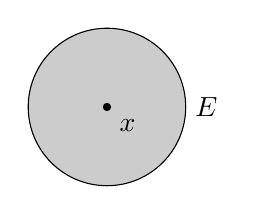
\begin{tikzpicture}
    \draw[fill=black, fill opacity=0.2] (0,0) circle (1cm);
    \node[right] at (1cm,0) {$E$};
    \node[circle, fill, minimum size=3pt, inner sep=0pt, outer sep=0pt, label=below right:$x$] at (0,0) {};
\end{tikzpicture}

$x \in E$
\end{minipage}

\bigskip
\bigskip

\begin{minipage}{\linewidth}
\centering
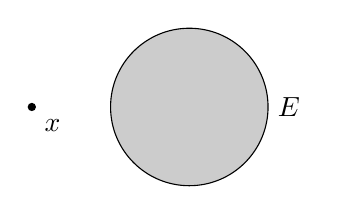
\begin{tikzpicture}
    \draw[fill=black, fill opacity=0.2] (0,0) circle (1cm);
    \node[right] at (1cm,0) {$E$};
    \node[circle, fill, minimum size=3pt, inner sep=0pt, outer sep=0pt, label=below right:$x$] at (-2cm,0) {};
\end{tikzpicture}

$x \notin E$
\end{minipage}

\bigskip
\bigskip

\begin{minipage}{\linewidth}
\centering
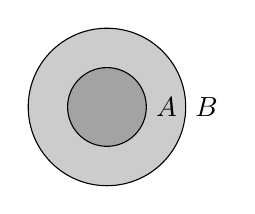
\begin{tikzpicture}
    \draw[fill=black, fill opacity=0.2] (0,0) circle (1cm);
    \draw[fill=black, fill opacity=0.2] (0,0) circle (0.5cm);
    \node[right] at (0.5cm,0) {$A$};
    \node[right] at (1cm,0) {$B$};
\end{tikzpicture}

$A \subset B$
\end{minipage}

\bigskip
\bigskip

Sur chacun des quatre schémas suivants, la zone grisée correspond à l'ensemble en légende.

\bigskip
\bigskip

\begin{minipage}{\linewidth}
\centering
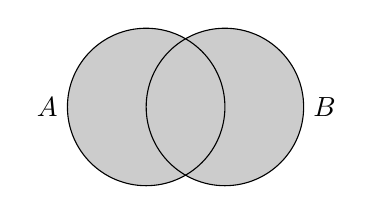
\begin{tikzpicture}
    \fill[black!20!white] (0.5cm,0) circle (1cm);
    \fill[black!20!white] (-0.5cm,0) circle (1cm);
    \draw (0.5cm,0) circle (1cm);
    \draw (-0.5cm,0) circle (1cm);
    \node[left] at (-1.5cm,0) {$A$};
    \node[right] at (1.5cm,0) {$B$};
\end{tikzpicture}

$A \cup B$
\end{minipage}

\bigskip
\bigskip

\begin{minipage}{\linewidth}
\centering
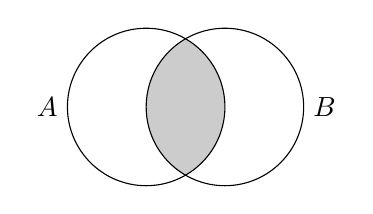
\begin{tikzpicture}
    \begin{scope}
        \clip (0.5cm,0) circle(1cm);
        \fill[black!20!white] (-0.5cm,0) circle (1cm);
    \end{scope}
    \draw (0.5cm,0) circle (1cm);
    \draw (-0.5cm,0) circle (1cm);
    \node[left] at (-1.5cm,0) {$A$};
    \node[right] at (1.5cm,0) {$B$};
\end{tikzpicture}

$A \cap B$
\end{minipage}

\bigskip
\bigskip

\begin{minipage}{\linewidth}
\centering
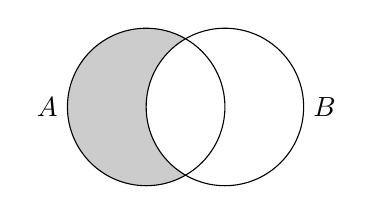
\begin{tikzpicture}
    \fill[black!20!white] (-0.5cm,0) circle (1cm);
    \begin{scope}
        \clip (0.5cm,0) circle(1cm);
        \fill[white] (-0.5cm,0) circle (1cm);
    \end{scope}
    \draw (0.5cm,0) circle (1cm);
    \draw (-0.5cm,0) circle (1cm);
    \node[left] at (-1.5cm,0) {$A$};
    \node[right] at (1.5cm,0) {$B$};
\end{tikzpicture}

$A \setminus B$
\end{minipage}

\bigskip
\bigskip

\begin{minipage}{\linewidth}
\centering
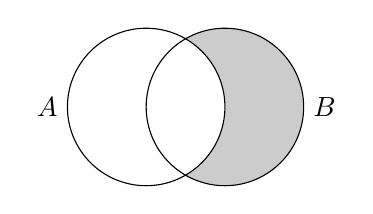
\begin{tikzpicture}
    \fill[black!20!white] (0.5cm,0) circle (1cm);
    \begin{scope}
        \clip (0.5cm,0) circle(1cm);
        \fill[white] (-0.5cm,0) circle (1cm);
    \end{scope}
    \draw (0.5cm,0) circle (1cm);
    \draw (-0.5cm,0) circle (1cm);
    \node[left] at (-1.5cm,0) {$A$};
    \node[right] at (1.5cm,0) {$B$};
\end{tikzpicture}

$B \setminus A$
\end{minipage}

\bigskip
\bigskip

Certains résultats se voient aisément schématiquement : 

\bigskip
\bigskip

\begin{minipage}{\linewidth}
\centering
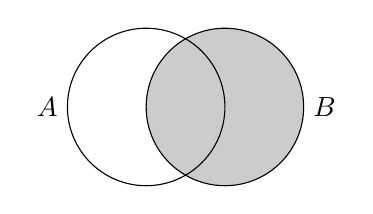
\begin{tikzpicture}
    \fill[white] (-0.5cm,0) circle (1cm);
    \fill[black!20!white] (0.5cm,0) circle (1cm);
    \draw (0.5cm,0) circle (1cm);
    \draw (-0.5cm,0) circle (1cm);
    \node[left] at (-1.5cm,0) {$A$};
    \node[right] at (1.5cm,0) {$B$};
\end{tikzpicture}

$(B \setminus A) \cup (A \cap B) = B$
\end{minipage}

\bigskip
\bigskip

\begin{minipage}{\linewidth}
\centering
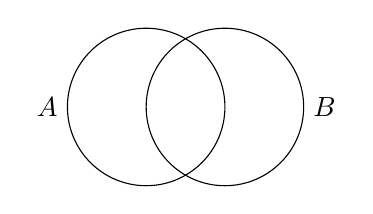
\begin{tikzpicture}
    \fill[white] (-0.5cm,0) circle (1cm);
    \fill[white] (0.5cm,0) circle (1cm);
    \draw (0.5cm,0) circle (1cm);
    \draw (-0.5cm,0) circle (1cm);
    \node[left] at (-1.5cm,0) {$A$};
    \node[right] at (1.5cm,0) {$B$};
\end{tikzpicture}

$(B \setminus A) \cap (A \cap B) = \emptyset$
\end{minipage}

\bigskip
\bigskip

\begin{minipage}{\linewidth}
\centering
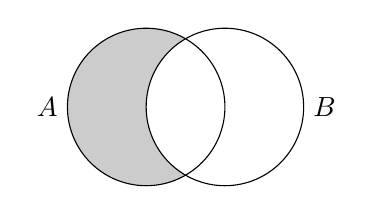
\begin{tikzpicture}
    \fill[black!20!white] (-0.5cm,0) circle (1cm);
    \fill[white] (0.5cm,0) circle (1cm);
    \draw (0.5cm,0) circle (1cm);
    \draw (-0.5cm,0) circle (1cm);
    \node[left] at (-1.5cm,0) {$A$};
    \node[right] at (1.5cm,0) {$B$};
\end{tikzpicture}

$(A \cup B) \setminus B = A \setminus B$
\end{minipage}

\bigskip
\bigskip

Une fonction d'un ensemble $E$ vers un ensemble $F$ peut être représentée par des flèches allant de chaque élément de $E$ vers son image. 

\bigskip
\bigskip

\begin{minipage}{\linewidth}
\centering
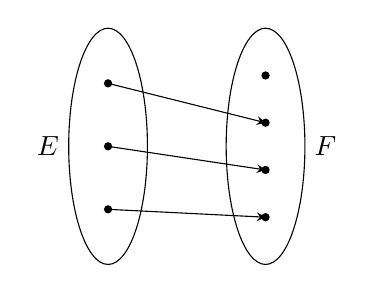
\begin{tikzpicture}
    \draw (-1cm,0) ellipse (0.5cm and 1.5cm);
    \draw (1cm,0) ellipse (0.5cm and 1.5cm);
    \node[left] at (-1.5cm,0) {$E$};
    \node[right] at (1.5cm,0) {$F$};
    \node[fill, circle, minimum size=3pt, inner sep=0, outer sep=0] at (-1cm,0.8cm) {};
    \node[fill, circle, minimum size=3pt, inner sep=0, outer sep=0] at (-1cm,0) {};
    \node[fill, circle, minimum size=3pt, inner sep=0, outer sep=0] at (-1cm,-0.8cm) {};
    \node[fill, circle, minimum size=3pt, inner sep=0, outer sep=0] at (1cm,0.9cm) {};
    \node[fill, circle, minimum size=3pt, inner sep=0, outer sep=0] at (1cm,0.3cm) {};
    \node[fill, circle, minimum size=3pt, inner sep=0, outer sep=0] at (1cm,-0.3cm) {};
    \node[fill, circle, minimum size=3pt, inner sep=0, outer sep=0] at (1cm,-0.9cm) {};
    \draw[-stealth] (-1cm,0.8cm) -- (1cm, 0.3cm);
    \draw[-stealth] (-1cm,0) -- (1cm, -0.3cm);
    \draw[-stealth] (-1cm,-0.8cm) -- (1cm, -0.9cm);
\end{tikzpicture}

Exemple d'injection
\end{minipage}

\bigskip
\bigskip

\begin{minipage}{\linewidth}
\centering
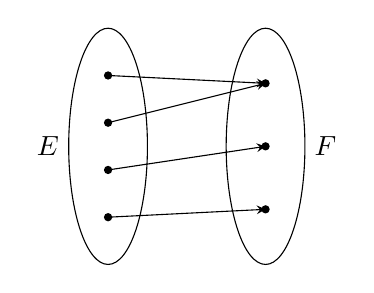
\begin{tikzpicture}
    \draw (-1cm,0) ellipse (0.5cm and 1.5cm);
    \draw (1cm,0) ellipse (0.5cm and 1.5cm);
    \node[left] at (-1.5cm,0) {$E$};
    \node[right] at (1.5cm,0) {$F$};
    \node[fill, circle, minimum size=3pt, inner sep=0, outer sep=0] at (-1cm,0.9cm) {};
    \node[fill, circle, minimum size=3pt, inner sep=0, outer sep=0] at (-1cm,0.3cm) {};
    \node[fill, circle, minimum size=3pt, inner sep=0, outer sep=0] at (-1cm,-0.3cm) {};
    \node[fill, circle, minimum size=3pt, inner sep=0, outer sep=0] at (-1cm,-0.9cm) {};
    \node[fill, circle, minimum size=3pt, inner sep=0, outer sep=0] at (1cm,0.8cm) {};
    \node[fill, circle, minimum size=3pt, inner sep=0, outer sep=0] at (1cm,0) {};
    \node[fill, circle, minimum size=3pt, inner sep=0, outer sep=0] at (1cm,-0.8cm) {};
    \draw[-stealth] (-1cm,0.9cm) -- (1cm, 0.8cm);
    \draw[-stealth] (-1cm,0.3cm) -- (1cm, 0.8cm);
    \draw[-stealth] (-1cm,-0.3cm) -- (1cm, 0);
    \draw[-stealth] (-1cm,-0.9cm) -- (1cm, -0.8cm);
\end{tikzpicture}

Exemple de surjection
\end{minipage}

\bigskip
\bigskip

\begin{minipage}{\linewidth}
\centering
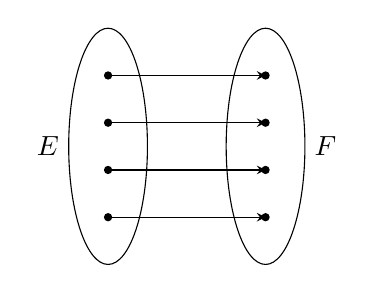
\begin{tikzpicture}
    \draw (-1cm,0) ellipse (0.5cm and 1.5cm);
    \draw (1cm,0) ellipse (0.5cm and 1.5cm);
    \node[left] at (-1.5cm,0) {$E$};
    \node[right] at (1.5cm,0) {$F$};
    \node[fill, circle, minimum size=3pt, inner sep=0, outer sep=0] at (-1cm,0.9cm) {};
    \node[fill, circle, minimum size=3pt, inner sep=0, outer sep=0] at (-1cm,0.3cm) {};
    \node[fill, circle, minimum size=3pt, inner sep=0, outer sep=0] at (-1cm,-0.3cm) {};
    \node[fill, circle, minimum size=3pt, inner sep=0, outer sep=0] at (-1cm,-0.9cm) {};
    \node[fill, circle, minimum size=3pt, inner sep=0, outer sep=0] at (1cm,0.9cm) {};
    \node[fill, circle, minimum size=3pt, inner sep=0, outer sep=0] at (1cm,0.3cm) {};
    \node[fill, circle, minimum size=3pt, inner sep=0, outer sep=0] at (1cm,-0.3cm) {};
    \node[fill, circle, minimum size=3pt, inner sep=0, outer sep=0] at (1cm,-0.9cm) {};
    \draw[-stealth] (-1cm,0.9cm) -- (1cm, 0.9cm);
    \draw[-stealth] (-1cm,0.3cm) -- (1cm, 0.3cm);
    \draw[-stealth] (-1cm,-0.3cm) -- (1cm, -0.3cm);
    \draw[-stealth] (-1cm,-0.9cm) -- (1cm, -0.9cm);
\end{tikzpicture}

Exemple de bijection
\end{minipage}

\bigskip
\bigskip

\begin{minipage}{\linewidth}
\centering
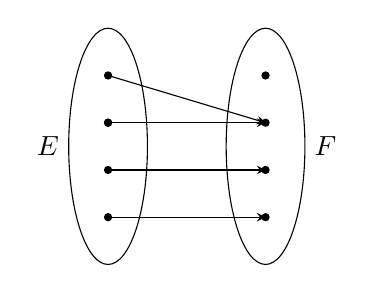
\begin{tikzpicture}
    \draw (-1cm,0) ellipse (0.5cm and 1.5cm);
    \draw (1cm,0) ellipse (0.5cm and 1.5cm);
    \node[left] at (-1.5cm,0) {$E$};
    \node[right] at (1.5cm,0) {$F$};
    \node[fill, circle, minimum size=3pt, inner sep=0, outer sep=0] at (-1cm,0.9cm) {};
    \node[fill, circle, minimum size=3pt, inner sep=0, outer sep=0] at (-1cm,0.3cm) {};
    \node[fill, circle, minimum size=3pt, inner sep=0, outer sep=0] at (-1cm,0.3cm) {};
    \node[fill, circle, minimum size=3pt, inner sep=0, outer sep=0] at (-1cm,-0.3cm) {};
    \node[fill, circle, minimum size=3pt, inner sep=0, outer sep=0] at (-1cm,-0.9cm) {};
    \node[fill, circle, minimum size=3pt, inner sep=0, outer sep=0] at (1cm,0.9cm) {};
    \node[fill, circle, minimum size=3pt, inner sep=0, outer sep=0] at (1cm,0.3cm) {};
    \node[fill, circle, minimum size=3pt, inner sep=0, outer sep=0] at (1cm,-0.3cm) {};
    \node[fill, circle, minimum size=3pt, inner sep=0, outer sep=0] at (1cm,-0.9cm) {};
    \draw[-stealth] (-1cm,0.9cm) -- (1cm, 0.3cm);
    \draw[-stealth] (-1cm,0.3cm) -- (1cm, 0.3cm);
    \draw[-stealth] (-1cm,-0.3cm) -- (1cm, -0.3cm);
    \draw[-stealth] (-1cm,-0.9cm) -- (1cm, -0.9cm);
\end{tikzpicture}

Exemple de fonction ni injective ni bijective
\end{minipage}


\subsection{Construction de \texorpdfstring{$\mathbb{N}$}{N}}
\label{sub:constN}

\subsubsection{Définition}

L'ensemble des entiers naturels, noté $\mathbb{N}$, est défini de la manière suivante. 
Notons $\mathrm{Cl}$ le prédicat à un paramètre libre défini par :
\begin{equation*}
    \mathrm{Cl}(A): (\emptyset \in A) \wedge (\forall a \, (a \in A \Rightarrow a \cup \lbrace a \rbrace \in A)). 
\end{equation*}
D'après l'axiome de l'infini, il existe un ensemble $A$ tel que $\mathrm{Cl}(A)$ est vrai.
Soit $\mathrm{Ent}$ le prédicat à un paramètre libre défini par : 
\begin{equation*}
    \mathrm{Ent}(x): \forall A \, (\mathrm{Cl}(A) \Rightarrow x \in A). 
\end{equation*}
Soit $I$ un ensemble tel que $\mathrm{Cl}(I)$ est vrai. 
L'ensemble $\mathbb{N}$ est défini par : 
\begin{equation*}
     \mathbb{N} = \lbrace x \in I \vert \mathrm{Ent}(x) \rbrace. 
\end{equation*}
Notons que cette définition ne dépend pas du choix de $I$. 
Notons aussi que $\emptyset \in \mathbb{N}$ et $\forall n \, n \in \mathbb{N} \Rightarrow n \cup \lbrace n \rbrace \in \mathbb{N}$.

\medskip

\noindent\textbf{Démonstration :}

\begin{itemize}[nosep]
    \item Montrons d'abord que $\emptyset \in \mathbb{N}$. 
        Puisque $\mathrm{Cl}(I)$ est vrai, $\emptyset \in I$.
        Soit $A$ un ensemble tel que $\mathrm{Cl}(A)$ est vrai.
        Alors, $\emptyset \in A$.
        Donc, $\mathrm{Ent}(\emptyset)$ est vrai. 
        On a donc $\emptyset \in I \wedge \mathrm{Ent}(\emptyset)$. 
        Donc, $\emptyset \in \mathbb{N}$.
    \item Soit $n$ un élément de $\mathbb{N}$. 
        Alors, $n \in I$.
        Puisque $\mathrm{Cl}(I)$ est vrai, on en déduit que $n \cup \lbrace n \rbrace \in I$.
        Soit $A$ un ensemble tel que $\mathrm{Cl}(A)$ est vrai.
        Puisque $\mathrm{Ent}(n)$ est vrai, $n \in A$.
        Alors, puisque $\mathrm{Cl}(A)$ est vrai, $n  \cup \lbrace n \rbrace \in A$.
        On en déduit que $\mathrm{Ent}(n  \cup \lbrace n \rbrace)$ et vrai. 
        On a donc $n  \cup \lbrace n \rbrace \in I \wedge \mathrm{Ent}(n  \cup \lbrace n \rbrace)$. 
        Donc, $n  \cup \lbrace n \rbrace \in \mathbb{N}$.
    \item Motrons finalement que la définition de $\mathbb{N}$ ne dépends pas du choix de $I$. 
        Soit $J$ un ensemble tel que $\mathrm{Cl}(J)$ est vrai.
        Soit $\mathbb{M}$ l'ensemble défini par : $\mathbb{M} = \lbrace x \in J \vert \mathrm{Ent}(x) \rbrace$. 
        Il s'agit de montrer que $\mathbb{M} = \mathbb{N}$. \\
        Soit $x$ un élément de $\mathbb{N}$. 
        Puisque $\mathrm{Cl(J)}$ et $\mathrm{Ent(x)}$ sont vrais, $x \in J$ est vrai aussi. 
        Donc, $x \in J \wedge \mathrm{Ent}(x)$. 
        Donc, $x \in \mathbb{M}$. 
        Cela montre que $\mathbb{N} \subset \mathbb{M}$. \\
        Soit $y$ un élément de $\mathbb{M}$. 
        Puisque $\mathrm{Cl(I)}$ et $\mathrm{Ent(y)}$ sont vrais, $y \in I$ est vrai aussi. 
        Donc, $y \in I \wedge \mathrm{Ent}(x)$. 
        Donc, $y \in \mathbb{N}$. 
        Cela montre que $\mathbb{M} \subset \mathbb{N}$. \\
        On a donc $\mathbb{M} = \mathbb{N}$.
\end{itemize}

\done

\medskip

On notera souvent $0$ l'ensemble $\emptyset$. 
Pour tout élément $n$ de $\mathbb{N}$, on notera $n+1$ l'ensemble $n \cup \lbrace n \rbrace$, appelé \textit{successeur} de $n$. 
Cela définit une application $\mathrm{Suc}$ de $\mathbb{N}$ vers lui-même, qui à un élément $n$ associe $n+1$. 
Notons que, pour tout entier naturel $n$, on a $n \subset n+1$.
Les premiers entiers sont notés de la manière suivante en base $10$ (voir section~\ref{sub:base} pour une définition générale de la base) : 

\begin{center}
\begin{tabular}{c | c}
    n & n+1 \\
    \hline 
    0 & 1 \\
    1 & 2 \\
    2 & 3 \\
    3 & 4 \\
    4 & 5 \\
    5 & 6 \\
    6 & 7 \\
    7 & 8 \\
    8 & 9 \\
    9 & 10 \\
\end{tabular}
\end{center}

\noindent\textbf{NB:} Notons que $\mathrm{Cl}(\mathbb{N})$ est vraie et, si $E$ est un ensemble tel que $\mathrm{Cl}(E)$ est vraie, alors $\mathbb{N} \subset E$. 
En ce sens, $\mathbb{N}$ est le plus petit ensemble satisfaisant $\mathrm{Cl}$.

\medskip

\noindent\textbf{Démonstration :}

Tout d'abord, on a vu ci-dessus que $\emptyset \in \mathbb{N}$ et $\forall n \, n \in \mathbb{N} \Rightarrow n \cup \lbrace n \rbrace \in \mathbb{N}$. 
Donc, $\mathrm{Cl}(\mathbb{N})$ est vrai. 

Soit $E$ un ensemble tel que $\mathrm{Cl}(E)$ est vrai. 
Soit $x$ un élément de $\mathbb{N}$. 
Alors, $\mathrm{Ent}(x)$ est vrai, donc $x \in E$. 
Ainsi, $\mathrm{N} \subset E$. 

\done

\medskip

Un élément de $\mathbb{N}$ est dit \textit{entier naturel} (ou parfois simplement \textit{entier} quand il n'y a pas de confusion possible avec d'autres définitions). 
Il est dit \textit{non nul} s'il est différent de $0$.

\medskip

\noindent\textbf{Lemme :} Soit $n$ un élément de $\mathbb{N}$ et $m$ un ensemble tel que $m \subset n+1$. 
    Alors $n \in m$ ou $m \subset n$.

\medskip

\noindent\textbf{Démonstration :}
    Si $n \in m$, le résultat est vrai. 
    Supposons que $n \notin m$. 
    Soit $x$ un élément de $m$. 
    Puisque $m \subset n+1$, on a $x \in n+1$, et donc $x \in n$ ou $x \in \lbrace n \rbrace$. 
    La seconde option est impossible puisqu'elle impliquerait $x = n$, et donc $n \in m$, en contradiction avec notre hypothèse. 
    Donc, $x \in n$. 
    Cela étant vrai pour tout élément $x$ de $m$, on en déduit $m \subset n$.

   \done 

\medskip

\noindent\textbf{Définition :} 
    On note $\mathbb{N}^*$ l'ensemble $\mathbb{N} \setminus \lbrace 0 \rbrace$.

\subsubsection{Relation d'ordre : définition}

On définit une relation binaire, notée $\leq$, sur $\mathbb{N}$ par : pour tous éléments $n$ et $m$ de $\mathbb{N}$, 
\begin{equation*}
    n \leq m \Leftrightarrow n \subset m .
\end{equation*}
Il sagit d'une relation d'ordre puisque la relation $\subset$ est réflexive, antisymétrique et transitive.
On définit la relation d'ordre strict $<$ par pour tous éléments $n$ et $m$ de $\mathbb{N}$, 
\begin{equation*}
    n < m \Leftrightarrow (n \leq m \wedge m \neq n).
\end{equation*}
Notons que, pour tout élément $n$ de $\mathbb{N}$, $0 \leq n$ (puisque l'ensemble vide est un sous-ensemble de tout ensemble) et $n < n+1$ (en effet, on a $n \subset n+1$, donc $n \leq n+1$, et $n \neq n+1$ ; nous démontrerons ce point dans la Section~\ref{subsub:relOrdreProps}—pour le moment, nous avons seulement montré que $n \leq n+1$). 
Par antisymétrie, le premier point implique que le seul élément $n$ de $\mathbb{N}$ satisfaisant $n \leq 0$ est $0$ lui-même.

On définit aussi la relation d'ordre $\geq$ et la relation d'ordre strict $>$ sur $\mathbb{N}$ par : pour tous éléments $n$ et $m$ de $\mathbb{N}$, $n \geq m \Leftrightarrow m \leq n$ et $n > m \Leftrightarrow m < n$.

\subsubsection{Principe de récurrence}
\label{subsub:recurrence}

\noindent\textbf{Lemme (principe de récurrence) :} Soit $P$ une formule à un paramètre libre. 
    On suppose que $P(0)$ est vraie et que, pour tout élément $n$ de $\mathbb{N}$, $P(n) \Rightarrow P(n+1)$ est vraie. 
    Alors, $P(n)$ est vraie pour tout $n \in \mathbb{N}$.

\medskip

\noindent\textbf{Démonstration :} Soit $E$ l'ensemble défini par $E = \lbrace n \in \mathbb{N} \vert P(n) \rbrace$. 
    Puisque $P(0)$ et vraie, on a $0 \in E$. 
    En outre, pour tout $n \in E$, $P(n)$ est vrai, donc $P(n+1)$ est vrai aussi, et donc $n+1 \in E$. 
    Donc, $\mathrm{Cl}(E)$ est vraie. 
    Donc, $\mathbb{N} \subset E$. 
    Soit $n \in \mathbb{N}$, on a donc $n \in E$, et donc $P(n)$ est vraie.

   \done 

\medskip

\noindent\textbf{Récurrence finie :} Soit $E$ un sous-ensemble non vide de $\mathbb{N}$ tel que : $\forall n \in E, \, \forall m \in \mathbb{N}, \, m \leq n \Rightarrow m \in E$. 
    Soit $P$ une formule à un paramètre libre. 
    On suppose que $P(0)$ est vraie et que, pour tout $n \in E$ tel que $n+1 \in E$, $P(n) \Rightarrow P(n+1)$ est vraie. 
    Alors, $P(n)$ est vraie pour tout $n \in E$.

\medskip

\noindent\textbf{Démonstration :} Notons que $0 \in E$. Définissons la formule $Q$ à un paramètre libre par $Q(n): P(n) \vee (n \notin E)$.
    Alors $Q(0)$ est vraie. 
    En outre, soit $n \in \mathbb{N}$ tel que $Q(n)$ est vraie, soit $n+1 \in E$, donc $n \in E$, donc $P(n)$ est vraie, donc $P(n+1)$ est vraie, et donc $Q(n+1)$ est vraie, soit $n+1 \notin E$ et donc $Q(n+1)$ est vraie.
    Par récurrence, $Q(n)$ est vraie pour tout $n \in \mathbb{N}$.
    Soit $n \in E$. 
    Puisque $Q(n)$ est vraie et que $n \notin E$ ne peut être vraie, on en déduit que $P(n)$ est vraie.

   \done 

\medskip

Donnons un exemple facile de démonstration par récurrence. 

\medskip

\noindent\textbf{Lemme :} Soit $n$ un entier naturel. Alors $n=0$ ou il existe un entier naturel $m$ tel que $n=m+1$.

\medskip

\noindent\textbf{Remarque :} On montre Section~\ref{subsub:relOrdreProps} que deux entiers naturels $a$ et $b$ satisfaisant $a+1=b+1$ sont égaux. Donc, l'entier naturel $m$ défini par l'énoncé du lemme est unique. 

\medskip

\noindent\textbf{Démonstration :} Soit $P$ le prédicat à un paramètre défini par : $P(n): n=0 \vee (\exists m \in \mathbb{N}, \, n=m+1)$. 
    Tout d'abord, $P(0)$ est vrai puisque $0=0$ est vrai.
    Soit $n$ un élément de $\mathbb{N}$. 
    Alors $P(n+1)$ est vrai puisqu'il existe un entier naturel $m$ tel que $n+1 = m+1$—il suffit de prendre $m=n$. 
    Par récurrence, $P(n)$ est donc vrai pour tout élément $n$ de $\mathbb{N}$.

   \done 

\medskip

\noindent\textbf{Définition :} Soit $n$ un entier naturel tel que $n \neq 0$. L'entier naturel $m$ tel que $n=m+1$ est noté $n-1$.
    Notons que, pour tout entier naturel $n$, $(n+1)-1 = n$ et, si $n \neq 0$, $(n-1)+1 = n$.

\medskip 

Cet exemple est conceptuellement très simple car la seconde étape du raisonnement ne fait pas appel au fait que le prédicat est vrai au rang précédent. 
Donnons maintenant un exemple légèrement moins aisé, et plus proche de la manière dont la démonstration par récurrence fonctionne la plupart du temps. 
On admet momentanément que, pour tout entier naturel $n$, $n+1 \neq n$, et donc $n \notin n$. 
(Cela sera démontré, sans utiliser le lemme suivant, section~\ref{subsub:relOrdreProps}.)

\medskip

\noindent\textbf{Lemme :} Soit $n$ et $m$ deux entiers naturels. S'il existe une bijection de $n$ vers $m$, alors $n=m$.

\medskip

\noindent\textbf{Démonstration :} Considérons le prédicat suivant, dépendant d'un paramètre libre $n$ : \textit{Pour tout entier naturel $m$, s'il existe une bijection de $n$ vers $m$, alors $n=m$.} 

    Pour $n=0$, le résultat est aisé : la seule fonction de $0$ vers un ensemble est $\emptyset$, dont l'image est $\emptyset$. 
    Si $E$ est un ensemble et s'il existe une biection de $0$ vers $E$, alors $E = \emptyset = 0$.

    Soit $n$ un entier naturel pour lequel le prédicat est vrai. 
    Soit $m$ un entier naturel et $f$ une bijection de $n+1$ vers $m$. 
    Puisqu'une telle bijection existe et $n+1$ est non vide (il contient au moins $n$), $m$ ne peut être égal à $0$ (il contient au moins les images des éléments de $n+1$). 
    Donc, d'après le lemme précédent, on peut choisir un entier naturel $k$ tel que $m = k+1$. 
    Montrons qu'il existe une bijection de $n$ vers $k$. 
    On aura alors $n=k$, donc $n+1=k+1$, et donc $n+1=m$, et le lemme sera montré par récurrence.

    On a : $m = k \cup \lbrace k \rbrace$. 
    Soit $g$ la fonction de $m$ vers $m$ définie par $g(k) = f(n)$, $g(f(n)) = k$ (notons que cela est toujours possible car ces deux conditions sont équivalentes si $f(n)=k$) et $g(x)=x$ pour tout élément $x$ de $m$ tel que $x \notin \lbrace k, f(n) \rbrace$. 
    Supposons avoir montré que $g$ est une bijection de $m$ vers $m$. 
    Alors, $g \circ f$ est une bijection de $n+1$ vers $m$ et $(g \circ f)(n) = k$. 
    Soit $h$ la fonction de $n$ vers $k$ définie par : pour tout élément $x$ de $n$, $h(x) = (g \circ f)(x)$. 
    (Son image est bien incluse dans $k$ puisque, pour tout élément $x$ de $n$, $(g \circ f)(x) \in m$ et $(g \circ f)(x) \neq k$ puisque $x \neq n$ (car $x \in n$ et $n \notin n$).)
    Montrons que $h$ est une bijection. 
    Soit $x$ et $y$ deux éléments de $n$ tels que $h(x)=h(y)$.
    Alors, $(g \circ f)(x) = (g \circ f)(y)$.
    Puisque  $g \circ f$ est une bijection, cela implique $x=y$.
    Donc, $h$ est injective. 
    Soit $y$ un élément de $k$. 
    Puisque $g \circ f$ est bijective, on peut choisir un élément $x$ de $n+1$ tel que $(g \circ f)(x) = y$. 
    En outre, $y \in k$, donc $y \neq k$. 
    Puisque $(g \circ f)(n)=k$, cela implique $x \neq n$, et donc $x \in n$. 
    On a donc $h(x) = y$. 
    Donc, $h$ est surjective.
    La fonction $h$ est ainsi une bijection de $n$ vers $k$.

    Il nous reste à montrer que la fonction $g$ est bijective. 
    Montrons d'abord qu'elle est injective. 
    Soit $x$ et $y$ deux éléments de $m$ tels que $g(x) = g(y)$.
    Si ni $x$ ni $y$ ne sont dans $\lbrace f(n), k \rbrace$, alors $g(x) = x$ et $g(y) = y$, donc $x=y$. 
    Si $x \in \lbrace f(n), k \rbrace$, alors $y \in \lbrace f(n), k \rbrace$ (sans quoi on aurait $g(x) \in \lbrace f(n), k \rbrace$ et $g(y) \notin \lbrace f(n), k \rbrace$). 
    De même, si $y \in \lbrace f(n), k \rbrace$, alors $x \in \lbrace f(n), k \rbrace$. 
    Supposons $x = k$. 
    Alors, $g(x) = f(n)$, donc $g(y) = f(n)$. 
    Si $y = f(n)$, on a $g(y) = k$, ce qui contredit $g(x) = g(y)$ sauf si $f(n) = k$. 
    Donc, $y = k$ ou $y = f(n)$ et $f(n) = k$. 
    Dans les deux cas, on a $y = k$, et donc $y = x$. 
    Enfin, supposons $x = f(n)$. 
    Alors, $g(x) = k$, donc $g(y) = k$. 
    Si $y = k$, on a $g(y) = f(n)$, ce qui contredit $g(x) = g(y)$ sauf si $k = f(n)$. 
    Donc, $y = f(n)$ ou $y = k$ et $k = f(n)$. 
    Dans les deux cas, on a $y = f(n)$, et donc $y = x$. 
    Ainsi, $g$ est bien injective. 

    Montrons qu'elle est surjective. 
    Soit $y$ un élément de $m$. 
    Si $y \notin \lbrace k, f(n) \rbrace$, on a $g(y) = y$. 
    Si $y \in \lbrace k, f(n) \rbrace$, on a $y = k$ ou $y = f(n)$. 
    Dans le premier cas, $g(f(n)) = y$. 
    Dans le second cas, $g(k) = y$. 
    Dans tous les cas, il existe donc un élément $x$ de $m$ tel que $g(x) = y$. 
    Ainsi, $g$ est surjective. 
    Il s'agit donc bien d'une bijection. 

   \done 

\subsubsection{Relation d'ordre : propriétés}
\label{subsub:relOrdreProps}

\noindent\textbf{Lemme :} Pour tout élément $n$ de $\mathbb{N}$, $0 \leq n$.

\medskip

\noindent\textbf{Démonstration :} Évident car $\emptyset \subset E$ pour tout ensemble $E$. 

   \done 

\noindent\textbf{Lemme :} Pour tout élément $n$ de $\mathbb{N}$, $n \leq 0 \Rightarrow n = 0$.

\medskip

\noindent\textbf{Corrolaire :} Il n'existe aucun élément $n$ de $\mathbb{N}$ tel que $n < 0$.

\medskip

\noindent\textbf{Démonstration :} Conséquence directe du lemme précédent et de l'antisymétrie de $\leq$. 

   \done 

\medskip

\noindent\textbf{Lemme :} Pour tout élément $n$ de $\mathbb{N}$, on a $n \neq 0 \Rightarrow 0 \in n$.

\medskip

\noindent\textbf{Démonstration :} 
    On procède par récurrence. 
    Soit $P: n \neq 0 \Rightarrow 0 \in n$.
    Pour $n = 0$, le résultat est évident car $n \neq 0$ est fausse, donc $P(0)$ est vraie. 
    Soit $n$ un élément de $\mathbb{N}$ tel que $P(n)$ est vraie. 
    Si $n = 0$, $n+1 = \lbrace \emptyset \rbrace$, donc $0 \in n+1$, donc $P(n+1)$ est vraie.
    Si $n \neq 0$, $0 \in n$, donc, puisque $n \subset n+1$, $0 \in n+1$, donc $P(n+1)$ est vraie.
    Par récurrence, on en déduit que $P(n)$ est vraie pour tout élément $n$ de $\mathbb{N}$.

   \done 

\medskip

\noindent\textbf{Lemme :} 
    Soit $n$ un élément de $\mathbb{N}$. 
    Pour tout élément $m$ de $\mathbb{N}$ tel que $n \leq m$, on a $m \notin n$.
    En particulier, pour tout élément $n$ de $\mathbb{N}$, on a $n+1 \neq n$. 
    Puisque $n \subset n+1$, $n \leq n+1$, donc cela implique $n < n+1$. 

\medskip

\noindent\textbf{Démonstration :} 
    Montrons d'abord que la première partie du lemme implique bien le cas particulier. 
    Soit $n$ un élément de $\mathbb{N}$. 
    On a $n \in n+1$. 
    Si la première partie du lemme est vraie, on a aussi $n \notin n$, d'où $n+1 \neq n$.

    Montrons maintenant la première partie du lemme. 
    On procède par récurrence. 
    La propriété attendue est évidente pour $0$ puisqu'il s'agit de l'ensemble vide. 

    Soit $n$ un élément de $\mathbb{N}$ et supposons que, pour tout élément $m$ de $\mathbb{N}$ tel que $n \leq m$, $m \notin n$. 
    Soit $m$ un élément de $\mathbb{N}$ tel que $n+1 \leq m$. 
    Puisque $n \subset n+1$ et $n+1 \subset m$, on a $n \subset m$, et donc $n \leq m$.
    Donc, $m \notin n$. 
    En outre, $n \in n+1$ et $n \notin n$ (puisque $n \leq n$), donc $n+1 \subset n$ ne peut être vrai, donc $m \neq n$, donc $m \notin \lbrace n \rbrace$. 
    Puisque $n+1 = n \cup \lbrace n \rbrace$, on en déduit $m \notin n+1$. 
    La propriété attendue est donc vraie pour $n+1$.

    Par récurrence, la propriété est vraie pour tout élément $n$ de $\mathbb{N}$.

   \done 

\medskip

\noindent\textbf{Lemme :} 
    Soit $n$ un élément de $\mathbb{N}$. 
    Pour tout élément $m$ de $\mathbb{N}$ tel que $m \in n$, on a $n > m$.

\medskip

\noindent\textbf{Démonstration :} 
    On procède par récurrence sur $n$. 
    Pour $n = 0$, le résultat est évident puisqu'aucun élément $m$ de $\mathbb{N}$ ne satisfait $m \in 0$.
    Soit $n$ un élément de $\mathbb{N}$ satisfaisant la propriété énoncée dans le lemme. 
    Soit $m$ un élément de $\mathbb{N}$ tel que $m \in n+1$. 
    Alors, $m \in n$ ou $m = n$.
    \begin{itemize}[nosep]
        \item Si $m \in n$, on a $n > m$.
            En outre, d'après le lemme précédent, on a $n+1 > n$. 
            Donc, $n+1 > m$.
        \item Si $m = n$, on a $n+1 > m$ d'après le lemme précédent.
    \end{itemize}
    Ainsi, $n+1$ satisfait également la propriété énoncée dans le lemme. 
    Par récurrence, on en déduit qu'elle est vraie pour tout élément $n$ de $\mathbb{N}$.
    
   \done 

\medskip

\noindent\textbf{Lemme :} 
    Soit $n$ un élément de $\mathbb{N}$. 
    Pour tout élément $m$ de $\mathbb{N}$ tel que $m < n$, on a $m \in n$.

\medskip

\noindent\textbf{Démonstration :} 
    On procède par récurrence. 
    Pour $n=0$, le résultat est évident puisqu'il n'existe aucun élément $m$ de $\mathbb{N}$ tel que $m < 0$.
    Soit $n$ un élément de $\mathbb{N}$ tel que, pour tout élément $m$ de $\mathbb{N}$ tel que $m < n$, $m \in n$. 
    Soit $m$ un élément de $\mathbb{N}$ tel que $m < n+1$. 
    Montrons d'abord que $n \notin m$. 
    Si on avait $n \in m$, alors on aurait $m > n$ d'après le lemme précédent, d'où $n \subset m$ et (puisque $n \in m$) $n+1 \subset m$, en contradiction avec $m < n+1$. 
    Donc, $n \notin m$. 
    Donc, puisque $m \subset n+1$, $m \subset n$. 
    (En effet, soit $x$ un élément de $m$, on a $x \in n+1$, donc $x \in n$ ou $x \in \lbrace n \rbrace$ ; la seconde option est impossible car $n \notin m$, donc $m \in n$.)
    Donc, $m \leq n$. 
    Si $m = n$, on a $m \in n+1$. 
    Sinon, $m < n$, donc $m \in n$, et donc $m \in n+1$. 
    Dans les deux cas, $m \in n+1$. 
    Ainsi, la propriété énoncée dans le lemme est vraie pour $n+1$. 
    Par récurrence, on en déduit qu'elle l'est pour tout élément $n$ de $\mathbb{N}$.

   \done 

\medskip

\noindent\textbf{Corrolaire :} 
    Soit $n$ et $m$ deux éléments de $\mathbb{N}$. 
    D'après les deux lemmes précédents, les propositions $m \in n$ et $m < n$ sont équivalentes.

\medskip

\noindent\textbf{Lemme :} 
    Soit $n$ un élément de $\mathbb{N}$. 
    Pour tout élément $m$ de $\mathbb{N}$ tel que $m \notin n$, on a $n \leq m$.

\medskip

\noindent\textbf{Démonstration :} 
    On procède par récurrence sur $n$. 
    Pour $n=0$, le résultat est évident car $0 \leq m$ pour tout élément $m$ de $\mathbb{N}$.
    Soit $n$ un élément de $\mathbb{N}$ tel que, pour tout élément $m$ de $\mathbb{N}$ tel que $m \notin n$, $n \leq m$. 
    Soit $m$ un élément de $\mathbb{N}$ tel que $m \notin n+1$. 
    Alors, $m \notin n$ (donc $n \leq m$) et $m \neq n$, donc $n < m$. 
    D'après le lemme précédent, cela implique $n \in m$. 
    Puisque $n < m$, on a en outre $n \subset m$. 
    Donc, $n+1 \subset m$. 
    Donc, $n+1 \leq m$. 
    On en déduit que le résultat est vrai pour $n+1$.
    Par récurrence, il est vrai pour tout élément $n$ de $\mathbb{N}$. 

   \done 

\medskip

\noindent\textbf{Corrolaire :} 
    Soit $n$ et $m$ deux élément de $\mathbb{N}$. 
    Les formules $m \notin n$ et $n \leq m$ sont équivalentes.

\medskip

\noindent\textbf{Démonstration :} 
    Soit $n$ et $m$ deux éléments de $\mathbb{N}$. 
    Si $n \leq m$, alors $n \subset m$. 
    Puisque $m \notin m$, cela implique $m \notin n$. 
    Donc, $(n \leq m) \Rightarrow (m \notin n)$.
    Le lemme précédent montre en outre que $(n \leq m) \Leftarrow (m \notin n)$.
    Donc, $(n \leq m) \Leftrightarrow (m \notin n)$.
    
   \done 

\medskip

\noindent\textbf{Corrolaire :} Soit $n$ et $m$ deux éléments de $\mathbb{N}$ tels que $n \notin m$ et $m \notin n$. 
    Alors $m \leq n$ et $n \leq m$, et donc $n = m$.

\medskip

\noindent\textbf{Lemme :} La relation d'ordre $\leq$ sur $\mathbb{N}$ est une relation d'ordre total.

\medskip

\noindent\textbf{Démonstration :} 
    Soit $n$ et $m$ deux éléments de $\mathbb{N}$. 
    Alors, $m \in n$ ou $m \notin n$. 
    Dans le premier cas, $n > m$, donc $m < n$, et donc $m \leq n$.
    Dans le second cas, $n \leq m$.

   \done 

\medskip

\noindent\textbf{Corrolaire :} Soit $n$ et $m$ deux éléments de $\mathbb{N}$. 
    Si $n \leq m$ est fausse, alors $m \leq n$ est vraie (d'après le lemme précédent) et $n \neq m$ est vraie (car $n \leq n$), donc $m < n$ est vraie. 
    Donc, $\neg (n \leq m) \Rightarrow (m < n)$. 
    Par ailleurs, si $m < n$, alors $n \leq m$ est fausse (sans quoi on aurait $m \subset n$ et $n \subset m$, et donc $m = n$).
    Ainsi, $\neg (n \leq m)$ est équivalente à $m < n$, et donc à $n > m$.
    De même, $\neg (n \geq m)$ est équivalente à $m > n$, et donc à $n < m$.

\medskip

\noindent\textbf{Corrolaire :} Soit $n$ et $m$ deux éléments de $\mathbb{N}$. 
    Puisque $\leq$ est une relation d'ordre totale, on a $n \leq m$ ou $n \geq m$. 
    Donc, $n < m$ ou $n = m$ ou $n > m$. 

\medskip

Notons que, si deux éléments $n$ et $m$ de $\mathbb{N}$ satisfont $n+1 = m+1$, on a soit $n = m$ soit $n \in m$ et $m \in n$.%
\footnote{
    En effet, puisque $n \in n+1$ et $m \in m+1$, la formule $n+1 = m+1$ implique $(n \in m+1) \wedge (m \in n+1)$, d'où $((n = m) \vee (n \in m)) \wedge ((m = n) \vee (m \in n))$. 
    En utilisant deux fois la distributivité de $\wedge$ sur $\vee$ ainsi que sa symétrie, cette formule se récris $((n = m) \wedge (m = n)) \vee ((n = m) \wedge (m \in n)) \vee ((n \in m) \wedge (m = n)) \vee ((n \in m) \wedge (m \in n))$. 
    Puisque $(n = m) \wedge (m \in n)$ et $(n \in m) \wedge (m = n)$ ne peuvet être vraies, et par symétrie de l'égalité, cette formule est équivalente à $(n = m) \vee (n \in m) \wedge (m \in n)$.
}
La seconde possibilité implique $m < n$ et $n < m$, qui ne peuvent être stisfaites simultanément (car cela impliquerait $m \leq n$ et $n \leq m$, d'où $n = m$, ce qui est incompatible avec $m < n$). 
On en déduit le lemme suivant :

\medskip

\noindent\textbf{Lemme :} 
    Soit $n$ et $m$ deux éléments de $\mathbb{N}$. 
    Si $n+1 = m+1$, alors $n=m$.

\medskip

\noindent\textbf{Lemme :} 
    Soit $n$ un élément de $\mathbb{N}$. 
    Pour tout élément $m$ de $\mathbb{N}$ tel que $m < n+1$, on a $m \leq n$. 
    La réciproque est évidente puisque $n < n+1$ : pour tout élément $m$ de $\mathbb{N}$, si $m \leq n$, $m < n+1$. 
    Donc, pour tout élément $m$ de $\mathbb{N}$, on a $m < n+1 \Leftrightarrow m \leq n$. 

\medskip

\noindent\textbf{Corrolaire :} 
    En prenant la négation de la formule de chaque côté du connecteur $\Leftrightarrow$, on obtient, pour tout élément $m$ de $\mathbb{N}$ : $m \geq n+1 \Leftrightarrow m > n$.

\medskip

\noindent\textbf{Démonstration :} 
    Soit $m$ un élément de $\mathbb{N}$ tel que $m < n+1$. 
    Alors $m \subset n \cup \lbrace n \rbrace$. 
    Si $n \in m$, on a $m > n$, donc $n \subset m$, et donc $n+1 \subset m$ et donc $n+1 \leq m$, ce qui est impossible par hypothèse. 
    On en déduit que $n \notin m$, donc que $m \subset n$, et donc que $m \leq n$. 
    Ainsi, $\forall m \in \mathbb{N}\, m < n+1 \Rightarrow m \leq n$. 
    Cela montre la première partie du lemme, de laquelle le reste découle. 
    
   \done 

\medskip

\noindent\textbf{Lemme :} 
    Pour tout entier naturel $n$, on a : $n = \lbrace m \in \mathbb{N} \vert m < n \rbrace$. 

\medskip

\noindent\textbf{Démonstration :} 
    On procède par récurrence. 
    Tout d'abord, il n'existe aucun entier naturel $m$ tel que $m < 0$. 
    Donc, $\lbrace m \in \mathbb{N} \vert m < 0 \rbrace = \emptyset = 0$. 
    Soit $n$ un entier naturel tel que $n = \lbrace m \in \mathbb{N} \vert m < n \rbrace$. 
    Puisque $n+1 = n \cup \lbrace n \rbrace$, on a : $n + 1 = \lbrace m \in \mathbb{N} \vert m < n \vee m = n \rbrace$. 
    Cela peut se récrire : $n + 1 = \lbrace m \in \mathbb{N} \vert m \leq n \rbrace$. 
    D'après le lemme précédent, cela est équivalent à : $n + 1 = \lbrace m \in \mathbb{N} \vert m < n + 1 \rbrace$. 
    Par récurrence, le résultat attendu est donc vrai pour tout entier naturel.
    
   \done 

\medskip

\noindent\textbf{Lemme (récurrence en partant d'un rang non nul) :} 
    Soit $n$ un entier naturel et $P$ un prédicat à un paramètre. 
    On suppose que $P(n)$ est vrai et que, pour tout entier naturel $m$ tel que $m \geq n$, $P(m) \Rightarrow P(m+1)$. 
    Alors, $\forall m \in \mathbb{N}, \, m \geq n \Rightarrow P(n)$.

\medskip

\noindent\textbf{Démonstration :} On procède par récurrence. 
    Soit $Q$ le prédicat à un paramètre libre défini par $Q(m): m \geq n \Rightarrow P(n)$.
    Si $n = 0$, $P(0)$ est vrai, donc $Q(0)$ l'est aussi. 
    Si $n \neq 0$, $n > 0$, donc $0 \geq n$ est fausse et $Q(0)$ est vraie. 
    Dans  tous les cas, $Q(0)$ est vraie. 

    Soit $m$ un entier naturel tel que $Q(m)$ est vrai. 
    Alors, 
    \begin{itemize}[nosep]
        \item Si $m+1 < n$, $n \geq m+1$ est fausse, donc $Q(m+1)$ est vrai.
        \item Si $m+1 = n$, $P(m+1)$ est vrai, donc $Q(m+1)$ est vrai.
        \item Si $m+1 > n$, $m \geq n$, donc $P(m)$ est vrai (puisque $Q(m)$ l'est), donc $P(m+1)$ est vrai, donc $Q(m+1)$ est vrai.
    \end{itemize}
    On a donc montré que, pour tout entier naturel $m$, $Q(m) \Rightarrow Q(m+1)$. 
    Par récurrence, $Q(m)$ est donc vrai pour tout entier naturel $m$.

   \done 

\medskip

\noindent\textbf{Définition :} Soit $a$ et $b$ deux entiers naturels. 
    On définit l'ensemble $[\![a, b]\!]$ par : 
    \begin{equation*}
        [\![a, b]\!] = \lbrace n \in \mathbb{N} \vert (n \geq a) \wedge (n \leq b) \rbrace.
    \end{equation*}
    Notons que $[\![a, b]\!] = \emptyset$ si $a > b$. 
    En effet, dans ce cas, tout élément $x$ de $\mathbb{N}$ satisfaisant $x \geq a$ satisfait $x > b$, et donc ne satistfait pas $x \geq b$.

\medskip

\noindent\textbf{Lemme :} Soit $n$ un entier naturel. 
    On a : $[\![0, n-1]\!] = n$.

\medskip

\noindent\textbf{Démonstration :} 
\begin{itemize}[nosep]
    \item Soit $x$ un élément de $[\![0, n-1]\!]$. 
        Puisque $[\![0, n-1]\!]$ est un sous-ensemble de $\mathbb{N}$, $x \in \mathbb{N}$. 
        En outre, $x \leq n-1$.
        Puisque $(n-1)+1 = n$, $n-1 < n$, et donc $x < n$. 
        Donc, $x \in n$.
    \item Soit $x$ un élément de $n$. 
        Puisque $n$ est un sous-ensemble de $\mathbb{N}$, $x \in \mathbb{N}$. 
        Donc, $x \geq 0$.
        En outre, $x < n$.
        Donc, $x \leq n-1$. 
        Donc, $x \in [\![1,n-1]\!]$.
\end{itemize}

\done

\subsubsection{Récurrence forte}

\noindent\textbf{Lemme (principe de récurrence forte) :} Soit $P$ une formule à un paramètre libre. 
    On suppose que $P(0)$ est vraie et que, pour tout élément $n$ de $\mathbb{N}$, la formule $(\forall m \in \mathbb{N} \, m \leq n \Rightarrow P(m)) \Rightarrow P(n+1)$ est vrai. 
    Alors, pour tout élément $n$ de $\mathbb{N}$, $P(n)$ est vraie. 

\medskip

\noindent\textbf{Démonstration :} Considérons la formule à un paramètre libre $Q$ définie par $Q(n): \forall m \in \mathbb{N} \, m \leq n \Rightarrow P(m)$. 
    Notons que, d'après la seconde hypothèse faite sur $P$, pour tout élément $n$ de $\mathbb{N}$ $Q(n) \Rightarrow P(n+1)$.
    Montrons que $Q(n)$ est vraie pour tout élément $n$ de $\mathbb{N}$. 
    Tout d'abord, $Q(0)$ est équivalente à $P(0)$ (car le seul élément $m$ de $\mathbb{N}$ tel que $m \leq 0$ est $0$). 
    Donc, $Q(0)$ est vraie. 
    Soit $n \in \mathbb{N}$ tel que $Q(n)$ est vraie. 
    Soit $m \in \mathbb{N}$ tel que $m \leq n+1$. 
    Alors, $m \leq n$ ou $m = n+1$. 
    Si $m \leq n$, $P(m)$ est vraie car $Q(n)$ est vraie.
    Si, $m = n+1$, $P(m)$ est vraie puisque $Q(n)$ est vraie et $Q(n) \Rightarrow P(n+1)$. 
    Donc, $Q(n+1)$ est vraie.
    Par récurrence, on en déduit que $Q(n)$ est vraie pour tout élément $n$ de $\mathbb{N}$.

    Montrons que cela implique le lemme. 
    Soit $n$ un élément de $\mathbb{N}$. 
    On a vu que $Q(n)$ est vraie. 
    Donc, pour tout élément $m$ de $\mathbb{N}$ tel que $m \leq n$, $P(m)$ est vraie. 
    Puisque $n \leq n$ par reflexivité de la relation d'ordre, $P(n)$ est vraie.

   \done 

\subsubsection{Suites ; définition par récurrence}
\label{subsub:suites}

\noindent\textbf{Définition :} Soit $E$ un ensemble non vide. 
    Une \textit{suite} $u$ d'éléments de $E$ est une fonction de $\mathbb{N}$ vers $E$. 
    Si $u$ est une suite d'éléments de $E$ et $n$ un élément de $\mathbb{N}$, l'élément $u(n)$ de $E$ est parfois noté $u_n$. 
    Si $f$ est une formule dépendant d'un paramètre libre telle que, pour tout élément $n$ de $\mathbb{N}$, $f(n) = u(n)$, la suite $u$ est parfois notée $\left( f(n) \right)_{n \in \mathbb{N}}$.

\medskip

\noindent\textbf{Lemme (définition par récurrence) :} Soit $E$ un ensemble non vide et $f$ une fonction de $\mathbb{N} \times E$ vers $E$.
    Soit $e_0$ un élément de $E$. 
    Il existe une unique fonction $u$ de $\mathbb{N}$ vers $E$ telle que $u(0) = e_0$ et, pour tout $n \in \mathbb{N}$, $u(n+1) = f(n, u(n))$.

\medskip

\noindent Ce lemme permet notamment de \textit{définir} une suite par récurrence, étant donnés son image de $0$ et une fonction $f$ donnant son image de $n+1$ connaissant celle de $n$.

\medskip

\noindent\textbf{Démonstration :}
\textit{Unicité :} Soit $u$ et $v$ deux fonctions satisfaisant les propriétés de l'énoncé. 
       Tout d'abord, on a $u(0) = e_0$ et $v(0) = e_0$ par hypothèse, et donc $u(0) = v(0)$.
       Soit $n$ un élément de $\mathbb{N}$ et supposons $u(n) = v(n)$. Alors, $u(n+1) = f(n, u(n))$ donne $u(n+1) = f(n, v(n))$, d'où $u(n+1) = v(n+1)$. 
       Par récurrence, on a donc $u(n) = v(n)$ pour tout élément $n$ de $\mathbb{N}$.

\textit{Éxistence :} Une fonction $v$ d'un sous-ensemble non vide de $\mathbb{N}$ dans $E$ est dite \textit{$f$-inductive} si elle satisfait les trois propriétés suivantes : 
    \begin{itemize}[nosep]
        \item son domaine $D$ satisfait $\forall x \in D, \, \forall n \in \mathbb{N}, \, n \leq x \Rightarrow n \in D$, 
        \item si $0$ est dans son domaine, alors $v(0) = e_0$, 
        \item si $n$ est un élément de $\mathbb{N}$ tel que $n$ et $n+1$ sont tous deux dans son domaine, alors $v(n+1) = f(n, v(n))$. 
    \end{itemize}
   Chacune de ces fonctions est un sous-ensemble de $\mathbb{N} \times E$. 
   
   Soit $v$ une fonction $f$-injective. 
   Puisque son domaine est non nul, on peux choisir un élément $x$ de $D$. 
   Puisque $D$ est un sous-ensemble de $\mathbb{N}$, on a $x \in \mathbb{N}$. 
   Donc, $0  \leq x$, et donc $0 \in D$.
   Cela montre que $0$ appartient au domaine de définition de toute fonction $f$-inductive. 

   Soit $u$ l'union de toutes les fonctions $f$-inductives. 
   (Cet ensemble existe d'après l'axiome de compréhension obtenu avec l'ensemble des parties de $\mathbb{N} \times E$ et la conjonction des trois propriétés définissant une fonction $f$-inductive.)
   Montrons que $u$ est une fonction de $\mathbb{N}$ dans $E$ satisfaisant les propriétés de l'énoncé. 

   Tout d'abord, $\lbrace (0,e_0) \rbrace$ (vu comme une fonction de $\lbrace 0 \rbrace$ vers $E$) est $f$-inductive, donc $(0,e_0) \in u$, et donc $0$ appartient au domaine de $u$.
   Soit $n \in \mathbb{N}$ tel que $n$ appartient au domaine de $u$. 
   Soit $v$ une fonction $f$-inductive dont le domaine contient $n$ et $v' = v \cup \lbrace n+1, f(n, f(v(n))) \rbrace$. 
   On vérifie facilement que $v'$ est une fonction $f$-inductive avec pour domaine $D \cup \lbrace n+1 \rbrace$, où $D$ est le domaine de $v$. 
   (Il s'agit bien d'une fonction car $v$ en est une et, si $n+1$ est aussi dans le domaine de $v$, on a $v(n+1) = f(n, f(v(n)))$ ; elle satisfait la première propriété car un entier $m$ satisfaisant $m \leq n+1$ est égal à $n+1$ s'il contient $n$ ou satisfait $m \leq n$ (et est donc dans le domaine de $v$) sinon, la seconde car l'image de $0$ est égale à $v(0)$, donc à $e_0$, la troisième pour tout entier $m$ satisfaisant $m \neq n$ car $v$ est $f$-inductive (si $m$ et $m+1$ sont dans son domaines, alors ils sont aussi dans celui de $v$, d'où le résultat), et la troisième pour l'entier $n$ car $v'(n+1) = f(n,v(n))$ et $v(n) = v'(n)$.)
   Donc, $n+1$ appartient au domaine de $u$. 
   Cela montre (par récurrence) que le domaine de $u$ est $\mathbb{N}$. 

   Soit $n \in \mathbb{N}$ et $v$ et $v'$ deux fonctions $f$-inductives dont les domaines contiennent $n$. 
   On montre facilement par récurrence finie que $v(n) = v'(n)$. 
   (Cela est vrai pour $n=0$ car $v(0)$ et $v'(0)$ sont tous deux égaux à $e_0$ et, si un entier $m$ est tel que $m+1$ appartienne à leurs domaine de définition, alors $m$ y appartient également (puisque $m < m+1$) ; si de plus $v'(m) = v(m)$, alors $v'(m+1) = f(m,v'(m)) = f(m,v(m)) = v(m+1)$, donc $v'(m+1) = v(m+1)$.)
   Donc, $u$ est bien une fonction.

   Par ailleurs, on a $u(0) = e_0$. 
   Soit $n \in \mathbb{N}$, $n+1$ appartient à $\mathbb{N}$, donc au domaine de $u$, donc on peut choisir une fonction $v$ $f$-inductive telle que $n+1$ appartienne au domaine de $v$. 
   Puisque $n < n+1$, $n$ est aussi dans le domaine de $v$. 
   On a donc $v(n+1) = f(n, v(n)) = f(n,u(n))$, et donc $u(n+1) = f(n, u(n))$.

  \done 

\medskip 

Ce résultat étant particulièrement important pour la suite, nous en donnons ci-dessous une démonstration formulée un brin différemment, et un peu plus détaillée. 
On reprend les notations du lemme. 

Montrons tout d'abord que, si une fonction de $\mathbb{N}$ dans $E$ satisfaisant les deux propriétés de l'énoncé existe, alors elle est unique. 
On suppose avoir deux telles fonctions, notées $u$ et $v$. 
Montrons qu'elles sont nécéssairement égales. 
Pour ce faire, il suffit de montrer que, pour tout élément $n$ de $\mathbb{N}$, $u(n) = v(n)$. 
On procède par récurrence. 
D'après la première propriété de l'énoncé, on a $u(0) = e_0$ et $v(0) = e_0$. 
Donc, $u(0) = v(0)$. 
Considérons maintenant un élément $n$ de $\mathbb{N}$ tel que $u(n) = v(n)$. 
On a $f(n, u(n)) = f(n, v(n))$. 
Or, on a aussi, d'après la deuxième propriété de l'énoncé : $f(n, u(n)) = u(n+1)$ et $f(n, v(n)) = v(n+1)$. 
Donc, $u(n+1) = v(n+1)$. 
Cela étant vrai pour tout élément $n$ de $\mathbb{N}$ tel que $u(n) = v(n)$, et puisque $u(0) = v(0)$, on en déduit par récurrence que, pour tout élément $n$ de $\mathbb{N}$, $u(n) = v(n)$, et donc que $u = v$. 
Ainsi, il existe au plus une fonction satisfaisant les conditions de l'énoncé.

Montrons maintenant qu'une telle fonction existe bien. 
Pour ce faire, définissons d'abord la notion de fonction $f$-injective%
~\footnote{
    Cette définition est un peu bancale puisqu'elle dépend de $f$ mais aussi de $e_0$. 
    Une appellation plus approppriée serait « $f$-injective avec élément initial $e_0$ ». 
    Pour simplifier, et puisque cette notion n'est utilisée que dans cette preuve où $e_0$ est fixé, nous la raccourcissons en « $f$-injective », l'élément initial étant implicite.
}
de la manière suivante. 
Une fonction $f$-injective est une fonction, notée $v$ dans la suite de cette définition, d'un sous-ensemble non vide $D$ de $\mathbb{N}$ vers $E$ telle que les conditions suivantes sont satisfaites :
\begin{itemize}[nosep]
    \item Pour tout élément $x$ de $D$, pour tout élément $n$ de $\mathbb{N}$ tel que $n \leq x$, $n \in D$. 
        (C'est-à-dire : $\forall x \in D, \, \forall n \in \mathbb{N}, \, n \leq x \Rightarrow x \in D$ ; dans la suite, on note $P_1$ le prédicat obtenu en remplaçant $D$ par la formule $\lbrace x \in \mathbb{N} \vert \exists y \in \mathbb{N} \, (x,y) \in v \rbrace$.)
    \item Si $0 \in D$, $v(0) = e_0$.
        (C'est-à-dire : $0 \in D \Rightarrow v(0) = e_0$ ; dans la suite, on note $P_2$ le prédicat obtenu en remplaçant $D$ par la formule $\lbrace x \in \mathbb{N} \vert \exists y \in \mathbb{N} \, (x,y) \in v \rbrace$.)
.)
    \item Si $n$ est un élément de $D$ tel que $n+1 \in D$, alors $v(n+1) = f(n, v(n))$. 
        (C'est-à-dire : $\forall n \in D, \, n+1 \in D \Rightarrow v(n+1) = f(n, v(n))$ ; dans la suite, on note $P_3$ le prédicat obtenu en remplaçant $D$ par la formule $\lbrace x \in \mathbb{N} \vert \exists y \in \mathbb{N} \, (x,y) \in v \rbrace$.)
)
\end{itemize}
Notons que la première condition impose $0 \in D$. 
En effet, $D$ doit être non vide et, soit $x$ un élément de $D$ (un tel élément existe donc), on a $x \in \mathbb{N}$, donc $0 \leq x$, et donc $0 \in D$. 
La seconde condition peut donc être simplifiée en $v(0) = e_0$. 

Toute fonctions $f$-injective est un sous-ensemble de $\mathbb{N} \times E$. 
En effet, si $v$ est une telle fonction et $z$ un élément de $v$, on peut choisir un élément $x$ du domaine $D$ de $v$ et un élément $y$ de $E$ tels que $z = (x,y)$.
Puisque $D$ est un sous-ensemble de $\mathbb{N}$, on a $x \in \mathbb{N}$, et donc $z \in \mathbb{N} \times E$.

En appliquant l'axiome de compréhension avec l'ensemble des parties de $\mathbb{N} \times E$ et la propriété $P: P_1 \wedge P_2 \wedge P_3$, on montre que l'ensemble des fonctions $f$-inductives existe. 
Notons qu'il existe au moins une fonction $f$-injective : $\lbrace (0, e_0) \rbrace$. 
Il s'agit d'une fonction de $\lbrace 0 \rbrace$ vers $E$ (en effet, son seul élément est dans $\lbrace 0 \rbrace \times E$, l'unique élément de $\lbrace 0 \rbrace$ a une image $e_0$, et, si $x$ est un élément de $\lbrace 0 \rbrace$, et $y$ et $y'$ deux images de $x$, alors $y = e_0$ et $y' = e_0$, donc $y = y'$) ; son domaine est $\lbrace 0 \rbrace$, qui est bien un sous-ensemble de $\mathbb{N}$ ; le seul élément $n$ de $\mathbb{N}$ satisfaisant $n \leq 0$ est $0$ lui-même, qui est bien dans $D$ ; on a $v(0) = e_0$ ; il n'existe aucun élément $n$ de $D$ tel que $n+1 \in D$ puisque $0+1 \neq 0$. 
Notons $u$ l'union de tous les éléments de l'ensemble des fonctions $f$-injectives. 
(L'ensemble $u$ existe d'après l'axiome de la réunion.) 
Nous nous proposons de montrer que $u$ est une fonction de $\mathbb{N}$ vers $E$ puis qu'elle satisfait les deux propriétés du lemme. 

En tant qu'union de sous-ensembles de $\mathbb{N} \times E$, $u$ en est un également.%
\footnote{
    En effet, soit $z \in u$, il existe un élément $v$ de l'ensemble des fonctions $f$-injectives tel que $z \in v$. 
    Soit $D$ son domaine. 
    On a $z \in D \times E$
    Puisque $D$ est un sous-ensemble de $\mathbb{N}$, $D \times E$ est un sous-ensemble de $\mathbb{N} \times E$, donc $z \in \mathbb{N} \times E$.)
}
Pour montrer que $u$ est une fonction de $\mathbb{N}$ vers $E$, il suffit donc de montrer que, pour tout élément $n$ de $\mathbb{N}$, il existe un unique élément $e$ de $E$ tel que $(n,e) \in u$. 
On procède par récurrence. 
Pour $n = 0$, le résultat est facile à démontrer : $\lbrace (0, e_0) \rbrace$ est une fonction $f$-inductive, donc $(0, e_0) \in u$. 
En outre, soit $e$ un élément de $e$ tel que $(0,e) \in E$, il existe une fonction $f$-inductive $v$ telle que $(0,e) \in v$. 
La première propriété du lemme donne alors $e = e_0$. 
Ainsi, il existe un unique élément $e$ de $E$ ($e_0$) tel que $(0, e_0) \in u$. 

Soit $n$ un élément de $\mathbb{N}$ et supposons qu'il existe un unique élément de $E$, noté $e$ dans la suite de ce paragraphe tel que $(n,e) \in u$. 
Soit $e_1$ et $e_2$ deux éléments de $E$ tels que $(n+1, e_1) \in u$ et $(n+1, e_2) \in u$. 
On peut trouver deux fonctions $f$-injectives $v_1$ et $v_2$ dont les domaines contiennent $n+1$ et telles que $v_1(n+1) = e_1$ et $v_2(n+1) = e_1$. 
Puisque $n \leq n+1$, $n$ appartient aussi à leurs domaines de définition. 
Puisque $(n, v_1(n)) \in u$ et $(n, v_2(n)) \in u$, on a $v_1(n) = e$ et $v_2(n) = e$. 
Donc, d'après le troisième critère de définition d'une fonction $f$-infductive, $v_1(n+1) = f(n,e)$ et $v_2(n+1) = f(n,e)$.
Donc, $e_1 = f(n,e)$ et $e_2 = f(n,e)$. 
Donc, $e_1 = e_2$. 
Il existe donc au plus un élément $e'$ de $E$ tel que $(n+1, e') \in u$. 
Montrons qu'il existe bien. 
Soit $v$ une fonction $f$-inductive dont le domaine de définition contient $n$. 
Montrons que $v \cup \lbrace (n+1, f(n, v(n))) \rbrace$ est une fonction $f$-inductive. 
Cela montrera que $(n+1, f(n,v(n))) \in u$. 
Par récurrence, nous aurons alors montré que $u$ est bien une fonction, et que l'image par $u$ d'un élément $n$ de $\mathbb{N}$ est $v(n)$, où $v$ est une fonction $f$-injective (quelconque) dont le domaine contient $n$. 

Notons $v'$ l'ensemble $v \cup \lbrace (n+1, f(n, v(n))) \rbrace$ et $D$ le domaine de $v$. 
Montrons que $v'$ est une fonction de $D \cup \lbrace n+1 \rbrace$ dans $E$. 
Soit $m \in D$. 
Puisque $v$ est une fonction de $D$ vers $E$, on peut choisir un unique élément $e$ de $E$ tel que $(m,e) \in v$. 
On a alors $(m,e) \in v'$.
Si $m \neq n+1$, il n'existe pas d'autre élément de $v'$ dont la première composante soit $n$ (car le seul élément de $v'$ qui ne soit pas dans $v$ a $n+1$ pour première composante ; un élément de $v'$ dont la première composante est $m$ doit donc être un élément de $v$, et sa deuxième composante ne peut alors être que $e$ puisque $v$ est une fonction). 
Si $m = n+1$, on a $v(n+1) = f(n, v(n))$ car $v$ est $f$-injective. 
Donc, $(n+1, f(n,v(n))) \in v$ et $v' = v$, donc $v'$ et une fonction et n'a pas plus d'un élément avec $n+1$ comme première composante.
Par ailleurs, si $n+1$ n'est pas un élément de $D$, alors le seul élément de $v'$ dont la première composante est $n+1$ est $(n+1,f(n,v(n)))$ (tout autre élément de $v'$ appartient à $v$, et a donc sa première composante dans $D$).
Ainsi, dans les deux cas (que $n+1$ soit ou non un élément de $D$) $v'$ est une fonction. 

Montrons qu'elle est $f$-injective. 
Son domaine de définition est celui de $v$, auquel on ajoute éventuellement $n+1$. 
Pour tout élément $m$ de ce domaine distinct de $n+1$, $m$ est dans le domaine de $v$, donc pour tout élément $k$ de $\mathbb{N}$ tel que $k \leq m$, $k$ est dans le domaine de $v$ et donc dans celui de $v'$. 
Soit $m$ un élément de $\mathbb{N}$ tel que $m \leq n+1$. 
On a $m < n + 1$ ou $m = n + 1$.
Dans le premier cas, on a $m \leq n$. 
Puisque $n$ est dans le domaine de $v$ et car $v$ est $f$-injective, $m$ y est également, et est donc dans celui de $v'$.
Dans le second cas $m$ est bien dans le domaine de $v'$ puisque $(n+1, f(n,v(n))) \in v'$. 
Ainsi, la fonction $v'$ satisfait $P_1$.

On a $v'(0) = v(0)$, donc, puisque $v$ est $f$-injective, $v'(0) = e_0$. 
La fonction $v'$ satisfait donc $P_2$. 

Enfin, soit $m$ un élément du domaine de $v'$, 
\begin{itemize}[nosep]
    \item Si $m \neq n$ et, et si $m+1$ est dans le domaine de $v'$, alors $m+1$ est dans le domaine de $v$ (en effet, si $m \neq n$, $m+1 \neq n+1$). 
        Donc, puisque $m \leq m+1$, $m$ est dans le domaine de $v$. 
        Puisque $v$ est $f$-injective, $v(m+1) = f(m, v(m))$. 
        Puisque $v'(m) = v(m)$ et $v'(m+1) = v(m+1)$, on en déduit $v'(m+1) = f(m, v'(m))$.
    \item Si $m = n$, on a $v'(m+1) = f(n, v(n))$. Puisque $v'(n) = v(n)$, on en déduit $v'(m+1) = f(m,v'(m))$.
\end{itemize}
Ainsi, $v'$ satisfait $P_3$. 
Cette fonction est donc bien $f$-injective.

Il ne reste plus qu'à montrer que $u$ satisfait les deux propriétés de l'énoncé. 
Nous avons vu plus haut que $u(0) = e_0$. 
Soit $n$ un élément de $\mathbb{N}$. 
Alors, $n+1$ appartient à $\mathbb{N}$ et donc au domaine de $u$, donc il on peut choisir une fonction $f$-injective $v$ dont le domaine contient $n+1$. 
Puisque $n \leq n+1$, $n$ appartient aussi au domaine de $v$. 
On a donc $v(n+1) = f(n, v(n))$. 
Puisque $u(n) = v(n)$ et $u(n+1) = v(n+1)$, on en déduit $u(n+1) = f(n, u(n))$.

\done

\subsubsection{Sous-ensembles de \texorpdfstring{$\mathbb{N}$}{N}, bornes, et éléments extrémaux}

\noindent\textbf{Lemme :} Tout sous-ensemble non-vide de $\mathbb{N}$ admet un unique élément minimal pour la relation $\leq$.

\medskip

\noindent\textbf{Démonstration :} 
\begin{itemize}[nosep]
    \item \textit{Unicité :} Soit $E$ un sous-ensemble de $\mathbb{N}$ non vide et $n$ et $m$ deux de ses éléments minimaux. 
        Puisque $\leq$ est une relation d'ordre totale et puisqu'ils sont minimaux, on a $n \leq m$ et $m \leq n$. 
        Donc, $n = m$.
    \item \textit{Existence :} On montre par récurrence forte la propriété suivante : Soit $n$ un élément de $\mathbb{N}$, tout sous-ensemle de $\mathbb{N}$ contennat $n$ admet un élément minimal.
        Pour $n=0$, cela est évident car, pour tout élément $e$ de $E$, $e \in \mathbb{N}$ et donc $0 \leq e$ ; $0$ est donc un élément minimal de $E$.
        Soit $n$ un élément de $\mathbb{N}$ et supposons la propriété vraie pour tout élément $m$ de $\mathbb{N}$ tel que $m \leq n$.
        Soit $E$ un sous-ensemble de $\mathbb{N}$ contenant $n+1$.
        Si $n+1$ est un élément minimal pour $E$, alors $E$ admet un élément minimal. 
        Sinon, on peut choisir un élément $m$ de $E$ tel que $n+1 \leq m$ est faux, et donc $m < n+1$ est vrai.
        Puisque $m < n+1$, on a $m \leq n$.
        Donc, $E$ admet un élément infèrieur ou égal à $n$, et donc un élément minimal.
        Par récurrence sorte, la propriété est vraie pour tout élément $n$ de $\mathbb{N}$.
        Soit $E$ un sous-ensemble non vide de $\mathbb{N}$, il existe un élément $n$ de $\mathbb{N}$ tel que $n \in E$, donc $E$ a un élément minimal. 
\end{itemize} 

\done

\medskip

Ce résultat étant important, donnons-en un énoncé et une démonstration un peu plus détaillés.

\medskip

\noindent\textbf{Lemme :} Soit $E$ un sous-ensemble non vide de $\mathbb{N}$. 
    Alors il existe un unique élément $e$ de $E$ tel que $\forall x \in E \, e \leq x$. 
    Puisque $\leq$ est une relation d'ordre total sur $\mathbb{N}$, cela est équivalent à dire que $E$ admet un unique élément minimal. 

\medskip

\noindent\textbf{Démonstration :} 
    Montrons d'abord l'unicité. 
    (Elle découle directement du fait que $\leq$ est une relation d'ordre total sur $\mathbb{N}$.)
    Soit $e_1$ et $e_2$ deux tels éléments de $E$. 
    Alors $e_1 \leq e_2$ (propriété de $e_1$) et $e_2 \leq e_1$ (propriété de $e_2$). 
    Donc, $e_1 = e_2$. 
    On en déduit qu'un tel élément, s'il existe, est unique. 

    Montrons maintenant l'existence. 
    Soit $P$ le prédicat à un paramètre libre défini par : 
    \begin{equation}
        P(n): \forall E \, (E \subset \mathbb{N} \wedge n \in E) \Rightarrow (\exists e \in E \, \forall x \in E \, e \leq x).
    \end{equation}
    On se propose de montrer que $P(n)$ est vrai pour tout élément $n$ de $\mathbb{N}$ par récurrence forte. 

    Montrons d'abord que $P(0)$ est vrai. 
    Soit $E$ un sous-ensemble de $\mathbb{N}$ tel que $0 \in E$. 
    Pour tout élément $x$ de $E$, on a $x \in \mathbb{N}$, donc $0 \leq x$. 
    Donc, $0$ est un élément minimal de $E$.

    Soit $n$ un élément de $\mathbb{N}$ et supposons que $P(m)$ est vrai pour tout élément $m$ de $\mathbb{N}$ tel que $m \leq n$. 
    Soit $E$ un sous-ensemble de $\mathbb{N}$ tel que $n+1 \in E$. 
    Alors, 
    \begin{itemize}[nosep]
        \item S'il existe un élément $x$ de $E$ tel que $x < n+1$, on a $x \leq n$, donc $P(x)$ est vrai, et donc $E$ admet un élément minimal.
        \item Sinon, pour tout élément $x$ de $E$, $x < n+1$ est faux, donc $n+1 < x$ est vrai, donc $n+1 \leq x$ et vrai ; $n+1$ est donc un élément minimal de $E$.
    \end{itemize}
    Dans les deux cas, $E$ admet un élément minimal. 
    On en déduit que $P(n+1)$ est vrai. 
    Par récurrence forte, on en déduit que $P(n)$ est vrai pour tout élément $n$ de $\mathbb{N}$. 
    
    Soit $E$ un sous-ensemble non vide de $\mathbb{N}$. 
    Puisque $E$ est non vide, il contient au moins un élément $n$. 
    Puisque $E$ est un sous-ensemble de $\mathbb{N}$, $n \in \mathbb{N}$. 
    Donc, $P(n)$ est vrai. 
    Donc, $E$ admet un élément minimal.
    Cela prouve le lemme. 

   \done 

\bigskip

\noindent\textbf{Lemme :} Tout sous-ensemble non-vide de $\mathbb{N}$ borné supérieurement admet un unique élément maximal.

\medskip

\noindent\textbf{Démonstration :} 
    On procède par récurrence sur une borne supérieure. 
    La formule $P$ que l'on veut démontrer peut s'écrire : 
    \begin{equation}
        P(n): 
        \forall E \, 
        ((E \subset \mathbb{N}) 
            \wedge (\forall e \, (e \in E) \Rightarrow (e \leq n)))
        \Rightarrow
        (\exists ! m \, (m \in E) \wedge 
            (\forall e \, (e \in E) \Rightarrow (e \leq m))).
    \end{equation}

    Soit $E$ un sous-ensemble non vide de $\mathbb{N}$ borné supérieurement par $0$.
    Soit $e$ un élément de $E$. 
    On a $x \leq 0$, donc $x = 0$. 
    Ainsi, $E = \emptyset$ ou $E = \lbrace 0 \rbrace$.
    Puisque $E$ est non vide, on en déduit $E = \lbrace 0 \rbrace$. 
    L'entier $0$ est donc un élément maximal de $E$ (puisque $0 \leq 0$) et cet élément maximal est unique (puisque $E$ ne contient qu'un élément).

    Soit $n$ un entier naturel. 
    On suppose que $P(n)$ est vrai.
    Soit $E$ un sous-ensemble non vide de $\mathbb{N}$ borné supérieurement par $n+1$. 
    Si $n+1 \notin E$, alors $n$ est aussi une borne supérieure de $E$. 
    En effet, soit $x$ un élément de $E$, on a $x \leq n+1$, donc $x = n+1$ ou $x < n + 1$. 
    Puisque $E$ ne contient pas $n+1$, on a $x < n+1$, et donc $x \leq n$. 
    Puisque $P(n)$ est vrai, $E$ admet donc un unique élément maximal.

    Supposons maintenant que $n+1 \in E$. 
    Alors, $n+1$ est un élément maximal de $E$. 
    Puisque $\leq$ est une relation d'ordre total qur $\mathbb{N}$, cet élément est unique. 

    Dans les deux cas, $P(n+1)$ est donc vrai. 
    Par récurrence, cela montre que $P(n)$ est vrai pout tout élément $n$ de $\mathbb{N}$.

   \done 

\subsubsection{Addition}
\label{subsub:addition}

\noindent\textbf{Définition de l'addition :} Soit $E$ l'ensemble des fonctions de $\mathbb{N}$ dans $\mathbb{N}$. 
    On définit la suite $\mathrm{Add}$ d'éléments de $E$ par récurrence de la manière suivante :%
    ~\footnote{
        Il s'agit bien d'une définition par récurrence, obtenue, en reprenant les notation du premier lemme de la section~\ref{subsub:suites}, avec
        \begin{itemize}[nosep]
            \item $e_0$ égal à la fonction identité sur $\mathbb{N}$,
            \item $f$ la fonction de $\mathbb{N} \times \mathcal{F}(\mathbb{N},\mathbb{N})$ vers $\mathcal{F}(\mathbb{N},\mathbb{N})$ définie par : pour tout élément $n$ de $\mathbb{N}$ et tout élément $g$ de $\mathcal{F}(\mathbb{N},\mathbb{N})$, $f(n,g)$ est la fonction définie par : pour tout élément $m$ de $\mathbb{N}$, $f(n,g)(m) = g(m) + 1$.
        \end{itemize}
    }
    \begin{itemize}[nosep]
        \item On définit $\mathrm{Add}(0)$ par : pour tout élément $m$ de $\mathbb{N}$, $\mathrm{Add}(0)(m) = m$.
        \item Pour tout élément $n$ de $\mathbb{N}$, on définit $\mathrm{Add}(n+1)$ par : pour tout élément $m$ de $\mathbb{N}$, $\mathrm{Add}(n+1)(m) = \mathrm{Add}(n)(m) + 1$.
    \end{itemize}
    Notons que, pour tout élément $m$ de $\mathbb{N}$, on a $\mathrm{Add}(1)(m) = m + 1$. 
    Dans la suite, pour tous éléments $n$ et $m$ de $\mathbb{N}$, on notera l'entier $\mathrm{Add}(n)(m)$ par $m+n$. 
    Pour tous éléments $n$ et $m$ de $\mathbb{N}$, on a donc $m+0=m$ et $m+(n+1) = (m+n)+1$.

\medskip

\noindent\textbf{Lemme :} Pour tout élément $n$ de $\mathbb{N}$, on a $0+n=n$. 

\medskip

\noindent\textbf{Démonstration :} On procède par récurrence. 
    Soit $P$ le prédicat à un paramètre libre $n$ définit par : $P(n): 0+n=n$. 
    Par définition de l'addition, $0+0=0$, donc $P(0)$ est vrai.
    Soit $n$ un élément de $\mathbb{N}$ tel que $P(n)$ est vrai. 
    On a par définition de l'addition : $0+(n+1) = (0+n)+1$. 
    Puisque $P(n)$ est vraie, $0+n=n$, donc, $0+(n+1) = n+1$. 
    Donc, $P(n+1)$ est vraie. 
    Par récurrence, on en déduit que $P(n)$ est vrai pour tout élément $n$ de $\mathbb{N}$, et donc le lemme.

   \done 

\medskip

\noindent\textbf{Lemme :} Pour tout élément $n$ de $\mathbb{N}$, on a $1+n=n+1$. 

\medskip

\noindent\textbf{Démonstration :} On procède par récurrence. 
    Soit $P$ le prédicat à un paramètre libre $n$ définit par : $P(n): 1+n=n+1$. 
    Par définition de l'addition, $1+0=1$. 
    Puisque $0+1=1$, $P(0)$ est vrai.
    Soit $n$ un élément de $\mathbb{N}$ tel que $P(n)$ est vrai. 
    On a par définition de l'addition : $1+(n+1) = (1+n)+1$. 
    Puisque $P(n)$ est vraie, $1+n=n+1$, donc, $1+(n+1) = (n+1)+1$. 
    Donc, $P(n+1)$ est vraie. 
    Par récurrence, on en déduit que $P(n)$ est vrai pour tout élément $n$ de $\mathbb{N}$, et donc le lemme.

   \done 

\medskip

\noindent\textbf{Lemme :} L'addition est commutative : si $n$ et $m$ sont deux éléments de $\mathbb{N}$, alors $n+m=m+n$. 

\medskip

\noindent\textbf{Démonstration :} On procède par récurrence. 
    Soit $P$ le prédicat à un paramètre libre $n$ définit par : $P(n): \forall m \in \mathbb{N}, \, n+m=m+n$. 
    Soit $m$ un élément de $\mathbb{N}$. 
    On a $m+0=m$ et $0+m=m$. 
    Donc, $0+m=m+0$. 
    On en déduit que $P(0)$ est vrai. 

    Soit $n$ un élément de $\mathbb{N}$ tel que $P(n)$ est vrai. 
    Montrons par récurrence que, pour tout élément $m$ de $\mathbb{N}$, $(n+1)+m=m+(n+1)$. 
    Cela montrera que $P(n+1)$ est vrai. 
    Par récurrence, on en déduira que $P(n)$ est vrai pour tout élément $n$ de $\mathbb{N}$, et donc le lemme. 

    On a : $(n+1)+0 = n+1$ et $0+(n+1) = n+1$. 
    La propriété attendue est donc vraie pour $m = 0$.
    Soit $m$ un élément de $\mathbb{N}$ tel que $(n+1)+m=m+(n+1)$. 
    On a : $(n+1)+(m+1) = ((n+1)+m)+1$. 
    Par hypothèse de récurrence, cela donne $(n+1)+(m+1)=(m+(n+1))+1$
    En utilisant la définition de l'addition, il vient : $(n+1)+(m+1)=((m+n)+1)+1$. 
    Par ailleurs, $(m+1)+(n+1) = ((m+1)+n)+1$ par définition de l'addition. 
    Puisque $P(n)$ est vraie, cela donne $(m+1)+(n+1) = (n+(m+1))+1$. 
    En utilisant à nouveau la définition de l'addition, il vient : $(m+1)+(n+1) = ((n+m)+1)+1$.
    Enfin, puisque $P(n)$ est vraie, $n+m=m+n$ ; on déduit donc $(n+1)+(m+1)=(m+1)+(n+1)$. 
    Par récurrence, cela est vrai pour tout élément $m$ de $\mathbb{N}$.
    
   \done 

\medskip

\noindent\textbf{Lemme :} L'addition est associative : si $n$, $m$ et $k$ sont trois éléments de $\mathbb{N}$, alors $(n+m)+k=n+(m+k)$. 

\medskip

\noindent\textbf{Démonstration :} On procède par récurrence. 
    Soit $P$ le prédicat à un paramètre libre $k$ définit par : $P(k): \forall n \in \mathbb{N}, \, \forall m \in \mathbb{N}, \, (n+m)+k = n+(m+k)$. 
    Soit $n$ et $m$ deux éléments de $\mathbb{N}$. 
    On a : $n+(m+0) = n+m$ (car $m+0=m$) et $(n+m)+0 = n+m$. 
    Cela montre que $P(0)$ est vrai. 
    Soit $k$ un élément de $\mathbb{N}$ tel que $P(k)$ est vrai. 
    Soit $n$ et $m$ deux éléments de $\mathbb{N}$. 
    On a : $(n+m)+(k+1) = ((n+m)+k)+1$. 
    Puisque $P(k)$ est vrai, cela implique $(n+m)+(k+1) = (n+(m+k))+1$. 
    Par définition de l'addition, il vient $(n+m)+(k+1) = n+((m+k)+1)$. 
    En utilisant à nouveau la définition de l'addition, on obtient : $(n+m)+(k+1)=n+(m+(k+1))$. 
    Cela montre que $P(k+1)$ est vrai.
    Par récurrence, on a donc montré que $P(k)$ est vrai pour tout élément $k$ de $\mathbb{N}$. 

   \done 

\medskip

Notons que la démonstration de la commutativité peut être simplifiée en admettant l'associativité (et n'a pas été utilisée pour montrer cette dernière) de la manière suivante. 
Soit $P$ le prédicat à un paramètre libre $n$ définit par : $P(n): \forall m \in \mathbb{N}, \, n+m=m+n$ et $n$ un élément de $\mathbb{N}$ tel que $P(n)$ est vrai. 
Pour tout élément $m$ de $\mathbb{N}$, on a alors $(n+1)+m = n+(1+m) = n+(m+1) = (n+m)+1 = (m+n)+1 = m+(n+1)$. 
Donc, $P(n+1)$ est vraie. 
On montre ainsi que, pour tout élément $n$ de $\mathbb{N}$, $P(n) \Rightarrow P(n+1)$, sans utiliser de seconde récurrence.

\medskip

\noindent\textbf{Lemme :} Soit $n$ et $m$ deux éléments de $\mathbb{N}$ tels que $n \neq 0$. Alors $m+n > m$. 

\medskip

\noindent\textbf{Démonstration :} On procède par récurrence.
    Soit $P$ le prédicat à un paramètre libre définit par : $P(n): n = 0 \vee ( \forall m \in \mathbb{N}, \, m+n > m)$. 
    Alors, $P(0)$ est vrai. 
    Soit $n$ un élément de $\mathbb{N}$ tel que $P(n)$ est vrai. 
    Soit $m$ un élément de $\mathbb{N}$. 
    On a : $m+(n+1) = (m+n)+1$. 
    Donc, $m+(n+1) > m+n$. 
    Puisque $P(n)$ est vrai, $n = 0$ (et donc $m+n=m$) ou $n \neq 0$ et $m+n > m$. 
    Dans tous les cas, $m+n \geq m$. 
    Donc, $m+(n+1) > m$. 
    On en déduit que $P(n+1)$ est vrai. 
    Par récurrence, $P(n)$ est vrai pour tout élément $n$ de $\mathbb{N}$.

   \done 

\medskip

\noindent\textbf{Corrolaire :} Soit $n$ et $m$ deux éléments de $\mathbb{N}$ tels que $n + m = 0$. Alors $n = 0$ et $m = 0$. 

\medskip

\noindent\textbf{Démonstration :} 
    Si $m \neq 0$, on a donc $n + m > n$ d'après le lemme. Puisque $n \geq 0$, on en déduit que $n + m > 0$, ce qui contredit l'énoncé. 
    Donc, $n = 0$.
    On montre de meme, en échangeant les rôles de $n$ et $m$ et en utilisant la commutativité de l'addition, que $m = 0$.

   \done 

\medskip

\noindent\textbf{Lemme :} Soit $n$ et $m$ deux éléments de $\mathbb{N}$. Alors $m+n \geq m$. 

\medskip

\noindent\textbf{Démonstration :} 
    Si $n=0$, $m+n=m$, donc $m+n \geq m$. 
    Si $n \neq 0$, $m+n > m$ d'après le lemme précédent, donc $m+n \geq m$.
    
   \done 

\medskip

\noindent\textbf{Lemme :} Soit $n$ et $m$ deux éléments de $\mathbb{N}$. Alors $n+m \geq m$ et, si $n \neq 0$, $n+m > n$. 

\medskip

\noindent\textbf{Démonstration :} 
    On se ramène aux deux lemmes précédents en notant que $n+m=m+n$ par commutativité de l'addition.
    
   \done 

\medskip

\noindent\textbf{Lemme :} Soit $n$, $m$ et $k$ trois éléments de $\mathbb{N}$ tels que $m+n=k+n$. Alors  $m=k$.

\medskip

\noindent\textbf{Démonstration :} 
    Notons tout d'abord que, pour $n=1$, le résultat a déjà été démontré section~\ref{subsub:relOrdreProps}.
    Soit $P$ le prédicat à un paramètre libre donné par, pour tout élément $n$ de $\mathbb{N}$ : $P(n): \forall m \in \mathbb{N}, \, \forall k \in \mathbb{N}, \, m+n=k+n \Rightarrow m=k$.
    On veut montrer par récurrence sur $n$ que $P(n)$ est vrai pour tout élément $n$ de $\mathbb{N}$. 
    Pour $n=0$, le résultat est aisé à voir : soit $m$ et $k$ deux éléments de $\mathbb{N}$ tels que $m+0=k+0$ ; alors, puisque $m+0=m$ et $k+0=k$, on a $m=k$. 
    Donc, $P(0)$ est vrai.
    Soit $n$ un élément de $\mathbb{N}$ tel que $P(n)$ est vrai. 
    Soit $m$ et $k$ deux éléments de $\mathbb{N}$ tels que $m+(n+1) = k+(n+1)$. 
    Par associativité de l'addition, on a $(m+n)+1$ = $(k+n)+1$. 
    Donc, $m+n=k+n$. 
    Puisque $P(n)$ est vrai, on a donc $m=k$. 
    Donc, $P(n+1)$ est vrai. 
    Par récurrence, on en déduit que $P(n)$ est vrai pour tout élément $n$ de $\mathbb{N}$.

   \done 

\subsubsection{Soustraction}

\noindent\textbf{Lemme :} Soit $n$ et $m$ deux éléments de $\mathbb{N}$ tels que $m \leq n$. 
    Alors il existe un unique élément $k$ de $\mathbb{N}$ tel que $n=m+k$.

\medskip

\noindent\textbf{Définition :} Soit $n$ et $m$ deux éléments de $\mathbb{N}$ tels que $m \leq n$. 
    On note $n-m$ l'élément $k$ de $\mathbb{N}$ tel que $n = m  + k$.

\medskip

\noindent\textbf{Démonstration :} 
    \begin{itemize}[nosep]
        \item \textit{Unicité :}
            Soit $k$ et $l$ deux éléments de $\mathbb{N}$ tels que $n = m + k$ et $n = m + l$.
            Alors, par symétrie et associativité de l'égalité, $m + k = m + l$. 
            Par commutativité de l'addition, on a donc $k + m = l + m$.
            Donc, $k = l$.
        \item \textit{Existence :}
            On procède par récurrence sur $n$. 
            Le prédicat $P$ à un paramètre libre que nous souhaitons montrer est $P(n): \forall m \in \mathbb{N}, \, m \leq n \Rightarrow (\exists k \in \mathbb{N}, \, m+k=n)$.
            Considérons d'abord le cas $n=0$. 
            Soit $m$ un élément de $\mathbb{N}$ tel que $m \leq n$, alors $m=0$. 
            Donc, $m+0 = 0 = n$. 
            Le résultat attendu est donc vrai pour $n=0$.
            Soit $n$ un élément de $\mathbb{N}$ tel que $P(n)$ est vrai. 
            Soit $m$ un élément de $\mathbb{N}$ tel que $m \leq n+1$. 
            Alors, $m = n+1$ ou $m < n+1$. 
            Dans le premier cas, $m+0=n+1$. 
            Dans le second cas, $m \leq n$. 
            On peut donc choisir un élément $l$ de $\mathbb{N}$ tel que $m+l=n$. 
            Alors, par associativité de l'addition, $m+(l+1)=n+1$. 
            Dans tous les cas, il existe donc bien un élément $k$ de $\mathbb{N}$ tel que $m+k=n+1$.
            Le résultat attendu est donc vrai pour $n+1$. 
            Par récurrence, il l'est pour tout élément $n$ de $\mathbb{N}$.
    \end{itemize}

   \done 

\medskip

\noindent\textbf{Lemme :} Soit $n$ un entier naturel. Alors, $n - 0 = n$ et $n - n = 0$. 

\medskip

\noindent\textbf{Démonstration :} Tout d'abord, on a $0 \leq n$ puisque $n$ est un entier naturel et $n \leq n$ puisque $n = n$. 
    Donc, $n - 0$ et $n - n$ existent.
    On a : $n = 0 + n$, donc $n - 0 = n$, et $n = n + 0$, donc $n - n = 0$.

   \done 

\medskip

\noindent\textbf{Remarque :} Soit $n$ et $m$ deux entiers naturels.
    Alors, par définition, $(n+m) - m  = n$.

\medskip

\noindent\textbf{Lemme :} Soit $n$, et $m$ deux éléments de $\mathbb{N}$ tels que $n > m$ et $m > 0$. 
    Alors $n - m < n$.

\medskip

\noindent\textbf{Démonstration :} 
    On a : $n = (n-m) + m$.
    Puisque $m > 0$, on en déduit $n > n-m$.

    \done

\medskip

\noindent\textbf{Lemme :} Soit $n$, $m$ et $k$ trois entiers naturels tels que $n \geq m$.
    Alors, $n \geq m+k \Leftrightarrow (n-m) \geq k$ et, si $n \geq m+k$, $n - (m + k) = (n-m) - k$.

\medskip

\noindent\textbf{Démonstration :} 
\begin{itemize}[nosep]
    \item Si $n-m \geq k$, alors $(n-m) + m \geq k + m$, donc $n \geq k + m$.
        Sinon, $n-m < k$, donc $(n-m)+m < k + m$, et donc $n < k + m$.
    \item Si $n-m \geq k$, on a : $((n-m)-k) + (m+k) = ((n-m)-k) + (k+m) = (((n-m)-k) + k) + m = (n-m) = m = n$.
\end{itemize}

\done

\medskip

\noindent\textbf{Lemme :} Soit $n$, $m$ et $k$ trois entiers naturels tels que $n \leq m$.
    Alors, $k + (m-n) = (k+m) - n$.

\medskip

\noindent\textbf{Démonstration :} Tout d'abord, $k+m \geq m$ et $m \geq n$, donc $k+m \geq n$.
    On a : $(k + (m-n)) + n = k + ((n-m) + n)  k + m$.

   \done  

\medskip

\noindent\textbf{Lemme :} Soit $n$, $m$ et $k$ trois éléments de $\mathbb{N}$ tels que $m > k$. 
    Alors $m + n > k + n$.

\medskip

\noindent\textbf{Démonstration :} 
    Puisque $m > k$, on peut choisir un entier naturel $q$ tel que $m = k + q$. 
    En outre puisque $m \neq k$, $q \neq 0$.
    Donc, $n + m = n + (k + q)$. 
    Par associativité de l'addition, il vient $n + m = (n + k) + q$. 
    Puisque $q > 0$, on en déduit $n + m > n + k$.

   \done 

\medskip

\noindent\textbf{Corrolaire :} Soit $n$, $m$ et $k$ trois éléments de $\mathbb{N}$ tels que $m \geq k$. 
    Alors $m + n \geq k + n$.

\medskip

\noindent\textbf{Démonstration :} 
    Puisque $m \geq k$, on a $m = k$ ou $m > k$.
    Si $m = k$, on a $m + n = k + n$.
    Si $m > k$, on a $m + n > k + n$ d'après le lemme précédent.
    Dans les deux cas, on a bien $m + n \geq k + n$.

   \done 

\medskip

\noindent\textbf{Lemme :} Soit $n$, $m$ et $k$ trois entiers naturels tels que $n \leq m$.
    Alors, $(n-m) + k = (n+k) - m$.

\medskip

\noindent\textbf{Démonstration :} Tout d'abord, $n \geq m$ et $n+k \geq n$, donc $n+k \geq m$.
    On a : $((n-m)+k) + m = ((n-m) + m) + k = n + k$
    Donc, $(n-m)+k = (n+k) - m$.

    \done

\medskip

\noindent\textbf{Lemme :} Soit $n$, $m$ et $k$ trois entiers naturels tels que $n \geq m$ et $n-m \geq k$.
    Alors, $(n-m)-k = n-(m+k)$.

\medskip

\noindent\textbf{Démonstration :} Tout d'abord, puisque $n-m \geq k$, on a $(n-m) + m \geq k+m$, donc $n \geq k+m$.
    Donc, $n-(m+k)$ existe.
    En outre, on a $((n-m)-k) + (m+k) = ((n-m)-k) + (k+m) = (((n-m)-k)+k)+m = (n-m)+m = n$. 
    Donc, $(n-m)-k = n-(m+k)$.

    \done

\medskip

\noindent\textbf{Lemme :} Soit $n$, $m$ et $k$ trois entiers naturels tels que $n \leq m$ et $k \geq m-n$.
    Alors, $k - (m-n) = (k+n) - m$.

\medskip

\noindent\textbf{Démonstration :} Tout d'abord, puisque $k \geq m-n$, on a $k+n \geq m$.
    On a : $(k - (m-n)) + m = (k-(m-n)) + ((m-n) + n) = ((k-(m-n)) + (m-n))+n = k + n$
    et $((k+n)-m) + m = k + n$. 
    Donc, $(k - (m-n)) + m = (k+n) - m$.

   \done 

\medskip

\noindent\textbf{Lemme :} Soit $n$, $m$ et $k$ trois entiers naturels tels que $n \geq m$, $n \geq k$ et $n - m = n - k$.
    Alors, $m = k$.

\medskip

\noindent\textbf{Démonstration :} Puisque $n - m = n - k$, on a $n = (n - k) + m$.
    Donc, $n = (n + m) - k$. 
    Donc, $n + k = n + m$.
    On en déduit que $k = m$.

    \done

\medskip

\noindent\textbf{Lemme :} Soit $n$, $m$ et $k$ trois éléments de $\mathbb{N}$ tels que $m+n > k+n$. 
    Alors $m > k$
    Avec le corrolaire précédent, on a donc $(m+n > k+n) \Leftrightarrow (m > k)$.

\medskip

\noindent\textbf{Démonstration :} 
    On procède par l'absurde. 
    Si $m > k$ est faux, alors $m \leq k$ est vrai, donc $m + n \leq k + n$ est vrai, ce qui est en conradiction avec $m+n > k+n$.

   \done 

\medskip

\noindent\textbf{Corrolaire :} Soit $n$, $m$ et $k$ trois éléments de $\mathbb{N}$ tels que $m+n \geq k+n$. 
    Alors $m \geq k$.
    Avec le corrolaire précédent, on a donc $(m+n \geq k+n) \Leftrightarrow (m \geq k)$.

\medskip

\noindent\textbf{Démonstration :} 
    Puisque $m + n \geq k + n$, on a $m + n = k + n$ ou $m + n > k + n$.
    Si $m + n = k + n$, on a $m = k$.
    Si $m + n > k + n$, on a $m > k$ d'après le lemme précédent.
    Dans les deux cas, on a bien $m + n \geq k + n$.

   \done 

\medskip

\noindent\textbf{Lemme :} Soit $n$, $m$ et $k$ trois éléments de $\mathbb{N}$ tels que $n \geq m$ et $n \geq k$. 
    Alors $(n-m \geq n-k) \Leftrightarrow (m \leq k)$, $(n-m = n-k) \Leftrightarrow (m = k)$ et $(n-m < n-k) \Leftrightarrow (m < k)$.

\medskip

\noindent\textbf{Démonstration :} 
    Supposons d'abords $m \leq k$. 
    Alors, $((n-k) + (k-m)) + m = (n-k) + ((k-m) + m) = (n-k) + k = n$. 
    Donc, $(n-k) + (k-m) = n - m$
    Donc, $n-k \leq n-m$, donc $n-m \geq n-k$. 

    Supposons mantenant $n-m \geq n-k$. 
    Alors, $m + ((n-m) - (n-k)) = (m + (n-m)) - (n-k) = n - (n-k) = k$. 
    Donc, $m \leq k$.
    Cela montre que $(n-m \geq n-k) \Leftrightarrow (m \leq k)$.
    
    Par ailleurs, si $m = k$, alors $n-m = n-k$ et, si $n - m = n - k$, alors $n + k = n + m$ (obtenu en ajoutant $k+m$ des deux côtés) et donc $k = m$. 
    Cela montre $(n-m = n-k) \Leftrightarrow (m = k)$. 

    La troisième équivalence découle directement des deux précédentes en notant que, pour tous entiers naturels $a$ et $b$, $a < b \Leftrightarrow (a \leq b \wedge a \neq b)$. 
    
    \done 

\subsubsection{Multiplication}
\label{subsub:multiplication}

\noindent\textbf{Définition de la multiplication :} Soit $E$ l'ensemble des fonctions de $\mathbb{N}$ dans $\mathbb{N}$. 
    On définit la suite $\mathrm{Mul}$ d'éléments de $E$ par récurrence de la manière suivante : 
    \begin{itemize}[nosep]
        \item Pour tout élément $m$ de $\mathbb{N}$, $\mathrm{Mul}(0)(m) = 0$.
        \item Pour tout élément $n$ de $\mathbb{N}$, pour tout élément $m$ de $\mathbb{N}$, $\mathrm{Mul}(n+1)(m) = \mathrm{Mul}(n)(m) + m$.
    \end{itemize}
    Notons que, pour tout élément $m$ de $\mathbb{N}$, on a $\mathrm{Mul}(1)(m) = m$. 
    Dans la suite, si $m$ et $n$ sont deux éléments de $\mathbb{N}$, on notera $m \times n$ l'entier $\mathrm{Mul}(n)(m)$. 
    Pour tous éléments $n$ et $m$ de $\mathbb{N}$, on a donc $m \times 0 = 0$, $m \times 1 = m$ et $m \times (n+1) = (m \times n) + m$.
    
    La multiplication est prioritaire sur l'addition. 
    Par exemple, si $a$, $b$ et $c$ sont trois éléments de $\mathbb{N}$, $a \times b + c$ est équivalent à $(a \times b) + c$ et $a + b \times c$ à $a + (b \times c)$.
    Le symbole $\times$ est parfois omis quand il n'y a pas de confusion possible. 
    Ainsi, si $n$ et $m$ sont deux entiers naturels, $n \times m$ pourra s'écrire $n m$.

\medskip

\noindent\textbf{Lemme :} Pour tout entier naturel $n$, on a $0 \times n = 0$.

\medskip

\noindent\textbf{Démonstration :} On procède par récurrence sur $n$. 
    Puisque $0$ est un entier naturel et par définition de la multiplication, $0 \times 0 = 0$. 
    Donc, le résultat attendu est vrai pour $n = 0$. 
    Soit $n$ un entier naturel tel que $0 \times n = 0$. 
    Alors, $0 \times (n+1) = 0 + 0$.
    Puisque $0 + 0 = 0$, on en déduit $0 \times (n+1) = 0$. 
    Par récurrence, le résultat attendu est donc vrai pour tout entier naturel. 

   \done 

\medskip

\noindent\textbf{Lemme :} Pour tous entiers naturels $n$ et $m$, on a $(m+1) \times n = (m \times n) + n$.

\medskip

\noindent\textbf{Démonstration :} On procède par récurrence sur $n$. 
    Soit $P$ le prédicat à un paramètre défini par : $P(n): \forall m \in \mathbb{N}, \, (m+1) \times n = (m \times n) + n$. 
    Pour tout entier naturel $m$, on a $(m+1) \times 0 = 0$ et $(m \times 0) + 0 = 0 + 0 = 0$. 
    Donc, $P(0)$ est vrai. 

    Soit $n$ un entier naturel tel que $P(n)$ est vrai. 
    Soit $m$ un entier naturel. 
    Par définition de la multiplication, $(m+1) \times (n+1) = ((m+1) \times n) + (m+1)$. 
    Puisque $P(n)$ est vrai, cela donne $(m+1) \times (n+1) = ((m \times n) + n) + (m+1)$. 
    En utilisant deux fois l'associativté et la commutativité de l'addition, cela donne $(m+1) \times (n+1) = ((m \times n) + m) + (n+1)$. 
    Utilisant à nouveau la définition de la multiplication, cela se récrit en : $(m+1) \times (n+1) = (m \times (n+1)) + (n+1)$. 
    Cela étant vrai pour tout élémnt $m$ de $\mathbb{N}$, on en déduit que $P(n+1)$ est vrai. 

    Par récurrence, $P(n)$ est donc vrai pour tout entier naturel $n$, ce qui prouve le lemme.

   \done 

\medskip

\noindent\textbf{Lemme :} La multiplication est commutative : pour tous entiers naturels $n$ et $m$, on a $m \times n = n \times m$.

\medskip

\noindent\textbf{Démonstration :} On procède par récurrence sur $n$. 
    Soit $P$ le prédicat à un paramètre défini par : $P(n): \forall m \in \mathbb{N}, \, m \times n = n \times m$. 
    Pour tout entier naturel $m$, on a $m \times 0 = 0$ et $0 \times m = 0$. 
    Donc, $P(0)$ est vrai. 

    Soit $n$ un entier naturel tel que $P(n)$ est vrai. 
    Soit $m$ un entier naturel. 
    On a : $m \times (n+1) = (m \times n) + m$. 
    Puisque $P(n)$ est vrai, $m \times n = n \times m$. 
    Donc, $m \times (n+1) = (n \times m) + m$. 
    En utilisant le lemme précédent, il vient : $m \times (n+1) = (n+1) \times m$. 
    On en déduit que $P(n+1)$ est vrai. 

    Par récurrence, $P(n)$ est donc vrai pour tout entier naturel $n$. 

   \done 

\medskip

\noindent\textbf{Corrolaire :} Pour tout entier naturel $n$, $1 \times n = n \times 1 = n$. 

\medskip

\noindent\textbf{Corrolaire :} Pour tous entiers naturels $n$ et $m$, $(n+1) \times m = m \times (n+1) = (m \times n) + m = (n \times m) + m$. 

\medskip

\noindent\textbf{Lemme :} La multiplication est distributive sur l'addition : pour tous entiers naturels $n$, $m$ et $k$, on a $n \times (m + k) = (n \times m) + (n \times k)$.
    (Puisque la multiplication est commutative, on en déduit que, pour tous entiers naturels $n$, $m$ et $k$, on a $(m + k) \times n = (m \times n) + (k \times n)$.)

\medskip

\noindent\textbf{Démonstration :} On procède par récurrence sur $n$. 
    Soit $P$ le prédicat à un paramètre libre défini par : $P(n): \forall m \in \mathbb{N}, \, \forall k \in \mathbb{N}, \, n \times (m + k) = (n \times m) + (n \times k)$.

    Soit $m$ et $k$ deux entiers naturels. 
    On a : $0 \times (m+k) = 0$ et $(0 \times m) + (0 \times k) = 0 + 0 = 0$. 
    Donc, $0 \times (m+k) = (0 \times m) + (0 \times k)$. 
    Donc, $P(0)$ est vrai. 

    Soit $n$ un entier naturel et supposons que $P(n)$ est vrai. 
    Soit $m$ et $k$ deux enters naturels. 
    Alors, $(n+1) \times (m + k) = (n \times (m + k)) + (m + k)$. 
    Donc, puisque $P(n)$ est vrai, $(n+1) \times (m + k) = ((n \times m) + (n \times k)) + (m + k)$. 
    Puisque l'addition est associative et commutative, cela implique $(n+1) \times (m + k) = ((n \times m) + m) + ((n \times k) + k)$. 
    Donc, $(n+1) \times (m + k) = ((n+1) \times m) + ((n+1) \times k)$. 
    Donc, $P(n+1)$ est vrai. 

    Par récurrence, on en déduit que $P(n)$ est vrai pour tout entier naturel $n$, et donc le lemme.

   \done 

\medskip

\noindent\textbf{Lemme :} La multiplication est associative : pour tous entiers naturels $n$, $m$ et $k$, on a $n \times (m \times k) = (n \times m) \times k$.

\medskip

\noindent\textbf{Démonstration :} On procède par récurrence sur $n$. 
    Soit $P$ le prédicat à un paramètre libre défini par : $P(n): \forall m \in \mathbb{N}, \, \forall k \in \mathbb{N}, \, n \times (m \times k) = (n \times m) \times k$.

    Soit $m$ et $k$ deux entiers naturels. 
    On a : $0 \times (m \times k) = 0$ et $(0 \times m) \times k = 0 \times k = 0$. 
    Donc, $0 \times (m \times k) = (0 \times m) \times k$. 
    On en déduit que $P(0)$ est vrai. 
    Soit $n$ un entier naturel et supposons que $P(n)$ est vrai. 
    Soit $m$ et $k$ deux enters naturels. 
    Alors, $(n+1) \times (m \times k) = (n \times (m \times k)) + (m \times k)$. 
    Puisque $P(n)$ est vrai, cela donne $(n+1) \times (m \times k) = ((n \times m) \times k) + (m \times k)$. 
    En utilisant la distributivité de la multiplication sur l'addition, ceci devient : $(n+1) \times (m \times k) = ((n \times m) + m) \times k$, et donc $(n+1) \times (m \times k) = ((n + 1) \times m) \times k$.
    On en déduit que $P(n+1)$ est vrai. 
    
    Par récurrence, on en déduit que $P(n)$ est vrai pour tout entier naturel $n$, et donc le lemme.

   \done 

\medskip

\noindent\textbf{Lemme :} Soit $n$, $m$ et $k$ trois entiers naturels. Si $n \neq 0$ et $m > k$, alors $n \times m > n \times k$.

\medskip

\noindent\textbf{Démonstration :} On procède par récurrence sur $n$. 
    Soit $P$ le prédicat à un paramètre défini par : $P(n): n \neq 0 \Rightarrow \forall m \in \mathbb{N}, \, \forall k \in \mathbb{N}, \, m > k \Rightarrow n \times m > n \times k$. 
    Puisque $0 \neq 0$ est fausse, $P(0)$ est vrai. 

    Soit $n$ un entier naturel tel que $P(n)$ est vrai. 
    Si $n = 0$, $n+1 = 1$ ; alors, soit $m$ et $k$ deux entiers naturels tels que $m > k$, puisque $n m = m$ et $n k = k$, on a $n m > n k$, donc $P(n+1)$ est vrai. 
    Supposons maintenant $n \neq 0$. 
    Soit $m$ et $k$ deux entiers naturels tels que $m > k$. 
    Alors, $n m > n k$.
    Donc, $n m + k > n k + k$. 
    Puisque $m > k$, on a $m \geq k$, donc $k \leq m$, donc, on peut choisir un élément $q$ de $\mathbb{N}$ tel que $m = k + q$.
    Puisque $n m + k + q \geq n m + k$, on en déduit $n m + m > n k + k$.
    Donc, $(n+1) m > (n+1) k$. 
    Cela montre que $P(n) \Rightarrow P(n+1)$ pour tout entier naturel $n$. 

    Par récurrence, on en déduit que $P(n)$ est vrai pour tout entier naturel $n$, et donc le lemme.

   \done 

\medskip

\noindent\textbf{Corrolaire :} Soit $n$, $m$ et $k$ trois entiers naturels tels que $m > k$. 
                               Alors $n \times m \geq n \times k$.

\medskip

\noindent\textbf{Démonstration :} Si $n \neq 0$, on a $n \times m > n \times k$ d'après le lemme, et donc $n \times m \geq n \times k$.
    Si $n = 0$, on a $n \times m = n \times k= 0$, et donc $n \times m \geq n \times k$. 
    Le résultat attendu est donc vrai dans les deux cas.

   \done 

\medskip

\noindent\textbf{Corrolaire :} Soit $n$ et $m$ deux entiers naturels tels que $n \times m = 0$. Alors $n = 0$ ou $m = 0$. 

\medskip

\noindent\textbf{Démonstration :} Supposons par l'absurde $n \neq 0$ et $m \neq 0$.
    Alors, $m > 0$, donc, d'après le lemme précédent, $n \times m > n \times 0$, donc $n \times m > 0$, ce qui contredit l'énoncé.

   \done 

\medskip

\noindent\textbf{Corrolaire :} Soit $a$, $b$, $c$ et $d$ quatre entiers naturels tels que $a > c$ et $b > d$. 
    Alors $a b > c d$.

\medskip

\noindent\textbf{Démonstration :} Puisque $a > c$, $a > 0$.
    Donc, puisque $b > d$, $a \times b > a \times d$. 
    En outre, puisque $a > c$, $a \times d \geq c \times d$.
    Donc, $a \times b > c \times d$.

   \done 

\medskip

\noindent\textbf{Corrolaire :} Soit $n$, $m$ et $k$ trois entiers naturels tels que $n \neq 0$ et $n \times m = n \times k$. 
    Alors $m = k$.

\medskip

\noindent\textbf{Démonstration :} On ne peut avoir $m > k$ car cela impliquerait $n m > n k$, donc $m \leq k$.
   De même, ne peut avoir $k > m$ car cela impliquerait $n k > n m$ ; donc $k \leq m$. 
   On en déduit que $m = k$.

  \done 

\medskip

\noindent\textbf{Corrolaire :} Soit $n$ et $m$ deux entiers naturels tels que $n > 1$ et $m > 0$. 
    Alors $n \times m > m$.

\medskip

\noindent\textbf{Démonstration :} Puisque $m > 0$ et $n > 1$, $m \times n > m \times 1$, ce qui donne $n \times m > m$.

   \done 

\medskip

\noindent\textbf{Corrolaire :} Soit $n$ et $m$ deux entiers naturels tels que $n \geq 1$. 
    Alors $n \times m \geq m$.

\medskip

\noindent\textbf{Démonstration :} 
    Si $m = 0$, on a $n \times m = 0$, donc $n \times m = m$.
    Si $n = 1$, on a $n \times m = m$.
    Si aucune de ces conditions n'est satisfaite, $m > 0$ et $n > 1$, donc, d'après le corrolaire précédent, $n \times m > m$.
    Dans tous les cas, on a bien $n \times m \geq m$.

   \done 

\medskip

\noindent\textbf{Définition (factoriel d'un entier naturel) :} On définit par récurrence le factoriel d'un entier naturel, noté par un point d'exclamation à sa droite, de la manière suivante%
\footnote{
    Il s'agit bien d'une définition par récurrence, obtenue en prenant (avec les notations du lemme de la section~\ref{subsub:suites}) $E = \mathbb{N}$, $e_0 = 1$ et pour $f$ la fonction de $\mathbb{N} \times \mathbb{N}$ vers $\mathbb{N}$ définie par : $\forall x \in \mathbb{N} \, \forall y \in \mathbb{N} \, f(x,y) = y \times (x+1)$.
}~:
\begin{itemize}[nosep]
    \item On pose $0! = 1$.
    \item Pour tout entier naturel $n$, on pose $(n+1)! = (n!) \times (n+1)$.
\end{itemize}
Le factoriel est prioritaire sur la multiplication et sur l'addition. 

\medskip

\noindent\textbf{Lemme :} Soit $n$, $m$ et $k$ trois entiers naturels tels que $m \geq k$.
    Alors, $n (m - k) = n m - n k$.

\medskip

\noindent\textbf{Démonstration :} 
    Tout d'abord, puisque $m \geq k$, $n m \geq m k$, donc $n m - n k$ existe.

    Montrons l'égalité par récurrence sur $n$. 
    Soit $P$ le prédicat à un paramètre libre définit par : $P(n): \forall m \in \mathbb{N} \, \forall k \in \mathbb{N} \, m \geq k \Rightarrow n (m-k) = n m - n k$. 
    
    Soit $m$ et $k$ deux entiers naturels tels que $m \geq k$.
    On a $0 \times (m-k) = 0$ et $0 \times m + 0 \times = 0 + 0 = 0$.
    Donc, $P(0)$ est vrai.

    Soit $n$ un enitier naturel tel que $P(n)$ est vrai. 
    Soit $m$ et $k$ deux entiers naturels tels que $m \geq k$. 
    Alors, $(n+1) (m-k) = n (m-k) + (m-k)$. 
    Puisque $P(n)$ est vrai, il vient : $(n+1)(m-k) = (n m - n k) + (m-k)$.
    Donc, $(n+1)(m-k) + (n+1) k = (n m - n k) + (m-k) + (n+1) k = (n m - n k) + (m-k) + n k + k = (n m - n k) + n k + (m-k) + k = n m + m = (n+1) m$.
    Donc, $(n+1)(m-k) = (n+1)m - (n+1) k$.
    On en déduit que $P(n+1)$ est vrai. 

    Par récurrence, $P(n)$ est donc vrai pour tout élément $n$ de $\mathbb{N}$, ce qui prouve le lemme.

    \done

\subsubsection{Puissance}
\label{subsub:puissance}

\noindent\textbf{Puissance d'entiers naturels :} Soit $E$ l'ensemble des fonctions de $\mathbb{N}$ dans $\mathbb{N}$. 
    On définit la suite $\mathrm{Exp}$ d'éléments de $E$ par récurrence de la manière suivante : 
    \begin{itemize}[nosep]
        \item Pour tout élément $m$ de $\mathbb{N}$, $\mathrm{Exp}(0)(m) = 1$.
        \item Pour tout élément $n$ de $\mathbb{N}$, pour tout élément $m$ de $\mathbb{N}$, $\mathrm{Exp}(n+1)(m) = \mathrm{Exp}(n)(m) \times m$.
    \end{itemize}
    Notons que, pour tout élément $m$ de $\mathbb{N}$, on a $\mathrm{Exp}(1)(m) = m$. 
    Dans la suite, pour tous éléments $n$ et $m$ de $\mathbb{N}$, on notera l'entier $\mathrm{Exp}(n)(m)$ par $m^n$. 
    Pour touts éléments $n$ et $m$ de $\mathbb{N}$, on a donc $m^0=1$, $m^1 = m$ et $m^{n+1} = m^n \times m$. 
    L'exponentiation est prioritaire sur la multiplication et l'addition. 
    Par exemple, si $a$, $b$ et $c$ sont trois éléments de $\mathbb{N}$, $a^b \times c$ est équivalent à $(a^b) \times c$ et $a^b + c$ est équivalent à $(a^b) + c$.

\medskip

\noindent\textbf{Lemme :} Pour tout entier naturel $n$, $1^n = 1$.

\medskip

\noindent\textbf{Démonstration :} On procède par récurrence sur $n$. 
    Pour $n = 0$, le résultat est vrai par définition de la puissance.
    Soit $m$ un entier naturel tel que $1^m = 1$. 
    Alors $1^{m+1} = 1^m \times 1 = 1 \times 1 = 1$. 
    Le résultat est donc vrai pour $n = m+1$. 
    Par récurrence, on en déduit qu'il est vrai pour tout entier naturel $n$.

   \done 

\medskip

\noindent\textbf{Lemme :} Pour tout entier naturel $n$, $0^{n+1} = 0$. 

\medskip

\noindent\textbf{Démonstration :} Soit $n$ un entier naturel. 
    On a : $0^{n+1} = 0^n \times 0$. 
    Puisque $0^n$ est un entier naturel, $0^n \times 0 = 0$. 
    Donc, $0^{n+1} = 0$.

   \done 
\medskip

\noindent\textbf{Corrolaire :} 
    Soit $n$ un entier naturel tel que $n \neq 0$. 
    Alors, $n > 0$, donc $n - 1$ existe et est un entier naturel.
    Soit $m = n - 1$. 
    On a : $0^n = 0^{m + 1}$. 
    Donc, $0^n = 0$.

\medskip

\noindent\textbf{Lemme :} Soit $n$ et $m$ deux entiers naturels tels que $m \neq 0$. 
    Alors $m^n \neq 0$.

\medskip

\noindent\textbf{Démonstration :} On procède par récurrence qur $n$. 
    Pour $n = 0$, le résultat est évident car $m^0 = 1$. 
    Supposons le résultat vrai pour un entier naturel $n$. 
    Alors, $m^{n+1} = m^n \times m$. 
    Puisque $m^n \neq 0$ et $m \neq 0$, $m^{n+1} \neq 0$. 
    Par récurrence, on en déduit le lemme.

   \done 

\medskip

\noindent\textbf{Lemme :} Soit $n$, $m$ et $p$ trois entiers naturels. 
    Alors, $p^{n+m} = p^n \times p^m$.

\medskip

\noindent\textbf{Démonstration :} On procède par récurrence sur $n$. 
    Soit $P$ le prédicat à un paramètre libre défini par : $P(n): \forall p \in \mathbb{N}, \forall m \in \mathbb{N}, \, p^{n+m} = p^n \times p^m$. 
    Soit $p$ et $m$ deux entiers naturels. 
    Puisque $0 + m = m$, on a $p^{0 + m} = p^m$. 
    Par ailleurs, puisque $p^0 = 1$, $p^0 \times p^m = p^m$. 
    Donc, $p^{0+m} = p^0 \times p^m$. 
    Cela montre que $P(0)$ est vrai. 

    Soit $n$ un entier naturel tel que $P(n)$ est vrai. 
    On veut montrer que $P(n+1)$ est vrai. 
    Soit $m$ et $p$ deux entiers naturels. 
    Par commutativité et transitivité de l'addition, on a : $p^{m+(n+1)} = p^{m+(1+n)} = p^{(m+1)+n}$. 
    Puisque $P(n)$ est vrai, on en déduit que $p^{m+(n+1)} = p^{m+1} \times p^n$. 
    Par définition de la puissance d'entiers, cela donne $p^{m+(n+1)} = (p^m \times p) \times p^n$. 
    En utilisant l'associativité et la commutativité de la multiplication, il vient : $p^{m+(n+1)} = p^m \times (p^n \times p)$. 
    Enfin, utiliser à nouveau la définition de la puissance d'entiers donne : $p^{m+(n+1)} = p^m \times p^{n+1}$. 
    Cela montre que $P(n+1)$ est vrai. 
    Par récurrence, le prédicat $P(n)$ est donc vrai pour tout entier naturel $n$, ce qui prouve le lemme. 

   \done 

\medskip

\noindent\textbf{Lemme :} Soit $n$, $m$ et $p$ trois entiers naturels tels que $m > p$. 
    Alors, $m^{n+1} > p^{n+1}$. 

\medskip

\noindent\textbf{Démonstration :} On procède par récurrence sur $n$. 
    Soit $P$ le prédicat à un paramètre défini par : $P(n): \forall m \in \mathbb{N}, \forall p \in \mathbb{N}, m > p \Rightarrow m^{n+1} > p^{n+1}$. 
    Soit $m$ et $p$ deux entiers naturels tels que $m > p$. 
    On a $m^{0+1} = m^1 = m$ et $p^{0+1} = p^1 = p$. 
    Donc, $m^{0+1} > p^{0+1}$. 
    On en déduit que $P(0)$ est vrai.

    Soit $n$ un entier naturel tel que $P(n)$ est vrai. 
    Soit $m$ et $p$ deux entiers naturels tels que $m > p$. 
    On a $m^{(n+1)+1} = m^{n+1} \times m$ et $p^{(n+1)+1} = p^{n+1} \times p$. 
    Puisque $P(n)$ est vrai, on a $m^{n+1} > p^{n+1}$. 
    Donc, $m^{(n+1)+1} > p^{n+1} \times m$. 
    Puisque $m > p$, $p^{n+1} \times m \geq p^{n+1} \times p$, et donc $p^{n+1} \times m \geq p^{(n+1)+1}$. 
    Donc, $m^{(n+1)+1} > p^{(n+1)+1}$. 
    On en déduit que $P(n+1)$ est vrai. 

    Par récurrence, $P(n)$ est donc vrai pour tout entier naturel $n$, ce qui prouve le lemme.

   \done 

\medskip

\noindent\textbf{Corrolaire :} 
    Soit $n$ un entier naturel tel que $n \neq 0$. 
    Alors, $n > 0$, donc $n - 1$ existe et est un entier naturel.
    Soit $q = n - 1$. 
    Soit $m$ et $p$ deux entiers naturels tels que $m > p$.
    Alors, $m^n = m^{q+1}$ et $p^n = p^{q+1}$. 
    D'après le lemme précédent, on en déduit $m^n > p^n$. 

\medskip

\noindent\textbf{Corrolaire :} 
    Soit $m$ et $p$ deux entiers naturels tels que $m \geq p$.
    Par définition de la puissance, $m^0 = p^0 = 1$.
    En outre, si $m = p$, alors $m^n = p^n$ pour tout entier naturel $n$ et, si $m > p$, $m^n > p^n$ pour tout entier naturel $n$ distinct de $0$ d'après le corrolaire précédent.
    On en déduit que, pour tout entier naturel $n$, $m^n \geq p^n$.

\medskip

\noindent\textbf{Lemme :} Soit $n$, $m$ et $p$ trois entiers naturels tels que $m > p$. 
    Alors, si $n > 1$, $n^m > n^p$. 
    (Rappelons que l'on a : $1^m = 1^p = 1$.)

\medskip

\noindent\textbf{Démonstration :} On procède par récurrence sur $m$. 
    Soit $P$ le prédicat à un paramètre défini par : $P(m): \forall n \in \mathbb{N}, \forall p \in \mathbb{N}, (m > p) \wedge (n > 1) \Rightarrow n^m > n^p$. 
    Pour $m=0$, il n'existe aucun entier naturel $p$ tel que $m > p$, donc $P(0)$ est vrai. 

    Soit $m$ un entier naturel tel que $P(m)$ est vrai. 
    Soit $n$ et $p$ deux entiers naturels tels que $m+1 > p$ et $n > 1$. 
    Alors, $p = m$ ou $p < m$. 
    Dans le second cas, puisque $P(m)$ est vrai, on a $n^m > n^p$. 
    Donc, dans les deux cas, $n^m \geq n^p$. 
    En outre, $n \neq 0$, donc $n^m \neq 0$.
    Puisque $n > 1$ et $n^{m+1} = n^m \times n$, on en déduit que $n^{m+1} > n^m$, et donc $n^{m+1} > n^p$. 
    Donc, $P(m+1)$ est vrai. 

    Par récurrence, $P(m)$ est donc vrai pour tout entier naturel $m$.

   \done 


\subsubsection{Puissances de fonctions}

Soit $E$ un ensemble et $f$ une fonction de $E$ vers $E$. 
On définit les puissances de $f$, $f^n$, pour $n \in \mathbb{N}$ de la manière suivante :
\begin{itemize}[nosep]
    \item $f^0$ est la fonction identité, qui à tout élément $x$ de $E$ associe $x$. 
    \item Pour tout élément $n$ de $\mathbb{N}$, $f^{n+1} = f \circ f^n$. 
        (Cela définit bien une fonction de $E$ vers $E$, commecomposée de deux fonctions de $E$ vers $E$.)
\end{itemize}
(Il s'agit d'une définition par récurrence d'une suite de fonctions de $E$ vers $E$.) 
Notons que, pour tout entier naturel $n$ tel que $n \neq 0$, on a $f^{n} = f \circ f^{n-1}$ (puisque n = (n-1) + 1).
Notons aussi que $f^1 = f$. 
La puissance est prioritaire sur $\circ$.

\medskip

\noindent\textbf{Lemme :} 
    Soit $E$ un ensemble et $f$ une fonction de $E$ vers $E$.
    Soit $n$ un entier naturel. 
    Alors, $f^n \circ f = f^{n+1}$.

\medskip

\noindent\textbf{Démonstration :} On procède par récurrence sur $n$. 
    Soit $P$ le prédicat à un paramètre libre défini par : $P(n): f^n \circ f = f^{n+1}$.
    Les deux fonctions $(f^0) \circ f$ et $f^1$ sont deux fonctions de $E$ dans $E$ (la première, comme composée de fonctions de $E$ dans $E$). 
    Soit $x$ un élément de $E$. 
    On a : $(f^0 \circ f)(x) = f^0(f(x)) = f(x) = f^1(x)$. 
    Donc, $f^0 \circ f = f^1$.
    Donc, et puisque $1 = 0+1$, $P(0)$ est vrai. 
    
    Soit $n$ un entier naturel tel que $P(n)$ est vrai. 
    Les deux fonctions $(f^{n+1}) \circ f$ et $f^{(n+1)+1}$ sont deux fonctions de $E$ dans $E$ (la première, comme composée de fonctions de $E$ dans $E$). 
    En outre, on a $f^{(n+1)+1} = f \circ f^{n+1}$.
    Puisque $P(n)$ est vrai, cela donne $f^{(n+1)+1} = f \circ (f^n \circ f)$. 
    Puisque la composition de fonctions est associative, cela donne : $f^{(n+1)+1} = (f \circ f^n) \circ f$.
    Enfin, en utilisant la définition de la puissance de fonction, il vient : $f^{(n+1)+1} = f^{n+1} \circ f$.
    Cela montre que $P(n+1)$ est vrai.
    
    Par récurrence, on conclut que $P(n)$ est vrai pour tout entier naturel $n$, ce qui prouve le lemme. 

   \done 

\medskip

\noindent\textbf{Lemme :} 
    Soit $E$ un ensemble et $f$ une fonction de $E$ vers $E$.
    Soit $n$ et $m$ deux entiers naturels. 
    Alors, $f^{n+m} = (f^n) \circ (f^m)$.

\medskip

\noindent\textbf{Démonstration :} \textit{(La démonstration est essentiellement identique à celle donnée pour la puissance d'entiers, en utilisant l'associativité de $\circ$ et le résultat ci-dessus en guise de commutativité. Nous la donnons ici explicitement afin d'être complets.)}

    On procède par récurrence sur $n$. 
    Soit $P$ le prédicat à un paramètre libre défini par : $P(n) : \forall m \in \mathbb{N}, \, f^{n+m} = f^n \circ f^m$. 
    Puisque $f^0$ est la fonction identité, on a $f^0 \circ f^m = f^m$ pour tout entier naturel $m$. 
    Puisque $0 + m = m$ pour tout entier naturel $m$, on en déduit que $P(0)$ est vrai. 

    Soit $n$ un entier naturel tel que $P(n)$ est vrai. 
    Soit $m$ un entier naturel. 
    On a d'après le lemme précédent : $f^{n+1} \circ f^m = (f^n \circ f) \circ f^m$. 
    En utilisant l'associativité de $\circ$, il vient : $f^{n+1} \circ f^m = f^n \circ (f \circ f^m)$. 
    La définition de la puissance de fonction donne alors : $f^{n+1} \circ f^m = f^n \circ f^{m+1}$. 
    Puisque $P(n)$ est vrai, cela donne : $f^{n+1} \circ f^m = f^{n+(m+1)}$. 
    Enfin, en utilisant la commutativité et l'associativité de l'addition, il vient : $f^{n+1} \circ f^m = f^{(n+1)+m}$. 
    On en déduit que $P(n+1)$ est vrai. 

    Par récurrence, on conclut que $P(n)$ pour tout entier naturel $n$, et donc le lemme.

   \done 

\medskip

\noindent\textbf{Lemme :} 
    Soit $E$ un ensemble et $f$ une fonction de $E$ vers $E$.
    Soit $n$ et $m$ deux entiers naturels. 
    Alors, $f^n \circ f^m = f^m \circ f^n$.

\medskip

\noindent\textbf{Démonstration :}%
    \footnote{La démonstration est évidente en utilisant le lemme précédent et la commutativité de l'addition : en admettant ces éléments, on a $f^n \circ f^m = f^{n+m} = f^{m+n} = f^m \circ f^n$.
    Nous donnons ici unr démonstration alternative, plus pédestre.}
    On procède par récurrence sur $n$.
    Soit $P$ le prédicat à un paramètre libre défini par : $P(n): \forall m \in \mathbb{N}, \, f^n \circ f^m = f^m \circ f^n$. 
    Soit $m$ un entier naturel. 
    Puisque $f^0$ est la fonction identité sur $E$, on a $f^0 \circ f^m = f^m$ et $f^m \circ f^0 = f^m$.
    Donc, $f^0 \circ f^m = f^m \circ f^0$. 
    Cela étant vrai pour tout entier natiurel $m$, on en déduit que $P(0)$ est vrai.

    Soit $n$ un entier naturel tel que $P(n)$ est vrai. 
    Soit $m$ un entier naturel. 
    Les deux fonctions $f^{n+1} \circ f^m$ et $f^m \circ f^{n+1}$ sont les composées de deux fonctions de $E$ dans $E$. 
    Ce sont donc encore des fonctions de $E$ dans $E$. 
    On a : $f^{n+1} \circ f^m = (f^n \circ f) \circ f^m$.
    L'associativité de la composition de fonctions donne : $f^{n+1} \circ f^m = f^n \circ (f \circ f^m)$.
    En utilisant la définition de la puissance de fonction, il vient : $f^{n+1} \circ f^m = f^n \circ f^{m+1}$.
    Puisque $P(n)$ est vrai, cela donne : $f^{n+1} \circ f^m = f^m \circ f^{n+1}$. 
    Cela étant vrai pour tout élément $m$ de $\mathbb{N}$, on en déduit que $P(n+1)$ est vrai. 

    Par récurrence, on en déduit que $P(n)$ est vrai pour tout entier naturen $n$, ce qui prouve le lemme.

   \done 

\subsubsection{Puissances d'ensembles}

Soit $E$ un ensemble et $n$ un entier naturel. 
On note $E^n$ l'ensemble des fonctions de $n$ vers $E$. 
(Notons que cela est cohérent avec les notations définies section~\ref{sub:fonctions})
Soit $n$ éléments de $E$ notés $e_0$, $e_1$, ..., $e_{n-1}$. 
On note (quand il n'y a pas d'ambiguité avec d'autres notations) $\left( e_0, e_1, \dots e_{n-1} \right)$ la fonction $f$ de $n$ vers $E$ telle que $f(0) = e_0$, $f(1) = e_1$, ..., $f(n-1) = e_{n-1}$. 
Quand il n'y a pas d'ambiguité, si $f$ est une fonction de $n$ vers $E^{n}$ et $i$ un élément de $[\![1,n]\!]$, on note parfois $f_i$ l'élément $f(i-1)$ de $E$.

Soit $n$ un entier naturel et $E$ un ensemble. 
Une fonction de $n$ vers $E$ est parfois appelée \textit{séquence de $n$ éléments de $E$} ou \textit{$n$-uplet d'éléments de $E$}.

\subsubsection{Produit cartésien de plusieurs ensembles}

Soit $n$ un entier naturel non nul et $E_1$, $E_2$, ..., $E_n$ des ensembles (où le dernier symbole est absent si $n \leq 2$ et le symbole $E_2$ est absent si $n = 1$). 
On note $E_1 \times E_2 \times \cdots \times E_n$ l'ensemble $( \cdots ( E_1 \times E_2 ) \times  \cdots ) \times E_n$.

Soit $e_1$ un élément de $E_1$, $E_2$ un élément de $E_2$, ..., $e_n$ un élément de $E_n$. 
L'élément $(( \cdots ( e_1, e_2 ), \dots ), e_n)$ pourra être noté $(e_1, e_2, \dots e_n)$ s'il n'y a pas d'ambiguité.


\subsection{Construction de \texorpdfstring{$\mathbb{Z}$}{Z}}

\subsubsection{Définition}

On définit l'ensemble $\mathbb{Z}$ par : 
\begin{equation*}
    \mathbb{Z} = \left\lbrace z \in \mathbb{N} \times \mathbb{N} \middle\vert (\exists n \in \mathbb{N}, z = (0,n)) \vee (\exists n \in \mathbb{N}^*, z = (1,n)) \right\rbrace.
\end{equation*}
Pour tout élément $n$ de $\mathbb{N}$, on note parfois et s'il n'y a pas de confusion possible simplement $n$ l'élément $(0,n)$ et, si $n \neq 0$, $-n$ l'élément $(1,n)$.
On note $\mathbb{Z}^*$ l'ensemble $\mathbb{Z} \setminus \lbrace (0,0) \rbrace$.
On qualifie les éléments de $\mathbb{Z}$ d'\textit{entiers} ou \textit{entiers relatifs}, et ceux de $\mathbb{N}$ d'\textit{entiers naturels}. 

On définit deux fonctions $\mathrm{sgn}: \mathbb{Z} \to \lbrace 0, 1 \rbrace$ et $\mathrm{abs}: \mathbb{Z} \to \mathbb{N}$ de la manière suivante. 
Soit $a$ un élément de $\mathbb{Z}$. 
On peut choisir un élément $\ep$ de $\lbrace 0, 1 \rbrace$ et un élément $n$ de $\mathbb{N}$ tels que $a = (\ep,n)$. 
On pose alors $\mathrm{sgn}(a) = \ep$ et $\mathrm{abs}(a) = n$. 
Le premier est appelé \textit{signe} de l'entier $a$ et le second, aussi noté $\abs{a}$, sa \textit{valeur absolue}.

Un entier est dit \textit{nul} s'il est égal à $(0,0)$.

Quand il n'y a pas d'ambiguité, un entier naturel $n$ pourra être identifié à l'entier relatif $(0,n)$. 
En particulier, $(0,0)$ est parfois simplement noté $0$.
Les définitions données dans la suite de cette section sont compatibles avec cette identification.

\subsubsection{Relation d'ordre}

\noindent\textbf{Définition :} 
    On définit la relation binaire $\leq$ sur $\mathbb{Z}$ de la manière suivante. 
    Soit $n$ et $m$ deux éléments de $\mathbb{N}$. 
    Alors, 
    \begin{itemize}[nosep]
        \item $(0,n) \leq (0,m)$ si et seulement si $n \leq m$,
        \item $(1,n) \leq (1,m)$ si et seulement si $m \leq n$,
        \item si $n \neq 0$, $(1,n) \leq (0,m)$ est vrai et $(0,m) \leq (1,n)$ est faux.
    \end{itemize}
    On définit aussi la relation $<$ par : $\forall a \in \mathbb{Z}, \forall b \in \mathbb{Z}, a < b \Leftrightarrow ((a \leq b) \wedge (a \neq b))$, la relation $\geq$ par : $\forall a \in \mathbb{Z}, \forall b \in \mathbb{Z}, a \geq b \Leftrightarrow b \leq a$, et la relation $>$ par : $\forall a \in \mathbb{Z}, \forall b \in \mathbb{Z}, a > b \Leftrightarrow ((a \geq b) \wedge (a \neq b))$.

\medskip

\noindent\textbf{Lemme :} La relation $\leq$ est une relation d'ordre sur $\mathbb{Z}$.

\medskip

\noindent\textbf{Démonstration :} Vérifions qu'elle satisfait les trois propriétés définissant une relation d'ordre : 
\begin{itemize}[nosep]
    \item \textit{Réflexivité :} Soit $x$ un entier relatif. 
        On peut choisir un élément $\ep$ de $\lbrace 0, 1 \rbrace$ et un entier naturel $n$ tel que $x = (\ep, n)$. 
        Puisque $n = n$, on a $n \leq n$, donc $x \leq x$.
    \item \textit{Antisymétrie :} Soit $x$ et $y$ deux éléments de $\mathbb{Z}$ tels que $x \leq y$ et $y \leq x$.
        On peut choisir deux éléments $\ep$ et $\eta$ de $\lbrace 0, 1 \rbrace$ et deux entiers naturels $n$ et $m$ tels que $x = (\ep, n)$ et $y = (\eta, m)$. 
        Montrons d'abord que $\ep = \eta$. 
        Si $\ep = 0$, alors $n \leq m$ implique $\eta = 0$.
        Si $\ep = 1$, alors $m \leq n$ implique $\eta = 1$. 
        Dans les deux cas, on a bien $\ep = \eta$. 
        Donc, $y = (\ep, m)$. 
        D'après les deux premières lignes de la définition de la relation $\leq$ sur $\mathbb{Z}$ (et la commutativité du connecteur $\wedge$ dans le cas $\ep = 1$), $(x \leq y) \wedge (y \leq x)$ implique donc $(n \leq m) \wedge (m \leq n)$.%
        \footnote{
            En effet, 
            \begin{itemize}[nosep]
                \item Si $\ep = 0$, $x \leq y$ implique $n \leq m$ et $y \leq x$ implique $m \leq n$.
                \item Sinon, $\ep = 1$, donc $x \leq y$ implique $m \leq n$ et $y \leq x$ implique $n \leq m$.
            \end{itemize}
        }
        Donc, $n = m$. 
        On en déduit que $x = y$.
    \item \textit{Transitivité :} Soit $x$, $y$ et $z$ trois éléments de $\mathbb{Z}$ tels que $x \leq y$ et $y \leq z$. 
        Alors, 
        \begin{itemize}[nosep]
            \item Si $\mathrm{sgn}(z) = 1$, on doit avoir $\mathrm{sgn}(y) = 1$ (puisque $y \leq z$) et $\mathrm{sgn(x)} = 1$ (puisque $x \leq y$). 
                On peut donc choisir trois entiers naturels $n$, $m$ et $k$ tels que $x = (1,n)$, $y = (1,m)$ et $z = (1,k)$. 
                En outre, on a $n \geq m$ puisque $x \geq y$ et $m \geq k$ puisque $y \geq z$. 
                Donc, $n \geq k$. 
                Donc, $(1,n) \leq (1,k)$, et donc $x \leq z$.
            \item Si $\mathrm{sgn}(z) = 0$ et $\mathrm{sgn}(y) = 1$, on a $\mathrm{sgn}(x) = 1$ puisque $x \leq y$.
                Donc, $x \leq z$.
            \item Si $\mathrm{sgn}(z) = 0$, $\mathrm{sgn}(y) = 0$, et $\mathrm{sgn}(x) = 1$, alors $x \leq z$.
            \item Si $\mathrm{sgn}(z) = 0$, $\mathrm{sgn}(y) = 0$, et $\mathrm{sgn}(x) = 0$, alors on peut choisir trois entier naturels $n$, $m$ et $k$ tels que $x = (0,n)$, $y = (0,m)$ et $z = (0,k)$.
                Puisque $x \leq y$ et $y \leq k$, on a $n \leq m$ et $m \leq k$. 
                Donc, $n \leq k$, donc $(0,n) \leq (0,k)$ et $x \leq z$.
        \end{itemize}
\end{itemize}

\done

\medskip

\noindent\textbf{Corrolaire :} La relation $\geq$ est une relation d'ordre et les relations $<$ et $>$ sont des relations d'ordre strict sur $\mathbb{Z}$.

\medskip

\noindent\textbf{Lemme :} La relation $\leq$ est une relation d'ordre total sur $\mathbb{Z}$.

\medskip

\noindent\textbf{Démonstration :} Soit $a$ et $b$ deux éléments de $\mathbb{Z}$. 
    On peut choisir deux éléments $\ep$ et $\eta$ de $\lbrace 0, 1 \rbrace$ et deux éléments $n$ et $m$ de $\mathbb{N}$ tels que $a = (\ep, n)$ et $b = (\eta, m)$.
    \begin{itemize}[nosep]
        \item Si $\ep = 0$ et $\eta = 1$, on a $b \leq a$.
        \item Si $\ep = 1$ et $\eta = 0$, on a $a \leq b$.
        \item Si $\ep = 0$, $\eta = 0$ et $n \leq m$, on a $a \leq b$.
        \item Si $\ep = 0$, $\eta = 0$ et $\neg (n \leq m)$, on a $n > m$, donc $m \leq n$, et donc $b \leq a$.
        \item Si $\ep = 1$, $\eta = 1$ et $n \leq m$, on a $b \leq a$.
        \item Si $\ep = 1$, $\eta = 1$ et $\neg (n \leq m)$, on a $n > m$, donc $m \leq n$, et donc $a \leq b$.
    \end{itemize}
    Dans tous les cas, on a donc $(a \leq b) \vee (b \leq a)$.

   \done 

\medskip

\noindent\textbf{Corrolaire :} La relation $\geq$ est une relation d'ordre total sur $\mathbb{Z}$.

\medskip

\noindent\textbf{Définitions :} Un entier $x$ est dit : 
\begin{itemize}[nosep]
    \item \textit{positif} si $x \geq 0$,
    \item \textit{négatif} si $x \leq 0$,
    \item \textit{strictement positif} si $x > 0$,
    \item \textit{strictement négatif} si $x < 0$.
\end{itemize}

\medskip

\noindent\textbf{Lemme :} Soit $a$, $b$ et $c$ trois éléments de $\mathbb{Z}$.
    Alors, $(a + c \leq b + c) \Leftrightarrow (a \leq b)$ et $(a + c < b + c) \Leftrightarrow (a < b)$.

\medskip

\noindent\textbf{Démonstration :} 
    On peut choisir trois éléments $\alpha$, $\beta$ et $\gamma$ de $\lbrace 0, 1 \rbrace$ et trois éléments $n$, $m$ et $k$ de $\mathbb{N}$ tels que $a = (\alpha, n)$, $b = (\beta, m)$ et $c = (\gamma, k)$.
    Alors, 
    \begin{itemize}[nosep]
        \item Si $\alpha = \beta = \gamma = 0$, $a + c \leq b + c$ est équivalent à $n + k \leq m + k$ et $a \leq b$ à $n \leq m$.
            Puisque $(n+k \leq m+k) \Leftrightarrow (n \leq m)$, on en déduit $(a + c \leq b + c) \Leftrightarrow (a \leq b)$.
            De même, $a + c < b + c$ est équivalent à $n + k < m + k$ et $a < b$ à $n < m$.
            Puisque $(n+k < m+k) \Leftrightarrow (n < m)$, on en déduit $(a + c < b + c) \Leftrightarrow (a < b)$.
        \item Si $\alpha = \beta = \gamma = 1$, $a + c \leq b + c$ est équivalent à $n + k \geq m + k$ et $a \leq b$ à $n \geq m$.
            Puisque $(n+k \geq m+k) \Leftrightarrow (n \geq m)$, on en déduit $(a + c \geq b + c) \Leftrightarrow (a \geq b)$.
            De même, $a + c > b + c$ est équivalent à $n + k > m + k$ et $a > b$ à $n > m$.
            Puisque $(n+k > m+k) \Leftrightarrow (n > m)$, on en déduit $(a + c > b + c) \Leftrightarrow (a > b)$.
        \item Si $\alpha = 0$ et $\beta = 1$, $a \leq b$ et $a < b$ sont faux. 
            Si, $\gamma = 0$, on a deux possibilités : 
            \begin{itemize}[nosep]
                \item Si $k < m$, $a + c = (0, n+k)$ et $b + c = (1, m-k)$, donc $a+c \leq b+c$ et $a+c < b+c$ sont faux.
                \item Si $k \geq m$, $a + c = (0, n+k)$ et $b + c = (0, k-m)$.
                    Puisque $k-m \leq k$ (puisque $k = (k-m) + m$) et $k \leq k+n$, on a $k-m \leq k+n$, donc $b+c \leq a+c$, donc $a+c \leq b+c$ et $a+c < b+c$ sont faux.
            \end{itemize}
        \item Si $\alpha = 0$ et $\beta = 1$, $a \leq b$ et $a < b$ sont faux. 
            Si, $\gamma = 1$, on a deux possibilités : 
            \begin{itemize}[nosep]
                \item Si $k \leq n$, $a + c = (0, n-k)$ et $b + c = (1, m+k)$, donc $a+c \leq b+c$ et $a+c < b+c$ sont faux.
                \item Si $k > n$, $a + c = (1, k-n)$ et $b + c = (1, m+k)$.
                    Puisque $k-n \leq k$ (puisque $k = (k-n) + n$) et $k < k+m$ (puisque $m > 0$), on a $k-n < k+m$, donc $b+c \leq a+c$, donc $a+c \leq b+c$ et $a+c < b+c$ sont faux.
            \end{itemize}
        \item Si $\alpha = 1$ et $\beta = 0$, $a \leq b$ et $a < b$ sont vrais. 
            Si, $\gamma = 0$, on a deux possibilités : 
            \begin{itemize}[nosep]
                \item Si $k < n$, $a + c = (1, n-k)$ et $b + c = (0, m+k)$, donc $a+c \leq b+c$ et $a+c \neq b+c$, et donc $a+c < b+c$, sont vrais.
                \item Si $k \geq n$, $a + c = (0, k-n)$ et $b + c = (0, k+m)$.
                    Puisque $k-n < k+m$ ($k-n < k$ puisque $n > 0$ et $k \leq k+m$), on a donc $a+c \leq b+c$ et $a+c \neq b+c$, et donc $a+c < b+c$. 
            \end{itemize}
        \item Si $\alpha = 1$ et $\beta = 0$, $a \leq b$ et $a < b$ sont vrais. 
            Si, $\gamma = 1$, on a deux possibilités : 
            \begin{itemize}[nosep]
                \item Si $k \leq m$, $a + c = (1, n+k)$ et $b + c = (0, m-k)$, donc $a+c \leq b+c$ et $a+c \neq b+c$, et donc $a+c < b+c$, sont vrais.
                \item Si $k > m$, $a + c = (1, n+k)$ et $b + c = (1, k-m)$.
                    Puisque $k-m < k+n$ ($k+n > k$ puisque $n > 0$ et $k-m \leq k$), on a donc $a+c \leq b+c$ et $a+c \neq b+c$, et donc $a+c < b+c$. 
            \end{itemize}
        \item Supposons $\alpha = \beta = 0$ et $\gamma = 1$. 
            Alors, 
            \begin{itemize}[nosep]
                \item Si $k \leq n$ et $k \leq m$, on a $a+c = (0,n-k)$ et $b+c =(0,m-k)$.
                    Donc, $(a+c \leq b+c) \Leftrightarrow (n-k \leq m-k)$ et $(a+c = b+c) \Leftrightarrow (n-k = m-k)$.
                    Puisque $(n-k)+k = n$ et $(m-k)+k = m$, $(n-k \leq m-k) \Leftrightarrow (n \leq m)$ et $(n-k = m-k) \Leftrightarrow (n = m)$. 
                    Donc, $(n-k \leq m-k) \Leftrightarrow (a \leq b)$ et $(n-k = m-k) \Leftrightarrow (a = b)$. 
                    Donc, $(a+c \leq b+c) \Leftrightarrow (a \leq b)$ et $(a+c = b+c) \Leftrightarrow (a = b)$. 
                    Donc, $(a+c \leq b+c) \Leftrightarrow (a \leq b)$ et $(a+c < b+c) \Leftrightarrow (a < b)$. 
                \item Si $k > n$ et $k > m$, on a $a+c = (1,k-n)$ et $b+c =(1,k-m)$.
                    Donc, $(a+c \leq b+c) \Leftrightarrow (k-n \geq k-m)$ et $(a+c = b+c) \Leftrightarrow (k-n = k-m)$.
                    Or, $k-n \geq k-m$ est équivalent à $n \leq m$ et $k-n = k-m$ à $n = m$.
                    Donc, $(k-n \geq k-m) \Leftrightarrow (a \leq b)$ et $(k-n = k-m) \Leftrightarrow (a = b)$. 
                    Donc, $(a+c \leq b+c) \Leftrightarrow (a \leq b)$ et $(a+c < b+c) \Leftrightarrow (a < b)$. 
                \item Si $k \leq n$ et $k > m$, alors $m < n$, donc $b < a$, donc $a \leq b$ et $a < b$ sont faux.
                    En outre, $a+c = (0, n-k)$ et $b + c = (1, k-m)$, donc $b+c < a+c$, donc $a+c \leq b+c$ et $a+c < b+c$ sont faux.
                \item Si $k > n$ et $k \leq m$, alors $n < m$, donc $a < b$, donc $a \leq b$ et $a < b$ sont vrais.
                    En outre, $a+c = (1, k-n)$ et $b + c = (0, m-k)$, donc $a+c < b+c$, donc $a+c \leq b+c$ et $a+c < b+c$ sont vrais.
            \end{itemize}
        \item Supposons $\alpha = \beta = 1$ et $\gamma = 0$. 
            Alors, 
            \begin{itemize}[nosep]
                \item Si $k < n$ et $k < m$, on a $a+c = (1,n-k)$ et $b+c =(1,m-k)$.
                    Donc, $(a+c \leq b+c) \Leftrightarrow (n-k \geq m-k)$ et $(a+c = b+c) \Leftrightarrow (n-k = m-k)$.
                    Puisque $(n-k)+k = n$ et $(m-k)+k = m$, $(n-k \geq m-k) \Leftrightarrow (n \geq m)$ et $(n-k = m-k) \Leftrightarrow (n = m)$. 
                    Donc, $(n-k \geq m-k) \Leftrightarrow (a \leq b)$ et $(n-k = m-k) \Leftrightarrow (a = b)$. 
                    Donc, $(a+c \leq b+c) \Leftrightarrow (a \leq b)$ et $(a+c = b+c) \Leftrightarrow (a = b)$. 
                    Donc, $(a+c \leq b+c) \Leftrightarrow (a \leq b)$ et $(a+c < b+c) \Leftrightarrow (a < b)$. 
                \item Si $k \geq n$ et $k \geq m$, on a $a+c = (0,k-n)$ et $b+c =(0,k-m)$.
                    Donc, $(a+c \leq b+c) \Leftrightarrow (k-n \leq k-m)$ et $(a+c = b+c) \Leftrightarrow (k-n = k-m)$.
                    Or, $k-n \leq k-m$ est équivalent à $n \geq m$ et $k-n = k-m$ à $n = m$.
                    Donc, $(k-n \leq k-m) \Leftrightarrow (a \leq b)$ et $(k-n = k-m) \Leftrightarrow (a = b)$. 
                    Donc, $(a+c \leq b+c) \Leftrightarrow (a \leq b)$ et $(a+c < b+c) \Leftrightarrow (a < b)$. 
                \item Si $k < n$ et $k \geq m$, alors $m < n$, donc $b > a$, donc $a \leq b$ et $a < b$ sont vrais.
                    En outre, $a+c = (1, n-k)$ et $b + c = (0, k-m)$, donc $b+c > a+c$, donc $a+c \leq b+c$ et $a+c < b+c$ sont vrais.
                \item Si $k \geq n$ et $k < m$, alors $n < m$, donc $a > b$, donc $a \leq b$ et $a < b$ sont faux.
                    En outre, $a+c = (0, k-n)$ et $b + c = (1, m-k)$, donc $a+c > b+c$, donc $a+c \leq b+c$ et $a+c < b+c$ sont faux.
            \end{itemize}
    \end{itemize}
    Dans tous les cas, on a bien $(a+c \leq b+c) \Leftrightarrow a \leq b$ et $(a+c < b+c) \Leftrightarrow a < b$.
    
    \done

\subsubsection{Addition}

\noindent\textbf{Définition :} 
    On définit l'opération $+$ sur $\mathbb{Z}$ (vue comme une fonction de $\mathbb{Z} \times \mathbb{Z}$ vers $\mathbb{Z}$) de la manière suivante.
    Soit $n$ et $m$ deux élément de $\mathbb{N}$.
    Alors, 
    \begin{itemize}[nosep]
        \item $(0,n) + (0,m) = (0, n+m)$,
        \item si $n \neq 0$ et $m \neq 0$, $(1,n) + (1,m) = (1, n+m)$ ;
        \item si $n \neq 0$ et $n \leq m$, $(1,n) + (0,m) = (0, m-n)$ ;
        \item si $n \neq 0$ et $n > m$, $(1,n) + (0,m) = (1, n-m)$ ;
        \item si $m \neq 0$ et $n < m$, $(0,n) + (1,m) = (1, m-n)$ ;
        \item si $m \neq 0$ et $n \geq m$, $(0,n) + (1,m) = (0, n-m)$.
    \end{itemize}

\medskip

\noindent\textbf{Lemme :} Soit $z$ un élément de $\mathbb{Z}$. 
    Alors $z + 0 = z$ et $0 + z = z$.

\medskip

\noindent\textbf{Démonstration :} Éxaminons tour à tour les deux cas possibles : 
    \begin{itemize}[nosep]
        \item S'il existe un entier naturel $n$ tel que $z = (0,n)$, alors $z + 0 = (0,n+0) = (0,n) = z$ et $0 + z = (0,0+n) = (0,n) = z$.
        \item S'il existe un entier naturel non nul $n$ tel que $z = (1,n)$, alors $z + 0 = (1,n) + (0,0) = (1,n-0) = (1,n) = z$ et $0 + z = (0,0) + (1,n) = (1,n-0) = (1,n) = z$.
    \end{itemize}
    
   \done 

\medskip

\noindent\textbf{Lemme :} L'addition est commutative : pour tous éléments $a$ et $b$ de $\mathbb{Z}$, $a + b = b + a$.

\medskip

\noindent\textbf{Démonstration :} Éxaminons les différents cas possibles : 
    \begin{itemize}[nosep]
        \item Si $\mathrm{sgn}(a) = 0$ et $\mathrm{sgn}(b) = 0$, alors $a + b = (0, \abs{a} + \abs{b})$ et $b + a = (0, \abs{b} + \abs{a})$.
            Puisque l'addition d'entiers naturels est commutative, on a $\abs{a} + \abs{b} = \abs{b} + \abs{a}$, et donc $a + b = b + a$.
        \item Si $\mathrm{sgn}(a) = 1$ et $\mathrm{sgn}(b) = 1$, alors $a + b = (1, \abs{a} + \abs{b})$ et $b + a = (1, \abs{b} + \abs{a})$.
            Puisque l'addition d'entiers naturels est commutative, on a $\abs{a} + \abs{b} = \abs{b} + \abs{a}$, et donc $a + b = b + a$.
        \item Si $\mathrm{sgn}(a) = 0$, $\mathrm{sgn}(b) = 1$ et $\abs{a} \geq \abs{b}$, alors $a + b = (0, \abs{a} - \abs{b})$ et $b + a = (0, \abs{a} - \abs{b})$, donc $a + b = b + a$.
        \item Si $\mathrm{sgn}(a) = 0$, $\mathrm{sgn}(b) = 1$ et $\abs{a} < \abs{b}$, alors $a + b = (1, \abs{b} - \abs{a})$ et $b + a = (1, \abs{b} - \abs{a})$, donc $a + b = b + a$.
        \item Si $\mathrm{sgn}(a) = 1$, $\mathrm{sgn}(b) = 0$ et $\abs{a} > \abs{b}$, alors $a + b = (1, \abs{a} - \abs{b})$ et $b + a = (1, \abs{a} - \abs{b})$, donc $a + b = b + a$.
        \item Si $\mathrm{sgn}(a) = 1$, $\mathrm{sgn}(b) = 0$ et $\abs{a} \leq \abs{b}$, alors $a + b = (0, \abs{b} - \abs{a})$ et $b + a = (0, \abs{b} - \abs{a})$, donc $a + b = b + a$.
    \end{itemize}
    Dans tous les cas, on a bien $a + b = b + a$.

   \done 

\medskip

\noindent\textbf{Lemme :} L'addition est associative : pour tous éléments $a$, $b$ et $c$ de $\mathbb{Z}$, $a + (b + c) = (a + b) + c$.

\medskip

\noindent\textbf{Démonstration :} 
    Soit $a$, $b$ et $c$ trois éléments de $\mathbb{Z}$. 
    On peut choisir trois éléments $\kappa$, $\mu$ et $\nu$ de $\lbrace 0, 1 \rbrace$ et trois éléments $k$, $m$ et $n$ de $\mathbb{N}$ tels que $a = (\kappa, k)$, $b = (\mu, m)$ et $c = (\nu, n)$. 
    Alors, 
    \begin{itemize}[nosep]
        \item Si $\kappa = \mu = \nu = 0$, on a $(a+b)+c = (0,k+m)+c = (0,(k+m)+n)$ et $a+(b+c) = a+(0,m+n) = (0,k+(m+n))$. 
            Puisque l'addition d'entiers naturels est associative, $(k+m)+n = k+(m+n)$. 
            Donc, $(0,(k+m)+n) = (0,k+(m+n))$, et donc $(a+b)+c = a+(b+c)$.
        \item Si $\kappa = \mu = \nu = 1$, on a $(a+b)+c = (1,k+m)+c = (1,(k+m)+n)$ et $a+(b+c) = a+(1,m+n) = (1,k+(m+n))$. 
            Puisque l'addition d'entiers naturels est associative, $(k+m)+n = k+(m+n)$. 
            Donc, $(1,(k+m)+n) = (0,k+(m+n))$, et donc $(a+b)+c = a+(b+c)$.
        \item Si $\kappa = \mu = 0$ et $\nu = 1$, on a $(a+b)+c = (0,k+m)+c$.
            Donc, $(a+b)+c = (0,(k+m)-n)$ si $k+m \geq n$ et $(a+b)+c = (1,n-(k+m))$ sinon. 
            Éxaminons les différentes possibilités pour $a+(b+c)$. 
            \begin{itemize}[nosep]
                \item Si $n > m$ et $(n-m) > k$, alors $n > k+m$ et $a + (b+c) = a + (1,n-m) = (1, (n-m)-k) = (1, n-(m+k))$.
                    Donc, $a+(b+c) = (a+b)+c$.
                \item Si $n > m$ et $(n-m) \leq k$, alors $n \leq k+m$ et $a + (b+c) = a + (1,n-m) = (0, k-(n-m)) = (0, (k+m)-n)$.
                    Donc, $a+(b+c) = (a+b)+c$.
                \item Si $n \leq m$, alors $n \leq k+m$ et $a+(b+c) = a + (0, m-n) = (0, k+(m-n)) = (0, (k+m)-n)$.
                    Donc, $a+(b+c) = (a+b)+c$.
            \end{itemize}
        \item Si $\kappa = \mu = 1$ et $\nu = 0$, on a $(a+b)+c = (1,k+m)+c$.
            Donc, $(a+b)+c = (1,(k+m)-n)$ si $k+m > n$ et $(a+b)+c = (0,n-(k+m))$ sinon. 
            Éxaminons les différentes possibilités pour $a+(b+c)$. 
            \begin{itemize}[nosep]
                \item Si $n \geq m$ et $(n-m) \geq k$, alors $n \geq k+m$ et $a + (b+c) = a + (0,n-m) = (0, (n-m)-k) = (0, n-(m+k))$.
                    Donc, $a+(b+c) = (a+b)+c$.
                \item Si $n \geq m$ et $(n-m) < k$, alors $n < k+m$ et $a + (b+c) = a + (0,n-m) = (1, k-(n-m)) = (1, (k+m)-n)$.
                    Donc, $a+(b+c) = (a+b)+c$.
                \item Si $n < m$, alors $n < k+m$ et $a+(b+c) = a + (1, m-n) = (1, k+(m-n)) = (1, (k+m)-n)$.
                    Donc, $a+(b+c) = (a+b)+c$.
            \end{itemize}
        \item Si $\mu = \nu$ et $\mu \neq \kappa$, on se ramène au deux cas précédents en notant que $a$ et $c$ jouent des rôles interchangeables.
            En effet, si on définit les trois entiers $\bar{a}$, $\bar{b}$ et $\bar{c}$ par $\bar{a} = c$, $\bar{b} = b$ et $\bar{c} = a$, on a $\bar{a} + (\bar{b} + \bar{c}) = (\bar{a} + \bar{b}) + \bar{c}$ d'après les deux cas précédents.
            En utilisant quatre fois la commutativité de l'addition, cela donne $(\bar{c} + \bar{b}) + \bar{a} = \bar{c} + (\bar{b} + \bar{a})$, et donc $(a + b) + c = a + (b + c)$.
        \item Si $\mu = \nu$ et $\mu \neq \kappa$, on se ramène au cas précédent de la manière suivante.
            Puisque $\mathrm{sgn}(a) = \mathrm{sgn}(c)$ et $\mathrm{sgn}(a) \neq \mathrm{sgn}(b)$, on a : $(a+b) + c = (b+a) + c = b + (a+c)$. 
            En utilisant la commutativité de l'addition, il vient : $(a + b) + c = (a + c) + b$. 
            Puisque $\mathrm{sgn}(a) = \mathrm{sgn}(c)$, on a d'après les cas précédents : $(a + c) + b = a + (c + b) = a + (b + c)$.
            Donc, $(a + b) + c = a + (b + c)$.
    \end{itemize}

    \done

\medskip

\noindent\textbf{Lemme :} Soit $n$ et $m$ deux éléments de $\mathbb{Z}$.
    Alors, 
    \begin{itemize}[nosep]
        \item si $n = (0,0)$, $n + m = m$,
        \item si $n > (0,0)$, $n + m > m$,
        \item si $n < (0,0)$, $n + m < m$.
    \end{itemize}

\medskip

\noindent\textbf{Démonstration :} 
    Considérons les différents cas possibles : 
    \begin{itemize}[nosep]
        \item Si $n = (0,0)$, on a vu que $n + m = m$.
        \item Supposons que $n > (0,0)$. Alors, on peut choisir un entier naturel non nul $a$ tel que $n = (0,a)$.
            Distinguons deux cas : 
            \begin{itemize}[nosep]
                \item Si $m \geq 0$, on peut choisir un entier naturel $b$ tel que $m = (0,b)$.
                    On a alors $n + m = (0, a + b)$. 
                    Puisque $a > 0$, $a + b > b$, donc $n + m > m$.
                \item Sinon, on peut choisir un entier naturel non nul $b$ tel que $m = (1,b)$.
                    Si $b \leq a$, on a $n+m = (0, a-b)$, donc $n+m > m$.
                    Sinon, $n+m = (1,b-a)$. 
                    Puisque $a > 0$, $b-a < b$, donc $n+m > m$.
            \end{itemize}
        \item Supposons que $n < (0,0)$. Alors, on peut choisir un entier naturel non nul $a$ tel que $n = (1,a)$.
            Distinguons deux cas : 
            \begin{itemize}[nosep]
                \item Si $m < 0$, on peut choisir un entier naturel non nul $b$ tel que $m = (1,b)$.
                    On a alors $n + m = (1, a + b)$. 
                    Puisque $a > 0$, $a + b > b$, donc $n + m < m$.
                \item Sinon, on peut choisir un entier naturel $b$ tel que $m = (0,b)$.
                    Si $b \leq a$, on a $n+m = (1, a-b)$, donc $n+m < m$.
                    Sinon, $n+m = (0,b-a)$. 
                    Puisque $a > 0$, $b-a < b$, donc $n+m < m$.
            \end{itemize}
    \end{itemize}

    \done

\subsubsection{Opposé}

\noindent\textbf{Définition :} On définit l'opération $-$ sur $\mathbb{Z}$, vue comme une fonction de $\mathbb{Z}$ vers $\mathbb{Z}$, de la manière suivante : 
\begin{itemize}[nosep]
    \item $-(0,0) = (0,0)$ ;
    \item soit $n$ un entier naturel non nul, $-(0,n) = (1,n)$.
    \item soit $n$ un entier naturel non nul, $-(1,n) = (0,n)$.
\end{itemize}
Notons que, pour tout entier $z$, on a : 
\begin{itemize}[nosep]
    \item $z = 0 \Rightarrow -z = 0$ ;
    \item soit $n$ un entier naturel non nul, $-(0,n) = (1,n)$.
    \item soit $n$ un entier naturel non nul, $-(1,n) = (0,n)$.
\end{itemize}

\medskip

\noindent\textbf{Lemme :} Soit $z$ un élément de $\mathbb{Z}$. 
    Alors $-(-z) = z$.

\medskip

\noindent\textbf{Démonstration :} Éxaminons tout à tour les trois cas possibles : 
\begin{itemize}[nosep]
    \item Si $z = (0,0)$, alors $-z = z$, donc $-(-z) = -z = z$.
    \item S'il existe un entier naturel non nul $n$ tel que $z = (0,n)$, alors $-z = (1,n)$, donc $-(-z)) = (0,n) = z$.
    \item S'il existe un entier naturel non nul $n$ tel que $z = (1,n)$, alors $-z = (0,n)$, donc $-(-z)) = (1,n) = z$.
\end{itemize}
Dans tous les cas, on a donc bien $-(-z) = z$.

\done

\medskip

\noindent\textbf{Lemme :} Soit $z$ un élément de $\mathbb{Z}$. 
    Alors $z + (-z) = (0,0)$.

\medskip

\noindent\textbf{Démonstration :} Éxaminons tout à tour les trois cas possibles : 
\begin{itemize}[nosep]
    \item Si $z = (0,0)$, alors $-z = z$, donc $z + (-z) = (0,0) + (0,0) = (0,0)$.
    \item S'il existe un entier naturel non nul $n$ tel que $z = (0,n)$, alors $-z = (1,n)$, donc $z + (-z)) = (0,n) + (1,n) = (0,n-n) = (0,0)$.
    \item S'il existe un entier naturel non nul $n$ tel que $z = (1,n)$, alors $-z = (0,n)$, donc $z + (-z)) = (1,n) + (0,n) = (0,n-n) = (0,0)$.
\end{itemize}
Dans tous les cas, on a donc bien $z + (-z) = (0,0)$.

\done

\medskip

\noindent\textbf{Lemme :} Soit $n$ et $m$ deux éléments de $\mathbb{Z}$.
    Alors, 
    \begin{itemize}[nosep]
        \item $n \leq m \Leftrightarrow (-n) \geq (-m)$,
        \item $n < m \Leftrightarrow (-n) > (-m)$. 
    \end{itemize}

\medskip

\noindent\textbf{Démonstration :} Notons d'abord que $n = m$ est équivalent à $-m = -n$.
    En effet, 
    \begin{itemize}[nosep]
        \item Si $n = m$, alors $-n = -m$ par propriété de l'égalité.
        \item Si $-n = -m$, alors $-(-n) = -(-m)$, donc $n = m$.
    \end{itemize}
    La première proposition implique donc la seconde. 

    Considérons les différents cas possibles : 
    \begin{itemize}[nosep]
        \item Si $n = (0,0)$ et $m = (0,0)$, alors $-n = (0,0)$ et $-m = (0,0)$, alors $n \leq m$ et $(-n) \geq (-m)$.
        \item S'il existe un entier naturel $a$ tel que $n = (0,0)$ et $m = (0,a)$, alors $-n = (0,0)$ et $-m = (1,a)$, alors $n \leq m$ et $(-n) \geq (-m)$.
        \item S'il existe un entier naturel $a$ tel que $n = (0,0)$ et $m = (1,a)$, alors $-n = (0,0)$ et $-m = (0,a)$, alors $n > m$ et $(-n) < (-m)$.
        \item S'il existe un entier naturel $a$ tel que $n = (0,a)$ et $m = (0,0)$, alors $-n = (1,a)$ et $-m = (0,0)$, alors $n > m$ et $(-n) < (-m)$.
        \item S'il existe un entier naturel $a$ tel que $n = (1,a)$ et $m = (0,0)$, alors $-n = (0,a)$ et $-m = (0,0)$, alors $n \leq m$ et $(-n) \geq (-m)$.
        \item S'il existe deux entiers naturels on nuls $a$ et $b$ tels que $n = (0,a)$ et $m = (0,b)$, alors $-n = (1,a)$ et $-m = (1,b)$, alors $n \leq m \Leftrightarrow a \leq b$ et $(-n) \geq (-m) \Leftrightarrow a \leq b$.
        \item S'il existe deux entiers naturels on nuls $a$ et $b$ tels que $n = (0,a)$ et $m = (1,b)$, alors $-n = (1,a)$ et $-m = (0,b)$, alors $n > m$ et $(-n) < (-m)$.
        \item S'il existe deux entiers naturels on nuls $a$ et $b$ tels que $n = (1,a)$ et $m = (0,b)$, alors $-n = (0,a)$ et $-m = (1,b)$, alors $n \leq m$ et $(-n) \geq (-m)$.
        \item S'il existe deux entiers naturels non nuls $a$ et $b$ tels que $n = (1,a)$ et $m = (1,b)$, alors $-n = (0,a)$ et $-m = (0,b)$, alors $n \leq m \Leftrightarrow b \leq a$ et $(-n) \geq (-m) \Leftrightarrow b \leq a$.
    \end{itemize}
    Dans tous les cas, $n \leq m$ est bien équivalent à $(-n) \leq (-m)$.

    \done

\medskip

\noindent\textbf{Lemme :} Soit $a$ et $b$ deux entiers. 
    Alors, $-(a+b) = (-a) + (-b)$. 

\medskip

\noindent\textbf{Démonstration :} 
Distinguons quatres cas possibles : 
\begin{itemize}[nosep]
    \item Si $\mathrm{sgn}(a) = 0$ et $\mathrm{sgn}(b) = 0$, alors $-(a+b) = -((0,\abs{a}) + (0, \abs{b})) = -(0, \abs{a}+\abs{b}) = (1, \abs{a} + \abs{b})$ et $(-a) + (-b) = (-(0,\abs{a})) + (-(0, \abs{b}))) = (1, \abs{a}) + (1, \abs{b}) = (1, \abs{a} + \abs{b})$.
        Donc, $-(a+b) = (-a) + (-b)$.
    \item Si $\mathrm{sgn}(a) = 0$ et $\mathrm{sgn}(b) = 1$, alors
        \begin{itemize}[nosep]
            \item Si $\abs{a} = \abs{b}$, $b = -a$, donc $a + b = 0$, donc $-(a+b) = 0$ et $(-a) + (-b) = (-a) + a = 0$.
                Donc, $-(a+b) = (-a) + (-b)$.
            \item Si $\abs{a} > \abs{b}$, $-(a+b) = -((0,\abs{a}) + (1, \abs{b})) = -(0, \abs{a} - \abs{b}) = (1, \abs{a} - \abs{b})$ et $(-a) + (-b) = (-(0, \abs{a})) + (-(1, \abs{b}))) = (1, \abs{a}) + (0, \abs{b}) = (1, \abs{a} - \abs{b})$.
                Donc, $-(a+b) = (-a) + (-b)$.
            \item Si $\abs{a} < \abs{b}$, $-(a+b) = -((0,\abs{a}) + (1, \abs{b})) = -(1, \abs{b} - \abs{a}) = (0, \abs{b} - \abs{a})$ et $(-a) + (-b) = (-(0, \abs{a})) + (-(1, \abs{b}))) = (1, \abs{a}) + (0, \abs{b}) = (0, \abs{b} - \abs{a})$.
                Donc, $-(a+b) = (-a) + (-b)$.
        \end{itemize}
    \item Si $\mathrm{sgn}(a) = 1$ et $\mathrm{sgn}(b) = 0$, alors
        \begin{itemize}[nosep]
            \item Si $\abs{a} = \abs{b}$, $b = -a$, donc $a + b = 0$, donc $-(a+b) = 0$ et $(-a) + (-b) = (-a) + a = 0$.
                Donc, $-(a+b) = (-a) + (-b)$.
            \item Si $\abs{a} > \abs{b}$, $-(a+b) = -((1,\abs{a}) + (0, \abs{b})) = -(1, \abs{a} - \abs{b}) = (0, \abs{a} - \abs{b})$ et $(-a) + (-b) = (-(1, \abs{a})) + (-(0, \abs{b}))) = (0, \abs{a}) + (1, \abs{b}) = (0, \abs{a} - \abs{b})$.
                Donc, $-(a+b) = (-a) + (-b)$.
            \item Si $\abs{a} < \abs{b}$, $-(a+b) = -((1,\abs{a}) + (0, \abs{b})) = -(0, \abs{b} - \abs{a}) = (1, \abs{b} - \abs{a})$ et $(-a) + (-b) = (-(1, \abs{a})) + (-(0, \abs{b}))) = (0, \abs{a}) + (1, \abs{b}) = (1, \abs{b} - \abs{a})$.
                Donc, $-(a+b) = (-a) + (-b)$.
        \end{itemize}
    \item Si $\mathrm{sgn}(a) = 1$ et $\mathrm{sgn}(b) = 1$, alors $-(a+b) = -((1,\abs{a}) + (1, \abs{b})) = -(1, \abs{a}+\abs{b}) = (0, \abs{a} + \abs{b})$ et $(-a) + (-b) = (-(1,\abs{a})) + (-(1, \abs{b}))) = (0, \abs{a}) + (0, \abs{b}) = (0, \abs{a} + \abs{b})$.
        Donc, $-(a+b) = (-a) + (-b)$.
\end{itemize}

\subsubsection{Soustraction}

\noindent\textbf{Définition :} 
    On définit l'opération $-$ sur $\mathbb{Z}$ (vue comme une fonction de $\mathbb{Z} \times \mathbb{Z}$ vers $\mathbb{Z}$) de la manière suivante.
    Soit $n$ et $m$ deux élément de $\mathbb{Z}$.
    Alors, 
    \begin{itemize}[nosep]
        \item si $n = (0,0)$, alors $m - n = m$ ;
        \item sinon, $m - n = m + (-n)$.
    \end{itemize}

\medskip

\noindent\textbf{Lemme :} Pour tout élément $z$ de $\mathbb{Z}$, on a :
    \begin{itemize}[nosep]
        \item $z - z = 0$,
        \item $z - 0 = z$,
        \item $0 - z = -z$.
    \end{itemize}

\medskip

\noindent\textbf{Démonstration :} Soit $z$ un élément de $\mathbb{Z}$. On a :
    \begin{itemize}[nosep]
        \item $z - z = z + (-z) = 0$,
        \item $z - 0 = z$ par définition,
        \item $0 - z = 0 + (-z) = -z$.
    \end{itemize}

   \done 

\medskip

\noindent\textbf{Lemme :} Soit $n$ et $m$ deux éléments de $\mathbb{Z}$.
    Alors $(n-m) + m = n$. 

\medskip

\noindent\textbf{Démonstration :} On a : $(n-m) + m = (n + (-m)) + m = n + ((-m) + m) = n + 0 = n$.

    \done

\medskip

\noindent\textbf{Lemme :} Soit $a$ et $b$ deux élément de $\mathbb{Z}$. 
    Alors 
    \begin{itemize}[nosep]
        \item Si $b > -a$, $a + b > 0$.
        \item Si $b < -a$, $a + b < 0$.
    \end{itemize}

\medskip

\noindent\textbf{Démonstration :} Notons d'abords que le premier résultat implique le second. 
    En effet, si $b < -a$, on a $-b > a$, donc, si le premier résultat est vrai, $(-a) + (-b) > 0$, donc $- (a+b) > 0$, donc $a + n < 0$.
    Montrons donc seulement le premier résultat. 
    Pour ce faire supposons $b > -a$ et distinguons quatre cas possibles : 
    \begin{itemize}[nosep]
        \item Si $a \geq 0$ et $b \geq 0$, alors $a$ et $b$ ne peuvent être tous deux nuls (sans quoi on aurait $b = -a$).
            Donc, $\abs{a} + \abs{b} > 0$, donc $a + b$ (égal à $(0, \abs{a} + \abs{b})$) est strictement supérieur à $0$.
        \item Si $a < 0$, alors $-a > 0$, donc $b > 0$. 
            En outre, puisque $-a = (0, \abs{a})$ et $b = (0, \abs{b})$, on doit avoir $\abs{b} > \abs{a}$. 
            Donc, $a + b = (0, \abs{b} - \abs{a})$ et $a + b > 0$.
    \end{itemize}

    \done

\medskip

\noindent\textbf{Lemme :} Soit $a$, $b$ et $c$ trois élément de $\mathbb{Z}$ tels que $b > c$.
    Alors, $a + b > a + c$

\medskip

\noindent\textbf{Démonstration :} 
    On a  : $(a + b) - (a + c) = b - c$. 
    Puisque $b > c$, $b - c > 0$, donc $(a + b) - (a + c) > 0$.
    Si $a + b \leq a + c$ éait vrai, on aurait $a + b = a + c$, et donc $(a + b) - (a + c) = 0$, ou $a + b < a + c$, et donc $(a + b) - (a + c) < 0$. 
    Puisqu'aucun de ces deux prédicats est vrai, $a + b \leq a + c$ est faux, donc $a + b > a + c$ est vrai.

    \done

\subsubsection{Multiplication}

\noindent\textbf{Définition :} 
    On définit l'opération $\times$ sur $\mathbb{Z}$ (vue comme une fonction de $\mathbb{Z} \times \mathbb{Z}$ vers $\mathbb{Z}$) de la manière suivante.
    Soit $n$ et $m$ deux élément de $\mathbb{N}$.
    Alors, 
    \begin{itemize}[nosep]
        \item si $n = 0$, $(0,n) \times (0,m) = (0, 0)$ et $(0,n) \times (1,m) = (0,0)$ ;
        \item si $m = 0$, $(0,n) \times (0,m) = (0, 0)$ et $(1,n) \times (0,m) = (0,0)$ ;
        \item si $n \neq 0$ et $m \neq 0$, $(0,n) \times (0,m) = (0, n \times m)$ ;
        \item si $n \neq 0$ et $m \neq 0$, $(1,n) \times (0,m) = (1, n \times m)$ ;
        \item si $n \neq 0$ et $m \neq 0$, $(0,n) \times (1,m) = (1, n \times m)$ ;
        \item si $n \neq 0$ et $m \neq 0$, $(1,n) \times (1,m) = (0, n \times m)$. 
    \end{itemize}
    Ces règles sont équivalentes à : soit $a$ et $b$ deux entiers,
    \begin{itemize}[nosep]
        \item si $a = 0$, alors $a \times b = b \times a = 0$,
        \item si $a \neq 0$ et $b \neq 0$, $a \times b = (\ep, \abs{a} \times \abs{b})$, où $\ep$ est égal à $0$ si $\mathrm{sgn}(a) = \mathrm{sgn}(b)$ et $1$ sinon.
    \end{itemize}
    Notons que, dans tous les cas, $\abs{n \times m} = \abs{n} \times \abs{m}$.
    Notons aussi que, pour tout entier relatif $n$, $(1,1) \times n = -n$.
    Le symbole $\times$ est parfois omis quand il n'y a pas de confusion possible.

\medskip

\noindent\textbf{Lemme :} Soit $a$ et $b$ deux entiers relatifs.
    Si $a \times b = 0$, alors $a = 0$ ou $b = 0$.

\medskip

\noindent\textbf{Démonstration :}  
    On peut choisir deux entiers naturels $n$ et $m$ et deux éléments $\ep$ et $\eta$ de $\lbrace 0, 1 \rbrace$ tel que $a = (\ep, n)$ et $b = (\eta, m)$. 
    Donc, on peut choisir un élément $\mu$ de $\lbrace 0, 1 \rbrace$ tel que $a \times b = (\mu, n \times m)$.
    (Avec $\mu = 0$ si $\ep = \eta$ ou $n = 0$ ou $m = 0$, et $\mu = 1$ si $\ep \neq \eta$, $n \neq 0$ et $m \neq 0$.)
    Si $a \times b = (0,0)$, on a donc $n \times m = 0$, donc $n = 0$ ou $m = 0$.
    Si $n = 0$, $\ep$ doit être égal à $0$ (puisque $(\ep,n) \in \mathbb{Z}$), donc $a = (0,0)$.
    Sinon, $m = 0$, donc $\eta$ doit être égal à $0$ (puisque $(\eta,m) \in \mathbb{Z}$), donc $b = (0,0)$.

   \done 

\medskip

\noindent\textbf{Lemme :} La multiplication est commutative : pour tous éléments $a$ et $b$ de $\mathbb{Z}$, $a \times b = b \times a$.

\medskip

\noindent\textbf{Démonstration :} Soit $a$ et $b$ deux entiers relatifs. 
    Soit $n$ et $m$ deux entiers naturels et $\ep$ et $\eta$ deux éléments de $\lbrace 0, 1 \rbrace$ tels que $a = (\ep, n)$ et $b = (\eta, m)$. 
    Alors, 
    \begin{itemize}[nosep]
        \item Si $n = 0$ ou $m = 0$, $a \times b = (0,0)$ et $b \times a = (0,0)$, donc $a \times b = b \times a$. 
        \item Sinon, on a $a \times b = (\mu, n \times m)$ et $b \times a = (\mu, m \times n)$, où $\mu$ est égal à $0$ si $\ep = \eta$ et $1$ sinon.
            Puisque la multiplication d'entiers naturels est commutative, $n \times m = m \times n$, donc $a \times b = b \times a$.
    \end{itemize}

   \done 

\medskip

\noindent\textbf{Lemme :} La multiplication est associative : pour tous éléments $a$, $b$ et $c$ de $\mathbb{Z}$, $a \times (b \times c) = (a \times b) \times c$.

\medskip

\noindent\textbf{Démonstration :} On distingue différents cas : 
    \begin{itemize}[nosep]
        \item Si $a = 0$, $(a \times b) \times c = 0 \times c = 0$ et $a \times (b \times c) = 0$.
        \item Si $b = 0$, $(a \times b) \times c = 0 \times c = 0$ et $a \times (b \times c) = a \times 0 = 0$.
        \item Si $c = 0$, $(a \times b) \times c = 0$ et $a \times (b \times c) = a \times 0 = 0$.
        \item Supposons que $a$, $b$ et $c$ sont non nuls. 
            Distinguons alors selon les valaurs possibles de $(\mathrm{sgn}(a), \mathrm{sgn}(b), \mathrm{sgn}(c))$, qui est un élément de $\lbrace 0, 1 \rbrace^3$ :
            \begin{itemize}[nosep]
                \item S'il est égal à $(0,0,0)$, on a 
                    $(a \times b) \times c = (0,\abs{a} \times \abs{b}) \times c = (0, (\abs{a} \times \abs{b}) \times \abs{c})$ et 
                    $a \times (b \times c) = a \times (0, \abs{b} \times \abs{c}) = (0, \abs{a} \times (\abs{b} \times \abs{c}))$.
                \item S'il est égal à $(0,0,1)$, on a 
                    $(a \times b) \times c = (0,\abs{a} \times \abs{b}) \times c = (1, (\abs{a} \times \abs{b}) \times \abs{c})$ et 
                    $a \times (b \times c) = a \times (1, \abs{b} \times \abs{c}) = (1, \abs{a} \times (\abs{b} \times \abs{c}))$.
                \item S'il est égal à $(0,1,0)$, on a 
                    $(a \times b) \times c = (1,\abs{a} \times \abs{b}) \times c = (0, (\abs{a} \times \abs{b}) \times \abs{c})$ et 
                    $a \times (b \times c) = a \times (1, \abs{b} \times \abs{c}) = (0, \abs{a} \times (\abs{b} \times \abs{c}))$.
                \item S'il est égal à $(0,1,1)$, on a 
                    $(a \times b) \times c = (1,\abs{a} \times \abs{b}) \times c = (0, (\abs{a} \times \abs{b}) \times \abs{c})$ et 
                    $a \times (b \times c) = a \times (0, \abs{b} \times \abs{c}) = (0, \abs{a} \times (\abs{b} \times \abs{c}))$.
                \item S'il est égal à $(1,0,0)$, on a 
                    $(a \times b) \times c = (1,\abs{a} \times \abs{b}) \times c = (1, (\abs{a} \times \abs{b}) \times \abs{c})$ et 
                    $a \times (b \times c) = a \times (0, \abs{b} \times \abs{c}) = (1, \abs{a} \times (\abs{b} \times \abs{c}))$.
                \item S'il est égal à $(1,0,1)$, on a 
                    $(a \times b) \times c = (1,\abs{a} \times \abs{b}) \times c = (0, (\abs{a} \times \abs{b}) \times \abs{c})$ et 
                    $a \times (b \times c) = a \times (1, \abs{b} \times \abs{c}) = (0, \abs{a} \times (\abs{b} \times \abs{c}))$.
                \item S'il est égal à $(1,1,0)$, on a 
                    $(a \times b) \times c = (0,\abs{a} \times \abs{b}) \times c = (0, (\abs{a} \times \abs{b}) \times \abs{c})$ et 
                    $a \times (b \times c) = a \times (1, \abs{b} \times \abs{c}) = (0, \abs{a} \times (\abs{b} \times \abs{c}))$.
                \item S'il est égal à $(1,1,1)$, on a 
                    $(a \times b) \times c = (0,\abs{a} \times \abs{b}) \times c = (1, (\abs{a} \times \abs{b}) \times \abs{c})$ et 
                    $a \times (b \times c) = a \times (0, \abs{b} \times \abs{c}) = (1, \abs{a} \times (\abs{b} \times \abs{c}))$.
            \end{itemize}
            Notons que $(\abs{a} \times \abs{b}) \times \abs{c} = \abs{a} \times (\abs{b} \times \abs{c})$ puisque la multiplication d'entiers est associative.
    \end{itemize}
    Dans tous les cas, on a bien $(a \times b) \times c = a \times (b \times c)$.

   \done 

\medskip

\noindent\textbf{Lemme :} La multiplication est distributive sur l'addition : pour tous éléments $a$, $b$ et $c$ de $\mathbb{Z}$, $a \times (b + c) = (a \times b) + (a \times c)$.

\medskip

\noindent\textbf{Démonstration :} 
\begin{itemize}[nosep]
    \item Si $\mathrm{sgn}(a) = \mathrm{sgn}(b) = \mathrm{sgn}(c) = 0$, alors $a \times (b + c) = a \times (0, \abs{b} + \abs{c}) = (0, \abs{a} \times (\abs{b} + \abs{c}))$ et $(a \times b) + (a \times c) = (0, \abs{a} \times \abs{b}) + (0, \abs{a} \times \abs{c}) = (0, (\abs{a} \times \abs{b}) + (\abs{a} \times \abs{c}))$.
        Puisque, sur $\mathbb{N}$, la multiplication est distributive sur l'addition, on a $\abs{a} \times (\abs{b} + \abs{c}) = (\abs{a} \times \abs{b}) + (\abs{a} \times \abs{c})$, et donc $a \times (b + c) = (a \times b) + (a \times c)$.
    \item Si $\mathrm{sgn}(a) = \mathrm{sgn}(b) = \mathrm{sgn}(c) = 1$, alors $a \times (b + c) = a \times (1, \abs{b} + \abs{c}) = (0, \abs{a} \times (\abs{b} + \abs{c}))$ et $(a \times b) + (a \times c) = (0, \abs{a} \times \abs{b}) + (0, \abs{a} \times \abs{c}) = (0, (\abs{a} \times \abs{b}) + (\abs{a} \times \abs{c}))$.
        Puisque, sur $\mathbb{N}$, la multiplication est distributive sur l'addition, on a $\abs{a} \times (\abs{b} + \abs{c}) = (\abs{a} \times \abs{b}) + (\abs{a} \times \abs{c})$, et donc $a \times (b + c) = (a \times b) + (a \times c)$.
    \item Si $a = (0,0)$, alors $a \times (b+c) = (0,0)$ et $(a \times b) + (a \times c) = 0 + 0 = 0$, donc $a \times (b + c) = (a \times b) + (a \times c)$.
    \item Si $b = (0,0)$, alors $a \times (b+c) = a \times c$ et $(a \times b) + (a \times c) = 0 + (a \times c) = a \times c$, donc $a \times (b + c) = (a \times b) + (a \times c)$.
    \item Si $c = (0,0)$, alors $a \times (b+c) = a \times b$ et $(a \times b) + (a \times c) = (a \times b) + 0 = a \times b$, donc $a \times (b + c) = (a \times b) + (a \times c)$.
    \item Si $\mathrm{sgn}(a) = 1$, $\mathrm{sgn}(b) = \mathrm{sgn}(c) = 0$, $b \neq 0$ et $c \neq 0$, alors $a \times (b + c) = a \times (0, \abs{b} + \abs{c}) = (1, \abs{a} \times (\abs{b} + \abs{c}))$ et $(a \times b) + (a \times c) = (1, \abs{a} \times \abs{b}) + (1, \abs{a} \times \abs{c}) = (1, (\abs{a} \times \abs{b}) + (\abs{a} \times \abs{c}))$.
        Puisque, sur $\mathbb{N}$, la multiplication est distributive sur l'addition, on a $\abs{a} \times (\abs{b} + \abs{c}) = (\abs{a} \times \abs{b}) + (\abs{a} \times \abs{c})$, et donc $a \times (b + c) = (a \times b) + (a \times c)$.
    \item Si $\mathrm{sgn}(a) = 0$, $\mathrm{sgn}(b) = \mathrm{sgn}(c) = 1$ et $a \neq 0$, alors $a \times (b + c) = a \times (1, \abs{b} + \abs{c}) = (1, \abs{a} \times (\abs{b} + \abs{c}))$ et $(a \times b) + (a \times c) = (1, \abs{a} \times \abs{b}) + (1, \abs{a} \times \abs{c}) = (1, (\abs{a} \times \abs{b}) + (\abs{a} \times \abs{c}))$.
        Puisque, sur $\mathbb{N}$, la multiplication est distributive sur l'addition, on a $\abs{a} \times (\abs{b} + \abs{c}) = (\abs{a} \times \abs{b}) + (\abs{a} \times \abs{c})$, et donc $a \times (b + c) = (a \times b) + (a \times c)$.
    \item Supposons $\mathrm{sgn}(a) = \mathrm{sgn}(c) = 0$, $\mathrm{sgn}(b) = 1$ et $a \neq 0$. 
        Alors, $(a \times b) + (a \times c) = (1, \abs{a} \times \abs{b}) + (0, \abs{a} \times \abs{c})$. 
        Cette quantité est égale à $(1, \abs{a} \times \abs{b} - \abs{a} \times \abs{c})$ si $\abs{a} \times \abs{b} > \abs{a} \times \abs{c}$, \textit{i.e.}, si $\abs{b} > \abs{c}$, et à $(0, \abs{a} \times \abs{c} - \abs{a} \times \abs{b})$ sinon.
        Par ailleurs, $b + c$ est égal à $(1, \abs{b} - \abs{c})$ si $\abs{b} > \abs{c}$ et $(0, \abs{c} - \abs{b})$ sinon.
        Donc, $a \times (b + c)$ est égal à $(1, \abs{a} (\abs{b} - \abs{c}))$ dans le premier cas et à $(0, \abs{a} (\abs{c} - \abs{b}))$ dans le second.
        Puisque $\abs{a} (\abs{b} - \abs{c}) = \abs{a} \abs{b} - \abs{a} \abs{c}$ dans le premier cas et $\abs{a} (\abs{b} - \abs{c}) = \abs{a} \abs{c} - \abs{a} \abs{b}$ dans le second, on en déduit $a \times (b + c) = (a \times b) + (a \times c)$.
    \item Supposons $\mathrm{sgn}(a) = \mathrm{sgn}(c) = 1$, $\mathrm{sgn}(b) = 0$ et $b \neq 0$. 
        Alors, $(a \times b) + (a \times c) = (1, \abs{a} \times \abs{b}) + (0, \abs{a} \times \abs{c})$. 
        Cette quantité est égale à $(1, \abs{a} \times \abs{b} - \abs{a} \times \abs{c})$ si $\abs{a} \times \abs{b} > \abs{a} \times \abs{c}$, \textit{i.e.}, si $\abs{b} > \abs{c}$, et à $(0, \abs{a} \times \abs{c} - \abs{a} \times \abs{b})$ sinon.
        Par ailleurs, $b + c$ est égal à $(0, \abs{b} - \abs{c})$ si $\abs{b} \geq \abs{c}$ et $(1, \abs{c} - \abs{b})$ sinon.
        Donc, $a \times (b + c)$ est égal à $(1, \abs{a} (\abs{b} - \abs{c}))$ si $\abs{b} > \abs{c}$ et à $(0, \abs{a} (\abs{c} - \abs{b}))$ sinon (y compris si $\abs{b} = \abs{c}$, puisqu'alors $c = -b$).
        Puisque $\abs{a} (\abs{b} - \abs{c}) = \abs{a} \abs{b} - \abs{a} \abs{c}$ dans le premier cas et $\abs{a} (\abs{b} - \abs{c}) = \abs{a} \abs{c} - \abs{a} \abs{b}$ dans le second, on en déduit $a \times (b + c) = (a \times b) + (a \times c)$.
    \item Les deux derniers cas, où $a$ et $b$ sont de même signe et $c$ de signe différent avec $a$, $b$ et $c$ non nuls, se ramènent aux cas précédents par commutativité de l'addition.
        En effet, les cas précédents montrent que $a \times (c + b) = (a \times c) + (a \times b)$, et donc, par commutativité de l'addition, $a \times (b + c) = (a \times b) + (a \times c)$.
\end{itemize}

\done

\medskip

\noindent\textbf{Lemme :} Soit $n$ et $m$ deux entiers relatifs. 
    Alors, 
    \begin{itemize}[nosep]
        \item Si $n = 0$ ou $m = 0$, alors $n \times m = 0$.
        \item Si $n > 0$ et $m > 0$, alors $n \times m > 0$.
        \item Si $n > 0$ et $m < 0$, alors $n \times m < 0$.
        \item Si $n < 0$ et $m > 0$, alors $n \times m < 0$.
        \item Si $n < 0$ et $m < 0$, alors $n \times m > 0$.
        \item Si $\abs{n} = 1$, alors $\abs{n \times m} = \abs{m}$.
        \item Si $\abs{n} > 1$ et $m \neq 0$, alors $\abs{n \times m} > \abs{m}$.
    \end{itemize}

\medskip

\noindent\textbf{Démonstration :}

    \begin{itemize}[nosep]
        \item Le premier point est une conséquence irect d'un lemme précédent.
        \item Les quatre points suivants sont des conséquences directes de la définition de la multiplication.
        \item Les deux derniers points sont des conséquences diectes du fait que $\abs{n \times m} = \abs{n} \times \abs{m}$.
    \end{itemize}
    
    \done

\medskip

\noindent\textbf{Lemme :} Soit $n$, $m$ et $k$ trois entiers relatifs. 
    Alors, 
    \begin{itemize}[nosep]
        \item Si $n = 0$, $n \times m = n \times k$.
        \item Si $n \neq 0$, $n \times m = n \times k \Leftrightarrow m = k$.
        \item Si $n > 0$, $n \times m > n \times k \Leftrightarrow m > k$.
        \item Si $n < 0$, $n \times m > n \times k \Leftrightarrow m < k$.
    \end{itemize}

\medskip

\noindent\textbf{Démonstration :} 
    \begin{itemize}[nosep]
        \item Si $n = 0$, $n \times m = 0$ et $n \times k = 0$, donc $n \times m = n \times k$.
        \item Supposons $n \neq 0$. 
            Si $n \times m = n \times k$, alors $n \times m - n \times k = 0$.
            Puisque $n \times m - n \times k = n \times m + (-(n \times k)) = n \times m + ((1,1) \times (n \times k)) = n \times m + (n \times ((1,1) \times k)) = n \times m + n \times (-k) = n \times (m + (-k)) = n \times (m-k)$, on en déduit que $m-k = 0$, et donc $m = k$.
            Réciproquement, si $m = k$, alors $n \times m = n \times k$.
        \item Supposons que $n > 0$.
            Alors, 
            \begin{itemize}[nosep]
                \item Si $m \geq 0$ et $k \geq 0$, $n \times m = (0, \abs{n} \times \abs{m})$ et $n \times k = (0, \abs{n} \times \abs{k})$.
                    Donc, $n \times m > n \times k \Leftrightarrow \abs{n} \times \abs{m} > \abs{n} \times \abs{k}$.
                    Puisque $\abs{n} > 0$, cela donne : $n \times m > n \times k \Leftrightarrow \abs{m} > \abs{k}$. 
                    Puisque $m > k \Leftrightarrow \abs{m} > \abs{k}$, on en déduit $n \times m > n \times k \Leftrightarrow m > k$.
                \item Si $m < 0$ et $k < 0$, $n \times m = (1, \abs{n} \times \abs{m})$ et $n \times k = (1, \abs{n} \times \abs{k})$.
                    Donc, $n \times m > n \times k \Leftrightarrow \abs{n} \times \abs{m} < \abs{n} \times \abs{k}$.
                    Puisque $\abs{n} > 0$, cela donne : $n \times m > n \times k \Leftrightarrow \abs{m} < \abs{k}$. 
                    Puisque $m > k \Leftrightarrow \abs{m} < \abs{k}$, on en déduit $n \times m > n \times k \Leftrightarrow m > k$.
            \end{itemize}
        \item Supposons que $n < 0$.
            Alors, 
            \begin{itemize}[nosep]
                \item Si $m \geq 0$ et $k \geq 0$, $n \times m = (1, \abs{n} \times \abs{m})$ et $n \times k = (1, \abs{n} \times \abs{k})$.
                    Donc, $n \times m > n \times k \Leftrightarrow \abs{n} \times \abs{m} < \abs{n} \times \abs{k}$.
                    Puisque $\abs{n} > 0$, cela donne : $n \times m > n \times k \Leftrightarrow \abs{m} < \abs{k}$. 
                    Puisque $m < k \Leftrightarrow \abs{m} < \abs{k}$, on en déduit $n \times m > n \times k \Leftrightarrow m < k$.
                \item Si $m < 0$ et $k < 0$, $n \times m = (0, \abs{n} \times \abs{m})$ et $n \times k = (0, \abs{n} \times \abs{k})$.
                    Donc, $n \times m > n \times k \Leftrightarrow \abs{n} \times \abs{m} > \abs{n} \times \abs{k}$.
                    Puisque $\abs{n} > 0$, cela donne : $n \times m > n \times k \Leftrightarrow \abs{m} > \abs{k}$. 
                    Puisque $m < k \Leftrightarrow \abs{m} > \abs{k}$, on en déduit $n \times m > n \times k \Leftrightarrow m < k$.
            \end{itemize}
    \end{itemize}

    \done

\subsubsection{Puissance}

\noindent\textbf{Puissance d'entiers relatifs :} Soit $E$ l'ensemble des fonctions de $\mathbb{Z}$ dans $\mathbb{Z}$. 
    On définit la suite $\mathrm{Exp}$ d'éléments de $E$ par récurrence de la manière suivante : 
    \begin{itemize}[nosep]
        \item Pour tout élément $m$ de $\mathbb{Z}$, $\mathrm{Exp}(0)(m) = (0,1)$.
        \item Pour tout élément $n$ de $\mathbb{N}$, pour tout élément $m$ de $\mathbb{Z}$, $\mathrm{Exp}(n+1)(m) = \mathrm{Exp}(n)(m) \times m$.
    \end{itemize}
    Notons que, pour tout élément $m$ de $\mathbb{Z}$, on a $\mathrm{Exp}(1)(m) = m$. 
    Dans la suite, pour tous éléments $n$ et $m$ de $\mathbb{Z}$, on notera l'entier $\mathrm{Exp}(n)(m)$ par $m^n$. 
    Pour touts éléments $n$ et $m$ de $\mathbb{Z}$, on a donc $m^0=1$, $m^1 = m$ et $m^{n+1} = m^n \times m$. 
    L'exponentiation est prioritaire sur la multiplication et l'addition. 
    Par exemple, si $a$, $b$ et $c$ sont trois éléments de $\mathbb{Z}$, $a^b \times c$ est équivalent à $(a^b) \times c$ et $a^b + c$ est équivalent à $(a^b) + c$.

\medskip

\noindent\textbf{Lemme :} Soit $n$ et $m$ deux entiers naturels. 
    Alors, $(0,m)^n = (0,m^n)$.

\medskip

\noindent\textbf{Démonstration :} On procède par récurrence sur $n$.
    Pour $n = 0$, on a $(0,m)^n = (0,1)$ et $(0,m^n) = (0,1)$, donc $(0,m)^n = (0,m^n)$.
    Soit $n$ un entier naturel tel que $(0,m)^n = (0,m^n)$. 
    Alors, $(0,m)^{n+1} = (0,m)^n \times (0,m) = (0,m^n) \times (0,m) = (0, m^n \times m) = (0, m^{n+1})$. 
    Donc, $(0,m)^{n+1} = (0,m^{n+1})$.
    Par récurence, on en déduit que le résultat est vrai pour tout entier narurel $n$.

   \done 

\medskip

\noindent\textbf{Lemme :} Soit $n$ un entier naturel et $m$ un entier naturel non nul. 
    Alors, $(1,m)^{2n} = (0,m^{2n})$ et $(1,m)^{2n+1} = (0,m^{2n+1})$.

\medskip

\noindent\textbf{Démonstration :} On procède par récurrence sur $n$.
    Pour $n = 0$, on a $(1,m)^{2n} = (1,m)^0 = (0,1) = (0,m^0) = (0,m^{2 n})$ et $(1,m)^{2n+1} = (1,m)^{2 n} \times (1,m) = (0,1) \times (1,m) = (1,m) = (1,m^1) = (1,m^{2 n + 1})$. 
    Donc, $(1,m)^{2n} = (0,m^{2 n})$ et $(1,m)^{2n+1} = (1,m^{2 n + 1})$. 
    
    Soit $n$ un entier naurel tel que $(1,m)^{2n} = (0,m^{2 n})$ et $(1,m)^{2n+1} = (1,m^{2 n + 1})$. 
    Alors, $(1,m)^{2(n+1)} = (1,m)^{2n + 2} = (1,m)^{(2n+1)+1} = (1,m)^{2n+1} \times (1,m) = (1, m^{2n+1}) \times (1,m) = (0,m^{2n+1} \times m) = (0, m^{2n+1+1}) = (0, m^{2(n+1)})$ et $(1,m)^{2(n+1)+1} = (1,m)^{2(n+1)} \times (1,m) = (0, m^{2(n+1)}) \times (1,m) = (1,m^{2(n+1)} \times m) = (1, m^{2(n+1)+1})$. 
    Donc, $(1,m)^{2(n+1)} = (0, m^{2(n+1)})$ et $(1,m)^{2(n+1)+1} = (1, m^{2(n+1)+1})$. 
    Par récurrence, on en le résultat attendu est vrai pour tout entier naturel $n$.

   \done 

\subsubsection{Factoriel}

\noindent\textbf{Définition :} Soit $n$ un entier relatif. 
    Si $n \geq 0$, alors on peut choisir un entier naturel $m$ tel que $n = (0,m)$. 
    On pose alors $n! = m!$. 
    Sinon, on pose $n! = 0$.


\subsection{Cardinal} 

\subsubsection{Cardinal fini}

Un ensemble $E$ est dit \textit{de cardinal fini}, ou simplement \textit{fini}, s'il existe une bijection de $E$ vers un entier naturel.
S'il n'existe aucun netier naturel $n$ tel qu'il existe une bijection de $E$ vers $n$, on dit que $E$ est \textit{de cardinal infini}, ou simplement \textit{infini}. 

Soit $E$ un ensemble et $n$ un entier naturel. 
On dit que $E$ est de \textit{cardinal} $n$ s'il existe une bijection de $E$ vers $n$.%
\footnote{
    Notons que $E$ est alors de cardinal fini.
}
(Ainsi, par exemple, l'ensemble vide est le seul ensemble de cardinal $0$.)
Puisqu'il n'existe aucune bijection entre deux entiers naturels non égaux, pour tout ensemble $E$, il existe au plus un entier naturel $n$ tel que $\lvert E \rvert = n$.%
\footnote{
    Soit $E$ un ensemble et $n$ et $m$ deux entiers naturels tels que $E$ est de cardinal $n$ et de cardinal $m$. 
    Alors, il existe une bijection de $E$ vers $n$ et une bijection de $E$ vers $m$.
    Notons $f$ la première et $g$ la seconde. 
    Alors, $g^{-1}$ est une bijection de $m$ vers $E$. 
    Donc, $f \circ g^{-1}$ est une bijection de $n$ vers $m$.
    Donc, $m = n$.
}
Un ensemble de cardinal fini admet donc au plus un unique cardinal.
Soit $E$ un ensemble de cardinal fini, on note (s'il n'y a pas d'ambiguité avec d'autre notations) $\lvert E \rvert$ son cardinal. 
Si $E$ est un ensemble et $n$ un entier naturel, la notation $\abs{E} = n$ est comprise comme : « $E$ est fini et son cardinal est $n$ ». 
On notera parfois $\abs{E} = \infty$ le prédicat « $E$ est infini » et $\abs{E} \in \mathbb{N}$ le prédicat « $E$ est fini ».

Puisque l'inverse d'une bijection est une bijection, deux conséquences immédiates de ces définitions sont : 
\begin{itemize}[nosep]
    \item Un ensemble $E$ est fini si et seulement si il existe un entier naturel $n$ tel qu'il existe une bijection de $n$ vers $E$. 
    \item Soit $E$ un ensemble et $n$ un entier naturel, $E$ est de cardinal $n$ si et seulement si il existe une bijection de $n$ vers $E$. 
\end{itemize}

\medskip

\noindent\textbf{Lemme :} 
    \begin{itemize}[nosep]
        \item L'ensemble vide $\emptyset$ est le seul ensemble de cardinal $0$.
        \item Soit $a$ un ensemble. 
            Alors $\lbrace a \rbrace$ et de cardinal $1$.
        \item Soit $a$ et $b$ deux ensembles tels que $a \neq b$. 
            Alors $\lbrace a, b \rbrace$ et de cardinal $2$.
    \end{itemize}

\medskip

\noindent\textbf{Démonstration :}

\begin{itemize}[nosep]
    \item L'ensemble vide est le seu ensemble en bijection avec $0$, égal à $\emptyset$. 
        Il est donc le seul ensemble de cardinal $0$.
    \item Soit $a$ un ensemble. 
        Alors, $\lbrace (a, 0) \rbrace$ est une fonction de $\lbrace a \rbrace$ vers $1$ (son unique élément est dans $\lbrace a \rbrace \times 1$ puisque $1 = \lbrace 0 \rbrace$ et le seul élément de $\lbrace a \rbrace$, $a$, a une unique image $0$) et elle est bijective (le seul élément de $1$, $0$, a un unique antécédent, $a$).
    \item Soit $a$ et $b$ deux ensembles tels que $a \neq b$.
        Alors, $\lbrace (a,0), (b,1) \rbrace$ est une fonction de $\lbrace a, b \rbrace$ vers $\lbrace 0, 1 \rbrace$, égal à $2$ (en effet, chacun de ses deux éléments est bien dans $\lbrace a, b \rbrace \times \lbrace 0, 1 \rbrace$ et chacun des deux éléments de $\lbrace a, b \rbrace$ a une unique image ($0$ pour $a$ et $1$ pour $b$)) et elle est bijective (chaqun des deux éléments de $2$ a un unique antécédent : $a$ pour $0$ et $b$ pour $1$).
\end{itemize}

\medskip

Soit $n$ un entier naturel et $E$ un ensemble de cardinal $n$. 
Soit $f$ une bijection de $n$ vers $E$. 
On pourra noter l'ensemble $E$ par la liste de ses éléments, \textit{i.e.}, des $f(x)$ pour $x$ décrivant $[\![0, n-1]\!]$, séparés par des virgules, entre les crochets $\lbrace$ et $\rbrace$ : $E = \lbrace f(0), f(1), \dots, f(n-1) \rbrace$. 
(Dans cette expression, il est implicitement compris que $f(n-1)$ n'est pas présent si $n \leq 2$, $f(1)$ n'est pas présent si $n \leq 1$, et $f(0)$ n'est pas présent si $n = 0$.) 
Ainsi, en accord avec les notations précédemments définies, 
\begin{itemize}[nosep]
    \item $\lbrace \rbrace$ désigne l'ensemble vide,
    \item si $a$ est un ensemble, $\lbrace a \rbrace$ désigne l'ensemble admettant $a$ pour seul élément,
    \item si $a$ et $b$ sont deux ensembles, $\lbrace a, b \rbrace$ désigne l'ensemble $C$ tel que $\forall c, \, c \in C \Leftrightarrow ((c = a) \vee (c = b))$.)
\end{itemize}
Plus généralement, soit $F$ un ensemble, $n$ un entier naturel et $f$ une fonction de $n$ vers $E$. 
On peu noter $\lbrace f(0), f(1), \dots, f(n-1) \rbrace$ l'ensemble $G$ défini par : $\forall x \, x \in G \Leftrightarrow (\exists i \in [\![0, n-1]\!] \, f(i) = x)$.

\medskip

\noindent\textbf{Lemme :} Avec les mêmes notations, si $f$ est injective, alors $G$ est de cardinal $n$.

\medskip

\noindent\textbf{Démonstration :}
    Par définition, $f$ est une surjection de $n$ vers $G$. 
    En effet, soit $x$ un élément de $G$, il existe un élément $i$ de $[\![0, n-1]\!]$, et donc de $n$, tel que $g(i) = x$. 
    Si $f$ est aussi injective, alors $f$ est une bijection de $n$ vers $G$, et $f^{-1}$ est donc une bijection de $G$ vers $n$.

\done

\medskip

\noindent\textbf{Lemme :} Soit $E$ et $F$ deux ensembles finis de même cardinal. 
    On suppose que $E \subset F$. 
    Alors $E = F$. 

\medskip

\noindent\textbf{Remarque :} La réciproque est évidente : Soit $E$ et $F$ deux ensembles finis, si $E = F$, alors $E \subset F$. 
    On déduit donc le résultat suivant : si $E$ et $F$ sont finis et ont le même cardinal, alors $E \subset F \Leftrightarrow E = F$.

\medskip

\noindent\textbf{Démonstration du lemme :} 
    On procède par récurrence sur le cardinal $n$ de $E$ et $F$. 
    Si $n = 0$, on a $E = \emptyset$ et $F = \emptyset$, donc $E = F$. 

    Soit $n$ un entier naturel et supposons la propriété attendue vraie pour deux ensembles de cardinal $n$. 
    Soit $E$ et $F$ deux ensembles de cardinal $n+1$ tels que $E \subset F$. 
    Puisque le cardinal de $E$ n'est pas $0$, $E$ admet au moins un élément (sans quoi $E$ serait égal à $\emptyset$, et donc de cardinal $0$). 
    Soit $e$ un élément de $E$. 
    Puisque $E \subset F$, on a $e \in F$. 
    Soit $E'$ et $F'$ les ensembles définis par $E' = E \setminus \lbrace e \rbrace$ et $F' = E \setminus \lbrace e \rbrace$. 
    Alors, d'après le lemme précédent, $E'$ et $F'$ sont de même cardinal $n$. 
    En outre, pour tout élément $x$ de $E'$, on a $x \in E$, donc $x \in F$, et $x \neq e$, donc $x \in F'$.
    Donc, $E' \subset F'$. 
    On en déduit que $E' = F'$, et donc, puisque $E = E' \cup \lbrace e \rbrace$ et $F = F' \cup \lbrace e \rbrace$, que $E = F$. 

    Par récurrence, ce résultat est vrai pour tout entier naturel $n$.

    \done 

\medskip

\noindent\textbf{Lemme :} Soit $E$ un ensemble de cardinal fini $n$. 
    Soit $x$ tel que $x \notin E$.
    Alors $E \cup \lbrace x \rbrace$ a pour cardinal $n+1$.

\medskip

\noindent\textbf{Démonstration :} 
    Notons que, si $E$ est l'ensemble vide, alors $E \cup \lbrace x \rbrace = \lbrace x \rbrace$. 
    La fonction $f: \lbrace x \rbrace \to 1$ définie par $f(x) = 0$ est bijective, donc $E \cup \lbrace x \rbrace$ a pour cardinal $1$.

    Soit $E$ un ensemble quelconque. 
    Puisque $E$ a pour cardinal $n$, il existe une bijection $f$ de $E$ vers $n$. 
    Soit $g$ la fonction de $E \cup \lbrace x \rbrace$ vers $n+1$ définie par $g(x) = n$ et $g(y) = f(y)$ pour tout élément $y$ de $E$.
    (Cela définit bien une fonction car $x$ n'est pas dans le domaine de $f$.)%
    \footnote{
        Plus formellement, on définit l'ensemble $g$ par $g = f \cup \lbrace (x,n) \rbrace$. 
        Alors, 
        \begin{itemize}[nosep]
            \item Soit $z$ un élément de $g$, alors $z \in f$ ou $z = (x,n)$. 
                Dans le premier cas, $z \in E \times n$, donc puisque $E \subset E \cup \lbrace x \rbrace$ et $n \subset n+1$, $z \in \left( E \cup \lbrace x \rbrace \right) \times (n+1)$.
                Dans le second cas, $z \in \left( E \cup \lbrace x \rbrace \right) \times (n+1)$ puisque $x \in E \cup \lbrace x \rbrace$ et $n \in n+1$.
            \item Soit $a$ un élément de $E \cup \lbrace x \rbrace$. 
                Si $a \in E$, il existe un unique élément, noté $b$ dans la suite, tel que $(a,b) \in f$. 
                Alors, puisque $f \subset g$, $(a,b) \in g$.
                Sinon, $a = x$ et $(a, n) \in g$.
            \item Soit $a$ un élément de $E \cup \lbrace x \rbrace$ et $b$ et $c$ deux éléments de $n+1$ tels que $(a,b) \in g$ et $(a,c) \in g$.
                Si $a \in E$, alors $a \neq x$, donc $(a,b) \neq (x,n)$ et $(a,c) \neq (x,n)$.
                Donc, $(a,b) \in f$ et $(a,c) \in f$.
                Puisque $f$ est une fonction, on en déduit $b = c$.
                Sinon, on a $a = x$. 
                Puisque $x \notin E$, il n'existe aucun élément de $f$ dont la première composante est $x$. 
                Donc, $(a,b) = (x,n)$ et $(a,c) = (x,n)$, et donc $b = c$.
        \end{itemize}
        Agnsi, $g$ est bien une fonction de $E \cup \lbrace x \rbrace$ vers $n+1$.
    }
    Alors, $g$ est injective (car $f$ est injective et $n+1$ n'est pas dans l'image de $f$)%
    \footnote{
        Soit $a$ et $b$ deux éléments de $E \cup \lbrace x \rbrace$ tels que $g(a) = g(b)$.
        Si $g(a) = n$, puisque $n \notin n$, on a $a = x$ et, puisqu'alors $g(b) = n$, $b = x$, donc $a = b$. 
        Sinon, $(a,g(a))$ et $(b,g(a))$ sont deux éléments de $f$ et, puisque $f$ est injective, on a $a = b$. 
    }
    et surjective%
    \footnote{
        Soit $z$ un élément de $n+1$. 
        Si $z = n$, on a $g(x) = n$. 
        Sinon, $z < n$, donc $z \in n$ et, puisque $f$ est surjective, on peut choisir un élément $e$ de $E$ tel que $f(e) = z$, et donc $g(e) = z$.
    }
    Donc, $g$ et une bijection de $E$ vers $n+1$.
    Donc, $E$ est de cardinal $n+1$.

   \done 

\medskip 

\noindent\textbf{Lemme :} Soit $E$ un ensemble de cardinal fini $n$. 
    Soit $x$ tel que $x \in E$.
    Alors $E \setminus \lbrace x \rbrace$ a pour cardinal $n-1$.

\medskip

\noindent\textbf{Démonstration :} 
    Notons d'abord que, puisque $E$ contient au moins un élément ($x$), $E$ ne peut être vide, donc son cardinal ne peut pas être égal à $0$.
    Donc, $n-1$ est bien un entier naturel.
    Puisque $E$ a pour cardinal $n$, il existe une bijection de $E$ vers $n$. 
    Appelons-là $f$. 
    Puisque $f$ est une bijection et puisque $n-1 \in n$, on peut choisir un élément $y$ de $E$ tel que $f(y) = n-1$. 
    Soit $g$ la fonction de $E$ vers $E$ définie par : $g(x) = y$, $g(y) = x$ et $g(z) = z$ pour tout élément $z$ de $E$ tel que $z \notin \lbrace x, y \rbrace$.%
    \footnote{
        L'ensemble $g$ est bien une fonction de $E$ vers $E$.
        En effet, tout élément de $g$ est un élément de $E \times E$ et, soit $z$ un élément de $E$, 
        \begin{itemize}[nosep]
            \item Si $z \notin \lbrace x, y \rbrace$, il existe un unique élément $w$ de $E$ ($z$ lui-même) tel que $(z,w) \in g$.
            \item Si $z = x$, $y$ est le seul élément $w$ de $E$ tel que $(z,w) \in g$ (y compris si $x=y$, car alors les deux premières propriétés définissant $g$ sont équivalentes).
            \item Si $z = y$, $x$ est le seul élément $w$ de $E$ tel que $(z,w) \in g$ (y compris si $x=y$, car alors les deux premières propriétés définissant $g$ sont équivalentes).
        \end{itemize}
    }
    Soit $h$ la fonction de $E \setminus \lbrace x \rbrace$ vers $n-1$ définie par : pour tout élément $z$ de $E \setminus \lbrace x \rbrace$, $h(z) = f(g(z))$. 
    Montrons que 
    \begin{itemize}[nosep]
        \item Cela constitue une bonne définition (il s'agit de montrer que $f(g(z)) \in n-1$ pour tout élément $z$ de $E \setminus \lbrace x \rbrace$).
        \item $h$ est injective. 
        \item $h$ est surjective.
    \end{itemize}
    Ainsi, $h$ sera une bijection de $E \setminus \lbrace x \rbrace$ vers $n-1$, d'où le résultat attendu.

    Montrons le premier point. 
    Soit $z$ un élément de $E \setminus \lbrace x \rbrace$. 
    Puisque $z \in E$, $g(z)$ est bien défini et un élément de $E$, et donc $f(g(z))$ est bien défini et est un élément de $n$. 
    En outre, $g(z) \neq y$. 
    En effet, si $z \neq y$, on a $g(z) = z$, et donc $g(z) \neq y$ et, si $z = y$, on a $x \neq y$ (puisqu'alors $y \in E \setminus \lbrace x \rbrace$) et $g(z) = x$, donc $g(z) \neq y$. 
    Puisque $f$ est injective et $f(y) = n-1$, on en déduit $f(g(z)) \neq n-1$. 
    Puisque $n = (n-1) \cup \lbrace n-1 \rbrace$ et $f(g(z)) \in n$, on en déduit $f(g(z)) \in n-1$. 

    Montrons maintenant que $h$ est injective. 
    Soit $u$ et $v$ deux éléments de $E \setminus \lbrace x \rbrace$ tels que $h(u) = h(v)$. 
    Alors, $f(g(u)) = f(g(v))$. 
    Puisque $f$ est injective, on en déduit $g(u) = g(v)$. 
    Montrons que cela implique $u = v$. 
    On distingue deux cas : 
    \begin{itemize}[nosep]
        \item Si $u = y$, on a $g(u) = x$, donc $g(v) = x$. 
            Or, pour tout élément $z$ de $E \setminus \lbrace x \rbrace$ tel que $z \neq y$, on a $g(z) = z$, donc $g(z) \neq x$.
            Donc, on ne peut pas avoir $v \neq y$. 
            Donc, $v = y$, et donc $v = u$.
        \item Si $u \neq y$, on a $g(u) = u$ et donc $g(v) = u$.
            Si $v$ était égal à $y$, on aurait $g(v) = x$, ce qui est faux puisque $u \neq x$. 
            Donc, $v \neq y$, et donc $g(v) = v$. 
            Puisque $g(v) = u$, on en déduit $u = v$.
    \end{itemize}
    Dans les deux cas, on a bien $u = v$. 
    Cela montre que $h$ est injective. 

    Enfin, montrons que $h$ est surjective. 
    Soit $a$ un élément de $n-1$. 
    Puisque $f$ est surjective, on peut choisir un élément $z$ de $E$ tel que $f(z) = a$. 
    De plus, $z$ ne peut être égal à $y$ puisque $f(y) = n-1$ alors que $a < n-1$ (puisque $a \in n-1$). 
    Distinguons deux cas : 
    \begin{itemize}[nosep]
        \item Si $z = x$, alors $g(y) = z$, donc $f(g(y)) = a$. 
            En outre, puisque $z \neq y$, on a alors $y \neq x$, donc $y \in E \setminus \lbrace x \rbrace$.
        \item Sinon, $g(z) = z$, donc $f(g(z)) = a$.
            En outre, dans ce cas, $z \in E \setminus \lbrace x \rbrace$.
    \end{itemize}
    Dans les deux cas, il existe donc un élément $w$ de $E \setminus \lbrace x \rbrace$ tel que $f(g(w)) = a$, et donc $h(w) = a$.
    Cela montre que $h$ est surjective.

    \done 

\medskip

\noindent\textbf{Lemme :} Soit $n$ un entier naturel non nul. 
    Soit $E$ un ensemble de cardinal $n$. 
    Alors il existe un sous-ensemble $F$ de $E$, de cardinal $n-1$, et un élément $x$ de $E$, tels que $E = F \cup \lbrace x \rbrace$.

\medskip

\noindent\textbf{Démonstration :} Puisque $n \neq 0$, $E \neq \emptyset$. 
    On peut donc choisir un élément $x$ de $E$. 
    Soit $F = E \setminus \lbrace x \rbrace$. 
    D'après le lemme précédent, le cardinal de $F$ est $n-1$. 
    En outre, on a $E = F \cup \lbrace x \rbrace$, ce qui montre le lemme. 

    Par soucis de complétude, montrons qu'on a bien $E = F \cup \lbrace x \rbrace$. 
    \begin{itemize}[nosep]
        \item Soit $y$ un élément de $E$. 
            Si $y = x$, $y \in \lbrace x \rbrace$.
            Sinon, $y \in F$. 
            Dans les deux cas, $y \in F \cup \lbrace x \rbrace$. 
            Donc, $E \subset F \cup \lbrace x \rbrace$.
        \item Soit $y$ un élément de $F \cup \lbrace x \rbrace$. 
            Alors, $y \in F$ ou $y \in \lbrace x \rbrace$.
            Si $y \in F$, alors $y \in E$ puisque $F$ est un sous-ensemble de $E$.
            Si $x \in \lbrace x \rbrace$, alors $y = x$, et donc $y \in E$. 
            Ainsi, $F \cup \lbrace x \rbrace \subset E$.
    \end{itemize}
    On a donc bien $E = F \cup \lbrace x \rbrace$.

    \done

    \medskip

\medskip

\noindent\textbf{Lemme :} Soit $E$ et $F$ deux ensembles. 
    On suppose que $E$ est fini et $F \subset E$.
    Alors, $F$ est fini et $\abs{F} \leq \abs{E}$.
    En outre, d'après le lemme précédent, $\abs{F} = \abs{E}$ si et seulement si $F = E$.

\medskip

\noindent\textbf{Démonstration :} 
    On procéde par récurrence sur le cardinal de $E$. 
    On veut montrer que le prédicat suivant est vrai : $\forall E \, \forall F \, (\mathcal{F}(E) \wedge \abs{E} = n \wedge F \subset E) \Rightarrow (\mathcal{F}(F) \wedge \abs{F} \leq \abs{E})$, où, pour tout ensemble $X$, $\mathcal{F}(X)$ est vrai si $X$ est fini et faux sinon.

    Si $\abs{E} = 0$, alors $E = \emptyset$.
    Soit $F$ tel que $F \subset E$. 
    Alors, $F = \emptyset$. 
    Donc, $F$ est fini et de cardinal égal à celui de $E$ ($0$).
    Ainsi, $P(0)$ est vrai.

    Soit $n$ un entier naturel tel que $P(n)$ est vrai. 
    Soit $E$ un ensemble de cardinal $n+1$ et $F$ un sous-ensemble de $E$. 
    Si $F = \emptyset$, $F$ est bien fini et de cardinal $0$, donc $\abs{F} < n+1$, donc $\abs{F} \leq n+1$, donc $\abs{F} < \abs{E}$.

    Sinon, on peut choisir un élément $x$ de $F$. 
    Puisque $F$ et un sous-ensemble de $F$, on a $x \in E$. 
    Donc, $E \setminus \lbrace x \rbrace$ est de cardinal $n$.
    En outre, $F \setminus \lbrace x \rbrace \subset E \setminus \lbrace x \rbrace$. 
    En effet, soit $y$ un élément de $F \setminus \lbrace x \rbrace$, on a $y \in F$, donc $y \in E$, et $y \neq x$.
    Puisque $P(n)$ est vrai, on en déduit que $F \setminus \lbrace x \rbrace$ est fini et de cadinal inférieur ou égal à $n$. 
    Soit $m$ le cardinal de $F \setminus \lbrace x \rbrace$. 
    Puisque $x \notin F \setminus \lbrace x \rbrace$ et $F = \left( F \setminus \lbrace x \rbrace \right) \cup \lbrace x \rbrace$, on en déduit que $F$ est de cardinal $m+1$.
    En outre, puisque $m \leq n$, on a $m+1 \leq n+1$, et donc $\abs{F} \leq \abs{E}$.

    \done

\noindent\textbf{Lemme :} Soit $E$ et $F$ deux ensembles finis tels que $E \cap F = \emptyset$.
    Alors $E \cup F$ est fini et $\abs{E \cup F} = \abs{E} + \abs{F}$.

\medskip

\noindent\textbf{Démonstration :} On procède par récurrence sur le cardinal de $F$.
    Si $\abs{F} = 0$, alors $F = \emptyset$, donc $E \cup F = E$ et $\abs{E \cup F} = \abs{E} = \abs{E} + \abs{F}$. 

    Soit $n$ un entier naturel et supposons la propriété énoncée dans le lemme vraie pour tout ensemble $F$ de cardinal $n$.
    Soit $F$ un ensemble fini de cardinal $n+1$ tel que $E \cap F = \emptyset$.
    Puisque $n+1 \neq 0$, $F$ est non vide.
    Soit $x$ un élément de $F$. 
    Puisque $E \cap F = \emptyset$, $x$ ne peut être un élément de $E$. 
    Donc, $x$ n'est pas un élément de $E \cup \left( F \setminus \lbrace x \rbrace \right)$.
    Puisque $E \cup F = \left( E \cup \left( F \setminus \lbrace x \rbrace \right) \right) \cup \lbrace x \rbrace$, car $\abs{F \setminus \lbrace x \rbrace} = \abs{F} - 1 = n$ et car $E \cup \left( F \setminus \lbrace x \rbrace \right) = \emptyset$, on a donc : 
    \begin{equation*}
        \abs{E \cup F} = \abs{E \cup \left( F \setminus \lbrace x \rbrace \right)} + 1
                       = \abs{E} + \abs{F \setminus \lbrace x \rbrace} + 1
                       = \abs{E} + \abs{F} - 1 + 1
                       = \abs{E} + \abs{F}.
    \end{equation*}
    La propriété attendue est donc vraie pour tout ensemble $F$ de cardial $n+1$. 
    Par récurence, elle l'est pour tout ensemble $F$ fini.

    \done

\medskip

\noindent\textbf{Lemme :} Soit $E$ un ensemble de cardinal fini $n$. 
    Soit $F$ un sous-ensemble de $E$
    Alors $E \setminus F$ est fini et $\abs{E \setminus F} = \abs{E} - \abs{F}$.

\medskip

\noindent\textbf{Démonstration :} Notons d'abord que $F$ et $E \setminus F$ sont deux sous-ensembles de $E$, donc finis, et $\abs{F} \leq \abs{E}$.

    Montrons le reste du lemme par récurrence sur $\abs{F}$.
    Pour $\abs{F} = \emptyset$, $E \setminus F = E$, donc $\abs{E \setminus F} = \abs{E} = \abs{E} - \abs{F}$. 

    Soit $n$ un entier naturel et supposons la propriété vraie pour tout sous-ensemble $F$ de $E$ de cardinal $n$. 
    Soit $F$ un sous-ensemble de $E$ de cardinal $n+1$. 
    Puisque $n+1 \neq 0$, on peut choisir un élément $x$ de $F$. 
    Notons que $E \setminus F = \left( E \setminus \left( F \setminus \lbrace x \rbrace \right) \right) \setminus \lbrace x \rbrace$.
    Donc, et puisque $x \in E \setminus \left( F \setminus \lbrace x \rbrace \right)$, 
    \begin{equation*}
        \abs{E \setminus F} = \abs{E \setminus \left( F \setminus \lbrace x \rbrace \right)} - 1
                            = \abs{E} - n - 1
                            = \abs{E} - (n+1)
                            = \abs{E} - \abs{F}.
    \end{equation*}
    La propriété attendue est donc vraie pour tout sous-ensemble $F$ de cardial $n+1$. 
    Par récurence, elle l'est pour tout sous-ensemble fini de $E$, et donc pour tout sous-ensemble de $E$.

    \done

\medskip

\noindent\textbf{Lemme :} Soit $E$ et $F$ deux ensembles. 
    On suppose que $E$ est fini et qu'il existe une surjection de $E$ vers $F$.
    Alors $F$ est fini et $\abs{F} \leq \abs{E}$.

\medskip

\noindent\textbf{Démonstration :} On procède par récurrence forte sur le cardinal de $E$. 
    Si $\abs{E} = 0$, alors $E = \emptyset$. 
    Puisqu'il existe une surjection de $E$ vers $F$, on en déduit que $F = \emptyset$. 
    Donc, $F$ est fini et $\abs{F} = 0 = \abs{E}$, donc $\abs{F} \leq \abs{E}$.

    Soit $n$ un entier naturel et supposons le lemme vrai pour tout ensemble fini $E$ de cardinal infèrieur ou égal à $n$. 
    Soit $E$ un ensemble de cardinal $n+1$. 
    Soit $F$ un ensemble tel qu'il existe une surjection de $E$ vers $F$. 
    Soit $f$ une telle surjection. 
    Soit $x$ un élément de $E$ (un tel élément existe puisque $\abs{E} > 0$) et soit $y$ l'image de $x$ ar $f$.
    Soit $E_y$ l'ensemble des antécédents de $y$ âr $f$. 
    Alors, $E_y$ est un sous-esemble de $E$ et $E_y$ est non vide puisque $x \in E_y$.
    Soit $g$ l'ensemble défini par $g = f \setminus \lbrace z \in f \vert \exists x \in E_y \, z = (x,y) \rbrace$.
    Montrons que $g$ est une surjection de $E \setminus E_y$ vers $F \setminus \lbrace y \rbrace$.
    Cela montrera que $F \setminus \lbrace y \rbrace$ est fini et $\abs{F \setminus \lbrace y \rbrace} \leq \abs{E \setminus E_y}$, et donc, puisque $F = F \setminus \lbrace y \rbrace \cup \lbrace y \rbrace$ et $y \notin F \setminus \lbrace y \rbrace$, que $F$ est fini et $\abs{F} = \abs{F \setminus \lbrace y \rbrace} + 1$, d'où $\abs{F} \leq \abs{E \setminus E_y} + 1$. 
    Enfin, puisque $\abs{E \setminus E_y} = \abs{E} - \abs{E_y}$ et $\abs{E_y} \geq 1$, on en déduira $\abs{F} \leq \abs{E}$.

    Montrons que $g$ est une fonction de $E \setminus E_y$ vers $F \setminus \lbrace y \rbrace$.
    \begin{itemize}[nosep]
        \item Soit $z'$ un élément de $g$.
            Puisque $g$ est un sous-ensemble de $f$, $z \in f$. 
            Donc, on peut choisir un élément $x'$ de $E$ et un élément $y'$ de $F$ tels que $z' = (x',y')$.
            En outre, $x'$ ne peut être un élément de $E_y$ (si c'était le cas, $y'$ serait égal à $y$, et donc $z$ serait égal à $(x,y)$ pour un élément $x$ de $E_y$).
            Donc, $z \in f \setminus \lbrace z \in f \vert \exists x \in E_y \, z = (x,y) \rbrace$.
        \item Soit $x'$ un élément de $E \setminus E_y$. 
            Puisque $f$ est une fonction de $E$ vers $F$ et $x' \in E$, on peut choisir un élément $y'$ de $F$ tel que $(x',y') \in f$.
            En outre, $x' \notin E_y$, donc $y' \in F \setminus \lbrace y \rbrace$ et $(x',y') \in g$.
        \item Soit $y'$ et $y''$ deux éléments de $F \setminus \lbrace y \rbrace$ et $x'$ un élément de $E \setminus E_y$ tels que $(x',y') \in g$ et $(x', y'') \in g$. 
            Puisque $g$ est un sous-ensemble de $f$, on a $(x',y') \in f$ et $(x', y'') \in f$.
            Puisque $f$ est une fonction, on en déduit que $y' = y''$.
    \end{itemize}

    Montrons qu'elle est surjective. 
    Soit $y'$ un élément de $F \setminus \lbrace y \rbrace$. 
    On a $y' \in F$, donc, puisque $f$ est surjective, on peut choisir un élément $x'$ de $E$ tel que $(x',y') \in f$. 
    En outre, $f(x') \neq y$, donc $x' \neq E_y$.
    Donc, $x' \in E \setminus E_y$ et $(x',y') \in g$. 

    \done

\medskip

\noindent\textbf{Lemme :} Soit $E$ et $F$ deux ensembles. 
    On suppose que $F$ est fini et qu'il existe une injection de $E$ vers $F$.
    Alors $E$ est fini et $\abs{E} \leq \abs{F}$.

\medskip

\noindent\textbf{Démonstration :} Si $E = \emptyset$, alors $E$ est fini et $\abs{E} = 0$, donc $\abs{E} \leq \abs{F}$.
    Sinon, puisqu'il existe une injection de $E$ vers $F$, alors il existe une surjection de $F$ vers $E$.
    D'après le lemme précédent, $E$ est donc fini et $\abs{E} \leq \abs{F}$.

    \done

\medskip

\noindent\textbf{Lemme :} Soit $E$ et $F$ deux ensembles de même cardinal fini. 
    Soit $f$ une injection de $E$ vers $F$.
    Alors $f$ est une bijection. 

\medskip

\noindent\textbf{Démonstration :} On procède par récurrence sur le cardinal de $E$, noté $n$.
    Si $n = 0$, alors $E = F = \emptyset$. 
    La seule fonction de $\emptyset$ vers lui-même est $\emptyset$, qui est une bijection. 
    
    Soit $n$ un entier naturel et supposons le résultat vrai pour des ensembles de cardinal $n$. 
    Soit $E$ et $F$ deux ensembles de cardinal $n+1$ et $f$ une injection de $E$ vers $F$. 
    Montrons que $f$ est une bijection.
    Soit $e$ un élément de $E$ (un tel élément existe puisque $E$ n'est pas de cardinal $0$, et donc n'est pas l'ensemble vide). 
    Soit $g$ l'ensemble défini par : $g = f \setminus \lbrace (e, f(e)) \rbrace$. 
    Montrons que $g$ est une injection de $E \setminus \lbrace e \rbrace$ vers $F \setminus \lbrace f(e) \rbrace$. 
    \begin{itemize}[nosep]
        \item Montrons d'abord qu'il s'agit bien d'une fonction du premier ensemble vers le second. 
            \begin{itemize}[nosep]
                \item Soit $z$ un élément de $g$. 
                    Alors $z$ est un élément de $f$, donc on peut choisir un élément $x$ de $E$ et un élément $y$ de $F$ tels que $z = (x,y)$.
                    En outre, $z$ ne peut être égal à $(e,f(e))$. 
                    Puisqu'un élément de $E$ ne peut avoir qu'une image par une fonction, $x$ doit être distinct de $e$ (sans quoi on aurait $y = f(e)$ par unicité de l'image et donc $z = (e,f(e))$).
                    Puisque $f$ est injective, on doit donc avoir $y \neq f(e)$ (car le seul élément $w$ de $E$ satisfaisant $f(w) = f(e)$ est $e$).
                    Donc, $z \in (E \setminus \lbrace e \rbrace) \times (F \setminus \lbrace f(e) \rbrace)$.
                \item Soit $x$ un élément de $E \setminus \lbrace e \rbrace$. 
                    Puisque $f$ est une fonction de $E$ vers $F$, on peut choisir un élément $y$ de $F$ tel que $(x,y) \in f$. 
                    Puisque $x \neq e$, $(x,y) \neq (e,f(e))$, donc $(x,y) \in g$.
                \item Soit $x$ un élément de $E$ et $y$ et $y'$ deux éléments de $F$ tels que $(x,y) \in g$ et $(x,y') \in g$.
                    Alors, $(x,y) \in f$ et $(x,y') \in f$.
                    Puisque $f$ est une fonction, on en déduit $y = y'$.
            \end{itemize}
        \item Montrons qu'elle est injective. 
            Soit $x$ et $x'$ deux éléments de $E \setminus \lbrace e \rbrace$ tels que $g(x) = g(x')$. 
            Puisque $(x,g(x)) \in g$ et $(x',g(x')) \in g$, on a $(x,g(x)) \in f$ et $(x',g(x')) \in f$, donc $f(x) = g(x)$ et $f(x') = g(x')$, donc $f(x) = f(x')$. 
            Puisque $f$ est injective, on en déduit $x = x'$.
    \end{itemize}

    Ainsi, $g$ est une injection de $E \setminus \lbrace e \rbrace$ vers $F \setminus \lbrace f(e) \rbrace$. 
    Puisque $e \in E$ et $f(e) \in F$, ces deux ensembles sont de cardinal $n$, on en déduit que $g$ est une bijection. 
    Montrons qu'alors $f$ est surjective. 
    Soit $y$ un élément de $F$. 
    Si $y = f(e)$, alors $y$ a un antécédent par $f$ (et cet antécédent est $e$). 
    Sinon, $y \in F \setminus \lbrace f(e) \rbrace$. 
    Puisque $g$ est une bijection, donc surjective, on peut choisir un élément $x$ de $E \setminus \lbrace e \rbrace$ tel que $g(x) = y$.
    Donc, $(x,y) \in g$.
    Puisque $g$ est un sous-ensemble de $f$, on a donc $(x,y) \in f$, et donc $y$ a un antécédent par $f$ (et cet antécédent est $x$). 
    Ainsi, $f$ est surjective. 

    La fonction $f$ est donc injective et surjective. 
    C'est donc une bijection.

   \done 

\medskip

\noindent\textbf{Lemme :} Soit $E$ et $F$ deux ensembles de même cardinal fini. 
    Soit $f$ une surjection de $E$ vers $F$.
    Alors $f$ est une bijection. 

\medskip

\noindent\textbf{Démonstration :} 
    Si $\abs{E} = 0$, alors $\abs{F} = 0$ et $E = F = \emptyset$. 
    La seule fonction de $\emptyset$ vers lui-même est $\emptyset$, qui est une bijection. 

    Supposons maintenant $\abs{E} > 0$. 
    On supose par l'absurde que $f$ n'est pas bijective. 
    Puisque $f$ est surjective, $f$ n'est donc pas injective. 
    On peut donc choisir un élément $y$ de $F$ ayant au moins deux antécédents distincts par $f$. 
    Notons $E_y$ l'ensemble de ses antécédents, \textit{i.e.}, $E_y = \lbrace x \in E \vert f(x) = y \rbrace$. 
    Puisque $E_y$ est un sous-ensemble de $E$, lui-même fini, $E_y$ est fini. 
    En outre, on sait qu'il existe deux éléments $x$ et $x'$ de $E_y$ tels que $x \neq x'$, donc $\lbrace x, x' \rbrace \subset E_y$.
    Puisque $\abs{\lbrace x, x' \rbrace} = 2$ (en effet, $\lbrace (x, 0), (x', 1) \rbrace$ est une bijection de $\lbrace x, x' \rbrace$ vers $2$), on en déduit $\abs{E_y} \geq 2$.
    En outre, puisque $E_y \subset E$, $\abs{E \setminus E_y} = \abs{E} - \abs{E_y}$. 
    Donc, $\abs{E \setminus E_y} < \abs{E} - 1$. 
    Donc, $\abs{E \setminus E_y} < \abs{F \setminus \lbrace y \rbrace}$ (puisque $\abs{F \setminus \lbrace y \rbrace} = \abs{F} - 1 = \abs{E} - 1$). 

    Définissons l'ensemble $g$ par : $g = f \setminus \lbrace z \in f \vert \exists x \in E \, z = (x, y) \rbrace$. 
    Montrons que $g$ est une surjection de $E \setminus E_y$ vers $F \setminus \lbrace y \rbrace$. 
    Cela impliquera $\abs{F \setminus \lbrace y \rbrace} \leq \abs{E \setminus E_y}$, en contradiction avec le résultat précédent. 
    On pourra alors conclure que l'hypothèse de départ est fausse, et que $f$ doit donc être une bijection.
    
    Montrons d'abord que $g$ et une fonction de $E \setminus E_y$ vers $F \setminus \lbrace y \rbrace$.
    \begin{itemize}[nosep]
        \item Soit $z$ un élément de $g$. 
            Puisque $z \in f$, on peut choisir un élément $x'$ de $E$ et un élément $y'$ de $F$ tels que $z = (x',y')$.
            Par ailleurs, on doit avoir $y' \neq y$, et donc $x' \notin E_y$ (sans quoi on aurait $f(x') = y$ et donc $y' = y$). 
            Donc, $z \in \left( E \setminus E_y \right) \times \left( F \setminus \lbrace y \rbrace \right)$.
        \item Soit $x'$ un élément de $E \setminus E_y$. 
            On a $x' \in E$. 
            Donc, on peut choisir un élément $y'$ de $F$ tel que $(x',y') \in f$.
            On a alors $y' = f(x')$, donc (puisque $x' \notin E_y$) $y' \neq y$.
            Donc, $(x',y') \in g$.
        \item Soit $x'$, $y'$ et $y''$ trois ensembles tels que $(x', y') \in g$ et $(x', y'') \in g$. 
            Alors, $(x', y') \in f$ et $(x', y'') \in f$.
            Puisque $f$ est une fonction, on en déduit $y' = y''$.
    \end{itemize}
    Ainsi, $g$ est bien une fonction de $E \setminus E_y$ vers $F \setminus \lbrace y \rbrace$.

    Montrons qu'elle est surjective. 
    Soit $y'$ un élément de $F \setminus \lbrace y \rbrace$. 
    Puisque $y' \in F$ et puisque $f$ est surjective, on peut choisir un élément $x'$ de $E$ tel que $f(x') = y'$. 
    Puisque $y' \neq y$, $(x',y')$ est donc un élément de $g$, donc $g(x') = y'$. 
    La fonction $g$ est donc bien surjective.

    \done

\medskip

\noindent\textbf{Lemme :} Soit $E$ et $F$ deux ensembles finis. 
    Alors les ensembles $E \cap F$ et $E \cup F$ sont finis, et $\abs{E \cup F} = \abs{E} + \abs{F} - \abs{E \cap F}$.

\medskip

\noindent\textbf{Démonstration :} On procède par récurrence sur le cardinal de $E$. 
    On veux montrer le prédicat $P$ à un paramètre libre défini pour tout entier naturel $n$ par : $P(n): \forall E \, \forall F \, \abs{E} = n \wedge \abs{F} \in \mathbb{N} \Rightarrow \abs{E \cap F} \in \mathbb{N} \wedge \abs{E \cup F} = \abs{E} + \abs{F} - \abs{E \cap F}$. 

    Montrons d'abord $P(0)$. 
    Soit $E$ un ensemble de cardinal nul et $F$ un ensemble fini. 
    Alors, $E = \emptyset$. 
    Donc, $E \cap F = \emptyset$ et $E \cup F = F$. 
    Donc, $E \cap F$ et $E \cup F$ sont finis, $\abs{E \cap F} = 0$ et $\abs{E \cup F} = \abs{F}$. 
    Donc, $\abs{E \cup F} = \abs{E} + \abs{F} - \abs{E \cap F}$.
    Cela montre que $P(0)$ est vrai.

    Soit $n$ un entier naturel et supposons que $P(n)$ est vrai. 
    Montrons qu'alors $P(n+1)$ est vrai.
    Soit $E$ un ensemble fini de cardinal $n+1$ et $F$ un ensemble fini. 
    Puisque $n+1 > 0$, $E$ n'est pas l'ensemble vide, donc on peut choisir un élément $e$ de $E$. 
    Soit $E'$ l'ensemble $E \setminus \lbrace e \rbrace$. 
    Puisque $e \in E$, $E'$ a pour cardinal $(n+1)-1$, c'est-à-dire $n$. 
    Donc, $E' \cap F$ et $E' \cup F$ sont finis, et $\abs{E' \cup F} = n + \abs{F} - \abs{E' \cap F}$. 
    Notons $m$ le cardinal de $F$ et $k'$ celui de $E' \cap F$.
    Distinguons deux cas, selon que $e$ appartienne ou non à $F$. 
    
    Supposons d'abord $e \in F$. 
    Alors, $E \cap F = (E' \cap F) \cup \lbrace e \rbrace$%
    ~\footnote{En effet, 
        \begin{itemize}[nosep]
            \item Soit $x$ un élément de $E \cap F$. 
                Puisque $x \in E$, $x \in E'$ ou $x = e$. 
                Dans le premier cas, et puisque $x \in F$, $x \in E' \cap F$. 
                Dans le second cas, $x \in \lbrace e \rbrace$.
            \item Soit $x$ un élément de $(E' \cap F) \cup \lbrace e \rbrace$.
                Alors, $x \in E' \cap F$ ou $x = e$. 
                Dans le premier cas, $x \in E \cap F$ puisque $E'$ est un sous-ensemble de $E$.
                Dans le second cas, $x \in E \cap F$ puisque $e$ est un élément de $E$ et de $F$.
        \end{itemize}
    }.
    Puisque $E'$ ne contient pas $e$, $e \notin E' \cap F$, donc $E \cap F$ est fini et a pour cardinal $k' + 1$.
    Par ailleurs, $E \cup F = E' \cup F$%
    ~\footnote{En effet, 
        \begin{itemize}[nosep]
            \item $E' \cup F \subset E \cup F$ puisque $E' \subset E$.
            \item Soit $x$ un élément de $E \cup F$. 
                Alors, $x \in F$ ou $x \in E$.
                Dans le premier cas, $x \in E' \cup F$.
                Sinon, $x \in E$ et $x \neq e$, donc $x \in E'$, et donc $x \in E' \cup F$.
        \end{itemize}
    }.
    Donc, $E \cup F$ est fini et a pour cardinal $n + m - k'$.
    Puisque $n + m - k' = (n+1) + m - (k'+1)$, on en déduit que $\abs{E \cup F} = \abs{E} + \abs{F} - \abs{E \cap F}$.

    Supposons maintenant que $e \notin F$. 
    Alors, $E \cap F = E' \cap F$%
    ~\footnote{En effet, 
        \begin{itemize}[nosep]
            \item Soit $x$ un élément de $E \cap F$. 
                Puisque $x \in E$, $x \in E'$ ou $x = e$. 
                Puisque $x \in F$, $x \neq E$. 
                Donc, $x \in E'$ et $x \in F$, donc $x \in E' \cap F$.
            \item Soit $x$ un élément de $E' \cap F$.
                Puisque $E'$ est un sous-ensemble de $E$, $x \in E$.
                Donc, $x \in E$ et $x \in F$, donc $x \in E \cap F$.
        \end{itemize}
    }.
    Donc, $E \cap F$ est fini et a pour cardinal $k'$.
    Par ailleurs, $E \cup F = (E' \cup F) \cup \lbrace e \rbrace$%
    ~\footnote{En effet, 
        \begin{itemize}[nosep]
            \item Soit $x$ un élément de $E \cup F$. 
                Alors, $x \in F$ ou $x \in E$.
                Dans le premier cas, $x \in E' \cup F$.
                Sinon, $x \in E$, donc $x \in E'$ ou $x = e$. 
                Dans le premier cas, $x \in E' \cup F$. 
                Dans le second, $x \in \lbrace e \rbrace$
            \item Soit $x$ un élément de $(E' \cup F) \cup \lbrace e \rbrace$. 
                Alors, $x$ appartient à $E'$, à $F$ ou à $\lbrace e \rbrace$. 
                Dans le premier ou le troisième cas, $x$ appartient à $E$.
                Dans le second cas, $x$ appartient à $F$. 
                Donc, dans tous les cas, $x \in E \cup F$.
        \end{itemize}
    }.
    Puisque $e$ n'est pas un élément de $E'$ ni de $F$, on en déduit $\abs{E \cup F} = \abs{E' \cup F} + 1 = (n + m - k') + 1$. 
    Puisque $(n+1) + m - k' = (n + m - k') + 1$, on en déduit $\abs{E \cup F} = \abs{E} + \abs{F} - \abs{E \cap F}$.

    Ainsi, pour tout entier naturel $n$, $P(n) \Rightarrow P(n+1)$.
    On en conclut que $P(n)$ est vrai pour tout entier naturel $n$. 

    Soit $E$ et $F$ deux ensemble finis. 
    Puisque $\abs{E}$ est un entier naturel, $P(\abs{E})$ est vrai.
    On en déduit que les ensembles $E \cap F$ et $E \cup F$ sont finis et que $\abs{E \cup F} = \abs{E} + \abs{F} - \abs{E \cap F}$.

    \done

\medskip

\noindent\textbf{Lemme :} Soit $E$ et $F$ deux ensembles finis.
    Alors, $E \times F$ est fini et $\abs{E \times F} = \abs{E} \times \abs{F}$.

\medskip

\noindent\textbf{Démonstration :} XXXXXX \textit{(Par récurrence sur le cardinal de $F$ : $E \times \emptyset$ est égal à $\emptyset$, qui est de cardinal nul; si $F$ a pour cardinal $n+1$, trouver une bijection entre $(\abs{E} \times n) + \abs{E}$ et $\abs{F}$)}

\medskip

\noindent\textbf{Corrolaire :} Soit $n$ un entier naturel supérieur ou égal à $2$ et $E_1$, $E_2$, ..., $E_n$ des ensembles finis.
    Alors, $E_1 \times E_2 \times \cdots \times E_n$ est fini et $\abs{E_1 \times E_2 \times \cdots \times E_n} = \prod_{i=1}^n \abs{E_i}$.

\medskip

\noindent\textbf{Démonstration :} On procède par récurrence sur $n$. 
    Pour $n = 2$, il s'agit du lemme précédent.

    Soit $m$ un entier naturel supérieur ou égal à $2$ et supposons l'énoncé vrai pour $n=m$. 
    Soit $E_1$, $E_2$, ..., $E_{m+1}$ des ensembles finis. 
    Alors, $E_1 \times E_2 \times \cdots \times E_m$ est fini et de cardinal $\prod_{i=1}^m \abs{E_i}$.
    Donc, d'après le lemme précédent, $\left( E_1 \times E_2 \times \cdots \times E_m \right) \times E_{m+1}$ est fini et de cardinal $\left( \prod_{i=1}^m E_i \right) \times \abs{E_{m+1}}$, qui est égal à $\prod_{i=1}^{m+1} \abs{E_i}$.
    L'énoncé est donc vrai pour $n = m+1$. 

    Par récurrence, il l'est pour tout entier naturel $n$ supérieur ou égal à $2$.

    \done


\subsubsection{Cas de l'ensemble des entiers naturels}

\noindent\textbf{Lemme :} L'ensemble $\mathbb{N}$ est infini. 

\medskip

\noindent\textbf{Démonstration :} Montrons par récurrence qu'il n'existe aucune bijection entre un entier naturel $n$ et $\mathbb{N}$. 
    Pour $n=0$, cela est évident car $\mathbb{N} \neq \emptyset$, donc il n'existe pas de bijection entre $\mathbb{N}$ et $0$.
    
    Traitons explicitement le cas $n=1$ (bien que cela ne soit pas strictement nécessaire pour la récurrence). 
    Ce cas est évident car, s'il existe une bijection d'un ensemble $E$ vers $1$, alors il existe une bijection de $1$ vers $E$ ; puisque $1$ ne contient qu'un seul élément ($0$) $E$ ne peux alors contenir qu'un seul élément (l'image de $0$ par cette fonction), ce qui est impossible pour $\mathbb{N}$ puisque $0 \in \mathbb{N}$, $1 \in \mathbb{N}$ et $1 \neq 0$.%
    \footnote{
        En effet, il devrait exister deux éléments de $1$ dont les images sont $0$ et $1$. 
        Si on note $f$ cette bijection, on aurait $f(0) = 0$ et $f(0) = 1$, ce qui est impossible par définition d'une fonction.
    }

    Soit $n$ un entier naturel tel qu'il n'existe pas de bijection entre $n$ et $\mathbb{N}$. 
    Montrons qu'il n'existe pas de bijection de $n+1$ vers $\mathbb{N}$. 
    Par récurrence, le résultat sera montré pour tout entier naturel.

    On procède par l'absurde : on suppose qu'une telle bijection existe, notée $f$ dans la suite, et on montre que cela mène à une contradiction. 
    Définissons la fonction $g$ de $n$ vers $\mathbb{N}$ par : pour tout élément $x$ de $n$, $g(x) = f(x)$ si $f(x) < f(n)$ et $g(x) = f(x)-1$ sinon. 
    (Cela est possible car, puisque $f$ est injective, on a $f(x) > f(n)$ dans le second cas\footnote{En effet, puisque $n \notin n$, on a $x \neq n$, donc $f(x) \neq f(n)$. Puisque, dans ce second cas, $f(x) < f(n)$ est faux, $f(x) \geq f(n)$ est vrai, et donc $f(x) > f(n)$.}, et donc $f(x) > 0$, donc $f(x) - 1$ est bien un entier naturel.)
    Montrons que $g$ est une bijection, ce qui contredira l'hypothèse faite sur $n$. 

    Montrons d'abord qu'elle est injective. 
    Soit $x$ et $y$ deux éléments de $n$ tels que $g(x) = g(y)$. 
    Si $f(x) < f(n)$ et $f(y) < f(n)$, alors $g(x) = f(x)$ et $g(y) = f(y)$. 
    Donc, $f(x) = f(y)$.
    Puisque $f$ est injective, on a donc $x=y$. 
    Si $f(x) > f(n)$ et $f(y) > f(n)$, alors $g(x) = f(x)-1$ et $g(y) = f(y)-1$. 
    Donc, $f(x)-1 = f(y)-1$, et donc $f(x) = f(y)$.
    Puisque $f$ est injective, on a donc $x=y$. 
    Si $f(x) < f(n)$ et $f(y) > f(n)$, alors $g(x) = f(x)$, donc, $g(x) < f(n)$, alors que $g(y) = f(y)-1$, donc $g(y) \geq f(n)$, ce qui est impossible puisque $g(x) = g(y)$.
    De même, $f(x) > f(n)$ et $f(y) < f(n)$ est impossible (même argument en échangeant les rôles de $x$ et $y$). 
    On a donc nécessairement $x=y$. 
    Cela montre que $g$ est injective. 

    Montrons maintenant qu'elle est surjective. 
    Soit $m$ un élément de $\mathbb{N}$. 
    Puisque $f$ est surjective, on peut choisir deux éléments $x$ et $y$ de $n+1$ tels que $f(x) = m$ et $f(y) = m+1$.
    Si $m < f(n)$, alors $x \neq n$, donc $x \in n$ et $g(x) = m$. 
    Si $m \geq f(n)$, alors $m+1 > f(n)$, donc $y \neq n$ et $g(y) = m$.
    Dans les deux cas, $m$ a donc un antécédent par $g$.
    Ainsi, $g$ est surjective. 
    C'est donc bien une bijection. 

    Cela est contradictoire avec l'hypothèse qu'il n'existe aucune bijection de $n$ sur $\mathbb{N}$. 
    On en déduit qu'il n'existe aucune bijection de $n+1$ vers $\mathbb{N}$.
    Par récurrence, on conclut que, pour tout entier naturel $n$, il n'existe aucune bijection de $n$ vers $\mathbb{N}$, et donc aucune bijection de $\mathbb{N}$ vers $n$. 
    L'ensemble $\mathbb{N}$ est donc infini.

    \done 

\medskip

\noindent\textbf{Lemme :} Soit $E$ un ensemble de cardinal infini. Alors il existe une injection de $\mathbb{N}$ vers $E$. 

\medskip

\noindent\textbf{Démonstration :} Il s'agit de montrer qu'il existe une suite $u$ d'éléments de $E$ deux-à-deux distincts. 
    Pour ce faire, on définit par récurrence une suite $u$ d'éléments de l'ensemble des parties de $\mathbb{N} \times E$ telle que : 
    \begin{itemize}[nosep]
        \item Pour tout entier naturel $n$, $v_n$ est une injection de $n$ dans $E$.
        \item Si $n$, $m$ et $k$ sont trois entiers naturels tels que $k < n$, $m \leq n$ et $k < m$, alors $v_n(k) = v_m(k)$. 
    \end{itemize}
    La suite $u$ définie par $u = \left( v_{n+1}(n) \right)_{n \in \mathbb{N}}$ sera alors une injection de $\mathbb{N}$ dans $E$. 
    En effet, si $n$ et $m$ sont deux entiers naturels tels que $u_n = u_m$, on a $v_{n+1}(n) = v_{m+1}(m)$. 
    Si $n < m$, alors $n < m+1$ et $n < n+1$, donc $v_{m+1}(n) = v_{n+1}(n)$, donc $v_{m+1}(n) = v_{m+1}(m)$, ce qui est impossible puisque $v_{m+1}$ est une injection.
    Si $m < n$, cela donne (même argument en échangeant les rôles de $n$ et $m$) $v_{n+1}(m) = v_{n+1}(n)$, ce qui est impossible puisque $v_{n+1}$ est une injection. 
    On en déduit que $n=m$. 
    La suite $u$ sera donc bien une injection de $\mathbb{N}$ dans $\mathbb{E}$.

    Posons d'abord $v_0 = \emptyset$. 
    Il s'agit bien d'une injection de $0$ dans $E$.

    Soit $n$ un entier naturel et supposons $v_n$ définit. 
    Puisque le cardinal de $E$ n'est pas $n$, $v_n$ ne peut être surjective (sans quoi elle serait une bijection de $n$ vers $E$, et donc $E$ serait de cardinal $n$, et donc fini). 
    Donc, on peut choisir un élément $x$ de $E$ tel que $x$ n'est pas dans l'image de $v_n$. 
    Posons $v_{n+1} = v_n \cup \lbrace (n, x) \rbrace$. 
    Alors, 
    \begin{itemize}[nosep]
        \item Puisque $n+1 = n \cup \lbrace n \rbrace$, $v_{n+1}$ est bien une fonction de $n+1$ vers $E$.%
            \footnote{
                Montrons cela explicitement : 
                \begin{itemize}[nosep]
                    \item Soit $z$ un éllément de $v_{n+1}$.
                        Alors, soit $z \in v_n$, et donc $z \in n \times E$, soit $z = (n,x)$ et donc $z \in \lbrace n \rbrace \times E$.
                        Puisque $n + 1 = n \cup \lbrace n \rbrace$, on a $z \in (n+1) \times E$ dans les deux cas.
                    \item Soit $m$ un élémen de $n+1$.
                        Alors $m \in n$ ou $m = n$.
                        Dans le premier cas, puisque $v_n$ est une fonction de $n$ vers $E$, on peut choisir un élément $y$ de $E$ tel que $(m,y) \in v_n$, et donc $(m,y) \in v_{n+1}$.
                        Dans le second cas, $(m,x) \in v_{n+1}$.
                    \item Soit $m$ un élément de $n+1$ et $y$ et $z$ deux éléments de $E$ tels que $(m,y) \in v_{n+1}$ et $(m,y') \in v_{n+1}$.
                        Si $m = n$, alors $m \notin n$, donc $(m,y) \notin v_n$ et $(m,y') \notin v_n$.
                        Donc, $(m,y) = (n,x)$ et $(m,y') = (n,x)$.
                        Donc, $y = x$ et $y' = x$, donc $y = y'$.
                        Sinon, $(m,y) \neq (n,x)$ et $(m,y') \neq (n,x)$, donc $(m,y) \in v_n$ et $(m,y) \in v_n$.
                        Puisque $v_n$ et une fonction, on en déduit que là aussi $y = y'$.
                \end{itemize}
            }
        \item Puisque $v_n$ est injective et que $x$ n'est pas dans son image, $v_{n+1}$ est injective. (Soit $a$ et $b$ deux éléments de $n+1$ tels que $v_{n+1}(a) = v_{n+1}(b)$, alors $a = b = n$ si $v_{n+1}(a) = x$ et $a$ et $b$ appartiennent à $n$ sinon, et donc $a = b$ car $v_n$ est injective.%
            \footnote{Détaillons un peu cet argument.
            Si $v_{n+1}(a) = x$, alors $v_{n+1}(a)$ n'est pas dans l'image de $v_n$. 
            Pour tout élément $m$ de $n$, on a donc $a \neq m$ (sans quoi on aurait $v_{n+1}(a) = v_{n+1}(m) = v_n(m)$).
            Donc, $a \in (n+1) \setminus n$. 
            Donc, $a = n$.
            Puisque $v_{n+1}(b) = x$, on a aussi (même argument en remplaçant $a$ par $b$) $b = n$, donc $a = b$. 

            Sinon, $(a,v_{n+1}(a)) \in v_n$ et $v_{n+1}(b) \neq x$, donc $(b,v_{n+1}(b)) \in v_n$, donc $(b,v_{n+1}(a)) \in v_n$. 
            Puisque $v_n$ est injective, on en déduit $a = b$. 

            Ainsi, $a = b$ dans tous les cas.
            })
        \item Soit $m$ et $k$ deux entiers naturels tels que $m \leq n + 1$ et $k < m$. 
            Si $m \leq n$, alors $v_m(k) = v_n(k)$, et donc $v_m(k) = v_{n+1}(k)$. 
            Sinon, $m = n+1$, donc $v_m = v_{n+1}$, et donc $v_m(k) = v_{n+1}(k)$.
    \end{itemize}

   \done 

\medskip

Dans la suite de cette section, le symbole $\mathbb{Y}$ désigne $\mathbb{N}$ ou $\mathbb{Z}$.

\medskip

\noindent\textbf{Définition :} Soit $\mathcal{E}$ l'ensemble des fonctions d'une partie de $\mathbb{Y}$ vers $\mathbb{Y}$. 
    On définit par récurrence deux suites d'éléments de $\mathcal{E}$, notées $\Sigma$ et $\Pi$ de la manière suivante : 
    \begin{itemize}[nosep]
        \item $\Sigma_0$ et $\Pi_0$ sont les fonctions de $\lbrace \emptyset \rbrace$ vers $\mathbb{Y}$ telles que $\Sigma_0(\emptyset) = 0$ et $\Pi_0(\emptyset) = 1$.
        \item Pour tout entier naturel $n$, $\Sigma_{n+1}$ et $\Pi_{n+1}$ sont les fonctions de l'ensemble des parties de $\mathbb{Y}$ de cardinal $n+1$ vers $\mathbb{Y}$ telles que, pour tout sous-ensemble $y$ de $\mathbb{Y}$ de cardinal $n$ et tout élément $x$ de $\mathbb{Y}$ tel que $x \notin y$, $\Sigma_{n+1} (y \cup \lbrace x \rbrace) = \Sigma_n (y) + x$ et $\Pi_{n+1} (y \cup \lbrace x \rbrace) = \Pi_n (y) \times x$. 
        (Cela est une bonne définition car tout sous-ensemble de $\mathbb{Y}$ de cardinal $n+1$ peut s'écrire sous cette forme%
        \footnote{
            Soit $E$ un ensemble de cardinal $n+1$. 
            Puisque $n$ est un entier naturel, $n+1 \neq 0$. 
            Donc, $E$ n'est pas l'ensemble vide.
            On peut donc choisir un élément $x$ de $E$. 
            Soit $F$ l'ensemble défini par $F = E \setminus \lbrace x \rbrace$.
            On a alors $\abs{F} = n$, $E = F \cup \lbrace x \rbrace$ et $x \notin F$.
        }
        et car, s'il peut s'écrire sous cette forme de plusieurs manières différentes, le résultat n'en est pas affecté. 
        Ce second point est démontré ci-dessous.)
    \end{itemize} 
    Soit $E$ un sous-ensemble de $\mathbb{Y}$ de cardinal fini $n$. 
    On note $\sum E$ l'entier $\Sigma_n (E)$ et $\prod E$ l'entier $\Pi_n(E)$.

\medskip

\noindent\textbf{Lemme :} Soit $n$ un entier naturel et $\Sigma_n$ et $\Pi_n$ définis comme ci-dessus. 
    Soit $E$ un sous-ensemble de $\mathbb{Y}$ de cardinal $n+1$. 
    Soit $F_1$ et $F_2$ deux sous-ensembles de $E$ de cardinal $n$ et $x_1$ et $x_2$ deux éléments de $E$ tels que $E = F_1 \cup \lbrace x_1 \rbrace = F_2 \cup \lbrace x_2 \rbrace$. 
    Alors $\Sigma_n (F_1) + x_1 = \Sigma_n (F_2) + x_2$ et $\Pi_n (F_1) \times x_1 = \Pi_n (F_2) \times x_2$.

\medskip

\noindent\textbf{Démonstration :}
    On procède de la manière suivante : 
    \begin{itemize}[nosep]
        \item On montre d'abord que, si $x_2 = x_1$, alors $F_2 = F_1$. 
            Dans ce cas, le résultat est alors évident. 
        \item On suppose ensuite que $x_2 \neq x_1$. 
            Alors, $n \geq 1$ (car $\lbrace x_1, x_2 \rbrace \subset E$, donc $\abs{E} \geq \abs{\lbrace x_1, x_2 \rbrace}$, donc $\abs{E} \geq 2$, donc, puisque $n = \abs{E} - 1$, $n \geq 1$), $x_2 \in F_1$ (car $x_2 \in F_1 \cup \lbrace x_1 \rbrace$ et $x_2 \notin \lbrace x_1 \rbrace$) et $x_1 \in F_2$ (même argument en échangeant les indices $1$ et $2$).
            On définit l'ensemble $G$ par $G = F_1 \setminus \lbrace x_2 \rbrace$ et montre que $F_2 \setminus \lbrace x_1 \rbrace = G$. 
        \item On a alors $\Sigma_n (F_1) + x_1 = \Sigma_{n-1} (G) + x_2 + x_1$ et $\Sigma_n (F_2) + x_2 = \Sigma_{n-1} (G) + x_1 + x_2$.
            Puisque l'addition est commutative, on en déduit $\Sigma_n (F_1) + x_1 = \Sigma_n (F_2) + x_2$.
        \item De même, $\Pi_n (F_1) \times x_1 = \Pi_{n-1} (G) \times x_2 \times x_1$ et $\Pi_n (F_2) \times x_2 = \Pi_{n-1} (G) \times x_1 \times x_2$.
            Puisque la multiplication est commutative, on en déduit $\Pi_n (F_1) \times x_1 = \Pi_n (F_2) \times x_2$.
    \end{itemize}

    Notons d'abords que $x_1 \notin F_1$ et $x_2 \notin F_2$. 
    En effet, si $x_1 \in F_1$, on aurait $F_1 = E$, ce qui est impossible puisqu'ils sont de cardinaux différents. 
    Donc, $x_1 \notin F_1$.
    De même, en remplaçant l'indice $1$ par $2$, on montre que $x_2 \notin F_2$.

    Montrons le premier point. 
    Supposons que $x_2 = x_1$. 
    Soit $e_1$ un élément de $F_1$. 
    Alors, $e_1 \in E$ et $e_1 \neq x_1$. 
    Puisque $x_2 = x_1$, on en déduit $e_1 \neq x_2$. 
    Or, puisque $E = F_2 \cup \lbrace x_2 \rbrace$ et $e_1 \in E$, on a $(e_1 \in F_2) \vee (e_1 \in \lbrace x_2 \rbrace)$. 
    Puisque $e_1 \neq x_2$, $e_1 \in \lbrace x_2 \rbrace$ est faux. 
    On en déduit donc que $e_1 \in F_2$.
    Cela montre que $F_1 \subset F_2$. 
    De même, en échangeant les rôles des indices $1$ et $2$, on montre que $F_2 \subset F_1$. 
    Ainsi, $F_1 = F_2$ et le résultat attendu est évident (car $x_2 = x_1$ et $F_2 = F_1$). 
    Dans la suite, on suppose que $x_2 \neq x_1$.

    Montrons maintenant que l'ensemble $G$ défini par $G = F_1 \setminus \lbrace x_2 \rbrace$ satisfait : $G = F_2 \setminus \lbrace x_1 \rbrace$. 
    Soit $x$ un élément de $G$. 
    Puisque $F_1$ est un sous-ensemble de $E$, on a $x \in E$. 
    Puisque $x \neq x_2$ et puisque $E = F_2 \cup \lbrace x_2 \rbrace$, on en déduit $x \in F_2$. 
    En outre, puisque $x_1 \notin F_1$, $x \neq x_1$. 
    Donc, $x \in F_2 \setminus \lbrace x_1 \rbrace$.
    Cela montre que $G \subset F_2 \setminus \lbrace x_1 \rbrace$.
    
    Soit $x$ un élément de $F_2 \setminus \lbrace x_1 \rbrace$.
    Puisque $F_2$ est un sous-ensemble de $E$, on a $x \in E$. 
    Puisque $x \neq x_1$ et puisque $E = F_1 \cup \lbrace x_1 \rbrace$, on en déduit $x \in F_1$. 
    En outre, puisque $x_2 \notin F_2$, $x \neq x_2$. 
    Donc, $x \in G$. 
    Cela montre que $F_2 \setminus \lbrace x_1 \rbrace \subset G$. 
    Ainsi, on a bien $G = F_2 \setminus \lbrace x_1 \rbrace$. 

   \done 

\medskip

\noindent\textbf{Lemme :} Soit $n$ et $E$ un sous-ensemble de $\mathbb{Y}$ de cardinal $n+1$. 
    Soit $y$ un élément de $\mathbb{Y}$.
    Soit $F$ l'ensemble définit par : $F = \lbrace x \in \mathbb{Y} \vert \exists e \in E \, x = y e \rbrace$.
    Alors, $\sum F = y \sum E$.

\medskip

\noindent\textbf{Démonstration :}
    Supposons d'abord que $y \neq 0$.

    On procède par récurrence sur $n$. 
    Si $n = 0$, alors $E = \emptyset$, donc $F = \emptyset$ et $\sum E = \sum F = 0$.
    Puisque $y \times 0 = 0$, on a bien $\sum F = y \sum E$.

    Soit $n$ un entier naturel non nul et supposons le résutat vrai. 
    Montrons qu'il reste vrai en remplaçant $n$ par $n+1$. 
    Soit $E$ un sous-ensemble de $\mathbb{Y}$ de cardinal $n+1$. 
    Soit $e$ un élément de $E$ (un tel élément existe puisque $n+1 > 0$, donc $E$ est non vide).
    Soit $E'$ l'ensemble définit par $E' = E \setminus \lbrace e \rbrace$. 
    Soit $F$ l'ensemble définit par : $F = \lbrace x \in \mathbb{Y} \vert \exists e \in E \, x = y e \rbrace$ et $F'$ l'ensemble définit par : $F' = \lbrace x \in \mathbb{Y} \vert \exists e \in E' \, x = y e \rbrace$.
    Puisque $E'$ est de cardinal $n$, $\sum F' = y \sum E'$.
    En outre, on a $F = F' \cup \lbrace y e \rbrace$ et $y e \notin F'$.
    En effet, 
    \begin{itemize}[nosep]
        \item Soit $x$ un élément de $F$.
            Alors, il existe un élémetnt $w$ de $E$ tel que $x = y w$.
            Puisque $E = E' \cup \lbrace e \rbrace$, $w \in E'$ ou $w = e$.
            Dans le premier cas, $y w \in F'$, donc $x \in F'$.
            Dans le second cas, $y w = y e$, donc $x \in \lbrace y e \rbrace$.
        \item Soit $x$ un élément de $F' \cup \lbrace y e \rbrace$. 
            Si $x \in F'$, on peut choisir un élément $w$ de $E'$ tel que $x = y w$.
            Puisque $E'$ est un sous-ensemble de $E$, $y w \in F$, donc $x \in F$.
            Sinon, $x = y e$.
            Puisque $e \in E$, on a alors $x \in F$.
        \item Si $y e \in F'$, on pourrait choisir un élément $e'$ de $E'$ tel que $y e' = y e$.
            Puisque $y > 0$, cela impliquerait $e' = e$, ce qui est impossible puisque $e \notin E'$.
            DOnc, $ye \notin F$.
    \end{itemize}
    Donc, $\sum F = \sum F' + y e = y \sum E' + y e = y (\sum E' + e) = y \sum E$.

    Par récurrece, on en déduit que le résultat est vrai pour tout entier naturel $n$.

    Supposons maintenant $y = 0$.
    Alors, $y \sum E = 0$.
    En outre, $F$ est vide si $E$ est vide ou contient $0$ pour seul élément sinon.
    Dand les deux cas, $\sum F = 0$, donc $\sum F = y \sum E$.

    \done

\subsubsection{Ensemble défini par une liste d'éléments} 

Soit $p$ un entier naturel non nul et $a_1$, $a_2$, ..., $a_p$ des ensembles. 
On note $\lbrace a_1, a_2, \dots, a_p \rbrace$ l'ensemble contenant exactement $a_1$, $a_2$, ..., $a_p$, \textit{i.e.}, 
\begin{equation*}
    \lbrace a_1, a_2, \dots, a_p \rbrace = \lbrace x \vert \exists i \, (i \in [\![1,p]\!]) \wedge (x = a_i) \rbrace.
\end{equation*}

Supposons les ensembles $a_1$, $a_2$, ..., $a_p$ sont deux-à-deux distincts. 
Alors, l'ensemble $\lbrace a_1, a_2, \dots, a_p \rbrace$, noté $E$ dans la suite de ce paragraphe, a pour cardinal $p$. 
En effet, la fonction $f$ de $p$ vers $E$ définie par : pour tout élément $i$ de $p$, $f(i) = a_{i+1}$ est
\begin{itemize}[nosep]
    \item surjective : Soit $y$ un élément de $E$, on peut choisir un entier naturel $j$ dans $[\![1,p]\!]$ tel que $y = a_j$.
        Puisque $j \geq 1$, $j-1$ est un entier naturel.
        Puisque $j \leq p$, $j-1 < p$, donc $j-1 \in p$. 
        On a $f(j-1) = a_{(j-1)+1} = a_j = y$, donc $y$ a un antécédant par $f$.
    \item injective : Soit $i$ et $j$ deux éléments de $p$ tels que $f(i) = f(j)$.
        Alors, $a_{i+1} = a_{j+1}$.
        Puisque les ensembles $a_1$, $a_2$, ..., $a_p$ sont deux-à-deux distincts (ce qui se traduit par : $\forall i \in [\![1,p]\!] \, i \neq j \Rightarrow a_i \neq a_j$), on a donc $i+1 = j+1$ (sans quoi $a_{i+1}$ serait différent de $a_{j+1}$) et donc $i = j$.
\end{itemize}
La fonction $f$ est donc bijective, ce qui montre que $\abs{E} = p$.

\subsubsection{Intervalle de \texorpdfstring{$\mathbb{N}$}{N} ou \texorpdfstring{$\mathbb{Z}$}{Z}}

\noindent\textbf{Lemme :} Soit $a$ et $b$ deux éléments de $\mathbb{N}$. 
    Alors, $[\![a, b]\!]$ est fini et
    \begin{itemize}[nosep]
        \item si $a > b$, $\abs{[\![a, b]\!]} = 0$, 
        \item sinon, $\abs{[\![a,b]\!]} = b - a + 1$.
    \end{itemize}

\medskip

\noindent\textbf{Démonstration :}
    \begin{itemize}[nosep]
        \item Supposons $a > b$. 
            Soit $x$ un élément de $[\![a,b]\!]$, on a $x \geq a$, donc $x > b$, et $x \leq b$, ce qui est impossible.
            On en déduit que $[\![a, b]\!] = \emptyset$, donc $[\![a, b]\!]$ est fini et de cardinal $0$.
        \item Supposons $a \leq b$ et considérons la fonction $f$ de $[\![a, b]\!]$ vers $b-a+1$ définie par : pour tout élément $x$ de $[\![a, b]\!]$, $f(x) = x - a$. 
            Cette fonction est bien définie car, soit $x$ un élément de $[\![a, b]\!]$, on a $x \geq a$, donc $x - a$ est bien un entier naturel, et $x \leq b$, donc $x - a \leq b - a$, donc $x-a \in b-a+1$. 
            Montrons qu'elle est bijective.
            \begin{itemize}[nosep]
                \item Soit $x$ et $y$ deux éléments de $[\![a, b]\!]$ tels que $f(x) = f(y)$.
                    Alors, $x-a = y-a$. 
                    En ajoutant $a$ des deux côtés, on obtent $x = y$.
                    Ainsi, $f$ est injective.
                \item Soit $y$ un élément de $b-a+1$. 
                    Alors, $y \leq b-a$. 
                    Donc, $y + a \leq b$.
                    En outre, puisque $y \geq 0$, $y + a \geq a$.
                    Donc, $y+a \in [\![a,b]\!]$.
                    On a  : $f(y+a) = y$. 
                    Donc, $y+a$ est un antécédent de $y$ par $f$. 
                    On en déduit que $f$ est surjective.
            \end{itemize}
    \end{itemize}

    \hfill \square

\medskip

\noindent\textbf{Lemme :} Soit $a$ et $b$ deux éléments de $\mathbb{Z}$. 
    Alors, $[\![a, b]\!]$ est fini et
    \begin{itemize}[nosep]
        \item si $a > b$, $\abs{[\![a, b]\!]} = 0$, 
        \item sinon, $\abs{[\![a,b]\!]} = \abs{b - a} + 1$.
    \end{itemize}

\medskip

\noindent\textbf{Démonstration :}
    \begin{itemize}[nosep]
        \item Supposons $a > b$. 
            Soit $x$ un élément de $[\![a,b]\!]$, on a $x \geq a$, donc $x > b$, et $x \leq b$, ce qui est impossible.
            On en déduit que $[\![a, b]\!] = \emptyset$, donc $[\![a, b]\!]$ est fini et de cardinal $0$.
        \item Supposons $a \leq b$ et considérons la fonction $f$ de $[\![a, b]\!]$ vers $\abs{b-a}+1$ définie par : pour tout élément $x$ de $[\![a, b]\!]$, $f(x) = \abs{x - a}$. 
            Cette fonction est bien définie car, soit $x$ un élément de $[\![a, b]\!]$, on a $x \geq a$, donc $x - a$ est positif, et $x \leq b$, donc $x - a \leq b - a$, donc $\abs{x-a} \leq \abs{b-a}$, donc $\abs{x-a} \in \abs{b-a} + 1$. 
            Montrons qu'elle est bijective.
            \begin{itemize}[nosep]
                \item Soit $x$ et $y$ deux éléments de $[\![a, b]\!]$ tels que $f(x) = f(y)$.
                    Alors, $\abs{x-a} = \abs{y-a}$. 
                    Puisque $x-a$ et $y-a$ sont tous deux positifs, cela implique $x - a = y - a$, et donc $x = y$.
                    Ainsi, $f$ est injective.
                \item Soit $y$ un élément de $\abs{b-a}+1$. 
                    Alors, $y \leq \abs{b-a}$. 
                    Donc, $(0,y) \leq (0, \abs{b-a})$. 
                    Puisque $b-a$ est positif (puisque $b \geq a$), $b - a = (0, \abs{b-a})$, et donc $(0, y) \leq b-a$.
                    Donc, $(0, y) + a \leq b$.
                    En outre, puisque $(0,y) \geq 0$, $(0,y) + a \geq a$.
                    Donc, $(0,y)+a \in [\![a,b]\!]$.
                    On a  : $f((0,y)+a) = \abs{(0,y)} = y$. 
                    Donc, $(0,y)+a$ est un antécédent de $y$ par $f$. 
                    On en déduit que $f$ est surjective.
            \end{itemize}
    \end{itemize}

    \hfill \square

\subsubsection{Ensemble dénombrable}

\noindent\textbf{Définition :} Un ensemble $E$ est dit \textit{dénombrable} s'il existe une bijection de $E$ vers $\mathbb{N}$. 
    De manière équivaleente, un ensemle $E$ est dénombrable si et seulement si il existe une bijection de $\mathbb{N}$ vers $E$.

\medskip

\noindent\textbf{Remarque :} Puisque $\mathbb{N}$ est infini, un ensemble dénombrable est nécéssairement infini.

\medskip

Nous montrerons ci-dessous que, $\mathbb{N}^2$ est \hyperlink{N_to_N2}{dénombrable}, et que, en fait, $\mathbb{N}^n$ est dénombrable pour tout élément $n$ de $\mathbb{N}^*$. 
Par contre, l'ensemble $\mathcal{F}\left( \mathbb{N}, \lbrace 0, 1 \rbrace \right)$ \hyperlink{F_N_0_1_non_denombrable}{n'est pas dénombrable}.

\subsubsection{Théorème de Cantor-Bernstein}

\noindent\textbf{Théorème :} Soit $E$ et $F$ deux ensembles. On suppose qu'il existe une injection de $E$ vers $F$ et une injection de $F$ vers $E$. 
    Alors, il existe une bijection de $E$ vers $F$.

\medskip

\noindent\textbf{Démonstration :} 
    Nous nous proposons de démontrer ce théorème en deux étapes : 
    \begin{itemize}[nosep]
        \item Nous montrerons d'abord le lemme suivant : Soit $A$ et $B$ deux ensembles tels que $B \subset A$. 
            On suppose qu'il existe une injection de $A$ vers $B$. 
            Alors il existe une bijection de $A$ vers $B$. 
        \item Nous en déduirons le théorème.
    \end{itemize}
    
    Commençons par le second point, qui est le plus facile. 
    On suppose le lemme vrai. 
    Soit $E$ et $F$ deux ensembles. 
    On suppose qu'il existe une injection $f$ de $E$ vers $F$ et une injection $g$ de $F$ vers $E$.
    Notons $B$ l'image de $g$ ; il s'agit d'un sous-ensemble de $E$. 
    Considérons l'application $u$ de $E$ vers $B$ définie par $u = g \circ f$. 
    Montrons que cette fonction est une injection. 
    Soit $x$ et $y$ deux éléments de $B$ tels que $u(x) = u(y)$. 
    On a : $g(f(x)) = g(f(y))$. 
    Puisque $g$ est injective, cela implique $f(x) = f(y)$. 
    Puisque $f$ est aussi injective, cela implique à son tour $x = y$. 
    Ainsi, $u$ est bien injective. 
    Donc, il existe une injection de $E vers B$.

    D'après le lemme, il existe donc une bijection de $E$ vers $B$. 
    Notons-la $l$.
    Soit $h$ la fonction de $F$ vers $B$ définie par $h(x) = g(x)$ pour tout élément $x$ de $F$. 
    Puisque $g$ est une injection, $h$ en est aussi une. 
    (Si $x$ et $y$ sont deux éléments de $F$ tels que $h(x)=h(y)$, on a $g(x) = g(y)$ et donc $x=y$.)
    En outre, elle est surjective par définition de $B$. 
    (Soit $y$ un élément de $B$, il existe un élément $x$ de $F$ tel que $g(x)=y$ et donc $h(x)=y$.)
    Donc, $h$ est une bijection.
    \footnote{Autrement dit, la fonction $g$ est une bijection de $F$ vers $B$.}
    Considérons la fonction $h^{-1} \circ l$. 
    Puisque $l$ est une bijection de $E$ vers $B$ et $h^{-1}$ une bijection de $B$ vers $F$, $h^{-1} \circ l$ est une bijection de $E$ vers $F$, ce qui montre le théorème.

    Montrons maintenant le lemme. 
    Soit $A$ et $B$ deux ensembles tels que $B \subset A$. 
    On suppose qu'il existe une injection $u$ de $A$ vers $B$. 
    On définit alors par récurrence la suite $\left( C_n \right)_{n \in \mathbb{N}}$ de sous-ensembles de $A$% 
    \footnote{Il s'agit d'une suite d'éléments de l'ensemble des parties de $A$.}
    de la manière suivante : 
    \begin{equation*}
        \left\lbrace \begin{aligned}
            & C_0 = A \setminus B \\
            & \forall n \in \mathbb{N}^* \; C_n = u \left( C_{n-1} \right)
        \end{aligned} \right. .
    \end{equation*}
    Notons $C$ la réunion de ces ensembles : $C = \lbrace y \in A \vert \, \exists n \in \mathbb{N} \, y \in C_n \rbrace$.%
    \footnote{Cet ensemble peut aussi être défini plus directement par : $C = \lbrace y \in A \vert \exists x \in A \setminus B \, \exists n \in \mathbb{N} \, u^n(x) = y \rbrace$.} 
    Notons que $u(C) \subset C$. En effet, soit $x$ un élément de $C$, il existe un élément $n$ de $\mathbb{N}$ tel que $x \in C_n$, donc $u(x) \in C_{n+1}$, et donc $u(x) \in C$.
    Définissons la fonction $v$ de $A$ vers $B$ par : pour tout élément $x$ de $A$, $v(x) = u(x)$ si $x \in C$ et $v(x) = x$ sinon. 
    (Cette définition est correcte car, pour tout $x \in A$, l'image $v(x)$ de $x$ ainsi définie est dans $B$. En effet, si $x \in C$, alors $v(x) = u(x)$ et, si $x \notin C$, $x \notin C_0$ et donc $x \in B$, d'où $v(x) \in B$.)

    Montrons que $v$ est injective. 
    Soit $x$ et $y$ deux éléments de $A$ tels que $v(x) = v(y)$. 
    Alors, 
    \begin{itemize}[nosep]
        \item Si $x \in C$, $v(x) = u(x)$. Donc, $v(y) = u(x)$. Puisque $u(C) \subset C$, cela implique $v(y) \in C$. 
            Si $y$ n'était pas dans $C$, on aurait $v(y) = y$, d'où $v(y) \notin C$, ce qui n'est pas le cas. 
            Donc, $y \in C$. 
            Donc, $v(y) = u(y)$. 
            On a donc $u(x) = u(y)$. 
            Puisque $u$ est injective, on en déduit $x = y$.
        \item Si $x \notin C$, on a $v(x) = x$. Donc, $v(y) = x$. 
            En outre, $y$ ne peut être un élément de $C$ (en effet, si $y \in C$, alors $u(y) = y$ et donc $u(y) \in C$, ce qui n'est pas le cas). 
            Donc, $v(y) = y$. 
            On en déduit que $y = x$. 
    \end{itemize}

    Motrons maintenant que $v$ est surjective. 
    Soit $y$ un élément de $B$. 
    \begin{itemize}[nosep]
        \item Si $y \notin C$, on a $v(y) = y$, donc $y$ est bien dans l'image de $v$. 
        \item Si $y \in C$, on peut choisir un élément $n$ de $\mathbb{N}$ tel que $y \in C_n$. 
            Cet entier ne peut être égal à $0$ puisque $y \in B$ (et donc $y \notin A \setminus B$). 
            Donc, $n-1$ est un entier naturel et $C_n = u(C_{n-1})$ par définition de $C_n$. 
            Il existe donc un élément $x$ de $C_{n-1}$ tel que $y = u(x)$. 
            Puisque $x \in C_{n-1}$, $x \in C$, donc $v(x) = u(x)$, et donc $v(x) = y$. 
    \end{itemize}

    Ainsi, la fonction $v$ est injective et surjective. 
    C'est donc une bijection.

   \done 

\medskip

\noindent\textbf{Corrolaire :} Soit $E$ un ensemble. On suppose qu'il existe une injection de $\mathbb{N}$ vers $E$. 
    Alors, $E$ a un cardinal infini.

\medskip

\noindent\textbf{Démonstration :} Supposons par l'absurde que ce n'est pas le cas, et montrons qu'on aboutit à une contradiction. 
    Soit $n$ le cardinal de $E$. 
    Il existe une bijection $f$ de $E$ vers $n$. 
    Puisque $n \subset \mathbb{N}$, $f$ est aussi une injection de $E$ vers $\mathbb{N}$.%
    \footnote{En effet, 
    \begin{itemize}[nosep]
        \item Soit $z$ un élément de $f$, $z$ appartient à $E \times n$ et donc à $E \times \mathbb{N}$. 
        \item Soit $x$ un élément de $E$, il existe un unique ensemble $y$ tel que $(x,y) \in f$ puisque $f$ est une fonction.
        \item La fonction $f$ est injective par définition.
    \end{itemize}
    }
    Puisqu'il existe aussi une injection de $\mathbb{N}$ vers $E$, on en déduit d'après le théorème de Cantor-Bernstein qu'il existe une bijection, notée $g$ dans la suite, de $\mathbb{N}$ vers $E$. 
    Alors, $f \circ g$ est une bijection de $\mathbb{N}$ vers $n$, ce qui est impossible puisque $\mathbb{N}$ a un cardinal infini. 
    On en déduit que l'hypothèse de départ ne peut qu'être fausse. 

   \done 

\bigskip

\hypertarget{N_to_N2}
\noindent\textbf{Exemple d'application :} Bijection entre $\mathbb{N}$ et $\mathbb{N}^2$. 
\begin{itemize}[nosep]
    \item Soit $f: \mathbb{N} \to \mathbb{N}^2$ la fonction définie par : $\forall x \in \mathbb{N} \; f(x) = (x,x)$. 
        Cette fonction est une injection de $\mathbb{N}$ dans $\mathbb{N}^2$. 
    \item Soit $g: \mathbb{N}^2 \to \mathbb{N}$ la fonction définie par : $\forall x \in \mathbb{N} \, \forall y \in \mathbb{N} \, g((x,y)) = 2^x 3^y$. 
        D'après l'unicité de la décomposition d'un entier naturel en produit de facteurs premiers (voir section~\ref{subsub:dec_fact_prem}), la fonction $g$ est injective. 
        En effet, soit deux éléments $x$ et $y$ de $\mathbb{N}^2$ tels que $g(x) = g(y)$, la première composante de $x$ doit être égale à celle de $y$ par unicité de la décomposition en facteurs premiers, et de même pour leurs secondes composantes ; donc, $x = y$. 
\end{itemize}
Il existe donc une injection de $\mathbb{N}$ dans $\mathbb{N}^2$ et une injection de $\mathbb{N}^2$ dans $\mathbb{N}$. 
D'après le théorème de Cantor-Bernstein, on en déduit qu'il existe une bijection entre $\mathbb{N}$ et $\mathbb{N}^2$.

\medskip

\noindent\textbf{Exemple d'application 2 :} Bijection entre $\mathbb{N}$ et $\mathbb{N}^n$ pour $n \in \mathbb{N}^*$. 
\begin{itemize}[nosep]
    \item Soit $f: \mathbb{N} \to \mathbb{N}^n$ la fonction définie par : $\forall x \in \mathbb{N} \; f(x) = (x, x, \dots, x)$. 
        Cette fonction est une injection de $\mathbb{N}$ dans $\mathbb{N}^n$. 
    \item Puisqu'il existe une infinité de nombres premiers distincts (voir section~\ref{subsub:defNombresPremiers}), on peut  en choisir $n$, par exemple les $n$ plus petits, notés $p_1$, $p_2$, ..., $p_n$.
        Soit $g: \mathbb{N}^n \to \mathbb{N}$ la fonction définie par : $\forall x \in \mathbb{N}^n \, g((x_1, x_2, \dots, x_n)) = p_1^{x_1} p_2^{x_2} \cdots p_n^{x_n}$. 
        D'après l'unicité de la décomposition d'un entier naturel en produits de facteurs premiers (voir section~\ref{subsub:dec_fact_prem}), la fonction $g$ est injective.%
        \footnote{En effet, si $x$ et $y$ sont éléments de $\mathbb{N}^n$ tels que $g(x) = g(y)$, alors on doit avoir $x_i = y_i$ pour tout entier $i$ dans $[\![1,n]\!]$, et donc $x = y$.}
\end{itemize}
Il existe donc une injection de $\mathbb{N}$ dans $\mathbb{N}^n$ et une injection de $\mathbb{N}^n$ dans $\mathbb{N}$. 
D'après le théorème de Cantor-Bernstein, on en déduit qu'il existe une bijection entre $\mathbb{N}$ et $\mathbb{N}^n$.

\medskip

\hypertarget{F_N_0_1_non_denombrable}
\noindent\textbf{Contre-exemple :} En guise d'exemple d'ensembles qui ne sont pas en bijection, considérons les ensembles $\mathbb{N}$ et $\mathcal{F}(\mathbb{N}, \lbrace 0, 1 \rbrace)$. 
Nous allons montrer qu'il n'existe pas de surjection du premier vers le second.
Suposons par l'absurde qu'au moins une telle surjection existe et appelons l'une d'entre elles $f$. 
Considérons l'élément $g$ de $\mathcal{F}(\mathbb{N}, \lbrace 0, 1 \rbrace)$ défini par :%
~\footnote{Plus formellement, on peut définir $g$ par :
\begin{equation*}
    g = \lbrace
        z \in \mathbb{N} \times \lbrace 0, 1 \rbrace
        \vert
        \exists x \in \mathbb{N} \, 
            z = (x, 1-f(x)(x))
    \rbrace .
\end{equation*}
On montre facilement qu'il s'agit bien d'une fonction de $\mathbb{N}$ vers $\lbrace 0,1 \rbrace$.
}
\begin{equation*}
    \forall x \in \mathbb{N} \; g(x) = 1 - f(x)(x).
\end{equation*}
Puisque $f$ est une surjection, on peut choisir un élément $x$ de $\mathbb{N}$ tel que $g = f(x)$. 
On a alors $g(x) = f(x)(x)$, d'où $1 - f(x)(x) = f(x)(x)$. 
Mais cela est impossible puisque $f(x)(x) \in \lbrace 0, 1 \rbrace$, $1 - 0 = 1$ et $1 - 1 = 0$, et donc $1 - f(x)(x) \neq f(x)(x)$. 
On en conclut que l'hypothèse de départ est fausse : il n'existe aucune bijection de $\mathbb{N}$ vers $\mathcal{F}(\mathbb{N}, \lbrace 0, 1 \rbrace)$. 

\medskip

\noindent\textbf{Définition :} Soit $n$ un entier naturel et $u$ une fonction de $n$ vers $\mathbb{Y}$. 
    Alors, 
    \begin{itemize}[nosep]
        \item Si $n = 0$, on définit $\sum u$ par $0$ et $\prod u$ par $1$.
        \item Si $n = 1$, on définit $\sum u$ par $u(0)$ et $\prod u$ par $u(0)$.
        \item Si $n > 1$, on définit $\sum u$ par $u(0) + u(1) + \cdots + u(n-1)$ et $\prod u$ par $u(0) \times u(1) \times \cdots \times u(n-1)$.
    \end{itemize}
    On noteras aussi $\sum u$ par $\sum_{i=0}^{n-1} u(i)$ et $\prod u$ par $\prod_{i=0}^{n-1} u(i)$.


\subsection{Éléments de théorie des groupes}

Dans cette section, nous donnons quelques concepts de base de théorie des groupes. 

\subsubsection{Définitions}

\noindent\textbf{Définition (magma) :} Un \textit{magma} $\mathcal{M}$ est un couple formé par un ensemble $M$ et une \textit{loi de composition interne} $\cdot$ sur $M$ (parfois appelée \textit{opération}), c'est-à-dire une fonction de $M \times M$ vers $M$. 
    Si $a$ et $b$ sont deux éléments de $M$, on note $a \cdot b$ l'image de $(a,b)$ par $\cdot$.

\medskip

\noindent\textbf{Définition (élément neutre) :} Soit $(M,\cdot)$ un magma.
    Un élément $e$ de $M$ est dit \textit{élément neutre} si 
    \begin{equation*}
        \forall m \in M, \, e \cdot m = m \wedge m \cdot e = m.
    \end{equation*}
    Un magma admettant un élément neutre est dit \textit{unifère} ou \textit{unitère}.

\medskip

\noindent\textbf{Lemme :} Un magma admet au plus un élément neutre.

\medskip

\noindent\textbf{Démonstration :} Soit $(M,\cdot)$ un magma et $e$ et $f$ deux éléments identités pour ce magma.
    Puisque $e$ est un élément identité, $e \cdot f = f$.
    Puisque $f$ est un élément identité, $e \cdot f = e$.
    Par commutativité et transitivité de l'égalité, on en déduit $e = f$.

    \hfill \square

\medskip

\medskip

\noindent\textbf{Lemme :} Soit $(M, +)$ un magma unifère et $e$ son élément neutre.
    Soit $n$ un entier naturel non nul.
    Alors, l'élément $(\cdots ((e + e) + e) + \cdots +e)$, où $e$ apparaît $n$ fois, est égal à $e$.

\medskip

\noindent\textbf{Démonstration :} On procède par récurrence sur $n$. 
    Pour $n = 1$, le résultat est évident puisque $e = e$.
    Soit $n$ un entier naturel non nul tel que le résultat est vrai. 
    Soit $x$ l'élément $(\cdots ((e+e) + e) + \cdots + e)$, où $e$ apparaît $n+1$ fois. 
    Alors, on peut noter $x = (y + e)$, où $y$ est l'élément défini dans le lemme avec $e$ apparaissant $n$ fois. 
    Donc, $y = e$.
    Donc, $x = e$. 
    On en déduit que le résultat attendu est vrai en remplaçant $n$ par $n+1$. 
    Par récurrence, il est donc vrai pour tout entier naturel non nul $n$.

    \done

\medskip

\noindent\textbf{Définition (morphisme de magmas) :} Soit $\left(M, \cdot \right)$ et $\left(N, \ast \right)$ deux magmas.
    Une fonction $f$ de $M$ vers $N$ est dite \textit{morphisme de magmas} de $\left(M, \cdot \right)$ vers $\left(N, \ast \right)$ si elle satisfait : 
    \begin{equation*}
        \forall (a,b) \in M^2, \, f (a \cdot b) = f(a) \ast f(b) .
    \end{equation*}

\medskip

\noindent\textbf{Définition (isomorpisme de magmas) :} Soit $\mathcal{M}$ et $\mathcal{N}$ deux magmas.
    Un morphise de magmas $f$ de $\mathcal{M}$ vers $\mathcal{N}$ est dit \textit{isomorphisme de magmas} s'il est également une bijection.

\medskip

\noindent\textbf{Lemme :} L'image d'un élément neutre par un morphisme de magmas surjectif (et donc, en particulier, par un isomorphisme) est un élément neutre.

\medskip

\noindent\textbf{Démonstration :} Soit $\left(M, \cdot \right)$ et $\left(N, \ast \right)$ deux magmas et soit $f$ un morphisme surjectif du premier vers le second. 
    Soit $e$ un élément neutre de $\left(M, \cdot \right)$. 
    On a $f(e) \in N$. 
    Soit $y$ un élément de $N$. 
    Il s'agit de montrer que $f(e) \ast y = y$ et $y \ast f(e) = y$.

    Puisque $f$ est surjectif, on peut choisir un élément $x$ de $M$ tel que $f(x) = y$. 
    Donc, $f(e) \ast y = f(e) \ast f(x)$. 
    Puisque $f$ est un morphisme de magmas, $f(e) \ast f(x) = f(e \cdot x)$. 
    Puisque $e$ est un élément neutre pour $\cdot$, $e \cdot x = x$. 
    Donc, $f(e) \ast f(x) = f(x)$.
    Donc, $f(e) \ast y = y$. 

    De même, puisque $f$ est un morphisme de magmas, $f(x) \ast f(e) = f(x \cdot e)$. 
    Puisque $e$ est un élément neutre pour $\cdot$, $x \cdot e = x$. 
    Donc, $f(x) \ast f(e) = f(x)$.
    Donc, $y \ast f(x) = y$. 

    \hfill \square

\medskip

\noindent\textbf{Corolaire :} Soit $\mathcal{M}$ et $\mathcal{N}$ deux magmas. 
    On suppose qu'il existe un morphisme de magmas surjectif de $\mathcal{M}$ vers $\mathcal{N}$. 
    Si $\mathcal{M}$ est unifère, alors $\mathcal{N}$ l'est aussi. 
    (Car l'image par le morphisme de l'élément neutre de $\mathcal{M}$ est un élément neutre pour $\mathcal{N}$.)

\medskip

\noindent\textbf{Lemme :} L'inverse d'un isomorphisme de magmas est un isomorphisme de magmas.

\medskip

\noindent\textbf{Démonstration :} Soit $\left(M, \cdot \right)$ et $\left(N, \ast \right)$ deux magmas et soit $f$ un isomorphisme du premier vers le second. 
    Soit $g$ l'inverse de $f$ (qui existe et est une bijection puisque $f$ est une bijection). 
    Montrons que $g$ est un morphisme de magmas. 
    Puisque $g$ est également une bijection, il s'agira alors d'un isomorphisme. 

    Soit $a$ et $b$ deux éléments de $N$. 
    Puisque $f$ est une bijection, elle est surjective, donc on peut choisir deux éléments $c$ et $d$ de $M$ tels que $a = f(c)$ et $b = f(d)$. 
    On a alors : $g(a) \cdot g(b) = g(f(c)) \cdot g(f(d))$.
    Puisque $g$ est l'inverse de $f$, cela donne : $g(a) \cdot g(b) = c \cdot d$. 

    Par ailleurs, $g(a \ast b) = g(f(c) \ast f(d))$. 
    Puisque $f$ est un morphisme de magmas on a $f(c) \ast f(d) = f (c \cdot d)$, donc cela donne $g(a \ast b) = g(f(c \cdot d))$.
    Puisque $g$ est l'inverse de $f$, cela donne : $g(a \ast b) = c \cdot d$. 
    Donc, $g(a \ast b) = g(a) \cdot g(b)$. 

    Cela étant vrai pour tous éléments $a$ et $b$ de $M$, on en déduit que $g$ est un morphisme de magmas, et donc un isomorphisme, de $\left(M, \cdot \right)$ vers $\left(N, \ast \right)$.

    \hfill \square

\medskip

\noindent\textbf{Définition (associativité) :} Soit $(M,\cdot)$ un magma.
    La loi de composition interne $\cdot$ est dite \textit{associative} si
    \begin{equation*}
        \forall a \in M, \, \forall b \in M, \, \forall c \in M , \,  
        (a \cdot b) \cdot c = a \cdot (b \cdot c).
    \end{equation*}
    Le magma $(M, \cdot)$ est alors dit \textit{associatif}. 
    Un magma associatif est aussi appelé \textit{demi-groupe}.

\medskip

\noindent\textbf{Lemme :} Soit $\mathcal{M}_1$ et $\mathcal{M}_2$ deux magmas.
    On suppose que $\mathcal{M}_1$ est associatif et qu'il existe un morphisme de magmas surjectif de $\mathcal{M}_1$ vers $\mathcal{M}_2$.
    Alors $\mathcal{M}_2$ est associatif.

\medskip

\noindent\textbf{Démonstration :} Soit $(M,\cdot)$ et $(N,\ast)$ deux magmas. 
    On suppose que le premier est associatif et qu'il existe un morphisme de magmas surjectif, $f$, du premier vers le second. 
    Soit $a$, $b$ et $c$ trois éléments de $N$. 
    Puisque $f$ est surjectif, on peut choisir trois éléments $d$, $e$ et $g$ de $M$ tels que $f(d) = a$, $f(e) = b$ et $f(g) = c$.
    On a alors : $(a \ast b) \ast c = (f(d) \ast f(e)) \ast f(g)$.
    Puisque $f$ est un morphisme de magmas, $(f(d) \ast f(e)) \ast f(g) = f(d \cdot e) \ast f(g) = f((d \cdot e) \cdot g)$.
    Puisque $\cdot$ est associative, $f((d \cdot e) \cdot g) = f(d \cdot (e \cdot g))$. 
    En utilisant à nouveau le fait que $f$ est un morphisme de magmas, on obtient : $f(d \cdot (e \cdot g)) = f(d) \ast f(e \cdot g)$ et $f(d) \ast f(e \cdot g)) = f(d) \ast (f(e) \ast f(g))$. 
    Enfin, puisque $d$, $e$ et $g$ sont des antécédents respectifs de $a$, $b$ et $c$ par $f$, on a $f(d) \ast (f(e) \ast f(g)) = a \ast (b \ast c)$. 
    En combinant ces formules et en utilisant la transitivité de l'égalité, il vient : $(a \ast b) \ast c = a \ast (b \ast c)$.

    \hfill \square

\medskip

\noindent\textbf{Définition (commutativité) :} Soit $(M,\cdot)$ un magma.
    La loi de composition interne $\cdot$ est dite \textit{commutative} si
    \begin{equation*}
        \forall a \in M, \, \forall b \in M,  
        a \cdot b = b \cdot a.
    \end{equation*}
    Le magma $(M, \cdot)$ est alors dit \textit{commutatif} ou \textit{abélien}.

\medskip

\noindent\textbf{Lemme :} Soit $\mathcal{M}_1$ et $\mathcal{M}_2$ deux magmas.
    On suppose que $\mathcal{M}_1$ est commutatif et qu'il existe un morphisme de magmas surjectif de $\mathcal{M}_1$ vers $\mathcal{M}_2$.
    Alors $\mathcal{M}_2$ est commutatif.

\medskip

\noindent\textbf{Démonstration :} Soit $(M,\cdot)$ et $(N,\ast)$ deux magmas. 
    On suppose que le premier est commutatif et qu'il existe un morphise de magmas surjectif, $f$, du premier vers le second. 
    Soit $a$ et $b$ deux éléments de $N$. 
    Puisque $f$ est surjectif, on peut choisir deux éléments $d$ et $e$ de $M$ tels que $f(d) = a$ et $f(e) = b$.
    On a alors : $a \ast b = f(d) \ast f(e)$.
    Puisque $f$ est un morphisme de magmas, $f(d) \ast f(e) = f(d \cdot e)$.
    Puisque $\cdot$ est commutative, $d \cdot e = e \cdot d$, donc $f(d \cdot e) = f(e \cdot d)$. 
    En utilisant à nouveau le fait que $f$ est un morphisme de magmas, on obtient : $f(e \cdot d) = f(e) \ast f(d)$. 
    Enfin, puisque $d$ et $e$ sont des antécédents respectifs de $a$ et $b$ par $f$, on a $f(e) \ast f(d) = b \ast a$. 
    En combinant ces formules et en utilisant la transitivité de l'égalité, il vient : $a \ast b = b \ast a$.

    \hfill \square

\medskip

\noindent\textbf{Définition (monoïde) :} Un magma unifère et associatif est appelé \textit{monoïde}.

\medskip

\noindent\textbf{Définition (monoïde abélien) :} Un magma unifère, associatif et abélien est dit \textit{monoïde abélien}.

\medskip

\noindent\textbf{Définition (puissance) :} Soit $(M,\cdot)$ un monoïde abélien et $1$ son élément neutre.
    On définit la suite $\mathrm{P}$ de fonctions de $M$ vers $M$ par : 
    \begin{itemize}[nosep]
        \item pour tout élément $m$ de $M$, $P_0(m) = 1$,
        \item pour tout entier naturel $n$, pour tout élément $m$ de $M$, $P_{n+1}(m) = P_n(m) \cdot n$.
    \end{itemize}
    Pour tout élément $m$ de $M$ et tout entier naturel $n$, on notera $m^n$ l'élément $P_n(m)$.

\medskip

\noindent\textbf{Lemme :} Soit $(M,\cdot)$ un monoïde abélien, $m$ un élément de $M$, et $a$ et $b$ deux entiers naturels. 
    Alors, $m^{a + b} = m^a \cdot m^b$.

\medskip

\noindent\textbf{Démonstration :} On procéde par récurrence sur $b$.
    Fixons $m$ et $a$.
    On veut montrer que le prédicat à un paramère libre $P$ définit par : $P(b): m^{a+b} = m^a \cdot m^b$ est vrai pour tout entier naturel $b$.
    \begin{itemize}[nosep]
        \item $P(0)$ est équivalent à $m^a = m^a$, qui est vrai.
        \item Soit $b$ un entier naturel tel que $P(b)$ est vrai. 
            Alors, $m^{a+(b+1)} = m^{(a+b)+1} = m^{a+b} \cdot m = (m^a \cdot m^b) \cdot m = m^a \cdot (m^b \cdot m) = m^a \cdot m^{b+1}$.
            Donc, $P(b+1)$ est vrai.
    \end{itemize}
    Par récurrence, $P(b)$ est vrai pour tout entier naturel $b$.

    \done

\medskip

\noindent\textbf{Lemme :} Soit $(M,\cdot)$ un monoïde abélien, $m$ un élément de $M$, et $a$ et $b$ deux entiers naturels. 
    Alors, $m^{a \times b} = (m^a)^b$.

\medskip

\noindent\textbf{Démonstration :} On procéde par récurrence sur $b$.
    Fixons $m$ et $a$.
    On veut montrer que le prédicat à un paramère libre $P$ définit par : $P(b): m^{a \times b} = (m^a)^b$ est vrai pour tout entier naturel $b$.
    \begin{itemize}[nosep]
        \item $P(0)$ est équivalent à $m^{a \times 0} = (m^a)^0$, donc à $m^0 = e$, qui est vrai.
        \item Soit $b$ un entier naturel tel que $P(b)$ est vrai. 
            Alors, $m^{a \times (b+1)} = m^{(a \times b) + a} = m^{a \times b} \times m^a = (m^a)^b \times m^a = (m^a)^{b+1}$.
            Donc, $P(b+1)$ est vrai.
    \end{itemize}
    Par récurrence, $P(b)$ est vrai pour tout entier naturel $b$.

    \done

\medskip

\noindent\textbf{Lemme :} Soit $(M, \cdot)$ un monoïde abélien, $a$ et $b$ deux éléments de $M$, et $n$ un entier naturel. 
    Alors, $(a \cdot b)^n = a^n \cdot b^n$.

\medskip

\noindent\textbf{Démonstration :} On procéde par récurrence sur $n$.
    Soit $P$ le prédicat à un paramètre libre définit par : $P(n): (a \cdot b)^n = a^n \cdot b^n$.
    Notons $e$ l'élément neutre de $(M, \cdot)$.

    On a : $(a \cdot b)^0 = e$ et $a^0 \cdot b^0 = e \cdot e = e$.
    Donc, $(a \cdot b)^0 = a^0 \cdot b^0$.
    Donc, $P(0)$ est vrai.

    Soit $n$ un entier naturel tel que $P(n)$ est vrai. 
    Alors, $(a \cdot b)^{n+1} = (a \cdot b)^n \cdot (a \cdot b) = (a^n \cdot b^n) \cdot (a \cdot b) = (a^n \cdot a) \cdot (b^n \cdot b) = a^{n+1} \cdot b^{n+1}$.
    Donc, $P(n+1)$ est vrai.

    Par récurrence, on en déduit que $P(n)$ est vrai pour tout entier naturel $n$.

    \done

\medskip

\noindent\textbf{Définition (morphisme de monoïdes) :} Un morphisme de magmas d'un monoïde vers un autre est dit \textit{morphisme de monoïdes}.

\medskip

\noindent\textbf{Définition (isomorpisme de monoïdes) :} Un isomorphisme de magmas d'un monoïde vers un autre est dit \textit{isomorphisme de monoïdes}.

\medskip

\noindent\textbf{Lemme :} L'inverse d'un isomorphisme de monoïdes est un isomorphisme de monoïdes.

\medskip

\noindent\textbf{Démonstration :} Conséquence directe du même résultat pour un isomorphisle de magmas.

\medskip

\noindent\textbf{Définition (inverse) :} Soit $(M,\cdot)$ un monoïde et $e$ son élément neutre. 
    Soit $m$ un élément de $M$. 
    Un élément $n$ de $M$ est dit \textit{inverse} de $m$ (pour $\cdot$) si $m \cdot n = e \wedge  n \cdot m = e$.

\medskip

\noindent\textbf{Remarque :} Soit $(M,\cdot)$ un monoïde et $e$ son élément neutre.
    Alors, $e$ est son propre inverse.
    
\medskip

\noindent\textbf{Lemme :} Soit $(M,\cdot)$ un monoïde et $m$ un élément de $M$.
    Alors, $m$ admet au plus un seul inverse pour $\cdot$.

\medskip

\noindent\textbf{Démonstration :} Soit $(M,\cdot)$ un monoïde et $e$ son élément neutre. 
    Soit $m$ un élément de $M$. 
    Soit $n$ et $o$ deux inverse de $m$ pour $\cdot$. 
    Alors, $(n \cdot m) \cdot o = e \cdot o = o$.
    Par ailleurs, $n \cdot (m \cdot o) = n \cdot e = n$.
    Puisque $\cdot$ est associative, $(n \cdot m) \cdot o = n \cdot (m \cdot o)$. 
    Donc, $o = n$.

    \hfill \square

\medskip

\noindent\textbf{Lemme :} Soit $(M,\cdot)$ un monoïde et $m$ et $n$ deux éléments de $M$.
    Si $n$ est l'inverse de $m$, alors $m$ est l'inverse de $n$.

\medskip

\noindent\textbf{Démonstration :} 
    Notons $e$ l'élément neutre de $(M, \cdot)$.
    Si $n$ est l'inverse de $m$, alors $m \cdot n = n \cdot m = e$.
    Donc, $n \cdot m = m \cdot n = e$.
    Donc, $m$ est l'inverse de $n$.

    \done

\medskip

\noindent\textbf{Lemme :} Soit $(M,\cdot)$ un monoïde et $a$ et $b$ deux éléments de $M$.
    On suppose que $a$ a un inverse $c$ et $b$ a un inverse $d$. 
    ALors, $a \cdot b$ a un inverse, et son inverse est $d \cdot c$.

\medskip

\noindent\textbf{Démonstration :} 
    Notons $e$ l'élément neutre de $(M, \cdot)$.
    On a : $(a \cdot b) \cdot (d \cdot c) = a \cdot (b \cdot (d \cdot c)) = a \cdot ((b \cdot d) \cdot c) = a \cdot (e \cdot c) = a \cdot c = e$.

    \done

\medskip

\noindent\textbf{Définition (groupe) :} Soit $(M,\cdot)$ un monoïde. 
    Si chaque élément de $M$ admet un inverse pour $\cdot$, alors $(M,\cdot)$ est appelé \textit{groupe}.

\medskip

\noindent\textbf{Définition (groupe abélien) :} Soit $(M,\cdot)$ un monoïde abélien. 
    Si chaque élément de $M$ admet un inverse pour $\cdot$, alors $(M,\cdot)$ est appelé \textit{groupe abélien}.

\medskip

\noindent\textbf{Définition (morphisme de groupes) :} Un morphisme de magmas d'un groupe vers un autre est dit \textit{morphisme de groupes}.

\medskip

\noindent\textbf{Définition (isomorphisme de groupes) :} Un isomorphisme de magmas d'un groupe vers un autre est dit \textit{isomorphisme de groupes}.

\medskip

\noindent\textbf{Lemme :} L'inverse d'un isomorphisme de groupes est un isomorphisme de groupes.

\medskip

\noindent\textbf{Démonstration :} Conséquence direct du même résultat pour un isomorphisme de magmas.

\medskip

\noindent\textbf{Définition (puissance négative) :} Soit $(G,\cdot)$ un groupe abélien. 
    Pour tout entier $n$ strictement négatif et tout élément $g$ de $G$, on note $g^n$ l'élément $h^n$, où $h$ est l'inverse de $g$.

\medskip

\noindent\textbf{Lemme :} Soit $(G,\cdot)$ un groupe abélien, $e$ l'élément neutre de $G$ et $g$ un élément de $G$.
    Pour tout entier naturel $n$, $g^n \cdot g^{-n} = e$.

\medskip

\noindent\textbf{Démonstration :} 
    On procède par récurrence sur $n$. 
    Soit $P$ le prédicat à un paramètre libre définit par : $P(n): g^n \cdot g^{-n} = e$.
    Soit $h$ l'inverse de $g$. 
    \begin{itemize}[nosep]
        \item $P(0)$ est équivalent à $g^0 \cdot g^0 = e$, donc à $e \cdot e = e$, qui est vrai.
        \item Soit $n$ un entier naturel tel que $P(n)$ est vrai.
            On a : $g^{n+1} \cdot g^{-(n+1)} = g^{n+1} \cdot h^{n+1} = g^n \cdot g \cdot h^n \cdot h = g^n \cdot g \cdot h \cdot h^n = g^n \cdot e \cdot h^n = g^n \cdot h^n = g^n \cdot g^{-n} = e$.
            Donc, $P(n+1)$ est vrai.
    \end{itemize}
    Par récurrence, $P(n)$ est vrai pour tout entier naturel $n$.

    \done

\medskip

\noindent\textbf{Lemme :} Soit $(G,\cdot)$ un groupe abélien, $g$ un élément de $G$, et $a$ et $b$ deux entiers.
    Alors, $g^{a+b} = g^a \times g^b$.

\medskip

\noindent\textbf{Démonstration :} Soit $h$ l'inverse de $g$. 
    \begin{itemize}[nosep]
        \item Si $a \geq 0$ et $b \geq 0$, on se ramène au cas déjà démontré.
        \item Si $a \geq 0$, $b < 0$ et $a+b \geq 0$ on a $g^{a+b} \cdot g^{-b} = g^{(a+b) + (-b)}= g^a$, donc $g^{a+b} = g^a \cdot g^b$.
        \item Si $a \geq 0$, $b < 0$ et $a+b < 0$ on a $g^{a+b} \cdot g^{-a} = h^{-(a+b)} h^a = h^{-b} = g^b$, donc $g^{a+b} = g^b \cdot g^a = g^a \cdot g^b$.
        \item Si $a < 0$, $b \geq 0$ et $a+b \geq 0$ on a $g^{a+b} \cdot g^{-a} = g^{(a+b) + (-a)} = g^b$, donc $g^{a+b} = g^b \cdot g^a = g^a \cdot g^b$.
        \item Si $a < 0$, $b \geq 0$ et $a+b < 0$ on a $g^{a+b} \cdot g^{-b} = h^{-(a+b)} h^b = h^{-a} = g^a$, donc $g^{a+b} = g^a \cdot g^b$.
        \item Si $a < 0$ et $b < 0$, on a $-(a+b) < 0$, $-a \geq 0$ et $-b \geq 0$, donc $g^{a+b} = h^{-(a+b)} = h^{(-a) + (-b)} = h^{-a} \cdot h^{-b} = g^a \cdot g^b$.
    \end{itemize}
    Dans tous les cas, on a bien $g^{a+b} = g^a \cdot g^b$.

    \done

\medskip

\noindent\textbf{Lemme :} Soit $(G,\cdot)$ un groupe abélien, $g$ un élément de $G$, et $a$ et $b$ deux entiers naturels. 
    Alors, $g^{a \times b} = (g^a)^b$.

\medskip

\noindent\textbf{Démonstration :} Soit $h$ l'inverse de $g$. 
    \begin{itemize}[nosep]
        \item Si $a \geq 0$ et $b \geq 0$, on se ramène au cas déjà démontré.
        \item Si $a \geq 0$ et $b < 0$, on a $g^{a \times b} = g^{-(a \times (-b))} = h^{a \times (-b)} = (h^a)^{-b}$ et $(g^a)^b = (g^{-a})^{-b} = (h^a)^{-b}$.
        \item Si $a < 0$ et $b \geq 0$, on a $g^{a \times b} = g^{-((-a) \times b)} = h^{(-a) \times b} = (h^{-a})^b$ et $(g^a)^b = (h^{-a})^b$.
        \item Si $a < 0$ et $b < 0$, on a $g^{a \times b} = g^{(-a) \times (-b)} = (g^{-a})^{-b}$ et $(g^a)^b$ est égal à $(g^{-a})^{-b}$ puisque $g^{-a}$ est l'inverse de $g^a$.
    \end{itemize}
    Dans tous les cas, on a bien $g^{a \times b} = (g^a)^b$.

\medskip

\noindent\textbf{Lemme :} Soit $(G, \cdot)$ un groupe abélien, $a$ et $b$ deux éléments de $G$, et $n$ un entier. 
    Alors, $(a \cdot b)^n = a^n \cdot b^n$.

\medskip

\noindent\textbf{Démonstration :} 
\begin{itemize}[nosep]
    \item Si $n \geq 0$, il s'agit d'un résultat déjà démontré.
    \item Supposons $n < 0$. 
        Soit $c$ l'inverse de $a$ et $d$ l'inverse de $b$.
        Alors, $(a \cdot b)^n = (d \cdot c)^{-n} = d^{-n} \cdot c^{-n} = b^n \cdot a^n = a^n \cdot b^n$.
\end{itemize}
Dans les deux cas, on a bien $(a \cdot b)^n = a^n \cdot b^n$.

\done

\medskip

\noindent\textbf{Définition (cyclicité) :} Un groupe abélien $(G, \cdot)$ est dit $\textit{cyclique}$ s'il existe un élément $g$ de $G$ tel que : 
    \begin{equation*}
        \forall x \in G, \, \exists n \in \mathbb{N}, \, g^n = x.
    \end{equation*}
    Un tel élément $g$ est dit \textit{générateur} du groupe.

\medskip

\noindent\textbf{Définition (sous-groupe) :} Soit $(G, \cdot)$ un groupe et $H$ un sous-ensemble non-vide de $G$.
    Si $(H, \cdot)$ est un groupe, alors il est dit \textit{sous-groupe} de $(G, \cdot)$.

\medskip

\noindent\textbf{Lemme :} Soit $(G, \cdot)$ un groupe et $H$ un sous-ensemble non-vide de $G$ tel que $(H, \cdot)$ est un groupe.
    Soit $e$ lélément neutre de $(G, \cdot)$. 
    Alors $e \in H$.

\medskip

\noindent\textbf{Démonstration :} Puisque $(H, \cdot)$ est un groupe, donc unifere, $H$ est non vide. 
    Soit $h$ un élément de $H$. 
    Puisque $(H, \cdot)$ est un groupe, l'inverse $l$ de $h$ appartient aussi à $H$, et donc $l \cdot h$ également. 
    Puisque $l$ est l'inverse de $H$, $l \cdot h = e$, ce aui conclut la preuve.

    \done

\subsubsection{Quelques résultats}

\noindent\textbf{Lemme :} Parmis les ensembles construits précédemment, 
    \begin{itemize}[nosep]
        \item $(\mathbb{N},+)$, $(\mathbb{N},\times)$ et $(\mathbb{Z},\times)$ sont des monoïdes abéliens,
        \item $(\mathbb{Z},+)$ est un groupe abélien.
    \end{itemize}

\medskip

\noindent\textbf{Démonstration :} Nous avons déjà démontré tous les éléments nécessaires. 
    En effet, 
    \begin{itemize}[nosep]
        \item Les operations $+$ et $\times$ sont des lois de compositions internes sur $\mathbb{N}$ et $\mathbb{Z}$, donc $(\mathbb{N},+)$, $(\mathbb{N},\times)$, $(\mathbb{Z},+)$ et $(\mathbb{Z},\times)$ sont des magmas.
        \item Les operations $+$ et $\times$ sont associatives et admettent chacune un élément neutre ($0$ pour la première et $1$ pour la seconde) dans $\mathbb{N}$ et $\mathbb{Z}$, donc $(\mathbb{N},+)$, $(\mathbb{N},\times)$, $(\mathbb{Z},+)$ et $(\mathbb{Z},\times)$ sont des monoïdes.
        \item Les operations $+$ et $\times$ sont commutatives, donc $(\mathbb{N},+)$, $(\mathbb{N},\times)$, $(\mathbb{Z},+)$ et $(\mathbb{Z},\times)$ sont des monoïdes abéliens.
        \item Pour tout élément $z$ de $\mathbb{Z}$, on a $z + (-z) = (-z) + z = 0$, donc $-z$ est un inverse de $z$ pour $+$. 
            $(\mathbb{Z},+)$ est donc un groupe abélien.
    \end{itemize}

\subsubsection{Groupe fini}

\noindent\textbf{Définition :} Soit $(G, \cdot)$ un groupe. Si $G$ est fini, $(G, \cdot)$ est dit \textit{groupe fini}.
    Le cardinal de $G$ est parfois appelé cardinal du groupe $(G, \cdot)$.

\medskip

\noindent\textbf{Lemme :} Soit $(G, \cdot)$ un groupe commutatif fini, $1$ son élément neutre et $n$ le cardinal de $G$. 
    Soit $g$ un élément de $G$. 
    Alors, on peut choisir un entier $m$ tel que $m \neq 0$, $m \leq n$ et $g^m = 1$. 
    Soit $E$ l'ensemble des entiers naturels $m$ tels que $0 < m \leq n$ et $g^m = 1$.
    Il s'agit d'un sous-ensemble non vide de $\mathbb{N}$, donc il admet un plus petit élément. 
    Ce dernier (qui est inférieur ou égal à $n$ et strictement supérieur à $0$) est appelé \textit{ordre} de $g$.

\medskip

\noindent\textbf{Démonstration :} Soit $f$ la fonction de $[\![0, n]\!]$ (égal à $n+1$) vers $G$ qui à tout élément $m$ de $[\![0, n]\!]$ associe $g^m$. 
    Puisque le cardinal de $G$ est strictement inférieur à $n+1$, $f$ ne peut être injective.
    Donc, on peut choisir deux éléments $a$ et $b$ de $[\![0,n]\!]$ tels que $a \neq b$ et $f(a) = f(b)$, et donc $g^a = g^b$. 
    \begin{itemize}[nosep]
        \item Si $a > b$, on a $g^{a-b} = e$.
            Puisque $a \leq n$ et $a > b$, on a $a-b > 0$ et $a-b \leq n$. 
        \item Sinon, $a < b$ et on a $g^{b-a} = e$.
            Puisque $b \leq n$ et $b > a$, on a $b-a > 0$ et $b-a \leq n$. 
    \end{itemize}

    \done

\medskip

\noindent\textbf{Lemme :} Soit $(G, \cdot)$ un groupe commutatif fini et $g$ un élément de $G$. 
    Alors, $g$ est un générateur de $(G, \cdot)$ si et seulement si il est d'ordre $\abs{G}$. 

\medskip

\noindent\textbf{Démonstration :} 
Notons $n$ le cardinal de $G$.
Notons que, puisque $(G,\cdot)$ est un groupe, il admet au moins un élément neutre, donc $n > 0$.
Soit $f$ la fonction de $[\![0, n-1]\!]$ (égal à $n$) vers $G$ définie par : pour tout entier naturel $m$ strictement inférieur à $n$, $f(m) = g^m$.
\begin{itemize}[nosep]
    \item Supposons que $g$ est d'ordre $n$.
        Soit $a$ et $b$ deux éléments de $[\![0, n-1]\!]$ tels que $f(a) = f(b)$.
        Alors, $g^a = g^b$, donc $g^{a-b} = g^{b-a} = e$, donc $g^{\abs{a-b}} = e$.
        Puisque $a < n$ et $b < n$, $a-b < n$ et $b-a < n$, donc $\abs{a-b} < n$.
        Puisque $g$ est d'ordre $n$, on doit donc avoir $\abs{a-b} = 0$.
        Donc, $a = b$.
        Cela montre que $f$ est inective.
        Puisque $G$ et $[\![0, n-1]\!]$ ont le même cardinal $n$, $f$ est donc bijective.
        Donc, pour tout élément $h$ de $G$, on peut choisir un élément $m$ de $[\![0, n-1]\!]$ tel que $g^m = h$.
        Donc, $g$ est un générateur de $(G,\cdot)$.
    \item Supposons que $g$ n'est pas d'ordre $n$. 
        Soit $m$ l'ordre de $g$.
        Alors, $m \neq 0$ et $g^m = e = g^0$, donc $f(m) = f(0)$.
        Donc, $f$ n'est pas injective.
        Puisque $G$ et $[\![0, n-1]\!]$ ont le même cardinal $n$, $f$ n'est donc pas surjective (sans quoi elle serait bijective, et donc injective).
        Donc, on peut choisir un élément $h$ de $g$ tel que, pour tout élément $k$ de $[\![0, n-1]\!]$, $g^k \leq h$.
        Soit $k$ un entier naturel quelconque et $q$ et $l$ le quotient et le reste de la division euclidienne de $k$ par $m$. 
        ALors, $l < m$, donc $l < n$.
        On a : $g^k = g^{q m + l} = (g^m)^q \cdot g^l = g^l$.
        Donc, $g^k \neq h$.
        Ainsi, $g$ n'est pas un générateur de $(G,\cdot)$.
\end{itemize}

\done

\subsubsection{Groupe quotient}

\noindent\textbf{Définition :} Soit $(G, \cdot)$ un groupe abélien et $(H, \cdot)$ un sous-groupe de $(G, \cdot)$.
    On définit l'ensemble $G \divslash H$ comme l'ensemble des classes d'équivalences de $G$ pour la relation $R$ définie par : $\forall g \in G \, \forall g' \in G \, g R g' \Leftrightarrow g^{-1} \cdot g' \in H$, oú un exposant $-1$ indique l'inverse. 
    Pour tout élément $g$ de $G$, on note $\bar{g}$ la classe d'équivalence de $g$ pour $R$.
    On définit la loi de composition interne $\cdot$ sur $G \divslash H$ de la manière suivante : soit $c_1$ et $c_2$ deux éléments de $G \divslash H$, on peut choisir un éléments $g_1$ de $c_1$ et un élément $g_2$ de $c_2$ ; on pose alors $c_1 \cdot c_2 = \overline{g_1 \cdot g_2}$. 
    Alors, 
    \begin{itemize}[nosep]
        \item La loi de composition interne $\cdot$ sur $G \divslash H$ est bien définie.
        \item $(G \divslash H, \cdot)$ est un groupe abélien, appelé \textit{groupe quotient} de $(G, \cdot)$ et $(H, \cdot)$.
    \end{itemize}

\medskip

\noindent\textbf{Démonstration :} Pour le premier point, il s'agit de montrer que le résultat ne dépends pas du choix de $g_1$ et $g_2$.
    Soit $c_1$ et $c_2$ deux éléments de $G \divslash H$. 
    Soit $g_1$ et $g_3$ deux éléments de $c_1$ et $g_2$ et $g_4$ deux éléments de $c_2$.
    On a alors $g_1 R g_3$ et $g_2 R g_4$.
    On peut donc choisir deux éléments $h_1$ et $h_2$ de $H$ tels que $g_1^{-1} \cdot g_3 = h_1$ et $g_2^{-1} \cdot g_4 = h_2$.
    On a alors : $(g_1 \cdot g_2)^{-1} \cdot (g_3 \cdot g_4) = (g_2^{-1} \cdot g_1^{-1}) \cdot (g_3 \cdot g_4) = (g_1^{-1} \cdot g_3) \cdot \cdot (g_2^{-1} \cdot g_4) = h_1 \cdot h_2$. 
    Puisque $(H, \cdot)$ est un groupe, on en déduit que $(g_1 \cdot g_2)^{-1} \cdot (g_3 \cdot g_4) \in H$, donc $(g_1 \cdot g_2) R (g_3 \cdot g_4)$, et donc $\overline{g_1 \cdot g_2} = \overline{g_3 \cdot g_4}$.

    Montrons maintenant qu'il s'agit d'un groupe abélien : 
    \begin{itemize}[nosep]
        \item Par définition, $\cdot$ est une loi de composition interne sur $G \divslash H$.
        \item Commutativité : Soit $c_1$ et $c_2$ deux éléments de $G \divslash H$.
            Soit $g_1$ un élément de $c_1$ et $g_2$ un élément de $c_2$. 
            On a : $c_1 \cdot c_2 = \overline{g_1 \cdot g_2}$ et $c_2 \cdot c_1 = \overline{g_2 \cdot g_1}$.
            Puisque $(G, \cdot)$ est abélien, $g_1 \cdot g_2 = g_2 \cdot g_1$, donc $c_1 \cdot c_2 = c_2 \cdot c_1$.
        \item Soit $e$ l'élément neutre de $(G, \cdot)$. 
            Soit $c$ un élément de $G \divslash H$ et $g$ un élément de $c$. 
            On a : $c \cdot \bar{e} = \overline{g \cdot e} = \bar{g} = c$.
            Par commutativité, cela implique également $\bar{e} \times c = c$.
            Donc, $\bar{e}$ est un élément neutre de $G \divslash H$ pour $\cdot$.
        \item Associativité : Soit $c_1$, $c_2$ et $c_3$ trois éléments de $G \divslash H$.
            Soit $g_1$ un élément de $c_1$, $g_2$ un élément de $c_2$ et $g_3$ un élément de $c_3$.
            On a : $c_1 \cdot (c_2 \cdot c_3) = c_1 \cdot \overline{g_2 \cdot g_3} = \overline{g_1 \cdot (g_2 \cdot g_3)} = \overline{(g_1 \cdot g_2) \cdot g_3} = \overline{g_1 \cdot g_2} \cdot c_3 = (c_1 \cdot c_2) \cdot c_3$.
        \item Soit $c$ un élément de $G \divslash H$ et $g$ un élément de $c$. 
            Notons $g^{-1}$ l'inverse de $g$ et $e$ l'élément neutre de $(G,\cdot)$. 
            Alors, $c \cdot \bar{g^{-1}} = \overline{g \cdot g^{-1}} = \bar{e}$.
            Par commutativité, cela implique également $\bar{g^{-1}} \times c = \bar{e}$.
            Puisque $\bar{e}$ est un élément neutre pour $\cdot$, on conclut que $\bar{g^{-1}}$ est un inverse de $c$.
    \end{itemize}

    \done

\subsubsection{Anneaux et corps}

\noindent\textbf{Définition (anneau) :} Soit $A$ un ensemble et $+$ et $\times$ deux lois de composition interne sur $A$. 
    Le triplet $(A, +, \times)$ est un \textit{anneau} si les propriétés suivantes sont satisfaites : 
    \begin{itemize}[nosep]
        \item $(A,+)$ est un groupe abélien,
        \item $(\times, \times)$ est un magma associatif,
        \item $\times$ est distributive sur $+$ : pour tous éléments $a$, $b$ et $c$ de $A$, on a $a \times (b + c) = (a \times b) + (a \times c)$ et $(a + b) \times c = (a \times c) + (b \times c)$.
    \end{itemize}

\noindent\textbf{Lemme :} Soit $(A, +, \times)$ un anneau. 
On note $0$ l'élément neutre de $(A, +)$.
Pour tout élément $a$ de $A$, $0 \times a = a \times 0 = 0$.

\medskip

\noindent\textbf{Démonstration :} 
    Notons $b$ l'élément $0 \times a$. 
    On a : $b + b = (0 \times a) + (0 \times a) = (0 + 0) \times a = 0 \times a = b$.
    Soit $\bar{b}$ l'inverse de $b$ pour l'opération $+$ (qui existe car $(A, +)$ est un groupe).
    Alors, $b = 0 + b = (\bar{b} + b) + b = \bar{b} + (b + b) = \bar{b} + b = 0$. 

    Notons $d$ l'élément $a \times 0$. 
    On a : $d + d = (a \times 0) + (a \times 0) = a \times (0 + 0) = a \times 0 = d$.
    Soit $\bar{d}$ l'inverse de $d$ pour l'opération $+$ (qui existe car $(A, +)$ est un groupe).
    Alors, $d = d + 0 = d + (d + \bar{d}) = (d + d) + \bar{d} = d + \bar{d} = 0$. 

    \done

\medskip

\noindent\textbf{Lemme :} Soit $(A, +, \times)$ un anneau. 
On note $0$ l'élément neutre de $(A, +)$.
On suppose que tout élément de $A$ distinct de $0$ admet un inverse pour $\times$.
Soit $a$ et $b$ deux éléments de $A$ tels que $a \times b = 0$.
Alors $a = 0$ ou $b = 0$.

\medskip

\noindent\textbf{Démonstration :} Si $a = 0$, le résultat est vrai.
Sinon, $a$ admet un inverse, pour $\times$, noté $\bar{a}$.
Alors, $b = (\bar{a} \times a) \times b = \bar{a} \times (a \times b) = \bar{a} \times 0 = 0$.

\done

\noindent\textbf{Remarque :} Cela est faux en général si on enlève l'hypothèse sur $A$. 
Considérons par exemple l'anneau $(\mathbb{Z}_N, +, \times)$ (voir section~\ref{sub:def_Z_nZ}) où $N$ est un entier naturel strictement supérieur à $1$ non premier. 
Soit $d$ un diviseur de $N$ distinct de $1$ et $N$, et $k$ l'entier naturel tel que $d \times k = N$. 
Alors $d > 1$, $d < N$, $k > 1$ et $k < N$, donc $\bar{d} \ neq \bar{0}$ et $\bar{k} \ neq \bar{0}$ mais $\bar{d} \times \bar{k} = \bar{N} = 0$.

\medskip

\noindent\textbf{Définition (anneau unifère) :} Soit $A$ un ensemble et $+$ et $\times$ deux lois de composition interne sur $A$ tels que $(A, +, \times)$ est un anneau. 
    L'anneau $(A, +, \times)$ est dit \textit{unifère}, ou \textit{unitaire}, si la loi de composition interne $\times$ admet un élément neutre.

\medskip

Soit $(A, +, \times)$ un anneau unifère, $0$ l'élément neutre de $+$, et $1$ l'élément neutre de $\times$. 
Si $0 = 1$, alors $A$ ne contient qu'un seul élément. 
En effet, pour tout élément $a$ de $A$, on a $a = 1 \times a$, donc $a = 0 \times a$, donc $a = 0$. 
Un anneau ne contennat qu'un seul élément est dit \textit{nul}. 

\medskip

\noindent\textbf{Définition (anneau commutatif) :} Soit $A$ un ensemble et $+$ et $\times$ deux lois de composition interne sur $A$ tels que $(A, +, \times)$ est un anneau. 
    L'anneau $(A, +, \times)$ est dit \textit{commutatif} si la loi de composition interne $\times$ est commutative.

\medskip

\noindent\textbf{Définition (corps) :} Soit $K$ un ensemble et $+$ et $\times$ deux lois de composition interne sur $K$. 
    Le triplet $(K, +, \times)$ est un \textit{corps} si les propriétés suivantes sont satisfaites : 
    \begin{itemize}[nosep]
        \item $(A,+,\times)$ est un anneau commutatif, unifère, et non nul,
        \item en notant $0$ l'élément neutre de $+$ et $1$ celui de $\times$, tout élément de $K$ distinct de $0$ admet un inverse pour $\times$, c'est-à-dire : $\forall k \in K \, (k \neq 0) \Rightarrow (\exists l \in K \, k \times l = l \times k = 1)$.
    \end{itemize}

\medskip

\noindent\textbf{Remarque :} Soit $K$ un ensemble et $+$ et $\times$ deux lois de composition interne sur $K$ tels que $(K, +, \times)$ est un corps. 
    Soit $0$ l'élément neutre de $+$.
    Notons $K^*$ l'ensemble $K \setminus \lbrace 0 \rbrace$.
    Si $a$ et $b$ sont deux éléments de $K^*$, alors $a \times b$ est encore un élément de $K^*$. 
    (En effet, il ne peut être égal à $0$ : puisque $a$ est non nul, il adet un inverse $c$ pout $\times$, et on a $c \times (a \times b) = b$, donc $c \times (a \times b) \neq 0$, donc $a \times b \neq 0$.)
    Donc, $(K^*, \times)$ est un magma.
    En outre, 
    \begin{itemize}[nosep]
        \item La loi de composition interne $\times$ est associative.
        \item La loi de composition interne $\times$ est commutative.
        \item La loi de composition interne $\times$ admet un élément neutre $1$ (qui est distinct de $0$ puisque l'anneau $(K, +, \times)$ est non nul, et donc apppartient à $K^*$).
        \item Soit $a$ un élément de $K^*$. 
            Puisque $a \in K$ et $a \neq 0$, $a$ admet un inverse $b$ pour $\times$ dans $K$.
            Puisque $a \times b = 1$ et $1 \neq 0$, $b \neq 0$, donc $b \in K^*$.
            Donc, $a$ admet un inverse pour $\times$ dans $K^*$.
    \end{itemize}
    Ainsi, $(K^*, \times_*)$, où $\times_*$ désigne la restriction de la loi de composition interne $\times$ à $K^*$, est un groupe abélien.

\medskip

\noindent\textbf{Lemme :} Soit $K$ un ensemble et $+$ et $\times$ deux lois de composition interne sur $K$ tels que $(K, +, \times)$ est un corps. 
    Soit $0$ l'élément neutre de $+$.
    Soit $a$ et $b$ deux éléments de $K$ tels que $a \neq 0$ et $b \neq 0$.
    Alors, $a \times b \neq 0$.

\medskip

\noindent\textbf{Démonstration :} Soit $c$ l'inverse de $a$ pour $\times$.
    On a : $c \times (a \times b) = (c \times a) \times b = b$.
    Donc, : $c \times (a \times b) \neq 0$.
    Donc, : $a \times b \neq 0$.

    \done

\medskip

\noindent\textbf{Notation :} Soit $(A, +, \times)$ un anneau, $0_A$ son élément neutre pour $+$ et $1_A$ son élément neutre pour $\times$.
    Si $n$ et $m$ sont deux entiers naturels et $a_n$, $a_{n+1}$, ..., $a_m$ des éléments de $A$ (aucun élément si $m < n$), alors 
    \begin{itemize}[nosep]
        \item On pourra noter $\sum_{i=n}^m a_i$ (où $i$ est une variable) l'élément $a_0 + a_1 + \cdots + a_m$ (ou $0_A$ si $m < n$).
        \item On pourra noter $\prod_{i=n}^m a_i$ (où $i$ est une variable) l'élément $a_0 \times a_1 \times \cdots \times a_m$ (ou $1_A$ si $m < n$).
    \end{itemize}
    On peut définir ces notations plus rigoureusement de manière suivante. 
    Soit $a$ une suite d'éléments de $A$.
    Soit $n$ un entier naturel.
    Pour tout entier strictement négatif $m$, on définit $\sum_{i=n}^{n+m} a_i$ comme égal à $0_A$ et $\prod_{i=n}^{n+m} a_i$ comme égal à $1_A$.
    On définit $\sum_{i=n}^n a_i$ et $\prod_{i=n}^n a_i$ comme égaux à $a_n$.
    Enfin, pour tout entier naturel $m$, on définit $\sum_{i=n}^{n+(m+1)} a_i$ comme égal à $\left( \sum_{i=n}^{n+m} a_i \right) + a_{n+(m+1)}$ et $\prod_{i=n}^{n+(m+1)} a_i$ comme égal à $\left( \prod_{i=n}^{n+m} a_i \right) \times a_{n+(m+1)}$.

\medskip

\noindent\textbf{Lemme :} Soit $(A, +, \times)$ un anneau, $n$ et $m$ deux entiers naturels, et $a$ et $b$ deux suites d'éléments de $A$. 
    Alors,
    \begin{equation*}
        \sum_{i=n}^m (a_i + b_i) = \left( \sum_{i=n}^m a_i \right) + \left( \sum_{i=n}^m b_i \right) .
    \end{equation*}

\medskip

\noindent\textbf{Démonstration :} 
    Si $m < n$, alors $\sum_{i=n}^m (a_i + b_i) = \left( \sum_{i=n}^m a_i \right) = \left( \sum_{i=n}^m b_i \right) = 0_A$, donc le résultat est évident.
    Montrons par récurrence sur $m$ que le lemme reste vrai pour $m \geq n$.

    Si $m = n$, alors 
    \begin{equation*}
        \left( \sum_{i=n}^m a_i \right) + \left( \sum_{i=n}^m b_i \right)
        = a_n + b_n
        = \sum_{i=n}^m (a_i + b_i).
    \end{equation*}

    Soit $n$ et $m$ deux entiers naturels tels que l'énoncé du lemme est vrai et $m \geq n$.
    Alors, 
    \begin{equation*}
        \sum_{i=n}^{m+1} (a_i + b_i) 
        = \left( \sum_{i=n}^m (a_i + b_i) \right) + (a_{m+1} + b_{m+1})
        = \left( \left( \sum_{i=n}^m a_i \right) + \left( \sum_{i=n}^m b_i \right) \right) + (a_{m+1} + b_{m+1})
        = \left( \left( \sum_{i=n}^m a_i \right) + a_{m+1} \right) + \left( \left( \sum_{i=n}^m b_i \right) + b_{m+1} \right)
        = \left( \sum_{i=n}^m a_i \right) + \left( \sum_{i=n}^m b_i \right) .
    \end{equation*}
    L'énoncé du lemme reste vrai en remplaçant $m$ par $m+1$.
    Par récurrence, il est donc vrai pour tout entier $m$ supérieur ou égal à $n$. 

    \done

\medskip

\noindent\textbf{Lemme :} Soit $(A, +, \times)$ un anneau commutatif, $n$ et $m$ deux entiers naturels, et $a$ et $b$ deux suites d'éléments de $A$. 
    Alors,
    \begin{equation*}
        \prod_{i=n}^m (a_i \times b_i) = \left( \prod_{i=n}^m a_i \right) \times \left( \prod_{i=n}^m b_i \right) .
    \end{equation*}

\medskip

\noindent\textbf{Démonstration :} Identiue à la précédente en remplaçant $\sum$ par $\prod$ et $+$ par $\times$.


\bigskip

\hrule
\hrule

\medskip

\noindent À faire:
\begin{itemize}
    \item cardinal de $[\![a,b]\!]$ ($0$ si $a > b$, $b-a$ sinon)
    \item Soit $n$ un entier naturel et $E$ un ensemble de cardinal $n$. Soit $x$ tel que $x \notin E$. Alors $E \cup \lbrace x \rbrace$ a pour cardinal $n+1$.
    \item Soit $n$ un entier naturel et $E$ un ensemble de cardinal $n+1$. Soit $x$ tel que $x \in E$. Alors $E \setminus \lbrace x \rbrace$ a pour cardinal $n$.
    \item Soit $n$ et $m$ deux entiers naturels et $E$ et $F$ deux ensembles de cardinals respectif $n$ et $m$. Alors $E \cap F$ a un cardinal fini, noté $k$, et $E \cup F$ a un cardinal fini égal à $n+m-k$.
\end{itemize}
